\documentclass[a4paper]{book}
\usepackage{makeidx}
\usepackage{graphicx}
\usepackage{multicol}
\usepackage{float}
\usepackage{listings}
\usepackage{color}
\usepackage{ifthen}
\usepackage[table]{xcolor}
\usepackage{textcomp}
\usepackage{alltt}
\usepackage{ifpdf}
\ifpdf
\usepackage[pdftex,
            pagebackref=true,
            colorlinks=true,
            linkcolor=blue,
            unicode
           ]{hyperref}
\else
\usepackage[ps2pdf,
            pagebackref=true,
            colorlinks=true,
            linkcolor=blue,
            unicode
           ]{hyperref}
\usepackage{pspicture}
\fi
\usepackage[utf8]{inputenc}
\usepackage{mathptmx}
\usepackage[scaled=.90]{helvet}
\usepackage{courier}
\usepackage{doxygen}
\lstset{language=C++,inputencoding=utf8,basicstyle=\footnotesize,breaklines=true,breakatwhitespace=true,tabsize=8,numbers=left }
\makeindex
\setcounter{tocdepth}{3}
\renewcommand{\footrulewidth}{0.4pt}
\begin{document}
\hypersetup{pageanchor=false}
\begin{titlepage}
\vspace*{7cm}
\begin{center}
{\Large demagoque }\\
\vspace*{1cm}
{\large Generated by Doxygen 1.7.3}\\
\vspace*{0.5cm}
{\small Mon Sep 5 2011 18:01:41}\\
\end{center}
\end{titlepage}
\clearemptydoublepage
\pagenumbering{roman}
\tableofcontents
\clearemptydoublepage
\pagenumbering{arabic}
\hypersetup{pageanchor=true}
\chapter{demagoque -\/ The Documentation}
\label{index}\hypertarget{index}{}\hypertarget{index_license}{}\section{License}\label{index_license}
Copyright (C) 2011 Brent W. Barker

This program is free software: you can redistribute it and/or modify it under the terms of the GNU General Public License as published by the Free Software Foundation, either version 3 of the License, or (at your option) any later version.

This program is distributed in the hope that it will be useful, but WITHOUT ANY WARRANTY; without even the implied warranty of MERCHANTABILITY or FITNESS FOR A PARTICULAR PURPOSE. See the GNU General Public License for more details.

You should have received a copy of the GNU General Public License along with this program (gpl-\/3.0.txt). If not, see $<$\href{http://www.gnu.org/licenses/}{\tt http://www.gnu.org/licenses/}$>$.\hypertarget{index_author}{}\section{Author}\label{index_author}
Brent W. Barker\par
 barker at nscl dot msu dot edu\par
 National Superconducting Cyclotron Laboratory\par
 Michigan State University\par
 1 Cyclotron, East Lansing, MI 48824-\/1321\hypertarget{index_coords}{}\section{Coordinate system}\label{index_coords}
In the rotated coordinate system, from the original x,x' system, the following coordinate system is used:

{\ttfamily  xa = (x+x')/2 \par
 xr = (x-\/x') \par
 ka = (k+k')/2 \par
 kr = (k-\/k') \par
 }

In the spatial coordinates, the density matrix is of the form {\ttfamily denmat(xa,xr)}. In the spectral coordinates, it is of the form {\ttfamily denmat(kr,ka)}. Note that the order of relative and absolute is switched. This is because the Fourier transform in these coordinates associates the xr coordinate with ka, and xa with kr.\hypertarget{index_potentials}{}\section{Potentials}\label{index_potentials}
These are selected with the potInitial and potFinal variables. The initial state should probably be an eigenstate of {\ttfamily potInitial}. The {\ttfamily potFinal} potential is that which is used for the time evolution. If potInitial and potFinal are different, then the system is switched adiabatically from the initial to the final potential. Here is the definition of the different potInitial/Final integers:

\begin{TabularC}{2}
\hline
code &definition  \\\cline{1-2}
-\/1 &no potential at all, free space  \\\cline{1-2}
0 &external harmonic oscillator centered at x=0 \\\cline{1-2}
1 &nonlocal meanfield harmonic oscillator \\\cline{1-2}
2 &Skyrme-\/like contact potential (local density dependent)  \\\cline{1-2}
3 &same as pot=0, but with exact evolution from Chin, Krotsheck, Phys Rev E72, 036705 (2005)  \\\cline{1-2}
\end{TabularC}
\hypertarget{index_options}{}\section{Options}\label{index_options}
Options are given at the end of the code. Eventually the potentials will be options as well. Each line consists of a space-\/separated list of parameters. The first is a string that defines the option to set, followed by a list of parameters for that option. Options can be safely commented out with a starting '!' \begin{TabularC}{2}
\hline
option &definition 

\\\cline{1-2}
initialSeparation &initial separation between center-\/of-\/masses of fragments in fm. Currently rounds displacement to nearest grid point, rather than interpolating.\par


Arguments: real$\ast$8 initialSeparation

\\\cline{1-2}
splitOperatorMethod &time evolve using SOM. Parameter is order of method. Available orders are 3 and 5. Formulae from A.D.Bandrauk, H. Shen, J. Chem. Phys. 99, 1185 (1993).\par


Arguments: integer splitOperatorMethod

\\\cline{1-2}
useFlipClone &create symmetric system by adding to the system its conjugate, reflected about the xa axis. Option 'initialSeparation' must be set.\par


Arguments: None

\\\cline{1-2}
useImCutoff &imaginary off-\/diagonal cutoff. \par


Arguments: real$\ast$8 cutoff\_\-w0, real$\ast$8 cutoff\_\-x0, real$\ast$8 cutoff\_\-d0  \\\cline{1-2}
\end{TabularC}

\chapter{Todo List}
\label{todo}
\hypertarget{todo}{}
\label{todo__todo000001}
\hypertarget{todo__todo000001}{}
 
\begin{DoxyDescription}
\item[Module \hyperlink{namespacephys__cons}{phys\_\-cons} ]give citations for all units 

code them in SI, provide conversion routines 
\end{DoxyDescription}

\label{todo__todo000002}
\hypertarget{todo__todo000002}{}
 
\begin{DoxyDescription}
\item[Subprogram \hyperlink{namespacephys__cons_a54d8616222c422eac2f4ae16a5c3bcba}{phys\_\-cons::unitLengthName} ]change to using a string class that has variable length 
\end{DoxyDescription}
\chapter{Modules Index}
\section{Modules List}
Here is a list of all modules with brief descriptions:\begin{DoxyCompactList}
\item\contentsline{section}{\hyperlink{namespacebmath}{bmath} }{\pageref{namespacebmath}}{}
\item\contentsline{section}{\hyperlink{namespacebstring}{bstring} }{\pageref{namespacebstring}}{}
\item\contentsline{section}{\hyperlink{namespaceclass__ArrayList}{class\_\-ArrayList} }{\pageref{namespaceclass__ArrayList}}{}
\item\contentsline{section}{\hyperlink{namespacecons__laws}{cons\_\-laws} }{\pageref{namespacecons__laws}}{}
\item\contentsline{section}{\hyperlink{namespaceformat}{format} }{\pageref{namespaceformat}}{}
\item\contentsline{section}{\hyperlink{namespaceformatting}{formatting} }{\pageref{namespaceformatting}}{}
\item\contentsline{section}{\hyperlink{namespaceinput__parameters}{input\_\-parameters} }{\pageref{namespaceinput__parameters}}{}
\item\contentsline{section}{\hyperlink{namespacelib__fftpack}{lib\_\-fftpack} }{\pageref{namespacelib__fftpack}}{}
\item\contentsline{section}{\hyperlink{namespacelib__fftw}{lib\_\-fftw} }{\pageref{namespacelib__fftw}}{}
\item\contentsline{section}{\hyperlink{namespacelib__lapack}{lib\_\-lapack} }{\pageref{namespacelib__lapack}}{}
\item\contentsline{section}{\hyperlink{namespacemesh}{mesh} }{\pageref{namespacemesh}}{}
\item\contentsline{section}{\hyperlink{namespacephys__cons}{phys\_\-cons} }{\pageref{namespacephys__cons}}{}
\item\contentsline{section}{\hyperlink{namespaceprec__def}{prec\_\-def} }{\pageref{namespaceprec__def}}{}
\item\contentsline{section}{\hyperlink{namespaceskyrme__params}{skyrme\_\-params} }{\pageref{namespaceskyrme__params}}{}
\item\contentsline{section}{\hyperlink{namespacetime}{time} }{\pageref{namespacetime}}{}
\end{DoxyCompactList}

\chapter{Data Type Index}
\section{Class List}
Here are the data types with brief descriptions:\begin{DoxyCompactList}
\item\contentsline{section}{\hyperlink{typeclass__ArrayList_1_1dArrayList}{class\_\-ArrayList::dArrayList} }{\pageref{typeclass__ArrayList_1_1dArrayList}}{}
\item\contentsline{section}{\hyperlink{typeclass__PhysicalQuantity_1_1PhysicalQuantity}{class\_\-PhysicalQuantity::PhysicalQuantity} (Stores a quantity with a value, uncertainty, and units )}{\pageref{typeclass__PhysicalQuantity_1_1PhysicalQuantity}}{}
\end{DoxyCompactList}

\chapter{File Index}
\section{File List}
Here is a list of all files with brief descriptions:\begin{DoxyCompactList}
\item\contentsline{section}{/home/bob/proj/DEMAGOQUE/work2/trunk/src/\hyperlink{bmath_8f90}{bmath.f90} }{\pageref{bmath_8f90}}{}
\item\contentsline{section}{/home/bob/proj/DEMAGOQUE/work2/trunk/src/\hyperlink{bstring_8f90}{bstring.f90} }{\pageref{bstring_8f90}}{}
\item\contentsline{section}{/home/bob/proj/DEMAGOQUE/work2/trunk/src/\hyperlink{class__ArrayList_8f90}{class\_\-ArrayList.f90} }{\pageref{class__ArrayList_8f90}}{}
\item\contentsline{section}{/home/bob/proj/DEMAGOQUE/work2/trunk/src/\hyperlink{class__PhysicalConstants_8f90}{class\_\-PhysicalConstants.f90} }{\pageref{class__PhysicalConstants_8f90}}{}
\item\contentsline{section}{/home/bob/proj/DEMAGOQUE/work2/trunk/src/\hyperlink{class__PhysicalQuantity_8f90}{class\_\-PhysicalQuantity.f90} }{\pageref{class__PhysicalQuantity_8f90}}{}
\item\contentsline{section}{/home/bob/proj/DEMAGOQUE/work2/trunk/src/\hyperlink{class__UnitSystem_8f90}{class\_\-UnitSystem.f90} }{\pageref{class__UnitSystem_8f90}}{}
\item\contentsline{section}{/home/bob/proj/DEMAGOQUE/work2/trunk/src/\hyperlink{compareAB_8f90}{compareAB.f90} }{\pageref{compareAB_8f90}}{}
\item\contentsline{section}{/home/bob/proj/DEMAGOQUE/work2/trunk/src/\hyperlink{cons__laws_8f90}{cons\_\-laws.f90} }{\pageref{cons__laws_8f90}}{}
\item\contentsline{section}{/home/bob/proj/DEMAGOQUE/work2/trunk/src/\hyperlink{dmtdhf_8f90}{dmtdhf.f90} }{\pageref{dmtdhf_8f90}}{}
\item\contentsline{section}{/home/bob/proj/DEMAGOQUE/work2/trunk/src/\hyperlink{ener_8f90}{ener.f90} }{\pageref{ener_8f90}}{}
\item\contentsline{section}{/home/bob/proj/DEMAGOQUE/work2/trunk/src/\hyperlink{fft__nag_8f90}{fft\_\-nag.f90} }{\pageref{fft__nag_8f90}}{}
\item\contentsline{section}{/home/bob/proj/DEMAGOQUE/work2/trunk/src/\hyperlink{format_8f90}{format.f90} }{\pageref{format_8f90}}{}
\item\contentsline{section}{/home/bob/proj/DEMAGOQUE/work2/trunk/src/\hyperlink{formatting_8f90}{formatting.f90} }{\pageref{formatting_8f90}}{}
\item\contentsline{section}{/home/bob/proj/DEMAGOQUE/work2/trunk/src/\hyperlink{initial_8f90}{initial.f90} }{\pageref{initial_8f90}}{}
\item\contentsline{section}{/home/bob/proj/DEMAGOQUE/work2/trunk/src/\hyperlink{input__parameters_8f90}{input\_\-parameters.f90} }{\pageref{input__parameters_8f90}}{}
\item\contentsline{section}{/home/bob/proj/DEMAGOQUE/work2/trunk/src/\hyperlink{integra_8f90}{integra.f90} }{\pageref{integra_8f90}}{}
\item\contentsline{section}{/home/bob/proj/DEMAGOQUE/work2/trunk/src/\hyperlink{interp_8f}{interp.f} }{\pageref{interp_8f}}{}
\item\contentsline{section}{/home/bob/proj/DEMAGOQUE/work2/trunk/src/\hyperlink{interp_8f90}{interp.f90} }{\pageref{interp_8f90}}{}
\item\contentsline{section}{/home/bob/proj/DEMAGOQUE/work2/trunk/src/\hyperlink{interp__test_8f90}{interp\_\-test.f90} }{\pageref{interp__test_8f90}}{}
\item\contentsline{section}{/home/bob/proj/DEMAGOQUE/work2/trunk/src/\hyperlink{lib__fftpack_8f90}{lib\_\-fftpack.f90} }{\pageref{lib__fftpack_8f90}}{}
\item\contentsline{section}{/home/bob/proj/DEMAGOQUE/work2/trunk/src/\hyperlink{lib__fftw_8f90}{lib\_\-fftw.f90} }{\pageref{lib__fftw_8f90}}{}
\item\contentsline{section}{/home/bob/proj/DEMAGOQUE/work2/trunk/src/\hyperlink{lib__lapack_8f90}{lib\_\-lapack.f90} }{\pageref{lib__lapack_8f90}}{}
\item\contentsline{section}{/home/bob/proj/DEMAGOQUE/work2/trunk/src/\hyperlink{mesh_8f90}{mesh.f90} }{\pageref{mesh_8f90}}{}
\item\contentsline{section}{/home/bob/proj/DEMAGOQUE/work2/trunk/src/\hyperlink{outAnalHarmonic_8f90}{outAnalHarmonic.f90} }{\pageref{outAnalHarmonic_8f90}}{}
\item\contentsline{section}{/home/bob/proj/DEMAGOQUE/work2/trunk/src/\hyperlink{output_8f90}{output.f90} }{\pageref{output_8f90}}{}
\item\contentsline{section}{/home/bob/proj/DEMAGOQUE/work2/trunk/src/\hyperlink{phys__cons_8f90}{phys\_\-cons.f90} }{\pageref{phys__cons_8f90}}{}
\item\contentsline{section}{/home/bob/proj/DEMAGOQUE/work2/trunk/src/\hyperlink{prec__def_8f90}{prec\_\-def.f90} }{\pageref{prec__def_8f90}}{}
\item\contentsline{section}{/home/bob/proj/DEMAGOQUE/work2/trunk/src/\hyperlink{procden_8f90}{procden.f90} }{\pageref{procden_8f90}}{}
\item\contentsline{section}{/home/bob/proj/DEMAGOQUE/work2/trunk/src/\hyperlink{procdenextra_8f90}{procdenextra.f90} }{\pageref{procdenextra_8f90}}{}
\item\contentsline{section}{/home/bob/proj/DEMAGOQUE/work2/trunk/src/\hyperlink{renormalizeDM_8f90}{renormalizeDM.f90} }{\pageref{renormalizeDM_8f90}}{}
\item\contentsline{section}{/home/bob/proj/DEMAGOQUE/work2/trunk/src/\hyperlink{skyrme__params_8f90}{skyrme\_\-params.f90} }{\pageref{skyrme__params_8f90}}{}
\item\contentsline{section}{/home/bob/proj/DEMAGOQUE/work2/trunk/src/\hyperlink{test-dm_8f90}{test-\/dm.f90} }{\pageref{test-dm_8f90}}{}
\item\contentsline{section}{/home/bob/proj/DEMAGOQUE/work2/trunk/src/\hyperlink{testbmath_8f90}{testbmath.f90} }{\pageref{testbmath_8f90}}{}
\item\contentsline{section}{/home/bob/proj/DEMAGOQUE/work2/trunk/src/\hyperlink{testfft_8f90}{testfft.f90} }{\pageref{testfft_8f90}}{}
\item\contentsline{section}{/home/bob/proj/DEMAGOQUE/work2/trunk/src/\hyperlink{testfft1d_8f90}{testfft1d.f90} }{\pageref{testfft1d_8f90}}{}
\item\contentsline{section}{/home/bob/proj/DEMAGOQUE/work2/trunk/src/\hyperlink{testint_8f90}{testint.f90} }{\pageref{testint_8f90}}{}
\item\contentsline{section}{/home/bob/proj/DEMAGOQUE/work2/trunk/src/\hyperlink{testprog_8f90}{testprog.f90} }{\pageref{testprog_8f90}}{}
\item\contentsline{section}{/home/bob/proj/DEMAGOQUE/work2/trunk/src/\hyperlink{time_8f90}{time.f90} }{\pageref{time_8f90}}{}
\item\contentsline{section}{/home/bob/proj/DEMAGOQUE/work2/trunk/src/\hyperlink{time__evol_8f90}{time\_\-evol.f90} }{\pageref{time__evol_8f90}}{}
\item\contentsline{section}{/home/bob/proj/DEMAGOQUE/work2/trunk/src/\hyperlink{wfnho_8f90}{wfnho.f90} }{\pageref{wfnho_8f90}}{}
\end{DoxyCompactList}

\chapter{Module Documentation}
\hypertarget{namespacebmath}{
\section{bmath Module Reference}
\label{namespacebmath}\index{bmath@{bmath}}
}
\subsection*{Functions/Subroutines}
\begin{DoxyCompactItemize}
\item 
complex $\ast$16 \hyperlink{namespacebmath_a94ae3022a9719013e6bf0d5e5230c81c}{zdet2d} (cmat, n)
\item 
logical \hyperlink{namespacebmath_ae3461b33a83e4fe3bd49f01b9345c3c5}{isOdd} (num)
\item 
subroutine \hyperlink{namespacebmath_ac569fe0169cdaadfacf9236f3d1b4410}{zGauss} (n, a, l)
\item 
subroutine \hyperlink{namespacebmath_a75f76714b32b64ea7e2f8d78fac52f52}{zlin\_\-int} (xa, ya, n, x, y, ki)
\end{DoxyCompactItemize}


\subsection{Function/Subroutine Documentation}
\hypertarget{namespacebmath_ae3461b33a83e4fe3bd49f01b9345c3c5}{
\index{bmath@{bmath}!isOdd@{isOdd}}
\index{isOdd@{isOdd}!bmath@{bmath}}
\subsubsection[{isOdd}]{\setlength{\rightskip}{0pt plus 5cm}logical bmath::isOdd (
\begin{DoxyParamCaption}
\item[{integer,intent(in)}]{num}
\end{DoxyParamCaption}
)}}
\label{namespacebmath_ae3461b33a83e4fe3bd49f01b9345c3c5}


Definition at line 123 of file bmath.f90.

\hypertarget{namespacebmath_a94ae3022a9719013e6bf0d5e5230c81c}{
\index{bmath@{bmath}!zdet2d@{zdet2d}}
\index{zdet2d@{zdet2d}!bmath@{bmath}}
\subsubsection[{zdet2d}]{\setlength{\rightskip}{0pt plus 5cm}complex$\ast$16 bmath::zdet2d (
\begin{DoxyParamCaption}
\item[{complex$\ast$16,dimension(n,n),intent(in)}]{cmat, }
\item[{integer,intent(in)}]{n}
\end{DoxyParamCaption}
)}}
\label{namespacebmath_a94ae3022a9719013e6bf0d5e5230c81c}


Definition at line 75 of file bmath.f90.



Here is the call graph for this function:\nopagebreak
\begin{figure}[H]
\begin{center}
\leavevmode
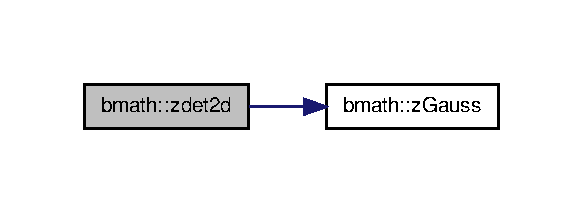
\includegraphics[width=280pt]{namespacebmath_a94ae3022a9719013e6bf0d5e5230c81c_cgraph}
\end{center}
\end{figure}


\hypertarget{namespacebmath_ac569fe0169cdaadfacf9236f3d1b4410}{
\index{bmath@{bmath}!zGauss@{zGauss}}
\index{zGauss@{zGauss}!bmath@{bmath}}
\subsubsection[{zGauss}]{\setlength{\rightskip}{0pt plus 5cm}subroutine bmath::zGauss (
\begin{DoxyParamCaption}
\item[{integer,intent(in)}]{n, }
\item[{complex$\ast$16,dimension(n,n),intent(inout)}]{a, }
\item[{integer,dimension(n),intent(out)}]{l}
\end{DoxyParamCaption}
)}}
\label{namespacebmath_ac569fe0169cdaadfacf9236f3d1b4410}


Definition at line 138 of file bmath.f90.



Here is the caller graph for this function:
\nopagebreak
\begin{figure}[H]
\begin{center}
\leavevmode
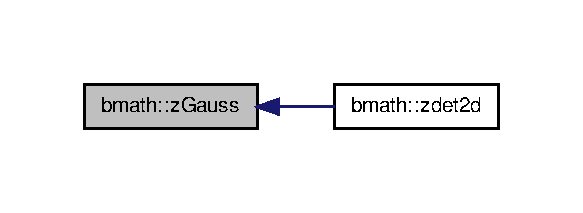
\includegraphics[width=280pt]{namespacebmath_ac569fe0169cdaadfacf9236f3d1b4410_icgraph}
\end{center}
\end{figure}


\hypertarget{namespacebmath_a75f76714b32b64ea7e2f8d78fac52f52}{
\index{bmath@{bmath}!zlin\_\-int@{zlin\_\-int}}
\index{zlin\_\-int@{zlin\_\-int}!bmath@{bmath}}
\subsubsection[{zlin\_\-int}]{\setlength{\rightskip}{0pt plus 5cm}subroutine bmath::zlin\_\-int (
\begin{DoxyParamCaption}
\item[{real$\ast$8,dimension(n),intent(in)}]{xa, }
\item[{complex$\ast$16,dimension(n),intent(in)}]{ya, }
\item[{integer,intent(in)}]{n, }
\item[{real$\ast$8,intent(in)}]{x, }
\item[{complex$\ast$16,intent(out)}]{y, }
\item[{integer,intent(inout)}]{ki}
\end{DoxyParamCaption}
)}}
\label{namespacebmath_a75f76714b32b64ea7e2f8d78fac52f52}


Definition at line 199 of file bmath.f90.


\hypertarget{namespacebstring}{
\section{bstring Module Reference}
\label{namespacebstring}\index{bstring@{bstring}}
}
\subsection*{Functions/Subroutines}
\begin{DoxyCompactItemize}
\item 
subroutine \hyperlink{namespacebstring_ae0c89d93b4c1e880651406a18b1feca5}{findFirstWord} (line, delimiters, istart, iend)
\item 
character \hyperlink{namespacebstring_a7a483e4b0c8d5c0a589a2c0980e6b961}{getFirstNonBlankChar} (chararr)
\item 
logical \hyperlink{namespacebstring_a0c60c1f333eef065d2b996aa4df5227e}{isComment} (line)
\end{DoxyCompactItemize}


\subsection{Function/Subroutine Documentation}
\hypertarget{namespacebstring_ae0c89d93b4c1e880651406a18b1feca5}{
\index{bstring@{bstring}!findFirstWord@{findFirstWord}}
\index{findFirstWord@{findFirstWord}!bstring@{bstring}}
\subsubsection[{findFirstWord}]{\setlength{\rightskip}{0pt plus 5cm}subroutine bstring::findFirstWord (
\begin{DoxyParamCaption}
\item[{character(len=$\ast$),intent(in)}]{line, }
\item[{character(len=$\ast$),intent(in)}]{delimiters, }
\item[{integer,intent(out)}]{istart, }
\item[{integer,intent(out)}]{iend}
\end{DoxyParamCaption}
)}}
\label{namespacebstring_ae0c89d93b4c1e880651406a18b1feca5}


Definition at line 28 of file bstring.f90.



Here is the caller graph for this function:\nopagebreak
\begin{figure}[H]
\begin{center}
\leavevmode
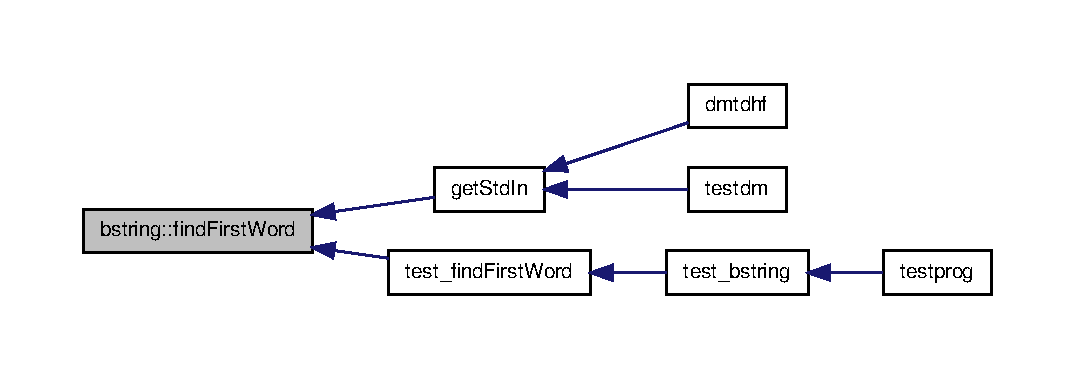
\includegraphics[width=400pt]{namespacebstring_ae0c89d93b4c1e880651406a18b1feca5_icgraph}
\end{center}
\end{figure}


\hypertarget{namespacebstring_a7a483e4b0c8d5c0a589a2c0980e6b961}{
\index{bstring@{bstring}!getFirstNonBlankChar@{getFirstNonBlankChar}}
\index{getFirstNonBlankChar@{getFirstNonBlankChar}!bstring@{bstring}}
\subsubsection[{getFirstNonBlankChar}]{\setlength{\rightskip}{0pt plus 5cm}character bstring::getFirstNonBlankChar (
\begin{DoxyParamCaption}
\item[{character(len=$\ast$),intent(in)}]{chararr}
\end{DoxyParamCaption}
)}}
\label{namespacebstring_a7a483e4b0c8d5c0a589a2c0980e6b961}


Definition at line 73 of file bstring.f90.



Here is the caller graph for this function:\nopagebreak
\begin{figure}[H]
\begin{center}
\leavevmode
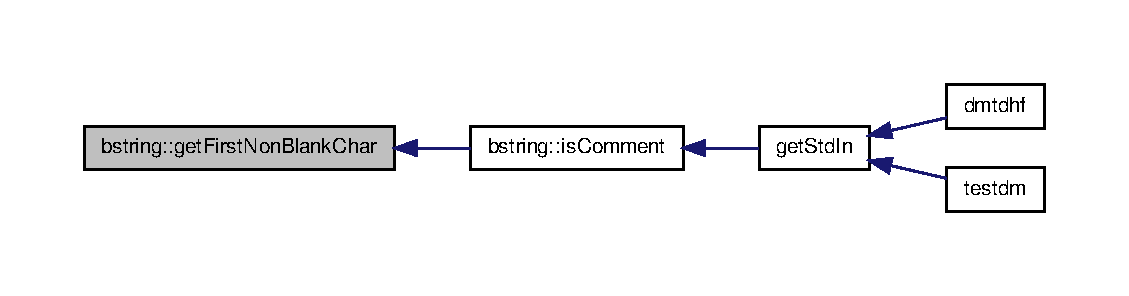
\includegraphics[width=400pt]{namespacebstring_a7a483e4b0c8d5c0a589a2c0980e6b961_icgraph}
\end{center}
\end{figure}


\hypertarget{namespacebstring_a0c60c1f333eef065d2b996aa4df5227e}{
\index{bstring@{bstring}!isComment@{isComment}}
\index{isComment@{isComment}!bstring@{bstring}}
\subsubsection[{isComment}]{\setlength{\rightskip}{0pt plus 5cm}logical bstring::isComment (
\begin{DoxyParamCaption}
\item[{character(len=$\ast$)}]{line}
\end{DoxyParamCaption}
)}}
\label{namespacebstring_a0c60c1f333eef065d2b996aa4df5227e}


Definition at line 89 of file bstring.f90.



Here is the call graph for this function:\nopagebreak
\begin{figure}[H]
\begin{center}
\leavevmode
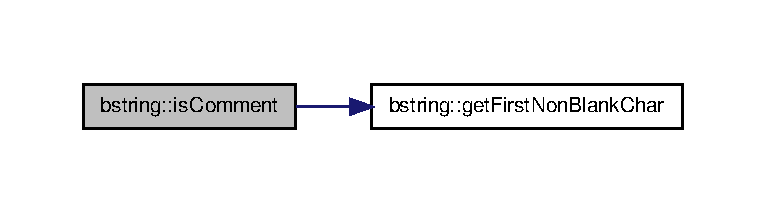
\includegraphics[width=368pt]{namespacebstring_a0c60c1f333eef065d2b996aa4df5227e_cgraph}
\end{center}
\end{figure}




Here is the caller graph for this function:\nopagebreak
\begin{figure}[H]
\begin{center}
\leavevmode
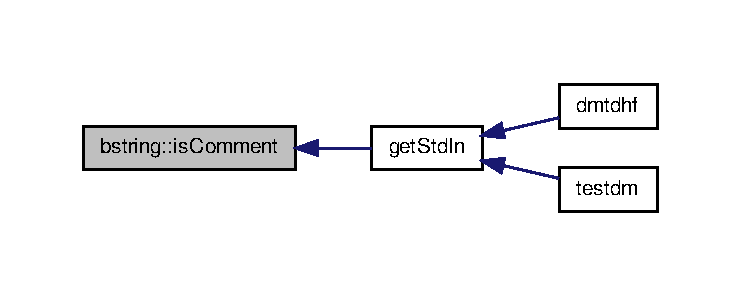
\includegraphics[width=356pt]{namespacebstring_a0c60c1f333eef065d2b996aa4df5227e_icgraph}
\end{center}
\end{figure}



\hypertarget{namespaceclass__ArrayList}{
\section{class\_\-ArrayList Module Reference}
\label{namespaceclass__ArrayList}\index{class\_\-ArrayList@{class\_\-ArrayList}}
}
\subsection*{Data Types}
\begin{DoxyCompactItemize}
\item 
type \hyperlink{typeclass__ArrayList_1_1dArrayList}{dArrayList}
\end{DoxyCompactItemize}
\subsection*{Functions/Subroutines}
\begin{DoxyCompactItemize}
\item 
type(\hyperlink{typeclass__ArrayList_1_1dArrayList}{dArrayList}) \hyperlink{namespaceclass__ArrayList_a5363f41df7698922433c25c73d02173d}{make\_\-dArrayList} (initLength)
\item 
subroutine \hyperlink{namespaceclass__ArrayList_a87eba505c7caff1cf303b9f92182aab2}{dArrayList\_\-add} (list, newValue)
\item 
subroutine \hyperlink{namespaceclass__ArrayList_a772b1369610a1b6481ef81093a7ecadf}{dArrayList\_\-ensureCapacity} (list, newCapacity)
\item 
real $\ast$8 \hyperlink{namespaceclass__ArrayList_a956a11e0e4778170667c2e90c9097766}{dArrayList\_\-get} (list, indix)
\item 
subroutine \hyperlink{namespaceclass__ArrayList_ad92f2ac90292027093572f20b4be9dc6}{dArrayList\_\-set} (list, indix, val)
\item 
integer \hyperlink{namespaceclass__ArrayList_a723eb1c041604ffeb1a0434c521de640}{dArrayList\_\-size} (list)
\end{DoxyCompactItemize}
\subsection*{Variables}
\begin{DoxyCompactItemize}
\item 
integer, parameter, private \hyperlink{namespaceclass__ArrayList_a710a353a125e9fcbc6bbb0fc3a468afb}{INITIAL\_\-LENGTH} = 10
\end{DoxyCompactItemize}


\subsection{Function/Subroutine Documentation}
\hypertarget{namespaceclass__ArrayList_a87eba505c7caff1cf303b9f92182aab2}{
\index{class\_\-ArrayList@{class\_\-ArrayList}!dArrayList\_\-add@{dArrayList\_\-add}}
\index{dArrayList\_\-add@{dArrayList\_\-add}!class_ArrayList@{class\_\-ArrayList}}
\subsubsection[{dArrayList\_\-add}]{\setlength{\rightskip}{0pt plus 5cm}subroutine class\_\-ArrayList::dArrayList\_\-add (
\begin{DoxyParamCaption}
\item[{type (dArrayList),intent(inout)}]{list, }
\item[{real$\ast$8,intent(in)}]{newValue}
\end{DoxyParamCaption}
)}}
\label{namespaceclass__ArrayList_a87eba505c7caff1cf303b9f92182aab2}


Definition at line 57 of file class\_\-ArrayList.f90.

\hypertarget{namespaceclass__ArrayList_a772b1369610a1b6481ef81093a7ecadf}{
\index{class\_\-ArrayList@{class\_\-ArrayList}!dArrayList\_\-ensureCapacity@{dArrayList\_\-ensureCapacity}}
\index{dArrayList\_\-ensureCapacity@{dArrayList\_\-ensureCapacity}!class_ArrayList@{class\_\-ArrayList}}
\subsubsection[{dArrayList\_\-ensureCapacity}]{\setlength{\rightskip}{0pt plus 5cm}subroutine class\_\-ArrayList::dArrayList\_\-ensureCapacity (
\begin{DoxyParamCaption}
\item[{type (dArrayList),intent(inout)}]{list, }
\item[{integer,intent(in)}]{newCapacity}
\end{DoxyParamCaption}
)}}
\label{namespaceclass__ArrayList_a772b1369610a1b6481ef81093a7ecadf}


Definition at line 74 of file class\_\-ArrayList.f90.

\hypertarget{namespaceclass__ArrayList_a956a11e0e4778170667c2e90c9097766}{
\index{class\_\-ArrayList@{class\_\-ArrayList}!dArrayList\_\-get@{dArrayList\_\-get}}
\index{dArrayList\_\-get@{dArrayList\_\-get}!class_ArrayList@{class\_\-ArrayList}}
\subsubsection[{dArrayList\_\-get}]{\setlength{\rightskip}{0pt plus 5cm}real$\ast$8 class\_\-ArrayList::dArrayList\_\-get (
\begin{DoxyParamCaption}
\item[{type(dArrayList),intent(in)}]{list, }
\item[{integer,intent(in)}]{indix}
\end{DoxyParamCaption}
)}}
\label{namespaceclass__ArrayList_a956a11e0e4778170667c2e90c9097766}


Definition at line 88 of file class\_\-ArrayList.f90.

\hypertarget{namespaceclass__ArrayList_ad92f2ac90292027093572f20b4be9dc6}{
\index{class\_\-ArrayList@{class\_\-ArrayList}!dArrayList\_\-set@{dArrayList\_\-set}}
\index{dArrayList\_\-set@{dArrayList\_\-set}!class_ArrayList@{class\_\-ArrayList}}
\subsubsection[{dArrayList\_\-set}]{\setlength{\rightskip}{0pt plus 5cm}subroutine class\_\-ArrayList::dArrayList\_\-set (
\begin{DoxyParamCaption}
\item[{type(dArrayList),intent(inout)}]{list, }
\item[{integer,intent(in)}]{indix, }
\item[{real$\ast$8,intent(in)}]{val}
\end{DoxyParamCaption}
)}}
\label{namespaceclass__ArrayList_ad92f2ac90292027093572f20b4be9dc6}


Definition at line 108 of file class\_\-ArrayList.f90.

\hypertarget{namespaceclass__ArrayList_a723eb1c041604ffeb1a0434c521de640}{
\index{class\_\-ArrayList@{class\_\-ArrayList}!dArrayList\_\-size@{dArrayList\_\-size}}
\index{dArrayList\_\-size@{dArrayList\_\-size}!class_ArrayList@{class\_\-ArrayList}}
\subsubsection[{dArrayList\_\-size}]{\setlength{\rightskip}{0pt plus 5cm}integer class\_\-ArrayList::dArrayList\_\-size (
\begin{DoxyParamCaption}
\item[{type(dArrayList),intent(in)}]{list}
\end{DoxyParamCaption}
)}}
\label{namespaceclass__ArrayList_a723eb1c041604ffeb1a0434c521de640}


Definition at line 127 of file class\_\-ArrayList.f90.

\hypertarget{namespaceclass__ArrayList_a5363f41df7698922433c25c73d02173d}{
\index{class\_\-ArrayList@{class\_\-ArrayList}!make\_\-dArrayList@{make\_\-dArrayList}}
\index{make\_\-dArrayList@{make\_\-dArrayList}!class_ArrayList@{class\_\-ArrayList}}
\subsubsection[{make\_\-dArrayList}]{\setlength{\rightskip}{0pt plus 5cm}type ({\bf dArrayList}) class\_\-ArrayList::make\_\-dArrayList (
\begin{DoxyParamCaption}
\item[{integer,intent(in),optional}]{initLength}
\end{DoxyParamCaption}
)}}
\label{namespaceclass__ArrayList_a5363f41df7698922433c25c73d02173d}


Definition at line 38 of file class\_\-ArrayList.f90.



\subsection{Variable Documentation}
\hypertarget{namespaceclass__ArrayList_a710a353a125e9fcbc6bbb0fc3a468afb}{
\index{class\_\-ArrayList@{class\_\-ArrayList}!INITIAL\_\-LENGTH@{INITIAL\_\-LENGTH}}
\index{INITIAL\_\-LENGTH@{INITIAL\_\-LENGTH}!class_ArrayList@{class\_\-ArrayList}}
\subsubsection[{INITIAL\_\-LENGTH}]{\setlength{\rightskip}{0pt plus 5cm}integer,parameter,private {\bf class\_\-ArrayList::INITIAL\_\-LENGTH} = 10}}
\label{namespaceclass__ArrayList_a710a353a125e9fcbc6bbb0fc3a468afb}


Definition at line 27 of file class\_\-ArrayList.f90.


\hypertarget{namespaceclass__PhysicalQuantity}{
\section{class\_\-PhysicalQuantity Module Reference}
\label{namespaceclass__PhysicalQuantity}\index{class\_\-PhysicalQuantity@{class\_\-PhysicalQuantity}}
}
\subsection*{Data Types}
\begin{DoxyCompactItemize}
\item 
type \hyperlink{typeclass__PhysicalQuantity_1_1PhysicalQuantity}{PhysicalQuantity}
\begin{DoxyCompactList}\small\item\em Stores a quantity with a value, uncertainty, and units. \item\end{DoxyCompactList}\end{DoxyCompactItemize}
\subsection*{Functions/Subroutines}
\begin{DoxyCompactItemize}
\item 
type(physicalQuantity) \hyperlink{namespaceclass__PhysicalQuantity_a31d0e7291e89fca5b49f9484556cf0cb}{new\_\-PhysicalQuantity} (newSymbol, newDimensions, newVal, newUnc)
\begin{DoxyCompactList}\small\item\em Constructs new \hyperlink{typeclass__PhysicalQuantity_1_1PhysicalQuantity}{PhysicalQuantity}. Assumes the value and uncertainty are given in the current unit system. \item\end{DoxyCompactList}\end{DoxyCompactItemize}
\subsection*{Variables}
\begin{DoxyCompactItemize}
\item 
integer, parameter, private \hyperlink{namespaceclass__PhysicalQuantity_a2870256032bca15f690a32ce1d1b6c52}{MAX\_\-SYMBOL\_\-SIZE} = 5
\item 
type(\hyperlink{typeclass__UnitSystem_1_1UnitSystem}{UnitSystem}) \hyperlink{namespaceclass__PhysicalQuantity_a61173098b2362361938556f5fb35431e}{theUnitSystem} = UNIT\_\-SYSTEM\_\-SI
\begin{DoxyCompactList}\small\item\em This is the unit system that all quantities are defined in. By default, we use SI units. \item\end{DoxyCompactList}\item 
type(\hyperlink{typeclass__PhysicalQuantity_1_1PhysicalQuantity}{PhysicalQuantity}), parameter \hyperlink{namespaceclass__PhysicalQuantity_a0633cd9b4645d04d7d47dbd151837757}{METER} = \hyperlink{typeclass__PhysicalQuantity_1_1PhysicalQuantity}{PhysicalQuantity}(\char`\"{}m\char`\"{}, (/1,0,0,0,0,0,0/), 1, 0)
\item 
type(\hyperlink{typeclass__PhysicalQuantity_1_1PhysicalQuantity}{PhysicalQuantity}), parameter \hyperlink{namespaceclass__PhysicalQuantity_a902db03da895ab4c528d71d99e8549b0}{KILOGRAM} = \hyperlink{typeclass__PhysicalQuantity_1_1PhysicalQuantity}{PhysicalQuantity}(\char`\"{}kg\char`\"{}, (/0,1,0,0,0,0,0/), 1, 0)
\item 
type(\hyperlink{typeclass__PhysicalQuantity_1_1PhysicalQuantity}{PhysicalQuantity}), parameter \hyperlink{namespaceclass__PhysicalQuantity_a7fdf486aace5a1e99af5a634719bb9ce}{SECOND} = \hyperlink{typeclass__PhysicalQuantity_1_1PhysicalQuantity}{PhysicalQuantity}(\char`\"{}s\char`\"{}, (/0,0,1,0,0,0,0/), 1, 0)
\item 
type(\hyperlink{typeclass__PhysicalQuantity_1_1PhysicalQuantity}{PhysicalQuantity}), parameter \hyperlink{namespaceclass__PhysicalQuantity_a9672ba1ed56d49205a831ba235421de8}{AMPERE} = \hyperlink{typeclass__PhysicalQuantity_1_1PhysicalQuantity}{PhysicalQuantity}(\char`\"{}A\char`\"{}, (/0,0,0,1,0,0,0/), 1, 0)
\item 
type(\hyperlink{typeclass__PhysicalQuantity_1_1PhysicalQuantity}{PhysicalQuantity}), parameter \hyperlink{namespaceclass__PhysicalQuantity_a2fd77862111da187e89aaf75383baa00}{KELVIN} = \hyperlink{typeclass__PhysicalQuantity_1_1PhysicalQuantity}{PhysicalQuantity}(\char`\"{}K\char`\"{}, (/0,0,0,0,1,0,0/), 1, 0)
\item 
type(\hyperlink{typeclass__PhysicalQuantity_1_1PhysicalQuantity}{PhysicalQuantity}), parameter \hyperlink{namespaceclass__PhysicalQuantity_a22a20ab491923015030051550a34c977}{MOLE} = \hyperlink{typeclass__PhysicalQuantity_1_1PhysicalQuantity}{PhysicalQuantity}(\char`\"{}mol\char`\"{}, (/0,0,0,0,0,1,0/), 1, 0)
\item 
type(\hyperlink{typeclass__PhysicalQuantity_1_1PhysicalQuantity}{PhysicalQuantity}), parameter \hyperlink{namespaceclass__PhysicalQuantity_ad332548c0150950850a5fece3ef0e8d2}{CANDELA} = \hyperlink{typeclass__PhysicalQuantity_1_1PhysicalQuantity}{PhysicalQuantity}(\char`\"{}cd\char`\"{}, (/0,0,0,0,0,0,1/), 1, 0)
\end{DoxyCompactItemize}


\subsection{Function/Subroutine Documentation}
\hypertarget{namespaceclass__PhysicalQuantity_a31d0e7291e89fca5b49f9484556cf0cb}{
\index{class\_\-PhysicalQuantity@{class\_\-PhysicalQuantity}!new\_\-PhysicalQuantity@{new\_\-PhysicalQuantity}}
\index{new\_\-PhysicalQuantity@{new\_\-PhysicalQuantity}!class_PhysicalQuantity@{class\_\-PhysicalQuantity}}
\subsubsection[{new\_\-PhysicalQuantity}]{\setlength{\rightskip}{0pt plus 5cm}type (physicalQuantity) class\_\-PhysicalQuantity::new\_\-PhysicalQuantity (
\begin{DoxyParamCaption}
\item[{character($\ast$),intent(in)}]{newSymbol, }
\item[{real (Long),dimension(:),intent(in)}]{newDimensions, }
\item[{real (Long),intent(in),optional}]{newVal, }
\item[{real (Long),intent(in),optional}]{newUnc}
\end{DoxyParamCaption}
)}}
\label{namespaceclass__PhysicalQuantity_a31d0e7291e89fca5b49f9484556cf0cb}


Constructs new \hyperlink{typeclass__PhysicalQuantity_1_1PhysicalQuantity}{PhysicalQuantity}. Assumes the value and uncertainty are given in the current unit system. 


\begin{DoxyParams}{Parameters}
{\em newSymbol} & symbol of quantity\\
\hline
{\em newDimensions} & new dimensions\\
\hline
{\em newVal} & value of quantity\\
\hline
{\em newUnc} & uncertainty of quantity \\
\hline
\end{DoxyParams}


Definition at line 59 of file class\_\-PhysicalQuantity.f90.



\subsection{Variable Documentation}
\hypertarget{namespaceclass__PhysicalQuantity_a9672ba1ed56d49205a831ba235421de8}{
\index{class\_\-PhysicalQuantity@{class\_\-PhysicalQuantity}!AMPERE@{AMPERE}}
\index{AMPERE@{AMPERE}!class_PhysicalQuantity@{class\_\-PhysicalQuantity}}
\subsubsection[{AMPERE}]{\setlength{\rightskip}{0pt plus 5cm}type ({\bf PhysicalQuantity}),parameter {\bf class\_\-PhysicalQuantity::AMPERE} = {\bf PhysicalQuantity}(\char`\"{}A\char`\"{}, (/0,0,0,1,0,0,0/), 1, 0)}}
\label{namespaceclass__PhysicalQuantity_a9672ba1ed56d49205a831ba235421de8}


Definition at line 45 of file class\_\-PhysicalQuantity.f90.

\hypertarget{namespaceclass__PhysicalQuantity_ad332548c0150950850a5fece3ef0e8d2}{
\index{class\_\-PhysicalQuantity@{class\_\-PhysicalQuantity}!CANDELA@{CANDELA}}
\index{CANDELA@{CANDELA}!class_PhysicalQuantity@{class\_\-PhysicalQuantity}}
\subsubsection[{CANDELA}]{\setlength{\rightskip}{0pt plus 5cm}type ({\bf PhysicalQuantity}),parameter {\bf class\_\-PhysicalQuantity::CANDELA} = {\bf PhysicalQuantity}(\char`\"{}cd\char`\"{}, (/0,0,0,0,0,0,1/), 1, 0)}}
\label{namespaceclass__PhysicalQuantity_ad332548c0150950850a5fece3ef0e8d2}


Definition at line 45 of file class\_\-PhysicalQuantity.f90.

\hypertarget{namespaceclass__PhysicalQuantity_a2fd77862111da187e89aaf75383baa00}{
\index{class\_\-PhysicalQuantity@{class\_\-PhysicalQuantity}!KELVIN@{KELVIN}}
\index{KELVIN@{KELVIN}!class_PhysicalQuantity@{class\_\-PhysicalQuantity}}
\subsubsection[{KELVIN}]{\setlength{\rightskip}{0pt plus 5cm}type ({\bf PhysicalQuantity}),parameter {\bf class\_\-PhysicalQuantity::KELVIN} = {\bf PhysicalQuantity}(\char`\"{}K\char`\"{}, (/0,0,0,0,1,0,0/), 1, 0)}}
\label{namespaceclass__PhysicalQuantity_a2fd77862111da187e89aaf75383baa00}


Definition at line 45 of file class\_\-PhysicalQuantity.f90.

\hypertarget{namespaceclass__PhysicalQuantity_a902db03da895ab4c528d71d99e8549b0}{
\index{class\_\-PhysicalQuantity@{class\_\-PhysicalQuantity}!KILOGRAM@{KILOGRAM}}
\index{KILOGRAM@{KILOGRAM}!class_PhysicalQuantity@{class\_\-PhysicalQuantity}}
\subsubsection[{KILOGRAM}]{\setlength{\rightskip}{0pt plus 5cm}type ({\bf PhysicalQuantity}),parameter {\bf class\_\-PhysicalQuantity::KILOGRAM} = {\bf PhysicalQuantity}(\char`\"{}kg\char`\"{}, (/0,1,0,0,0,0,0/), 1, 0)}}
\label{namespaceclass__PhysicalQuantity_a902db03da895ab4c528d71d99e8549b0}


Definition at line 45 of file class\_\-PhysicalQuantity.f90.

\hypertarget{namespaceclass__PhysicalQuantity_a2870256032bca15f690a32ce1d1b6c52}{
\index{class\_\-PhysicalQuantity@{class\_\-PhysicalQuantity}!MAX\_\-SYMBOL\_\-SIZE@{MAX\_\-SYMBOL\_\-SIZE}}
\index{MAX\_\-SYMBOL\_\-SIZE@{MAX\_\-SYMBOL\_\-SIZE}!class_PhysicalQuantity@{class\_\-PhysicalQuantity}}
\subsubsection[{MAX\_\-SYMBOL\_\-SIZE}]{\setlength{\rightskip}{0pt plus 5cm}integer,parameter,private {\bf class\_\-PhysicalQuantity::MAX\_\-SYMBOL\_\-SIZE} = 5}}
\label{namespaceclass__PhysicalQuantity_a2870256032bca15f690a32ce1d1b6c52}


Definition at line 8 of file class\_\-PhysicalQuantity.f90.

\hypertarget{namespaceclass__PhysicalQuantity_a0633cd9b4645d04d7d47dbd151837757}{
\index{class\_\-PhysicalQuantity@{class\_\-PhysicalQuantity}!METER@{METER}}
\index{METER@{METER}!class_PhysicalQuantity@{class\_\-PhysicalQuantity}}
\subsubsection[{METER}]{\setlength{\rightskip}{0pt plus 5cm}type ({\bf PhysicalQuantity}),parameter {\bf class\_\-PhysicalQuantity::METER} = {\bf PhysicalQuantity}(\char`\"{}m\char`\"{}, (/1,0,0,0,0,0,0/), 1, 0)}}
\label{namespaceclass__PhysicalQuantity_a0633cd9b4645d04d7d47dbd151837757}


Definition at line 45 of file class\_\-PhysicalQuantity.f90.

\hypertarget{namespaceclass__PhysicalQuantity_a22a20ab491923015030051550a34c977}{
\index{class\_\-PhysicalQuantity@{class\_\-PhysicalQuantity}!MOLE@{MOLE}}
\index{MOLE@{MOLE}!class_PhysicalQuantity@{class\_\-PhysicalQuantity}}
\subsubsection[{MOLE}]{\setlength{\rightskip}{0pt plus 5cm}type ({\bf PhysicalQuantity}),parameter {\bf class\_\-PhysicalQuantity::MOLE} = {\bf PhysicalQuantity}(\char`\"{}mol\char`\"{}, (/0,0,0,0,0,1,0/), 1, 0)}}
\label{namespaceclass__PhysicalQuantity_a22a20ab491923015030051550a34c977}


Definition at line 45 of file class\_\-PhysicalQuantity.f90.

\hypertarget{namespaceclass__PhysicalQuantity_a7fdf486aace5a1e99af5a634719bb9ce}{
\index{class\_\-PhysicalQuantity@{class\_\-PhysicalQuantity}!SECOND@{SECOND}}
\index{SECOND@{SECOND}!class_PhysicalQuantity@{class\_\-PhysicalQuantity}}
\subsubsection[{SECOND}]{\setlength{\rightskip}{0pt plus 5cm}type ({\bf PhysicalQuantity}),parameter {\bf class\_\-PhysicalQuantity::SECOND} = {\bf PhysicalQuantity}(\char`\"{}s\char`\"{}, (/0,0,1,0,0,0,0/), 1, 0)}}
\label{namespaceclass__PhysicalQuantity_a7fdf486aace5a1e99af5a634719bb9ce}


Definition at line 45 of file class\_\-PhysicalQuantity.f90.

\hypertarget{namespaceclass__PhysicalQuantity_a61173098b2362361938556f5fb35431e}{
\index{class\_\-PhysicalQuantity@{class\_\-PhysicalQuantity}!theUnitSystem@{theUnitSystem}}
\index{theUnitSystem@{theUnitSystem}!class_PhysicalQuantity@{class\_\-PhysicalQuantity}}
\subsubsection[{theUnitSystem}]{\setlength{\rightskip}{0pt plus 5cm}type({\bf UnitSystem}) {\bf class\_\-PhysicalQuantity::theUnitSystem} = UNIT\_\-SYSTEM\_\-SI}}
\label{namespaceclass__PhysicalQuantity_a61173098b2362361938556f5fb35431e}


This is the unit system that all quantities are defined in. By default, we use SI units. 



Definition at line 12 of file class\_\-PhysicalQuantity.f90.


\hypertarget{namespacecons__laws}{
\section{cons\_\-laws Module Reference}
\label{namespacecons__laws}\index{cons\_\-laws@{cons\_\-laws}}
}
\subsection*{Variables}
\begin{DoxyCompactItemize}
\item 
real(Long) \hyperlink{namespacecons__laws_a8d6ef7d1726b52d17e21c62607c22c3b}{ekin}
\item 
real(Long) \hyperlink{namespacecons__laws_aaaca27b785c52ee051b7f12c73182924}{ekerr}
\item 
real(Long) \hyperlink{namespacecons__laws_a1a3384f3d97911851a7c728ae1cd8af7}{ek0}
\item 
real(Long) \hyperlink{namespacecons__laws_a2d6e39be272e86946cd52d0596c6bc3a}{ek0err}
\item 
real(Long), dimension(:), allocatable \hyperlink{namespacecons__laws_a5e16e552d92dd5dd52c3cdc8600e62fe}{potx}
\item 
real(Long) \hyperlink{namespacecons__laws_a63e2f83fe00d6af9a68267f70281beac}{epot}
\item 
real(Long) \hyperlink{namespacecons__laws_a1fa58c36c9b57ed4261fddafdadfb924}{eperr}
\item 
real(Long) \hyperlink{namespacecons__laws_a1241ed7a0d2ec35982d18efa725fd588}{ep0}
\item 
real(Long) \hyperlink{namespacecons__laws_a9552ba8aaa6ba5048797e3dcabad3eb4}{ep0err}
\item 
real(Long) \hyperlink{namespacecons__laws_ac8202a23f94b9d534dfc7d5169d2e4bf}{nnum}
\end{DoxyCompactItemize}


\subsection{Variable Documentation}
\hypertarget{namespacecons__laws_a1a3384f3d97911851a7c728ae1cd8af7}{
\index{cons\_\-laws@{cons\_\-laws}!ek0@{ek0}}
\index{ek0@{ek0}!cons_laws@{cons\_\-laws}}
\subsubsection[{ek0}]{\setlength{\rightskip}{0pt plus 5cm}real (Long) {\bf cons\_\-laws::ek0}}}
\label{namespacecons__laws_a1a3384f3d97911851a7c728ae1cd8af7}


Definition at line 7 of file cons\_\-laws.f90.

\hypertarget{namespacecons__laws_a2d6e39be272e86946cd52d0596c6bc3a}{
\index{cons\_\-laws@{cons\_\-laws}!ek0err@{ek0err}}
\index{ek0err@{ek0err}!cons_laws@{cons\_\-laws}}
\subsubsection[{ek0err}]{\setlength{\rightskip}{0pt plus 5cm}real (Long) {\bf cons\_\-laws::ek0err}}}
\label{namespacecons__laws_a2d6e39be272e86946cd52d0596c6bc3a}


Definition at line 8 of file cons\_\-laws.f90.

\hypertarget{namespacecons__laws_aaaca27b785c52ee051b7f12c73182924}{
\index{cons\_\-laws@{cons\_\-laws}!ekerr@{ekerr}}
\index{ekerr@{ekerr}!cons_laws@{cons\_\-laws}}
\subsubsection[{ekerr}]{\setlength{\rightskip}{0pt plus 5cm}real (Long) {\bf cons\_\-laws::ekerr}}}
\label{namespacecons__laws_aaaca27b785c52ee051b7f12c73182924}


Definition at line 6 of file cons\_\-laws.f90.

\hypertarget{namespacecons__laws_a8d6ef7d1726b52d17e21c62607c22c3b}{
\index{cons\_\-laws@{cons\_\-laws}!ekin@{ekin}}
\index{ekin@{ekin}!cons_laws@{cons\_\-laws}}
\subsubsection[{ekin}]{\setlength{\rightskip}{0pt plus 5cm}real (Long) {\bf cons\_\-laws::ekin}}}
\label{namespacecons__laws_a8d6ef7d1726b52d17e21c62607c22c3b}


Definition at line 5 of file cons\_\-laws.f90.

\hypertarget{namespacecons__laws_a1241ed7a0d2ec35982d18efa725fd588}{
\index{cons\_\-laws@{cons\_\-laws}!ep0@{ep0}}
\index{ep0@{ep0}!cons_laws@{cons\_\-laws}}
\subsubsection[{ep0}]{\setlength{\rightskip}{0pt plus 5cm}real (Long) {\bf cons\_\-laws::ep0}}}
\label{namespacecons__laws_a1241ed7a0d2ec35982d18efa725fd588}


Definition at line 13 of file cons\_\-laws.f90.

\hypertarget{namespacecons__laws_a9552ba8aaa6ba5048797e3dcabad3eb4}{
\index{cons\_\-laws@{cons\_\-laws}!ep0err@{ep0err}}
\index{ep0err@{ep0err}!cons_laws@{cons\_\-laws}}
\subsubsection[{ep0err}]{\setlength{\rightskip}{0pt plus 5cm}real (Long) {\bf cons\_\-laws::ep0err}}}
\label{namespacecons__laws_a9552ba8aaa6ba5048797e3dcabad3eb4}


Definition at line 14 of file cons\_\-laws.f90.

\hypertarget{namespacecons__laws_a1fa58c36c9b57ed4261fddafdadfb924}{
\index{cons\_\-laws@{cons\_\-laws}!eperr@{eperr}}
\index{eperr@{eperr}!cons_laws@{cons\_\-laws}}
\subsubsection[{eperr}]{\setlength{\rightskip}{0pt plus 5cm}real (Long) {\bf cons\_\-laws::eperr}}}
\label{namespacecons__laws_a1fa58c36c9b57ed4261fddafdadfb924}


Definition at line 12 of file cons\_\-laws.f90.

\hypertarget{namespacecons__laws_a63e2f83fe00d6af9a68267f70281beac}{
\index{cons\_\-laws@{cons\_\-laws}!epot@{epot}}
\index{epot@{epot}!cons_laws@{cons\_\-laws}}
\subsubsection[{epot}]{\setlength{\rightskip}{0pt plus 5cm}real (Long) {\bf cons\_\-laws::epot}}}
\label{namespacecons__laws_a63e2f83fe00d6af9a68267f70281beac}


Definition at line 11 of file cons\_\-laws.f90.

\hypertarget{namespacecons__laws_ac8202a23f94b9d534dfc7d5169d2e4bf}{
\index{cons\_\-laws@{cons\_\-laws}!nnum@{nnum}}
\index{nnum@{nnum}!cons_laws@{cons\_\-laws}}
\subsubsection[{nnum}]{\setlength{\rightskip}{0pt plus 5cm}real (Long) {\bf cons\_\-laws::nnum}}}
\label{namespacecons__laws_ac8202a23f94b9d534dfc7d5169d2e4bf}


Definition at line 16 of file cons\_\-laws.f90.

\hypertarget{namespacecons__laws_a5e16e552d92dd5dd52c3cdc8600e62fe}{
\index{cons\_\-laws@{cons\_\-laws}!potx@{potx}}
\index{potx@{potx}!cons_laws@{cons\_\-laws}}
\subsubsection[{potx}]{\setlength{\rightskip}{0pt plus 5cm}real (Long),dimension(:),allocatable {\bf cons\_\-laws::potx}}}
\label{namespacecons__laws_a5e16e552d92dd5dd52c3cdc8600e62fe}


Definition at line 10 of file cons\_\-laws.f90.


\hypertarget{namespaceformat}{
\section{format Module Reference}
\label{namespaceformat}\index{format@{format}}
}
\subsection*{Variables}
\begin{DoxyCompactItemize}
\item 
integer \hyperlink{namespaceformat_a35a6cb9f260951fd6bd7ba9144cfaf5e}{dummy}
\end{DoxyCompactItemize}


\subsection{Variable Documentation}
\hypertarget{namespaceformat_a35a6cb9f260951fd6bd7ba9144cfaf5e}{
\index{format@{format}!dummy@{dummy}}
\index{dummy@{dummy}!format@{format}}
\subsubsection[{dummy}]{\setlength{\rightskip}{0pt plus 5cm}integer {\bf format::dummy}}}
\label{namespaceformat_a35a6cb9f260951fd6bd7ba9144cfaf5e}


Definition at line 26 of file format.f90.


\hypertarget{namespaceformatting}{
\section{formatting Module Reference}
\label{namespaceformatting}\index{formatting@{formatting}}
}
\subsection*{Variables}
\begin{DoxyCompactItemize}
\item 
character(len=20), parameter \hyperlink{namespaceformatting_a552aa51d2fb15a338e371114fd02c6e1}{fr5} = \char`\"{}(5E17.9)\char`\"{}
\end{DoxyCompactItemize}


\subsection{Variable Documentation}
\hypertarget{namespaceformatting_a552aa51d2fb15a338e371114fd02c6e1}{
\index{formatting@{formatting}!fr5@{fr5}}
\index{fr5@{fr5}!formatting@{formatting}}
\subsubsection[{fr5}]{\setlength{\rightskip}{0pt plus 5cm}character(len=20),parameter {\bf formatting::fr5} = \char`\"{}(5E17.9)\char`\"{}}}
\label{namespaceformatting_a552aa51d2fb15a338e371114fd02c6e1}


Definition at line 4 of file formatting.f90.


\hypertarget{namespaceinput__parameters}{
\section{input\_\-parameters Module Reference}
\label{namespaceinput__parameters}\index{input\_\-parameters@{input\_\-parameters}}
}
\subsection*{Variables}
\begin{DoxyCompactItemize}
\item 
integer \hyperlink{namespaceinput__parameters_a27dbda031851f558814121445cf46ed9}{potInitial}
\item 
integer \hyperlink{namespaceinput__parameters_a2ccc9d711d290b3e33fbc675ed390af2}{potFinal}
\item 
real(Long) \hyperlink{namespaceinput__parameters_ac937498371c0568d2d4ed1e1ef034e1d}{ea}
\item 
integer \hyperlink{namespaceinput__parameters_a0c5bab2cbe910c8543c442cb9be582d0}{ntime}
\item 
REAL(Long) \hyperlink{namespaceinput__parameters_a42efff37bd453975f48e8485e5757acd}{delt}
\item 
integer \hyperlink{namespaceinput__parameters_a3db2ebb8fcd24f403d0c3bd05a38e4c2}{Nevt}
\item 
logical \hyperlink{namespaceinput__parameters_aa73f50863135132e72d9a9c93d2cadef}{useImCutoff}
\item 
real(Long) \hyperlink{namespaceinput__parameters_a3987174aef89a10227220b4e5bdecde6}{cutoff\_\-w0}
\item 
real(Long) \hyperlink{namespaceinput__parameters_a87f2d307b48a20f985ea0692b9dfebf6}{cutoff\_\-x0}
\item 
real(Long) \hyperlink{namespaceinput__parameters_a8e63bceb853ebd1124eda12568a0e57f}{cutoff\_\-d0}
\item 
real(Long) \hyperlink{namespaceinput__parameters_a1d8bbaa8b473b798cb43170831cc57ac}{initialSeparation}
\item 
logical \hyperlink{namespaceinput__parameters_add8bfc502078fcdca67fff41e00114f7}{initState\_\-gaussianNuclear}
\item 
REAL(long) \hyperlink{namespaceinput__parameters_a745c6398e72faacdaacba0cf01027565}{w}
\item 
REAL(long) \hyperlink{namespaceinput__parameters_ae3a25357531dd0d2b8c5c4cc2de073d9}{whm}
\item 
INTEGER \hyperlink{namespaceinput__parameters_a29545f09a06c5a3def5df7fdb5f966ab}{Nmax}
\item 
logical \hyperlink{namespaceinput__parameters_a794b8486b7ecd6258448887bce533681}{initState\_\-cosine}
\item 
integer \hyperlink{namespaceinput__parameters_ad5ff3d9c110be99ed08bbe970f1630c8}{initState\_\-cosine\_\-number}
\item 
real(Long) \hyperlink{namespaceinput__parameters_a51d2cc916f531fadef1a6f0729644174}{initState\_\-cosine\_\-norm}
\item 
real(Long) \hyperlink{namespaceinput__parameters_ac3a5530df841dc82b4819f34f1e44980}{initState\_\-cosine\_\-shift}
\item 
logical \hyperlink{namespaceinput__parameters_a727a13be305b5dde7955fd2d02f955e4}{initState\_\-plane}
\item 
integer \hyperlink{namespaceinput__parameters_a876ac6edc93b733aeb66f54aca167741}{initState\_\-plane\_\-number}
\item 
real(Long) \hyperlink{namespaceinput__parameters_a22ba3f1343580a0db34433e32279e365}{initState\_\-plane\_\-norm}
\item 
real(Long) \hyperlink{namespaceinput__parameters_a97253a3c66d919b8a99dd33c633d3bd8}{initState\_\-plane\_\-shift}
\item 
logical \hyperlink{namespaceinput__parameters_aae45dd03716b9ad9a0600a9d9a798935}{initState\_\-kdelta}
\item 
real(Long) \hyperlink{namespaceinput__parameters_a1b2e5c088ab1d39d896586d7fb18b142}{initState\_\-kdelta\_\-norm}
\item 
real(Long) \hyperlink{namespaceinput__parameters_a65eb9165c6a1fd054daefc2a96e7ae2a}{initState\_\-kdelta\_\-x0}
\item 
integer \hyperlink{namespaceinput__parameters_a127f71f45eade1f05ced1535e88c771d}{splitOperatorMethod}
\item 
logical \hyperlink{namespaceinput__parameters_a9672a1c90e65a2ecee350dd2dae64e03}{useImEvol}
\item 
integer \hyperlink{namespaceinput__parameters_ac0212885e38ab22a77411b20bec16420}{Nimev}
\item 
logical \hyperlink{namespaceinput__parameters_a504b6e2c93e4a4af47125d83d6e5d75d}{useFlipClone}
\item 
logical \hyperlink{namespaceinput__parameters_ac1165234d614ad278effaf2a7910888b}{useAdiabatic}
\item 
integer \hyperlink{namespaceinput__parameters_a2b1e4d8baaa62168d989002cf747b30b}{iadib}
\item 
integer \hyperlink{namespaceinput__parameters_a6e8306262594749651ff9230cb525363}{Nad}
\item 
real(Long) \hyperlink{namespaceinput__parameters_ab3ac3c45168fc6aafd02e70822154417}{tad}
\item 
real(Long) \hyperlink{namespaceinput__parameters_a8d452c8a3d45ee77279fc26867c74ed6}{wtad}
\end{DoxyCompactItemize}


\subsection{Variable Documentation}
\hypertarget{namespaceinput__parameters_a8e63bceb853ebd1124eda12568a0e57f}{
\index{input\_\-parameters@{input\_\-parameters}!cutoff\_\-d0@{cutoff\_\-d0}}
\index{cutoff\_\-d0@{cutoff\_\-d0}!input_parameters@{input\_\-parameters}}
\subsubsection[{cutoff\_\-d0}]{\setlength{\rightskip}{0pt plus 5cm}real (Long) {\bf input\_\-parameters::cutoff\_\-d0}}}
\label{namespaceinput__parameters_a8e63bceb853ebd1124eda12568a0e57f}


Definition at line 19 of file input\_\-parameters.f90.

\hypertarget{namespaceinput__parameters_a3987174aef89a10227220b4e5bdecde6}{
\index{input\_\-parameters@{input\_\-parameters}!cutoff\_\-w0@{cutoff\_\-w0}}
\index{cutoff\_\-w0@{cutoff\_\-w0}!input_parameters@{input\_\-parameters}}
\subsubsection[{cutoff\_\-w0}]{\setlength{\rightskip}{0pt plus 5cm}real (Long) {\bf input\_\-parameters::cutoff\_\-w0}}}
\label{namespaceinput__parameters_a3987174aef89a10227220b4e5bdecde6}


Definition at line 17 of file input\_\-parameters.f90.

\hypertarget{namespaceinput__parameters_a87f2d307b48a20f985ea0692b9dfebf6}{
\index{input\_\-parameters@{input\_\-parameters}!cutoff\_\-x0@{cutoff\_\-x0}}
\index{cutoff\_\-x0@{cutoff\_\-x0}!input_parameters@{input\_\-parameters}}
\subsubsection[{cutoff\_\-x0}]{\setlength{\rightskip}{0pt plus 5cm}real (Long) {\bf input\_\-parameters::cutoff\_\-x0}}}
\label{namespaceinput__parameters_a87f2d307b48a20f985ea0692b9dfebf6}


Definition at line 18 of file input\_\-parameters.f90.

\hypertarget{namespaceinput__parameters_a42efff37bd453975f48e8485e5757acd}{
\index{input\_\-parameters@{input\_\-parameters}!delt@{delt}}
\index{delt@{delt}!input_parameters@{input\_\-parameters}}
\subsubsection[{delt}]{\setlength{\rightskip}{0pt plus 5cm}REAL (Long) {\bf input\_\-parameters::delt}}}
\label{namespaceinput__parameters_a42efff37bd453975f48e8485e5757acd}


Definition at line 12 of file input\_\-parameters.f90.

\hypertarget{namespaceinput__parameters_ac937498371c0568d2d4ed1e1ef034e1d}{
\index{input\_\-parameters@{input\_\-parameters}!ea@{ea}}
\index{ea@{ea}!input_parameters@{input\_\-parameters}}
\subsubsection[{ea}]{\setlength{\rightskip}{0pt plus 5cm}real (Long) {\bf input\_\-parameters::ea}}}
\label{namespaceinput__parameters_ac937498371c0568d2d4ed1e1ef034e1d}


Definition at line 8 of file input\_\-parameters.f90.

\hypertarget{namespaceinput__parameters_a2b1e4d8baaa62168d989002cf747b30b}{
\index{input\_\-parameters@{input\_\-parameters}!iadib@{iadib}}
\index{iadib@{iadib}!input_parameters@{input\_\-parameters}}
\subsubsection[{iadib}]{\setlength{\rightskip}{0pt plus 5cm}integer {\bf input\_\-parameters::iadib}}}
\label{namespaceinput__parameters_a2b1e4d8baaa62168d989002cf747b30b}


Definition at line 55 of file input\_\-parameters.f90.

\hypertarget{namespaceinput__parameters_a1d8bbaa8b473b798cb43170831cc57ac}{
\index{input\_\-parameters@{input\_\-parameters}!initialSeparation@{initialSeparation}}
\index{initialSeparation@{initialSeparation}!input_parameters@{input\_\-parameters}}
\subsubsection[{initialSeparation}]{\setlength{\rightskip}{0pt plus 5cm}real (Long) {\bf input\_\-parameters::initialSeparation}}}
\label{namespaceinput__parameters_a1d8bbaa8b473b798cb43170831cc57ac}


Definition at line 21 of file input\_\-parameters.f90.

\hypertarget{namespaceinput__parameters_a794b8486b7ecd6258448887bce533681}{
\index{input\_\-parameters@{input\_\-parameters}!initState\_\-cosine@{initState\_\-cosine}}
\index{initState\_\-cosine@{initState\_\-cosine}!input_parameters@{input\_\-parameters}}
\subsubsection[{initState\_\-cosine}]{\setlength{\rightskip}{0pt plus 5cm}logical {\bf input\_\-parameters::initState\_\-cosine}}}
\label{namespaceinput__parameters_a794b8486b7ecd6258448887bce533681}


Definition at line 28 of file input\_\-parameters.f90.

\hypertarget{namespaceinput__parameters_a51d2cc916f531fadef1a6f0729644174}{
\index{input\_\-parameters@{input\_\-parameters}!initState\_\-cosine\_\-norm@{initState\_\-cosine\_\-norm}}
\index{initState\_\-cosine\_\-norm@{initState\_\-cosine\_\-norm}!input_parameters@{input\_\-parameters}}
\subsubsection[{initState\_\-cosine\_\-norm}]{\setlength{\rightskip}{0pt plus 5cm}real (Long) {\bf input\_\-parameters::initState\_\-cosine\_\-norm}}}
\label{namespaceinput__parameters_a51d2cc916f531fadef1a6f0729644174}


Definition at line 30 of file input\_\-parameters.f90.

\hypertarget{namespaceinput__parameters_ad5ff3d9c110be99ed08bbe970f1630c8}{
\index{input\_\-parameters@{input\_\-parameters}!initState\_\-cosine\_\-number@{initState\_\-cosine\_\-number}}
\index{initState\_\-cosine\_\-number@{initState\_\-cosine\_\-number}!input_parameters@{input\_\-parameters}}
\subsubsection[{initState\_\-cosine\_\-number}]{\setlength{\rightskip}{0pt plus 5cm}integer {\bf input\_\-parameters::initState\_\-cosine\_\-number}}}
\label{namespaceinput__parameters_ad5ff3d9c110be99ed08bbe970f1630c8}


Definition at line 29 of file input\_\-parameters.f90.

\hypertarget{namespaceinput__parameters_ac3a5530df841dc82b4819f34f1e44980}{
\index{input\_\-parameters@{input\_\-parameters}!initState\_\-cosine\_\-shift@{initState\_\-cosine\_\-shift}}
\index{initState\_\-cosine\_\-shift@{initState\_\-cosine\_\-shift}!input_parameters@{input\_\-parameters}}
\subsubsection[{initState\_\-cosine\_\-shift}]{\setlength{\rightskip}{0pt plus 5cm}real (Long) {\bf input\_\-parameters::initState\_\-cosine\_\-shift}}}
\label{namespaceinput__parameters_ac3a5530df841dc82b4819f34f1e44980}


Definition at line 31 of file input\_\-parameters.f90.

\hypertarget{namespaceinput__parameters_add8bfc502078fcdca67fff41e00114f7}{
\index{input\_\-parameters@{input\_\-parameters}!initState\_\-gaussianNuclear@{initState\_\-gaussianNuclear}}
\index{initState\_\-gaussianNuclear@{initState\_\-gaussianNuclear}!input_parameters@{input\_\-parameters}}
\subsubsection[{initState\_\-gaussianNuclear}]{\setlength{\rightskip}{0pt plus 5cm}logical {\bf input\_\-parameters::initState\_\-gaussianNuclear}}}
\label{namespaceinput__parameters_add8bfc502078fcdca67fff41e00114f7}


Definition at line 23 of file input\_\-parameters.f90.

\hypertarget{namespaceinput__parameters_aae45dd03716b9ad9a0600a9d9a798935}{
\index{input\_\-parameters@{input\_\-parameters}!initState\_\-kdelta@{initState\_\-kdelta}}
\index{initState\_\-kdelta@{initState\_\-kdelta}!input_parameters@{input\_\-parameters}}
\subsubsection[{initState\_\-kdelta}]{\setlength{\rightskip}{0pt plus 5cm}logical {\bf input\_\-parameters::initState\_\-kdelta}}}
\label{namespaceinput__parameters_aae45dd03716b9ad9a0600a9d9a798935}


Definition at line 38 of file input\_\-parameters.f90.

\hypertarget{namespaceinput__parameters_a1b2e5c088ab1d39d896586d7fb18b142}{
\index{input\_\-parameters@{input\_\-parameters}!initState\_\-kdelta\_\-norm@{initState\_\-kdelta\_\-norm}}
\index{initState\_\-kdelta\_\-norm@{initState\_\-kdelta\_\-norm}!input_parameters@{input\_\-parameters}}
\subsubsection[{initState\_\-kdelta\_\-norm}]{\setlength{\rightskip}{0pt plus 5cm}real (Long) {\bf input\_\-parameters::initState\_\-kdelta\_\-norm}}}
\label{namespaceinput__parameters_a1b2e5c088ab1d39d896586d7fb18b142}


Definition at line 39 of file input\_\-parameters.f90.

\hypertarget{namespaceinput__parameters_a65eb9165c6a1fd054daefc2a96e7ae2a}{
\index{input\_\-parameters@{input\_\-parameters}!initState\_\-kdelta\_\-x0@{initState\_\-kdelta\_\-x0}}
\index{initState\_\-kdelta\_\-x0@{initState\_\-kdelta\_\-x0}!input_parameters@{input\_\-parameters}}
\subsubsection[{initState\_\-kdelta\_\-x0}]{\setlength{\rightskip}{0pt plus 5cm}real (Long) {\bf input\_\-parameters::initState\_\-kdelta\_\-x0}}}
\label{namespaceinput__parameters_a65eb9165c6a1fd054daefc2a96e7ae2a}


Definition at line 40 of file input\_\-parameters.f90.

\hypertarget{namespaceinput__parameters_a727a13be305b5dde7955fd2d02f955e4}{
\index{input\_\-parameters@{input\_\-parameters}!initState\_\-plane@{initState\_\-plane}}
\index{initState\_\-plane@{initState\_\-plane}!input_parameters@{input\_\-parameters}}
\subsubsection[{initState\_\-plane}]{\setlength{\rightskip}{0pt plus 5cm}logical {\bf input\_\-parameters::initState\_\-plane}}}
\label{namespaceinput__parameters_a727a13be305b5dde7955fd2d02f955e4}


Definition at line 33 of file input\_\-parameters.f90.

\hypertarget{namespaceinput__parameters_a22ba3f1343580a0db34433e32279e365}{
\index{input\_\-parameters@{input\_\-parameters}!initState\_\-plane\_\-norm@{initState\_\-plane\_\-norm}}
\index{initState\_\-plane\_\-norm@{initState\_\-plane\_\-norm}!input_parameters@{input\_\-parameters}}
\subsubsection[{initState\_\-plane\_\-norm}]{\setlength{\rightskip}{0pt plus 5cm}real (Long) {\bf input\_\-parameters::initState\_\-plane\_\-norm}}}
\label{namespaceinput__parameters_a22ba3f1343580a0db34433e32279e365}


Definition at line 35 of file input\_\-parameters.f90.

\hypertarget{namespaceinput__parameters_a876ac6edc93b733aeb66f54aca167741}{
\index{input\_\-parameters@{input\_\-parameters}!initState\_\-plane\_\-number@{initState\_\-plane\_\-number}}
\index{initState\_\-plane\_\-number@{initState\_\-plane\_\-number}!input_parameters@{input\_\-parameters}}
\subsubsection[{initState\_\-plane\_\-number}]{\setlength{\rightskip}{0pt plus 5cm}integer {\bf input\_\-parameters::initState\_\-plane\_\-number}}}
\label{namespaceinput__parameters_a876ac6edc93b733aeb66f54aca167741}


Definition at line 34 of file input\_\-parameters.f90.

\hypertarget{namespaceinput__parameters_a97253a3c66d919b8a99dd33c633d3bd8}{
\index{input\_\-parameters@{input\_\-parameters}!initState\_\-plane\_\-shift@{initState\_\-plane\_\-shift}}
\index{initState\_\-plane\_\-shift@{initState\_\-plane\_\-shift}!input_parameters@{input\_\-parameters}}
\subsubsection[{initState\_\-plane\_\-shift}]{\setlength{\rightskip}{0pt plus 5cm}real (Long) {\bf input\_\-parameters::initState\_\-plane\_\-shift}}}
\label{namespaceinput__parameters_a97253a3c66d919b8a99dd33c633d3bd8}


Definition at line 36 of file input\_\-parameters.f90.

\hypertarget{namespaceinput__parameters_a6e8306262594749651ff9230cb525363}{
\index{input\_\-parameters@{input\_\-parameters}!Nad@{Nad}}
\index{Nad@{Nad}!input_parameters@{input\_\-parameters}}
\subsubsection[{Nad}]{\setlength{\rightskip}{0pt plus 5cm}integer {\bf input\_\-parameters::Nad}}}
\label{namespaceinput__parameters_a6e8306262594749651ff9230cb525363}


Definition at line 56 of file input\_\-parameters.f90.

\hypertarget{namespaceinput__parameters_a3db2ebb8fcd24f403d0c3bd05a38e4c2}{
\index{input\_\-parameters@{input\_\-parameters}!Nevt@{Nevt}}
\index{Nevt@{Nevt}!input_parameters@{input\_\-parameters}}
\subsubsection[{Nevt}]{\setlength{\rightskip}{0pt plus 5cm}integer {\bf input\_\-parameters::Nevt}}}
\label{namespaceinput__parameters_a3db2ebb8fcd24f403d0c3bd05a38e4c2}


Definition at line 13 of file input\_\-parameters.f90.

\hypertarget{namespaceinput__parameters_ac0212885e38ab22a77411b20bec16420}{
\index{input\_\-parameters@{input\_\-parameters}!Nimev@{Nimev}}
\index{Nimev@{Nimev}!input_parameters@{input\_\-parameters}}
\subsubsection[{Nimev}]{\setlength{\rightskip}{0pt plus 5cm}integer {\bf input\_\-parameters::Nimev}}}
\label{namespaceinput__parameters_ac0212885e38ab22a77411b20bec16420}


Definition at line 50 of file input\_\-parameters.f90.

\hypertarget{namespaceinput__parameters_a29545f09a06c5a3def5df7fdb5f966ab}{
\index{input\_\-parameters@{input\_\-parameters}!Nmax@{Nmax}}
\index{Nmax@{Nmax}!input_parameters@{input\_\-parameters}}
\subsubsection[{Nmax}]{\setlength{\rightskip}{0pt plus 5cm}INTEGER {\bf input\_\-parameters::Nmax}}}
\label{namespaceinput__parameters_a29545f09a06c5a3def5df7fdb5f966ab}


Definition at line 26 of file input\_\-parameters.f90.

\hypertarget{namespaceinput__parameters_a0c5bab2cbe910c8543c442cb9be582d0}{
\index{input\_\-parameters@{input\_\-parameters}!ntime@{ntime}}
\index{ntime@{ntime}!input_parameters@{input\_\-parameters}}
\subsubsection[{ntime}]{\setlength{\rightskip}{0pt plus 5cm}integer {\bf input\_\-parameters::ntime}}}
\label{namespaceinput__parameters_a0c5bab2cbe910c8543c442cb9be582d0}


Definition at line 10 of file input\_\-parameters.f90.

\hypertarget{namespaceinput__parameters_a2ccc9d711d290b3e33fbc675ed390af2}{
\index{input\_\-parameters@{input\_\-parameters}!potFinal@{potFinal}}
\index{potFinal@{potFinal}!input_parameters@{input\_\-parameters}}
\subsubsection[{potFinal}]{\setlength{\rightskip}{0pt plus 5cm}integer {\bf input\_\-parameters::potFinal}}}
\label{namespaceinput__parameters_a2ccc9d711d290b3e33fbc675ed390af2}


Definition at line 6 of file input\_\-parameters.f90.

\hypertarget{namespaceinput__parameters_a27dbda031851f558814121445cf46ed9}{
\index{input\_\-parameters@{input\_\-parameters}!potInitial@{potInitial}}
\index{potInitial@{potInitial}!input_parameters@{input\_\-parameters}}
\subsubsection[{potInitial}]{\setlength{\rightskip}{0pt plus 5cm}integer {\bf input\_\-parameters::potInitial}}}
\label{namespaceinput__parameters_a27dbda031851f558814121445cf46ed9}


Definition at line 5 of file input\_\-parameters.f90.

\hypertarget{namespaceinput__parameters_a127f71f45eade1f05ced1535e88c771d}{
\index{input\_\-parameters@{input\_\-parameters}!splitOperatorMethod@{splitOperatorMethod}}
\index{splitOperatorMethod@{splitOperatorMethod}!input_parameters@{input\_\-parameters}}
\subsubsection[{splitOperatorMethod}]{\setlength{\rightskip}{0pt plus 5cm}integer {\bf input\_\-parameters::splitOperatorMethod}}}
\label{namespaceinput__parameters_a127f71f45eade1f05ced1535e88c771d}


Definition at line 47 of file input\_\-parameters.f90.

\hypertarget{namespaceinput__parameters_ab3ac3c45168fc6aafd02e70822154417}{
\index{input\_\-parameters@{input\_\-parameters}!tad@{tad}}
\index{tad@{tad}!input_parameters@{input\_\-parameters}}
\subsubsection[{tad}]{\setlength{\rightskip}{0pt plus 5cm}real (Long) {\bf input\_\-parameters::tad}}}
\label{namespaceinput__parameters_ab3ac3c45168fc6aafd02e70822154417}


Definition at line 57 of file input\_\-parameters.f90.

\hypertarget{namespaceinput__parameters_ac1165234d614ad278effaf2a7910888b}{
\index{input\_\-parameters@{input\_\-parameters}!useAdiabatic@{useAdiabatic}}
\index{useAdiabatic@{useAdiabatic}!input_parameters@{input\_\-parameters}}
\subsubsection[{useAdiabatic}]{\setlength{\rightskip}{0pt plus 5cm}logical {\bf input\_\-parameters::useAdiabatic}}}
\label{namespaceinput__parameters_ac1165234d614ad278effaf2a7910888b}


Definition at line 54 of file input\_\-parameters.f90.

\hypertarget{namespaceinput__parameters_a504b6e2c93e4a4af47125d83d6e5d75d}{
\index{input\_\-parameters@{input\_\-parameters}!useFlipClone@{useFlipClone}}
\index{useFlipClone@{useFlipClone}!input_parameters@{input\_\-parameters}}
\subsubsection[{useFlipClone}]{\setlength{\rightskip}{0pt plus 5cm}logical {\bf input\_\-parameters::useFlipClone}}}
\label{namespaceinput__parameters_a504b6e2c93e4a4af47125d83d6e5d75d}


Definition at line 52 of file input\_\-parameters.f90.

\hypertarget{namespaceinput__parameters_aa73f50863135132e72d9a9c93d2cadef}{
\index{input\_\-parameters@{input\_\-parameters}!useImCutoff@{useImCutoff}}
\index{useImCutoff@{useImCutoff}!input_parameters@{input\_\-parameters}}
\subsubsection[{useImCutoff}]{\setlength{\rightskip}{0pt plus 5cm}logical {\bf input\_\-parameters::useImCutoff}}}
\label{namespaceinput__parameters_aa73f50863135132e72d9a9c93d2cadef}


Definition at line 16 of file input\_\-parameters.f90.

\hypertarget{namespaceinput__parameters_a9672a1c90e65a2ecee350dd2dae64e03}{
\index{input\_\-parameters@{input\_\-parameters}!useImEvol@{useImEvol}}
\index{useImEvol@{useImEvol}!input_parameters@{input\_\-parameters}}
\subsubsection[{useImEvol}]{\setlength{\rightskip}{0pt plus 5cm}logical {\bf input\_\-parameters::useImEvol}}}
\label{namespaceinput__parameters_a9672a1c90e65a2ecee350dd2dae64e03}


Definition at line 49 of file input\_\-parameters.f90.

\hypertarget{namespaceinput__parameters_a745c6398e72faacdaacba0cf01027565}{
\index{input\_\-parameters@{input\_\-parameters}!w@{w}}
\index{w@{w}!input_parameters@{input\_\-parameters}}
\subsubsection[{w}]{\setlength{\rightskip}{0pt plus 5cm}REAL (long) {\bf input\_\-parameters::w}}}
\label{namespaceinput__parameters_a745c6398e72faacdaacba0cf01027565}


Definition at line 24 of file input\_\-parameters.f90.

\hypertarget{namespaceinput__parameters_ae3a25357531dd0d2b8c5c4cc2de073d9}{
\index{input\_\-parameters@{input\_\-parameters}!whm@{whm}}
\index{whm@{whm}!input_parameters@{input\_\-parameters}}
\subsubsection[{whm}]{\setlength{\rightskip}{0pt plus 5cm}REAL (long) {\bf input\_\-parameters::whm}}}
\label{namespaceinput__parameters_ae3a25357531dd0d2b8c5c4cc2de073d9}


Definition at line 25 of file input\_\-parameters.f90.

\hypertarget{namespaceinput__parameters_a8d452c8a3d45ee77279fc26867c74ed6}{
\index{input\_\-parameters@{input\_\-parameters}!wtad@{wtad}}
\index{wtad@{wtad}!input_parameters@{input\_\-parameters}}
\subsubsection[{wtad}]{\setlength{\rightskip}{0pt plus 5cm}real (Long) {\bf input\_\-parameters::wtad}}}
\label{namespaceinput__parameters_a8d452c8a3d45ee77279fc26867c74ed6}


Definition at line 57 of file input\_\-parameters.f90.


\hypertarget{namespacelib__fftpack}{
\section{lib\_\-fftpack Module Reference}
\label{namespacelib__fftpack}\index{lib\_\-fftpack@{lib\_\-fftpack}}
}
\subsection*{Functions/Subroutines}
\begin{DoxyCompactItemize}
\item 
subroutine \hyperlink{namespacelib__fftpack_af2aa9b83c8db599ebc1c6067577196c0}{FT} (L, M, xre, xim)
\item 
subroutine \hyperlink{namespacelib__fftpack_af56d1d1be2bb706b859f005211a0c456}{IFT} (L, M, xre, xim)
\item 
subroutine \hyperlink{namespacelib__fftpack_a5c1e7931d9bdbe2b1ea0a987081b0515}{FFT2C} (L, M, xre, xim, fb)
\item 
subroutine \hyperlink{namespacelib__fftpack_a7f10fb88597cc6a353d06d4695e8087a}{FFT1} (L, M, xre, xim, fb)
\item 
subroutine \hyperlink{namespacelib__fftpack_aa19152959277a8d6578da7c1a6fc0230}{fft\_\-initial} (N)
\end{DoxyCompactItemize}
\subsection*{Variables}
\begin{DoxyCompactItemize}
\item 
INTEGER, dimension(2) \hyperlink{namespacelib__fftpack_ad1ac8096e29c8f4d4eccbbcd5ff74bf1}{lensav}
\item 
INTEGER, dimension(2) \hyperlink{namespacelib__fftpack_af22a24940af26c19850b9add69cc2adf}{lenwrk}
\item 
REAL(Long), dimension(:,:), allocatable \hyperlink{namespacelib__fftpack_ac4c893477b0614d957edb4530d018191}{work}
\item 
REAL(Long), dimension(:,:), allocatable \hyperlink{namespacelib__fftpack_a45c5d0eb1be9cdebf49b3c56e861d0d6}{wsavec}
\item 
REAL(Long), dimension(:,:), allocatable \hyperlink{namespacelib__fftpack_a6ab9f0bc33149a5032987f2f843f883e}{wsaves}
\end{DoxyCompactItemize}


\subsection{Function/Subroutine Documentation}
\hypertarget{namespacelib__fftpack_a7f10fb88597cc6a353d06d4695e8087a}{
\index{lib\_\-fftpack@{lib\_\-fftpack}!FFT1@{FFT1}}
\index{FFT1@{FFT1}!lib_fftpack@{lib\_\-fftpack}}
\subsubsection[{FFT1}]{\setlength{\rightskip}{0pt plus 5cm}subroutine lib\_\-fftpack::FFT1 (
\begin{DoxyParamCaption}
\item[{integer}]{L, }
\item[{integer}]{M, }
\item[{real (Long),dimension(l,m)}]{xre, }
\item[{real (Long),dimension(l,m)}]{xim, }
\item[{integer}]{fb}
\end{DoxyParamCaption}
)}}
\label{namespacelib__fftpack_a7f10fb88597cc6a353d06d4695e8087a}


Definition at line 157 of file lib\_\-fftpack.f90.



Here is the call graph for this function:\nopagebreak
\begin{figure}[H]
\begin{center}
\leavevmode
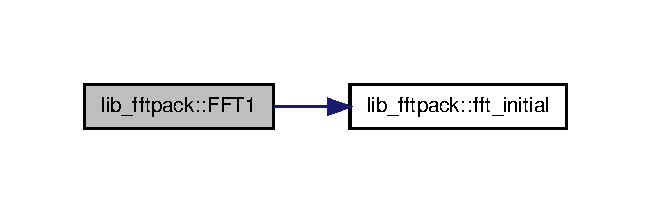
\includegraphics[width=312pt]{namespacelib__fftpack_a7f10fb88597cc6a353d06d4695e8087a_cgraph}
\end{center}
\end{figure}


\hypertarget{namespacelib__fftpack_a5c1e7931d9bdbe2b1ea0a987081b0515}{
\index{lib\_\-fftpack@{lib\_\-fftpack}!FFT2C@{FFT2C}}
\index{FFT2C@{FFT2C}!lib_fftpack@{lib\_\-fftpack}}
\subsubsection[{FFT2C}]{\setlength{\rightskip}{0pt plus 5cm}subroutine lib\_\-fftpack::FFT2C (
\begin{DoxyParamCaption}
\item[{integer}]{L, }
\item[{integer}]{M, }
\item[{real (Long),dimension(l,m)}]{xre, }
\item[{real (Long),dimension(l,m)}]{xim, }
\item[{integer}]{fb}
\end{DoxyParamCaption}
)}}
\label{namespacelib__fftpack_a5c1e7931d9bdbe2b1ea0a987081b0515}


Definition at line 105 of file lib\_\-fftpack.f90.



Here is the caller graph for this function:
\nopagebreak
\begin{figure}[H]
\begin{center}
\leavevmode
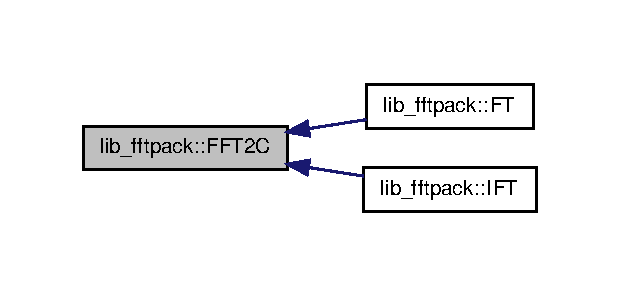
\includegraphics[width=298pt]{namespacelib__fftpack_a5c1e7931d9bdbe2b1ea0a987081b0515_icgraph}
\end{center}
\end{figure}


\hypertarget{namespacelib__fftpack_aa19152959277a8d6578da7c1a6fc0230}{
\index{lib\_\-fftpack@{lib\_\-fftpack}!fft\_\-initial@{fft\_\-initial}}
\index{fft\_\-initial@{fft\_\-initial}!lib_fftpack@{lib\_\-fftpack}}
\subsubsection[{fft\_\-initial}]{\setlength{\rightskip}{0pt plus 5cm}subroutine lib\_\-fftpack::fft\_\-initial (
\begin{DoxyParamCaption}
\item[{integer,dimension(2)}]{N}
\end{DoxyParamCaption}
)}}
\label{namespacelib__fftpack_aa19152959277a8d6578da7c1a6fc0230}


Definition at line 234 of file lib\_\-fftpack.f90.



Here is the caller graph for this function:
\nopagebreak
\begin{figure}[H]
\begin{center}
\leavevmode
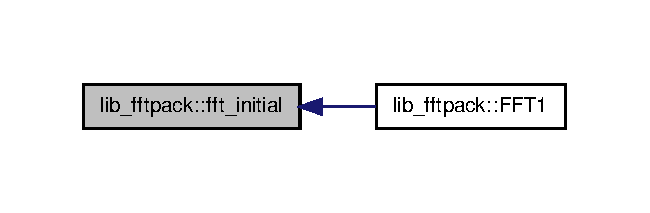
\includegraphics[width=312pt]{namespacelib__fftpack_aa19152959277a8d6578da7c1a6fc0230_icgraph}
\end{center}
\end{figure}


\hypertarget{namespacelib__fftpack_af2aa9b83c8db599ebc1c6067577196c0}{
\index{lib\_\-fftpack@{lib\_\-fftpack}!FT@{FT}}
\index{FT@{FT}!lib_fftpack@{lib\_\-fftpack}}
\subsubsection[{FT}]{\setlength{\rightskip}{0pt plus 5cm}subroutine lib\_\-fftpack::FT (
\begin{DoxyParamCaption}
\item[{integer}]{L, }
\item[{integer}]{M, }
\item[{real (Long),dimension(l,m)}]{xre, }
\item[{real (Long),dimension(l,m)}]{xim}
\end{DoxyParamCaption}
)}}
\label{namespacelib__fftpack_af2aa9b83c8db599ebc1c6067577196c0}


Definition at line 45 of file lib\_\-fftpack.f90.



Here is the call graph for this function:\nopagebreak
\begin{figure}[H]
\begin{center}
\leavevmode
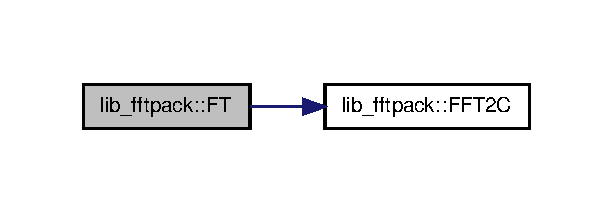
\includegraphics[width=294pt]{namespacelib__fftpack_af2aa9b83c8db599ebc1c6067577196c0_cgraph}
\end{center}
\end{figure}


\hypertarget{namespacelib__fftpack_af56d1d1be2bb706b859f005211a0c456}{
\index{lib\_\-fftpack@{lib\_\-fftpack}!IFT@{IFT}}
\index{IFT@{IFT}!lib_fftpack@{lib\_\-fftpack}}
\subsubsection[{IFT}]{\setlength{\rightskip}{0pt plus 5cm}subroutine lib\_\-fftpack::IFT (
\begin{DoxyParamCaption}
\item[{integer}]{L, }
\item[{integer}]{M, }
\item[{real (Long),dimension(l,m)}]{xre, }
\item[{real (Long),dimension(l,m)}]{xim}
\end{DoxyParamCaption}
)}}
\label{namespacelib__fftpack_af56d1d1be2bb706b859f005211a0c456}


Definition at line 75 of file lib\_\-fftpack.f90.



Here is the call graph for this function:\nopagebreak
\begin{figure}[H]
\begin{center}
\leavevmode
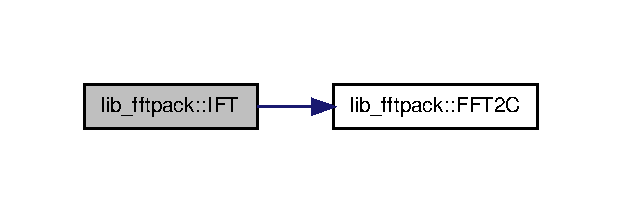
\includegraphics[width=298pt]{namespacelib__fftpack_af56d1d1be2bb706b859f005211a0c456_cgraph}
\end{center}
\end{figure}




\subsection{Variable Documentation}
\hypertarget{namespacelib__fftpack_ad1ac8096e29c8f4d4eccbbcd5ff74bf1}{
\index{lib\_\-fftpack@{lib\_\-fftpack}!lensav@{lensav}}
\index{lensav@{lensav}!lib_fftpack@{lib\_\-fftpack}}
\subsubsection[{lensav}]{\setlength{\rightskip}{0pt plus 5cm}INTEGER,dimension(2) {\bf lib\_\-fftpack::lensav}}}
\label{namespacelib__fftpack_ad1ac8096e29c8f4d4eccbbcd5ff74bf1}


Definition at line 28 of file lib\_\-fftpack.f90.

\hypertarget{namespacelib__fftpack_af22a24940af26c19850b9add69cc2adf}{
\index{lib\_\-fftpack@{lib\_\-fftpack}!lenwrk@{lenwrk}}
\index{lenwrk@{lenwrk}!lib_fftpack@{lib\_\-fftpack}}
\subsubsection[{lenwrk}]{\setlength{\rightskip}{0pt plus 5cm}INTEGER,dimension(2) {\bf lib\_\-fftpack::lenwrk}}}
\label{namespacelib__fftpack_af22a24940af26c19850b9add69cc2adf}


Definition at line 28 of file lib\_\-fftpack.f90.

\hypertarget{namespacelib__fftpack_ac4c893477b0614d957edb4530d018191}{
\index{lib\_\-fftpack@{lib\_\-fftpack}!work@{work}}
\index{work@{work}!lib_fftpack@{lib\_\-fftpack}}
\subsubsection[{work}]{\setlength{\rightskip}{0pt plus 5cm}REAL (Long),dimension(:,:),allocatable {\bf lib\_\-fftpack::work}}}
\label{namespacelib__fftpack_ac4c893477b0614d957edb4530d018191}


Definition at line 33 of file lib\_\-fftpack.f90.

\hypertarget{namespacelib__fftpack_a45c5d0eb1be9cdebf49b3c56e861d0d6}{
\index{lib\_\-fftpack@{lib\_\-fftpack}!wsavec@{wsavec}}
\index{wsavec@{wsavec}!lib_fftpack@{lib\_\-fftpack}}
\subsubsection[{wsavec}]{\setlength{\rightskip}{0pt plus 5cm}REAL (Long),dimension(:,:),allocatable {\bf lib\_\-fftpack::wsavec}}}
\label{namespacelib__fftpack_a45c5d0eb1be9cdebf49b3c56e861d0d6}


Definition at line 36 of file lib\_\-fftpack.f90.

\hypertarget{namespacelib__fftpack_a6ab9f0bc33149a5032987f2f843f883e}{
\index{lib\_\-fftpack@{lib\_\-fftpack}!wsaves@{wsaves}}
\index{wsaves@{wsaves}!lib_fftpack@{lib\_\-fftpack}}
\subsubsection[{wsaves}]{\setlength{\rightskip}{0pt plus 5cm}REAL (Long),dimension(:,:),allocatable {\bf lib\_\-fftpack::wsaves}}}
\label{namespacelib__fftpack_a6ab9f0bc33149a5032987f2f843f883e}


Definition at line 39 of file lib\_\-fftpack.f90.


\hypertarget{namespacelib__fftw}{
\section{lib\_\-fftw Module Reference}
\label{namespacelib__fftw}\index{lib\_\-fftw@{lib\_\-fftw}}
}
\subsection*{Functions/Subroutines}
\begin{DoxyCompactItemize}
\item 
subroutine \hyperlink{namespacelib__fftw_aa8927337a6ab7389c514e6460179570c}{ft\_\-z2z\_\-1d} (arrayin, arrayout, num)
\item 
subroutine \hyperlink{namespacelib__fftw_a29b8b749b6fc05610271170ebcce73b0}{ift\_\-z2z\_\-1d} (arrayin, arrayout, num)
\item 
subroutine \hyperlink{namespacelib__fftw_a2149f71532d3cff627c4683eb96553dc}{ft\_\-re\_\-1d} (arrayin, arrayout, num)
\item 
subroutine \hyperlink{namespacelib__fftw_a65faa306b75bb0444df109807bad2046}{ft\_\-ro\_\-1d} (arrayin, arrayout, num)
\end{DoxyCompactItemize}
\subsection*{Variables}
\begin{DoxyCompactItemize}
\item 
logical \hyperlink{namespacelib__fftw_a0c5a949d6fae23ba1b961780d217469e}{ft\_\-re\_\-1d\_\-init}
\end{DoxyCompactItemize}


\subsection{Function/Subroutine Documentation}
\hypertarget{namespacelib__fftw_a2149f71532d3cff627c4683eb96553dc}{
\index{lib\_\-fftw@{lib\_\-fftw}!ft\_\-re\_\-1d@{ft\_\-re\_\-1d}}
\index{ft\_\-re\_\-1d@{ft\_\-re\_\-1d}!lib_fftw@{lib\_\-fftw}}
\subsubsection[{ft\_\-re\_\-1d}]{\setlength{\rightskip}{0pt plus 5cm}subroutine lib\_\-fftw::ft\_\-re\_\-1d (
\begin{DoxyParamCaption}
\item[{real$\ast$8,dimension(0:num-\/1)}]{arrayin, }
\item[{real$\ast$8,dimension(0:num-\/1)}]{arrayout, }
\item[{integer,intent(in)}]{num}
\end{DoxyParamCaption}
)}}
\label{namespacelib__fftw_a2149f71532d3cff627c4683eb96553dc}


Definition at line 75 of file lib\_\-fftw.f90.



Here is the caller graph for this function:\nopagebreak
\begin{figure}[H]
\begin{center}
\leavevmode
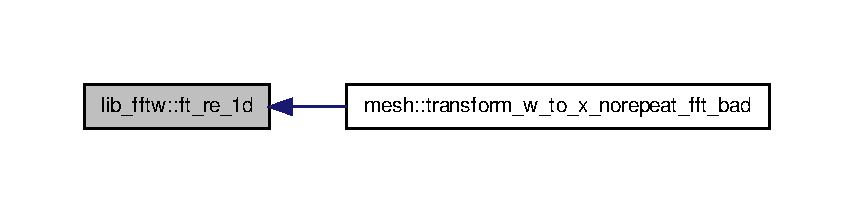
\includegraphics[width=400pt]{namespacelib__fftw_a2149f71532d3cff627c4683eb96553dc_icgraph}
\end{center}
\end{figure}


\hypertarget{namespacelib__fftw_a65faa306b75bb0444df109807bad2046}{
\index{lib\_\-fftw@{lib\_\-fftw}!ft\_\-ro\_\-1d@{ft\_\-ro\_\-1d}}
\index{ft\_\-ro\_\-1d@{ft\_\-ro\_\-1d}!lib_fftw@{lib\_\-fftw}}
\subsubsection[{ft\_\-ro\_\-1d}]{\setlength{\rightskip}{0pt plus 5cm}subroutine lib\_\-fftw::ft\_\-ro\_\-1d (
\begin{DoxyParamCaption}
\item[{real$\ast$8,dimension(0:num-\/1)}]{arrayin, }
\item[{real$\ast$8,dimension(0:num-\/1)}]{arrayout, }
\item[{integer,intent(in)}]{num}
\end{DoxyParamCaption}
)}}
\label{namespacelib__fftw_a65faa306b75bb0444df109807bad2046}


Definition at line 92 of file lib\_\-fftw.f90.



Here is the caller graph for this function:\nopagebreak
\begin{figure}[H]
\begin{center}
\leavevmode
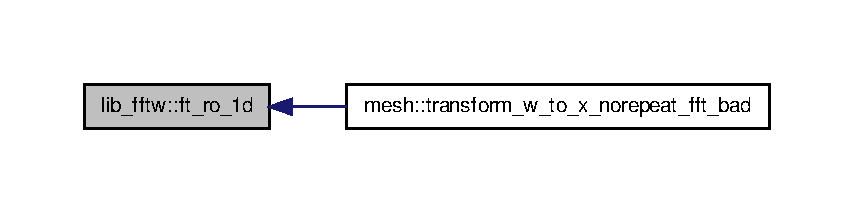
\includegraphics[width=400pt]{namespacelib__fftw_a65faa306b75bb0444df109807bad2046_icgraph}
\end{center}
\end{figure}


\hypertarget{namespacelib__fftw_aa8927337a6ab7389c514e6460179570c}{
\index{lib\_\-fftw@{lib\_\-fftw}!ft\_\-z2z\_\-1d@{ft\_\-z2z\_\-1d}}
\index{ft\_\-z2z\_\-1d@{ft\_\-z2z\_\-1d}!lib_fftw@{lib\_\-fftw}}
\subsubsection[{ft\_\-z2z\_\-1d}]{\setlength{\rightskip}{0pt plus 5cm}subroutine lib\_\-fftw::ft\_\-z2z\_\-1d (
\begin{DoxyParamCaption}
\item[{complex$\ast$16,dimension(0:num-\/1)}]{arrayin, }
\item[{complex$\ast$16,dimension(0:num-\/1)}]{arrayout, }
\item[{integer,intent(in)}]{num}
\end{DoxyParamCaption}
)}}
\label{namespacelib__fftw_aa8927337a6ab7389c514e6460179570c}


Definition at line 32 of file lib\_\-fftw.f90.



Here is the caller graph for this function:\nopagebreak
\begin{figure}[H]
\begin{center}
\leavevmode
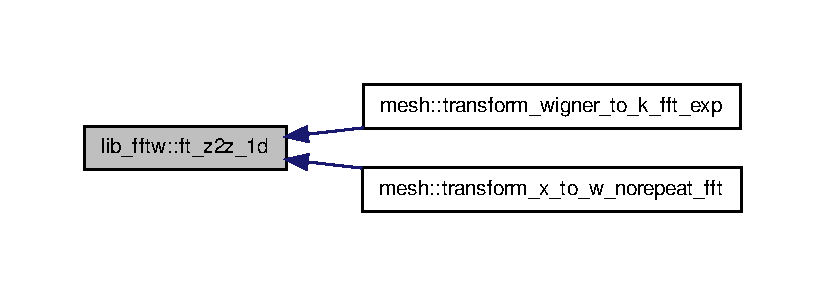
\includegraphics[width=400pt]{namespacelib__fftw_aa8927337a6ab7389c514e6460179570c_icgraph}
\end{center}
\end{figure}


\hypertarget{namespacelib__fftw_a29b8b749b6fc05610271170ebcce73b0}{
\index{lib\_\-fftw@{lib\_\-fftw}!ift\_\-z2z\_\-1d@{ift\_\-z2z\_\-1d}}
\index{ift\_\-z2z\_\-1d@{ift\_\-z2z\_\-1d}!lib_fftw@{lib\_\-fftw}}
\subsubsection[{ift\_\-z2z\_\-1d}]{\setlength{\rightskip}{0pt plus 5cm}subroutine lib\_\-fftw::ift\_\-z2z\_\-1d (
\begin{DoxyParamCaption}
\item[{complex$\ast$16,dimension(0:num-\/1)}]{arrayin, }
\item[{complex$\ast$16,dimension(0:num-\/1)}]{arrayout, }
\item[{integer,intent(in)}]{num}
\end{DoxyParamCaption}
)}}
\label{namespacelib__fftw_a29b8b749b6fc05610271170ebcce73b0}


Definition at line 56 of file lib\_\-fftw.f90.



Here is the caller graph for this function:\nopagebreak
\begin{figure}[H]
\begin{center}
\leavevmode
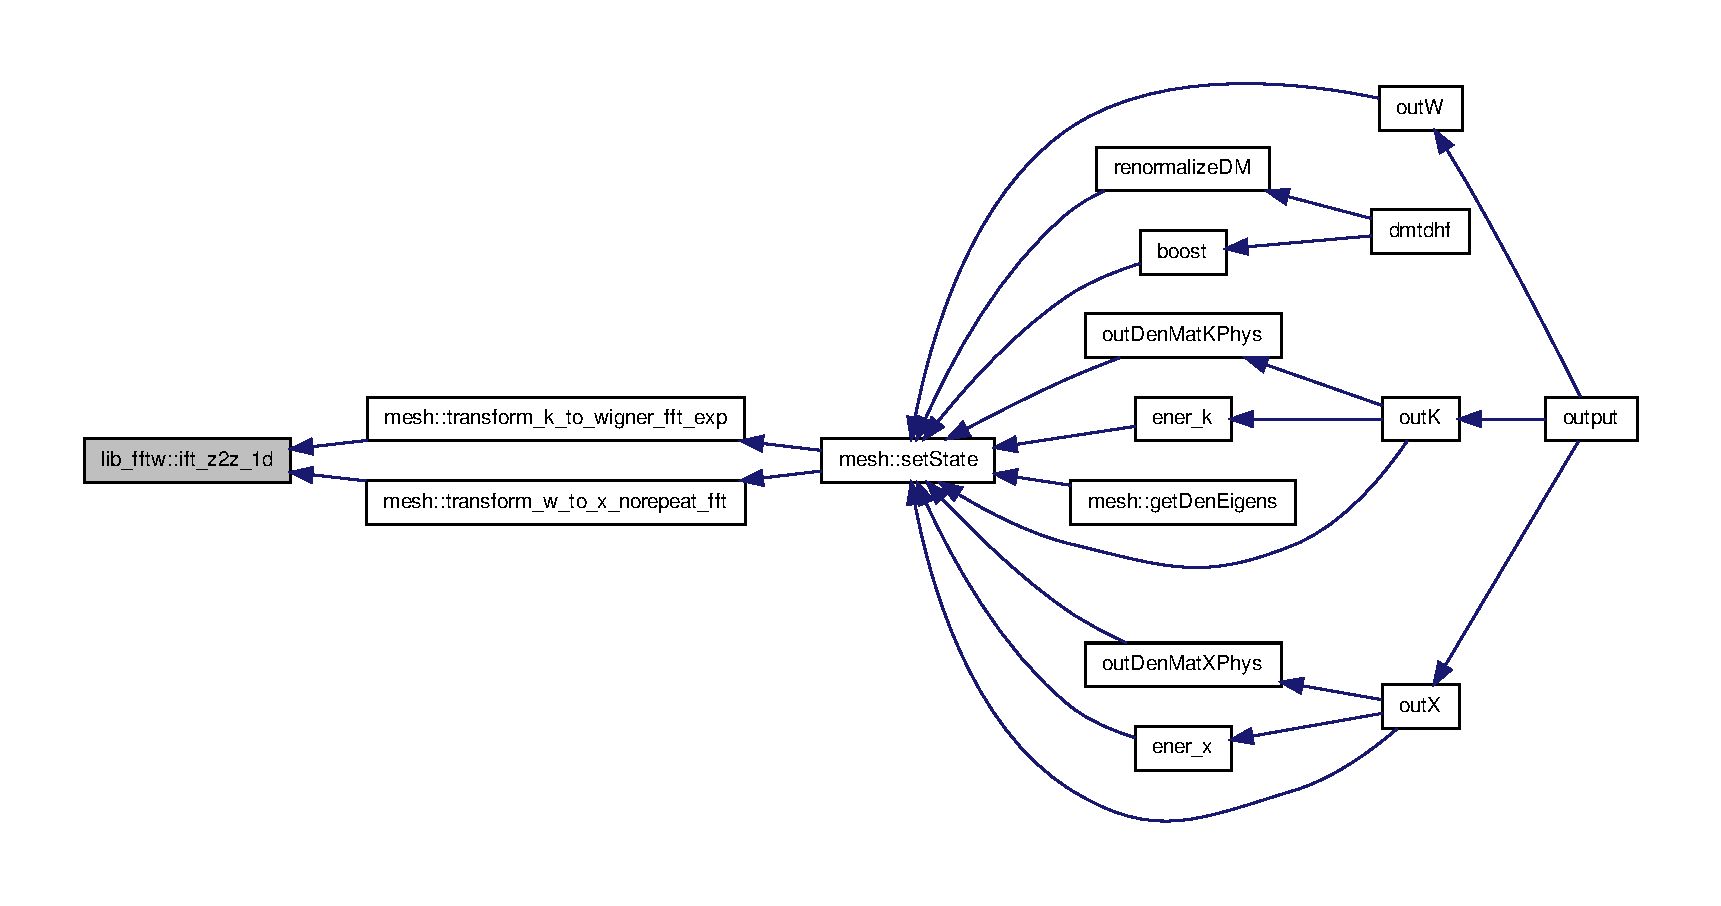
\includegraphics[width=400pt]{namespacelib__fftw_a29b8b749b6fc05610271170ebcce73b0_icgraph}
\end{center}
\end{figure}




\subsection{Variable Documentation}
\hypertarget{namespacelib__fftw_a0c5a949d6fae23ba1b961780d217469e}{
\index{lib\_\-fftw@{lib\_\-fftw}!ft\_\-re\_\-1d\_\-init@{ft\_\-re\_\-1d\_\-init}}
\index{ft\_\-re\_\-1d\_\-init@{ft\_\-re\_\-1d\_\-init}!lib_fftw@{lib\_\-fftw}}
\subsubsection[{ft\_\-re\_\-1d\_\-init}]{\setlength{\rightskip}{0pt plus 5cm}logical {\bf lib\_\-fftw::ft\_\-re\_\-1d\_\-init}}}
\label{namespacelib__fftw_a0c5a949d6fae23ba1b961780d217469e}


Definition at line 28 of file lib\_\-fftw.f90.


\hypertarget{namespacelib__lapack}{
\section{lib\_\-lapack Module Reference}
\label{namespacelib__lapack}\index{lib\_\-lapack@{lib\_\-lapack}}
}
\subsection*{Functions/Subroutines}
\begin{DoxyCompactItemize}
\item 
subroutine \hyperlink{namespacelib__lapack_a68a92047afc9e2ab7248d36406c53a0b}{getEigenSq} (mat, num, evals, evecs)
\item 
subroutine \hyperlink{namespacelib__lapack_a807f49d6f736971f5ee0eadce0af94eb}{getInvMat} (mat, num, matinv)
\end{DoxyCompactItemize}


\subsection{Function/Subroutine Documentation}
\hypertarget{namespacelib__lapack_a68a92047afc9e2ab7248d36406c53a0b}{
\index{lib\_\-lapack@{lib\_\-lapack}!getEigenSq@{getEigenSq}}
\index{getEigenSq@{getEigenSq}!lib_lapack@{lib\_\-lapack}}
\subsubsection[{getEigenSq}]{\setlength{\rightskip}{0pt plus 5cm}subroutine lib\_\-lapack::getEigenSq (
\begin{DoxyParamCaption}
\item[{complex$\ast$16,dimension(0:num-\/1,0:num-\/1),intent(inout)}]{mat, }
\item[{integer,intent(in)}]{num, }
\item[{complex$\ast$16,dimension(0:num-\/1),intent(out)}]{evals, }
\item[{complex$\ast$16,dimension(0:num-\/1,0:num-\/1),intent(inout)}]{evecs}
\end{DoxyParamCaption}
)}}
\label{namespacelib__lapack_a68a92047afc9e2ab7248d36406c53a0b}


Definition at line 27 of file lib\_\-lapack.f90.



Here is the caller graph for this function:
\nopagebreak
\begin{figure}[H]
\begin{center}
\leavevmode
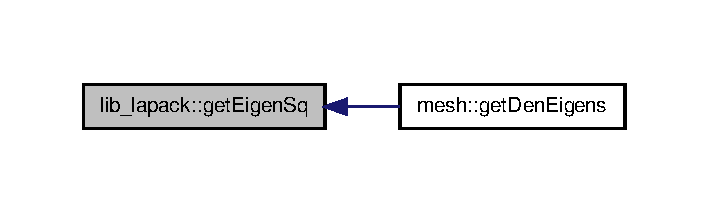
\includegraphics[width=340pt]{namespacelib__lapack_a68a92047afc9e2ab7248d36406c53a0b_icgraph}
\end{center}
\end{figure}


\hypertarget{namespacelib__lapack_a807f49d6f736971f5ee0eadce0af94eb}{
\index{lib\_\-lapack@{lib\_\-lapack}!getInvMat@{getInvMat}}
\index{getInvMat@{getInvMat}!lib_lapack@{lib\_\-lapack}}
\subsubsection[{getInvMat}]{\setlength{\rightskip}{0pt plus 5cm}subroutine lib\_\-lapack::getInvMat (
\begin{DoxyParamCaption}
\item[{complex$\ast$16,dimension(0:num-\/1,0:num-\/1),intent(in)}]{mat, }
\item[{integer,intent(in)}]{num, }
\item[{complex$\ast$16,dimension(0:num-\/1,0:num-\/1),intent(out)}]{matinv}
\end{DoxyParamCaption}
)}}
\label{namespacelib__lapack_a807f49d6f736971f5ee0eadce0af94eb}


Definition at line 74 of file lib\_\-lapack.f90.


\hypertarget{namespacemesh}{
\section{mesh Module Reference}
\label{namespacemesh}\index{mesh@{mesh}}
}
\subsection*{Functions/Subroutines}
\begin{DoxyCompactItemize}
\item 
integer \hyperlink{namespacemesh_ad1beeceb5580c23eb4fd6530573c395c}{getNearestIndexX} (xx)
\item 
subroutine \hyperlink{namespacemesh_a742012f09e48891eb9dd2a85601674a8}{initializeMesh}
\item 
complex $\ast$16 \hyperlink{namespacemesh_a30c07812e0215d470457c9be91bb6b65}{getDen} (i1, i2)
\item 
complex $\ast$16 \hyperlink{namespacemesh_af6c300cbff24f4eb25b428d822208430}{getDenDiagK} (ika)
\item 
complex $\ast$16 \hyperlink{namespacemesh_a87ae177a6a4383943393f8efa7da0018}{getDenX} (ixa, ixr)
\item 
subroutine \hyperlink{namespacemesh_abf02ca88d15c266099562e937ee507e4}{mesh\_\-reflectLR} ()
\item 
subroutine \hyperlink{namespacemesh_ac5a0f33502939ba9fae215e203d895f0}{mesh\_\-setReflectedLR} (reflect)
\item 
subroutine \hyperlink{namespacemesh_a7f55b8b4c3e045f04553b292c323b43a}{setDenX} (ixa, ixr, value)
\item 
complex $\ast$16 \hyperlink{namespacemesh_a54f9135de9933edd2a34168c4e5ebfca}{getDenW} (ixa, ika)
\item 
subroutine \hyperlink{namespacemesh_a7e79531a47425f91c6ac0921fc2203ed}{setDenW} (ixa, ika, this\_\-value)
\item 
complex $\ast$16 \hyperlink{namespacemesh_ab4cd19eafd4df4568c11c147b12f952d}{getDenK} (ikr, ika)
\item 
subroutine \hyperlink{namespacemesh_a16330a30f3f56c2944ef63240c049ee7}{setDenK} (ikr, ika, val)
\item 
subroutine \hyperlink{namespacemesh_ab3a026a1c77fc428f9a77f0ee37b0616}{getDenEigens} (evals, evecs)
\item 
subroutine \hyperlink{namespacemesh_aef51df23ee69f610420b25672a2da3ef}{setState} (state)
\item 
subroutine \hyperlink{namespacemesh_a0469cb1ff672271ea58fa1cca5daec7a}{transform\_\-x\_\-to\_\-wigner\_\-trig}
\item 
subroutine \hyperlink{namespacemesh_ab0c4d2eefb660f80c8bd5a26cfea90bb}{transform\_\-x\_\-to\_\-wigner\_\-dumb}
\item 
subroutine \hyperlink{namespacemesh_aedb02cc0a4ac5c08aef3398b9bca30be}{transform\_\-x\_\-to\_\-w\_\-dumb\_\-kshift}
\item 
subroutine \hyperlink{namespacemesh_af0c42421bd8b5b74a00094f639c4f7c7}{transform\_\-w\_\-to\_\-x\_\-norepeat\_\-fft}
\item 
subroutine \hyperlink{namespacemesh_ac641e03ceee3eaba6206a6e3b03db6af}{transform\_\-w\_\-to\_\-x\_\-norepeat\_\-fft\_\-bad}
\item 
subroutine \hyperlink{namespacemesh_a59d4c181b47238269732a26ba618696e}{transform\_\-wigner\_\-to\_\-x\_\-trig}
\item 
subroutine \hyperlink{namespacemesh_aee41613b43ab6e2f5a715e21c4227f4c}{transform\_\-wigner\_\-to\_\-x\_\-dumb}
\item 
subroutine \hyperlink{namespacemesh_ad6c116013ec5d5d4b1e8298749ffa481}{transform\_\-k\_\-to\_\-wigner\_\-trig}
\item 
subroutine \hyperlink{namespacemesh_affe8a5fb2705abf8f10cbac993ae66ff}{transform\_\-wigner\_\-to\_\-k\_\-trig}
\item 
subroutine \hyperlink{namespacemesh_ad10642a5ceb6239ab5dbf2124a221b45}{transform\_\-wigner\_\-to\_\-k\_\-dumb}
\item 
subroutine \hyperlink{namespacemesh_ac76ffd458b6317525fb12c63498439e4}{transform\_\-wigner\_\-to\_\-k\_\-fft\_\-exp}
\item 
subroutine \hyperlink{namespacemesh_a10655d39a753ec023b2c6b9d36db4663}{transform\_\-k\_\-to\_\-wigner\_\-dumb}
\item 
subroutine \hyperlink{namespacemesh_a6d0133c6c55c6bfd1929d28d4e48e2d6}{transform\_\-k\_\-to\_\-wigner\_\-fft\_\-exp}
\item 
subroutine \hyperlink{namespacemesh_a4f07e4d7944353c1362be2da4e27b16e}{transform\_\-x\_\-to\_\-k\_\-norepeat}
\item 
subroutine \hyperlink{namespacemesh_a1f4e0012bc7646af71d9f56ff2abc54d}{transform\_\-x\_\-to\_\-w\_\-norepeat}
\item 
subroutine \hyperlink{namespacemesh_adde9e08568da14a3b33bfb7372563330}{transform\_\-x\_\-to\_\-w\_\-norepeat\_\-fft}
\item 
subroutine \hyperlink{namespacemesh_accd03020a8a261cbf51d9642814db3cb}{transform\_\-w\_\-to\_\-k\_\-norepeat}
\end{DoxyCompactItemize}
\subsection*{Variables}
\begin{DoxyCompactItemize}
\item 
REAL $\ast$8 \hyperlink{namespacemesh_a7b0412308700e4488efc480ace9412b8}{xLa}
\item 
REAL $\ast$8 \hyperlink{namespacemesh_a4ad69b5cc7ea5c0bd0f1f8d39fc3f604}{xLr}
\item 
real $\ast$8 \hyperlink{namespacemesh_a9b60e77e26ab439594233774c928b35c}{kLa}
\item 
INTEGER \hyperlink{namespacemesh_ae1fae2c81e5dc8a2e00f92d4ccb24444}{Nxa}
\item 
INTEGER \hyperlink{namespacemesh_a4fae0f9e86bfdcb8fec5dc0aefd8fe71}{Nxr}
\item 
INTEGER \hyperlink{namespacemesh_a632597390bacfaae4c10d8cb907b2aec}{Nxa2}
\item 
INTEGER \hyperlink{namespacemesh_a7838433bd66eb8c9d5155928904d9a5a}{Nxr2}
\item 
INTEGER \hyperlink{namespacemesh_ab0bd6c4de110f0158d8a3aedd0be3907}{Nka}
\item 
integer \hyperlink{namespacemesh_a1d27552200f5f3bf302bcbd55bb2ccf5}{Nkr}
\item 
INTEGER \hyperlink{namespacemesh_a55a4e9bc46503b5f1fddde6e621a0b86}{Nkr2}
\item 
INTEGER \hyperlink{namespacemesh_abad69d3716a915fa710b7ba198f90f1b}{Nka2}
\item 
integer \hyperlink{namespacemesh_abe9e186636ba22271b7b4550522dceaf}{Nxam}
\item 
integer \hyperlink{namespacemesh_a258a6753e659f5aad4d77626f82c674c}{Nxax}
\item 
integer \hyperlink{namespacemesh_a3dc98a3a965cb38fc45c4b7801f0f3d2}{Nxrm}
\item 
integer \hyperlink{namespacemesh_a3836bb9dd0f99e784aecf5ffac36418a}{Nxrx}
\item 
integer \hyperlink{namespacemesh_a910970a3de4d93dbe22c5990a246c360}{Nkam}
\item 
integer \hyperlink{namespacemesh_a29b4b004a2f1961e2ad6ea8faf2bc447}{Nkax}
\item 
integer \hyperlink{namespacemesh_ac39a727e6167a944fb3c7997bfd11de4}{Nkrm}
\item 
integer \hyperlink{namespacemesh_a1750b1e7febac49c12606a9cbf2c4ac2}{Nkrx}
\item 
REAL $\ast$8 \hyperlink{namespacemesh_a4bbd964b605a9fedc6fd4b5feaf2d226}{delxa}
\item 
REAL $\ast$8 \hyperlink{namespacemesh_a8517784a828d82832ad38e911e58cdf1}{delxr}
\item 
REAL $\ast$8 \hyperlink{namespacemesh_a93c5cfe69a9cda5c977adaf99030481d}{delka}
\item 
REAL $\ast$8 \hyperlink{namespacemesh_a30ce8cdfbc09510b555134e5ee1c2472}{delkr}
\item 
real(Long) \hyperlink{namespacemesh_a753aba092294fa8bffbee1fc1b099584}{norm\_\-thy}
\item 
REAL $\ast$8 \hyperlink{namespacemesh_a43130e9d2b4c80b7862ea7d6226a7a4d}{facd}
\item 
REAL $\ast$8, dimension(:), allocatable \hyperlink{namespacemesh_af9469b274e48a8fcc34f1c8df7976271}{xa}
\item 
REAL $\ast$8, dimension(:), allocatable \hyperlink{namespacemesh_acdc9121ee94e3c62c59255106d13fddd}{ka}
\item 
REAL $\ast$8, dimension(:), allocatable \hyperlink{namespacemesh_a0351493d48c86a4a92f34aa94f8cc099}{xr}
\item 
REAL $\ast$8, dimension(:), allocatable \hyperlink{namespacemesh_a0eb10f03f0d716aafcb803855dff1b80}{kr}
\item 
REAL $\ast$8, dimension(:,:), allocatable \hyperlink{namespacemesh_af15f870e8317605924334a07ecfe3b28}{den\_\-re}
\item 
REAL $\ast$8, dimension(:,:), allocatable \hyperlink{namespacemesh_a88e07a02f831434825843fa4d74b7bc0}{den\_\-im}
\item 
complex $\ast$16, dimension(:,:), allocatable \hyperlink{namespacemesh_ad78af6f9bdcc56004176e07e81d419f8}{denmat}
\item 
complex $\ast$16, dimension(:,:), allocatable \hyperlink{namespacemesh_ac1de4684ee911518c05caaa4c6dcf484}{denmat2}
\item 
integer \hyperlink{namespacemesh_a451ed2546542175ea54b5c9a780b5462}{denState}
\item 
integer, parameter \hyperlink{namespacemesh_a0c6bae5d6531a6b0f0428c0c056f759d}{SPACE} = 0
\item 
integer, parameter \hyperlink{namespacemesh_a4e989d120872f8573cf4454bfc6a0d31}{WIGNER} = 1
\item 
integer, parameter \hyperlink{namespacemesh_a58029be857a15564e9ebaee23b4d887a}{MOMENTUM} = 2
\item 
logical \hyperlink{namespacemesh_ac40d4b15a769844035c498c2ed396e4c}{isReflectedLR}
\item 
INTEGER, allocatable \hyperlink{namespacemesh_a4a147979d603b0d2f61b08be8bd3e40e}{iNkr2}
\item 
INTEGER, allocatable \hyperlink{namespacemesh_a6103232aa20c5d4619b9016bda1e0cbe}{iNka2}
\item 
real $\ast$8, allocatable \hyperlink{namespacemesh_a6e7109b1ed1096ce6c3dbacaa4920158}{potDiag}
\item 
real $\ast$8 \hyperlink{namespacemesh_aa7d7e6a7c12152ba29110facf1d664ce}{maxxim}
\end{DoxyCompactItemize}


\subsection{Function/Subroutine Documentation}
\hypertarget{namespacemesh_a30c07812e0215d470457c9be91bb6b65}{
\index{mesh@{mesh}!getDen@{getDen}}
\index{getDen@{getDen}!mesh@{mesh}}
\subsubsection[{getDen}]{\setlength{\rightskip}{0pt plus 5cm}complex$\ast$16 mesh::getDen (
\begin{DoxyParamCaption}
\item[{integer,intent(in)}]{i1, }
\item[{integer,intent(in)}]{i2}
\end{DoxyParamCaption}
)}}
\label{namespacemesh_a30c07812e0215d470457c9be91bb6b65}


Definition at line 176 of file mesh.f90.



Here is the call graph for this function:\nopagebreak
\begin{figure}[H]
\begin{center}
\leavevmode
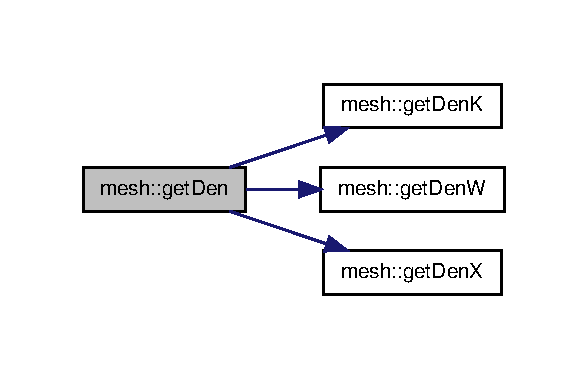
\includegraphics[width=282pt]{namespacemesh_a30c07812e0215d470457c9be91bb6b65_cgraph}
\end{center}
\end{figure}




Here is the caller graph for this function:
\nopagebreak
\begin{figure}[H]
\begin{center}
\leavevmode
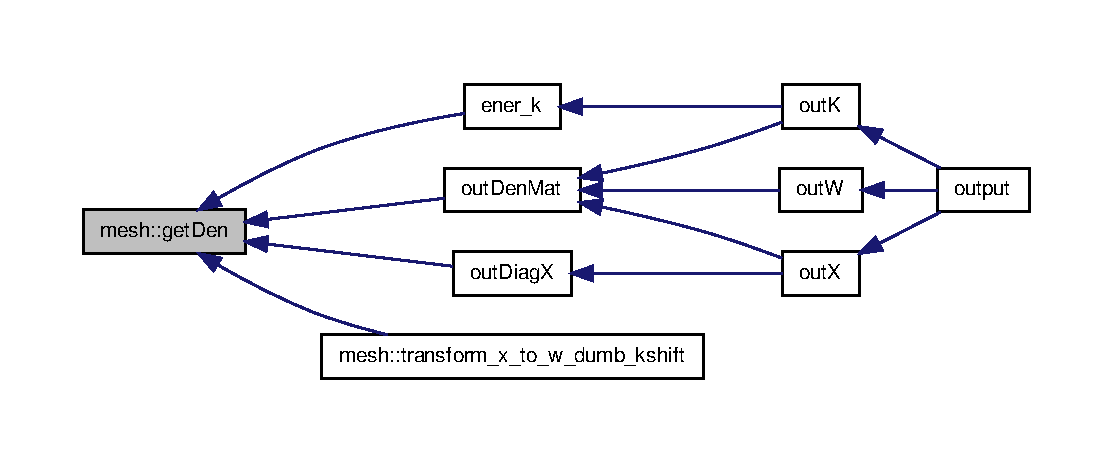
\includegraphics[width=400pt]{namespacemesh_a30c07812e0215d470457c9be91bb6b65_icgraph}
\end{center}
\end{figure}


\hypertarget{namespacemesh_af6c300cbff24f4eb25b428d822208430}{
\index{mesh@{mesh}!getDenDiagK@{getDenDiagK}}
\index{getDenDiagK@{getDenDiagK}!mesh@{mesh}}
\subsubsection[{getDenDiagK}]{\setlength{\rightskip}{0pt plus 5cm}complex$\ast$16 mesh::getDenDiagK (
\begin{DoxyParamCaption}
\item[{integer,intent(in)}]{ika}
\end{DoxyParamCaption}
)}}
\label{namespacemesh_af6c300cbff24f4eb25b428d822208430}


Definition at line 204 of file mesh.f90.



Here is the call graph for this function:\nopagebreak
\begin{figure}[H]
\begin{center}
\leavevmode
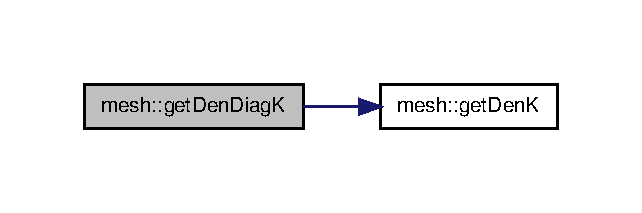
\includegraphics[width=308pt]{namespacemesh_af6c300cbff24f4eb25b428d822208430_cgraph}
\end{center}
\end{figure}


\hypertarget{namespacemesh_ab3a026a1c77fc428f9a77f0ee37b0616}{
\index{mesh@{mesh}!getDenEigens@{getDenEigens}}
\index{getDenEigens@{getDenEigens}!mesh@{mesh}}
\subsubsection[{getDenEigens}]{\setlength{\rightskip}{0pt plus 5cm}subroutine mesh::getDenEigens (
\begin{DoxyParamCaption}
\item[{complex$\ast$16,dimension(0:nxa-\/1),intent(out)}]{evals, }
\item[{complex$\ast$16,dimension(-\/nxa2:nxa2-\/1,-\/nxr2:nxr2-\/1),intent(out)}]{evecs}
\end{DoxyParamCaption}
)}}
\label{namespacemesh_ab3a026a1c77fc428f9a77f0ee37b0616}


Definition at line 345 of file mesh.f90.



Here is the call graph for this function:\nopagebreak
\begin{figure}[H]
\begin{center}
\leavevmode
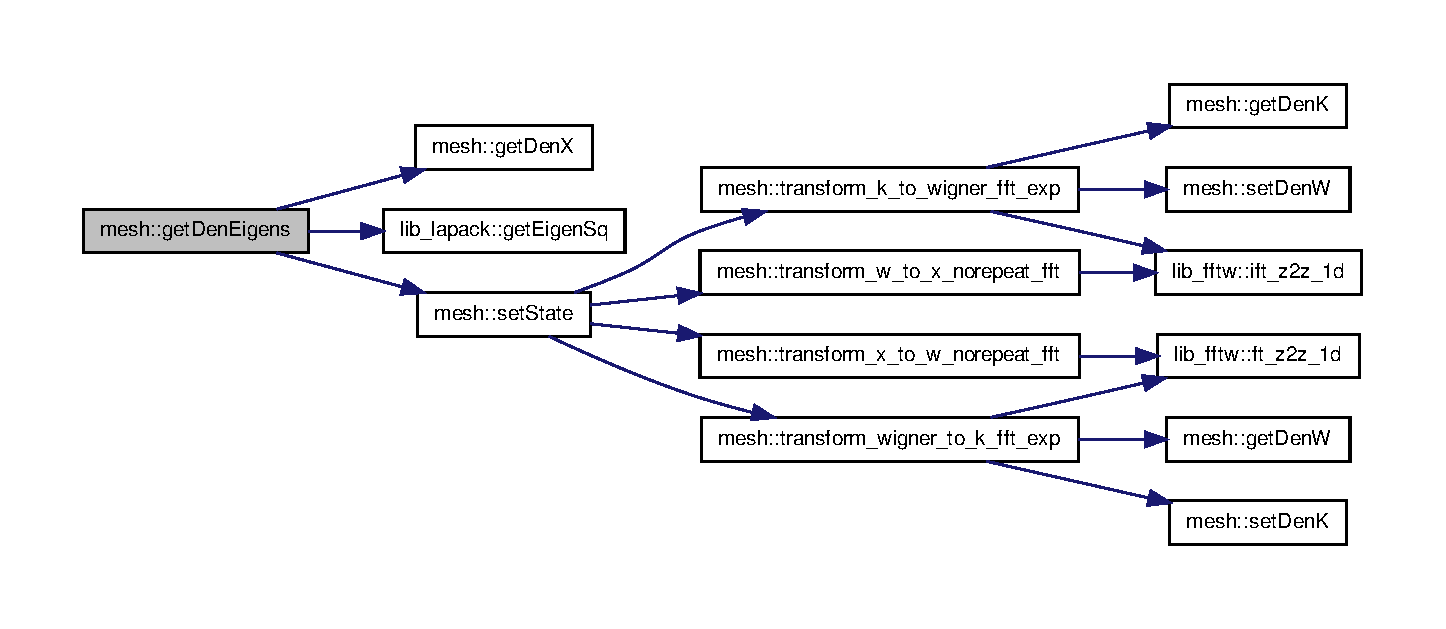
\includegraphics[width=400pt]{namespacemesh_ab3a026a1c77fc428f9a77f0ee37b0616_cgraph}
\end{center}
\end{figure}


\hypertarget{namespacemesh_ab4cd19eafd4df4568c11c147b12f952d}{
\index{mesh@{mesh}!getDenK@{getDenK}}
\index{getDenK@{getDenK}!mesh@{mesh}}
\subsubsection[{getDenK}]{\setlength{\rightskip}{0pt plus 5cm}complex$\ast$16 mesh::getDenK (
\begin{DoxyParamCaption}
\item[{integer,intent(in)}]{ikr, }
\item[{integer,intent(in)}]{ika}
\end{DoxyParamCaption}
)}}
\label{namespacemesh_ab4cd19eafd4df4568c11c147b12f952d}


Definition at line 319 of file mesh.f90.



Here is the caller graph for this function:
\nopagebreak
\begin{figure}[H]
\begin{center}
\leavevmode
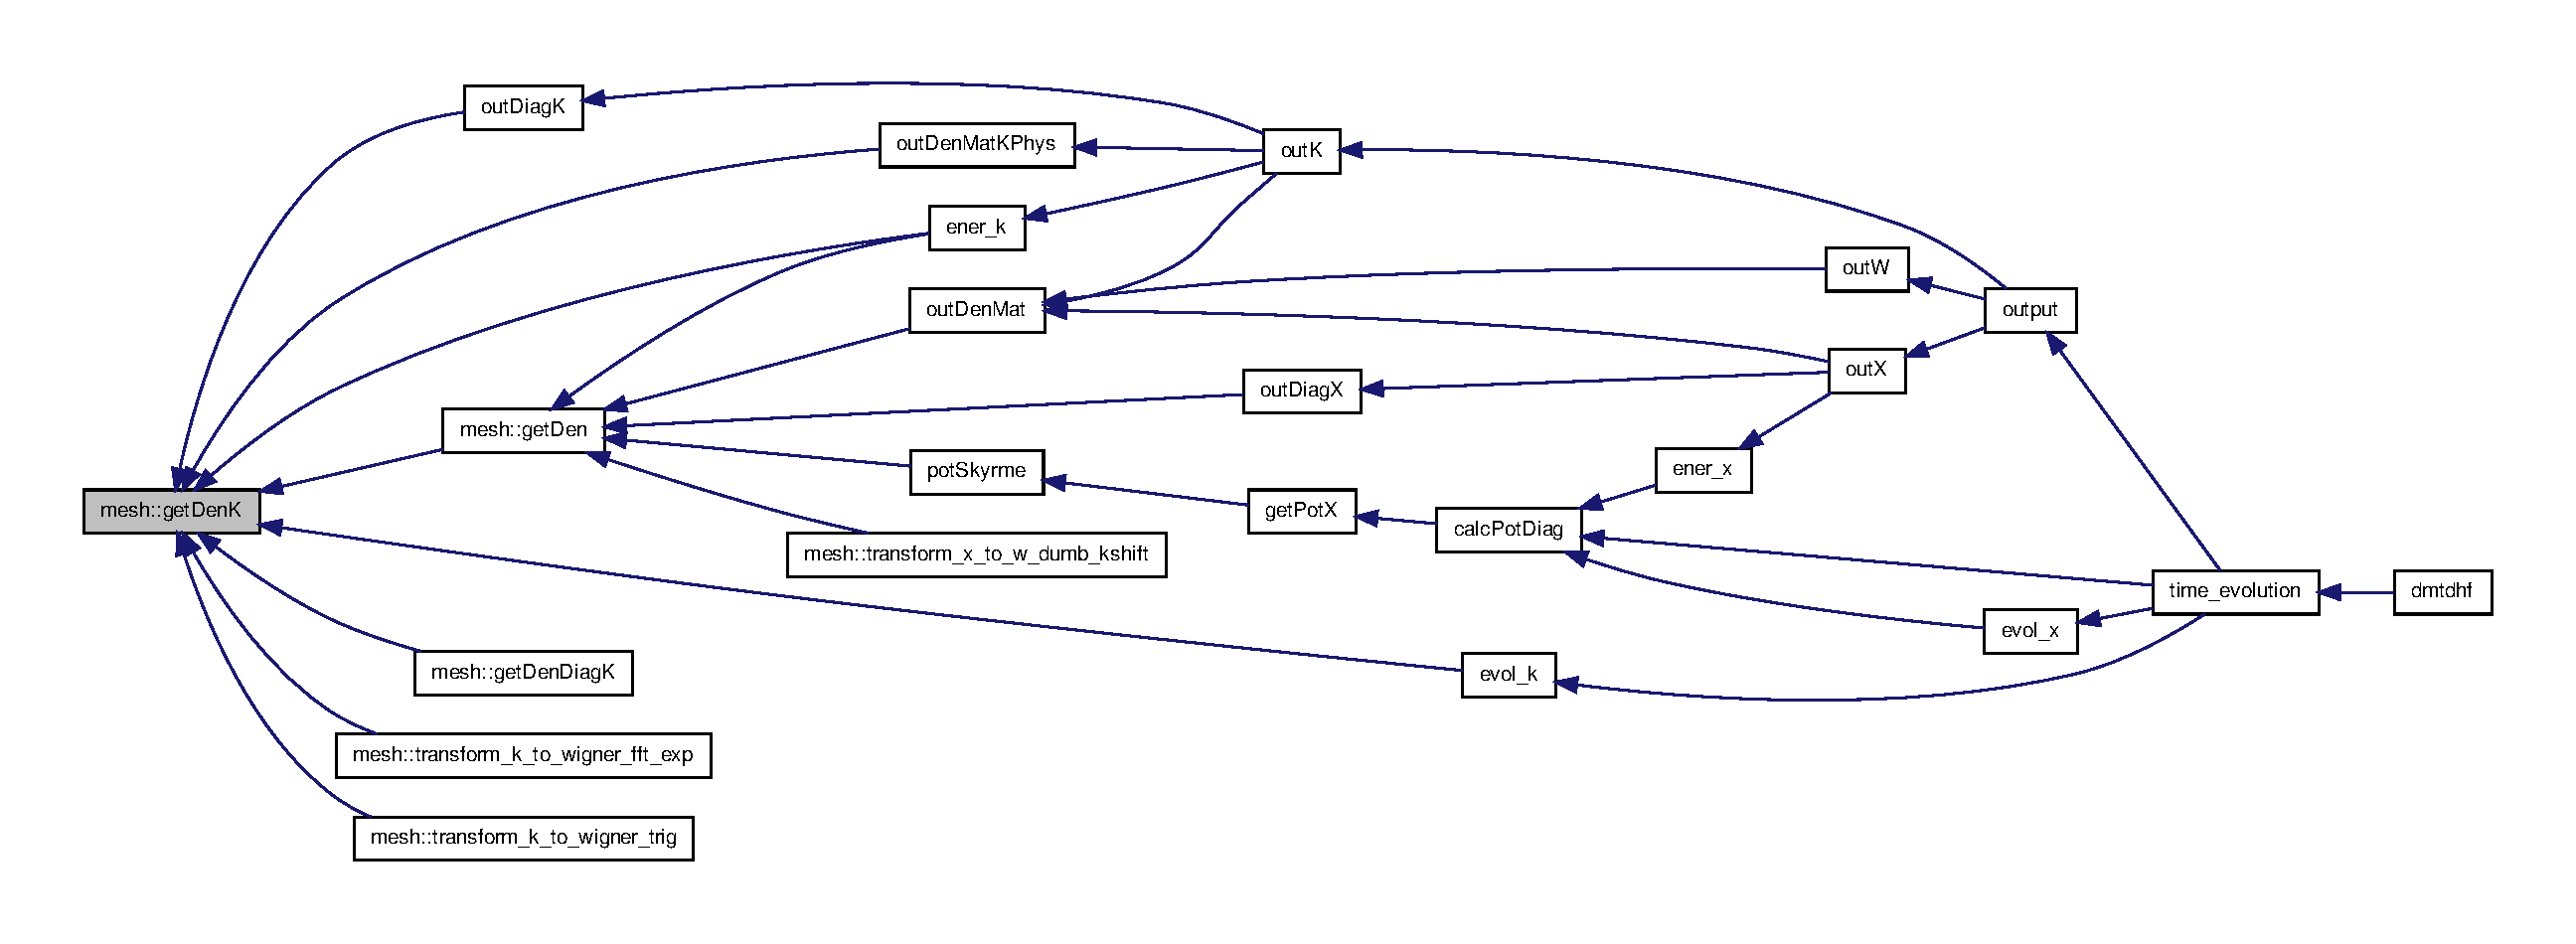
\includegraphics[width=400pt]{namespacemesh_ab4cd19eafd4df4568c11c147b12f952d_icgraph}
\end{center}
\end{figure}


\hypertarget{namespacemesh_a54f9135de9933edd2a34168c4e5ebfca}{
\index{mesh@{mesh}!getDenW@{getDenW}}
\index{getDenW@{getDenW}!mesh@{mesh}}
\subsubsection[{getDenW}]{\setlength{\rightskip}{0pt plus 5cm}complex$\ast$16 mesh::getDenW (
\begin{DoxyParamCaption}
\item[{integer,intent(in)}]{ixa, }
\item[{integer,intent(in)}]{ika}
\end{DoxyParamCaption}
)}}
\label{namespacemesh_a54f9135de9933edd2a34168c4e5ebfca}


Definition at line 290 of file mesh.f90.



Here is the caller graph for this function:
\nopagebreak
\begin{figure}[H]
\begin{center}
\leavevmode
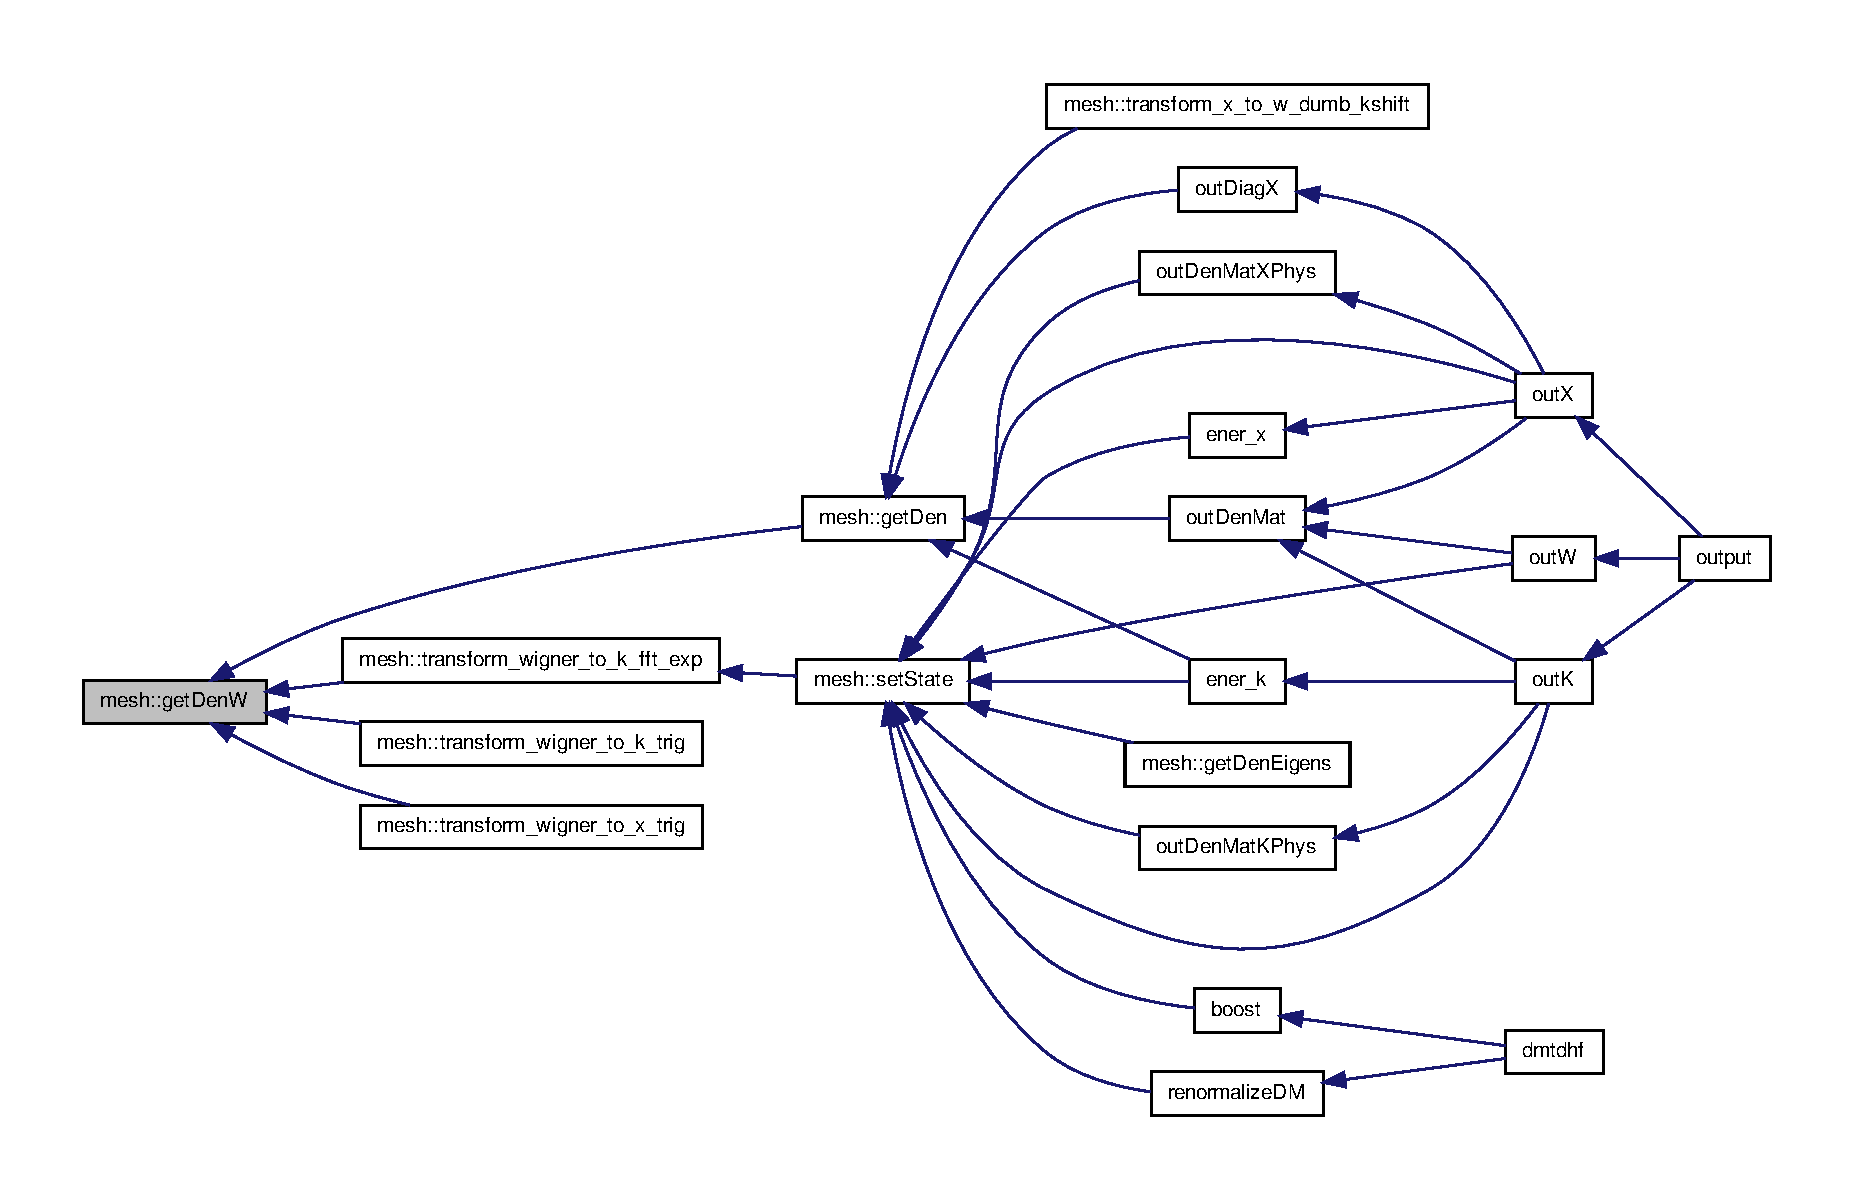
\includegraphics[width=400pt]{namespacemesh_a54f9135de9933edd2a34168c4e5ebfca_icgraph}
\end{center}
\end{figure}


\hypertarget{namespacemesh_a87ae177a6a4383943393f8efa7da0018}{
\index{mesh@{mesh}!getDenX@{getDenX}}
\index{getDenX@{getDenX}!mesh@{mesh}}
\subsubsection[{getDenX}]{\setlength{\rightskip}{0pt plus 5cm}complex$\ast$16 mesh::getDenX (
\begin{DoxyParamCaption}
\item[{integer,intent(in)}]{ixa, }
\item[{integer,intent(in)}]{ixr}
\end{DoxyParamCaption}
)}}
\label{namespacemesh_a87ae177a6a4383943393f8efa7da0018}


Definition at line 216 of file mesh.f90.



Here is the caller graph for this function:
\nopagebreak
\begin{figure}[H]
\begin{center}
\leavevmode
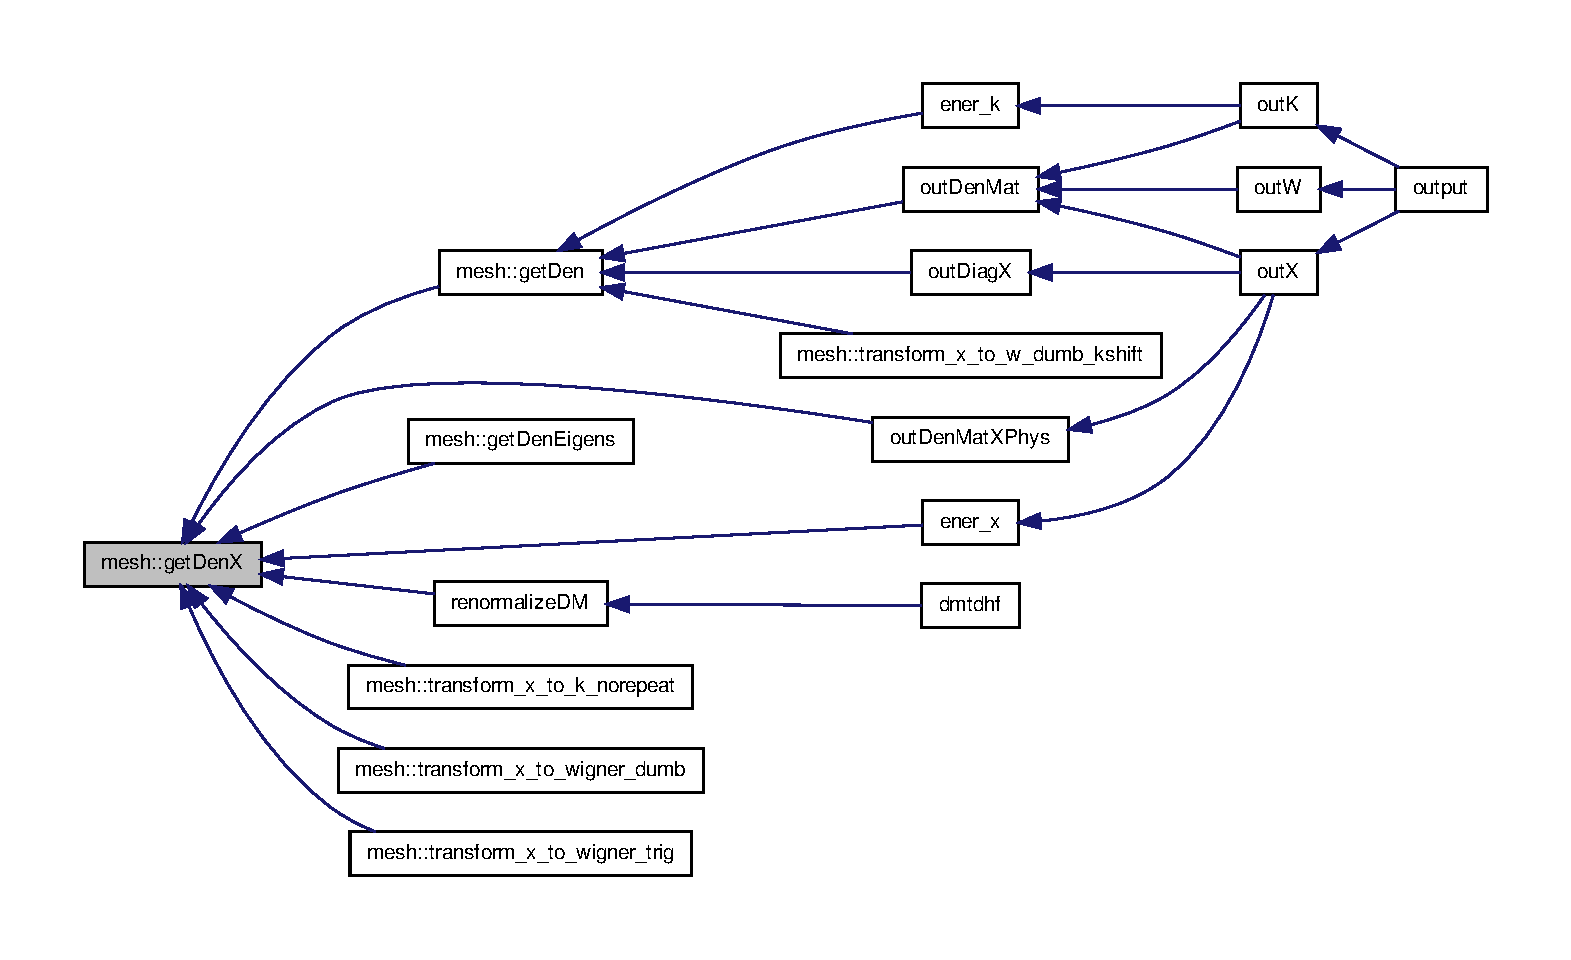
\includegraphics[width=400pt]{namespacemesh_a87ae177a6a4383943393f8efa7da0018_icgraph}
\end{center}
\end{figure}


\hypertarget{namespacemesh_ad1beeceb5580c23eb4fd6530573c395c}{
\index{mesh@{mesh}!getNearestIndexX@{getNearestIndexX}}
\index{getNearestIndexX@{getNearestIndexX}!mesh@{mesh}}
\subsubsection[{getNearestIndexX}]{\setlength{\rightskip}{0pt plus 5cm}integer mesh::getNearestIndexX (
\begin{DoxyParamCaption}
\item[{real (Long),intent(in)}]{xx}
\end{DoxyParamCaption}
)}}
\label{namespacemesh_ad1beeceb5580c23eb4fd6530573c395c}


Definition at line 82 of file mesh.f90.



Here is the caller graph for this function:
\nopagebreak
\begin{figure}[H]
\begin{center}
\leavevmode
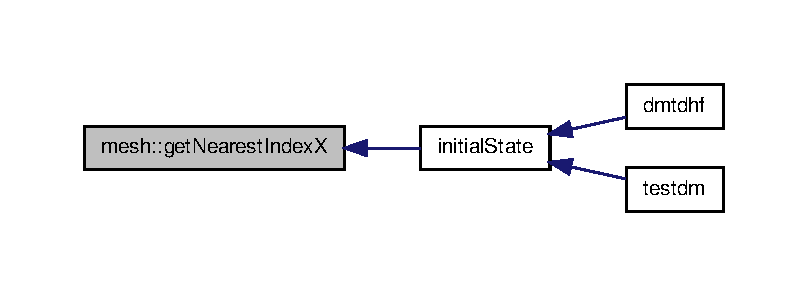
\includegraphics[width=388pt]{namespacemesh_ad1beeceb5580c23eb4fd6530573c395c_icgraph}
\end{center}
\end{figure}


\hypertarget{namespacemesh_a742012f09e48891eb9dd2a85601674a8}{
\index{mesh@{mesh}!initializeMesh@{initializeMesh}}
\index{initializeMesh@{initializeMesh}!mesh@{mesh}}
\subsubsection[{initializeMesh}]{\setlength{\rightskip}{0pt plus 5cm}subroutine mesh::initializeMesh (
\begin{DoxyParamCaption}
{}
\end{DoxyParamCaption}
)}}
\label{namespacemesh_a742012f09e48891eb9dd2a85601674a8}


Definition at line 106 of file mesh.f90.



Here is the caller graph for this function:
\nopagebreak
\begin{figure}[H]
\begin{center}
\leavevmode
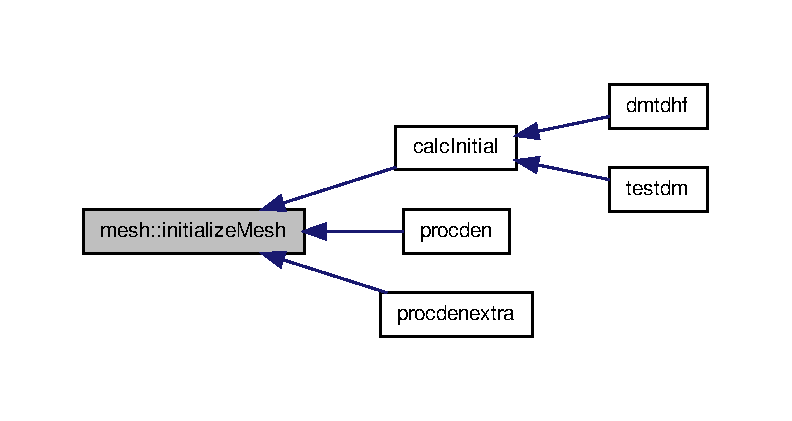
\includegraphics[width=380pt]{namespacemesh_a742012f09e48891eb9dd2a85601674a8_icgraph}
\end{center}
\end{figure}


\hypertarget{namespacemesh_abf02ca88d15c266099562e937ee507e4}{
\index{mesh@{mesh}!mesh\_\-reflectLR@{mesh\_\-reflectLR}}
\index{mesh\_\-reflectLR@{mesh\_\-reflectLR}!mesh@{mesh}}
\subsubsection[{mesh\_\-reflectLR}]{\setlength{\rightskip}{0pt plus 5cm}subroutine mesh::mesh\_\-reflectLR (
\begin{DoxyParamCaption}
{}
\end{DoxyParamCaption}
)}}
\label{namespacemesh_abf02ca88d15c266099562e937ee507e4}


Definition at line 228 of file mesh.f90.



Here is the caller graph for this function:
\nopagebreak
\begin{figure}[H]
\begin{center}
\leavevmode
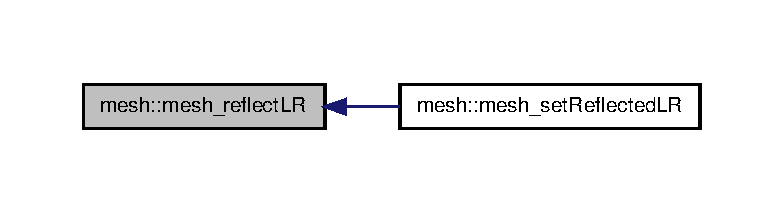
\includegraphics[width=376pt]{namespacemesh_abf02ca88d15c266099562e937ee507e4_icgraph}
\end{center}
\end{figure}


\hypertarget{namespacemesh_ac5a0f33502939ba9fae215e203d895f0}{
\index{mesh@{mesh}!mesh\_\-setReflectedLR@{mesh\_\-setReflectedLR}}
\index{mesh\_\-setReflectedLR@{mesh\_\-setReflectedLR}!mesh@{mesh}}
\subsubsection[{mesh\_\-setReflectedLR}]{\setlength{\rightskip}{0pt plus 5cm}subroutine mesh::mesh\_\-setReflectedLR (
\begin{DoxyParamCaption}
\item[{logical,intent(in)}]{reflect}
\end{DoxyParamCaption}
)}}
\label{namespacemesh_ac5a0f33502939ba9fae215e203d895f0}


Definition at line 264 of file mesh.f90.



Here is the call graph for this function:\nopagebreak
\begin{figure}[H]
\begin{center}
\leavevmode
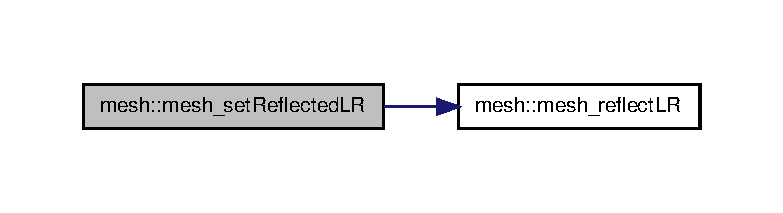
\includegraphics[width=376pt]{namespacemesh_ac5a0f33502939ba9fae215e203d895f0_cgraph}
\end{center}
\end{figure}


\hypertarget{namespacemesh_a16330a30f3f56c2944ef63240c049ee7}{
\index{mesh@{mesh}!setDenK@{setDenK}}
\index{setDenK@{setDenK}!mesh@{mesh}}
\subsubsection[{setDenK}]{\setlength{\rightskip}{0pt plus 5cm}subroutine mesh::setDenK (
\begin{DoxyParamCaption}
\item[{integer,intent(in)}]{ikr, }
\item[{integer,intent(in)}]{ika, }
\item[{complex$\ast$16,intent(in)}]{val}
\end{DoxyParamCaption}
)}}
\label{namespacemesh_a16330a30f3f56c2944ef63240c049ee7}


Definition at line 331 of file mesh.f90.



Here is the caller graph for this function:
\nopagebreak
\begin{figure}[H]
\begin{center}
\leavevmode
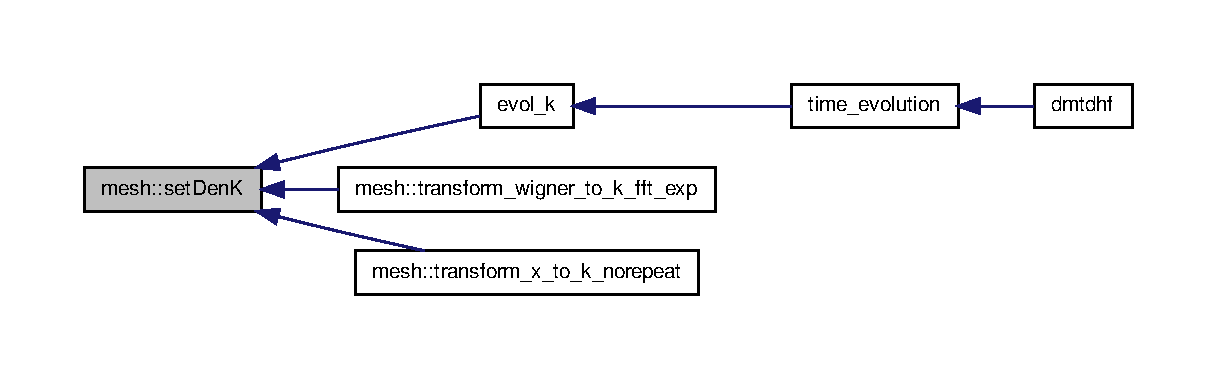
\includegraphics[width=400pt]{namespacemesh_a16330a30f3f56c2944ef63240c049ee7_icgraph}
\end{center}
\end{figure}


\hypertarget{namespacemesh_a7e79531a47425f91c6ac0921fc2203ed}{
\index{mesh@{mesh}!setDenW@{setDenW}}
\index{setDenW@{setDenW}!mesh@{mesh}}
\subsubsection[{setDenW}]{\setlength{\rightskip}{0pt plus 5cm}subroutine mesh::setDenW (
\begin{DoxyParamCaption}
\item[{integer,intent(in)}]{ixa, }
\item[{integer,intent(in)}]{ika, }
\item[{complex$\ast$16,intent(in)}]{this\_\-value}
\end{DoxyParamCaption}
)}}
\label{namespacemesh_a7e79531a47425f91c6ac0921fc2203ed}


Definition at line 307 of file mesh.f90.



Here is the caller graph for this function:
\nopagebreak
\begin{figure}[H]
\begin{center}
\leavevmode
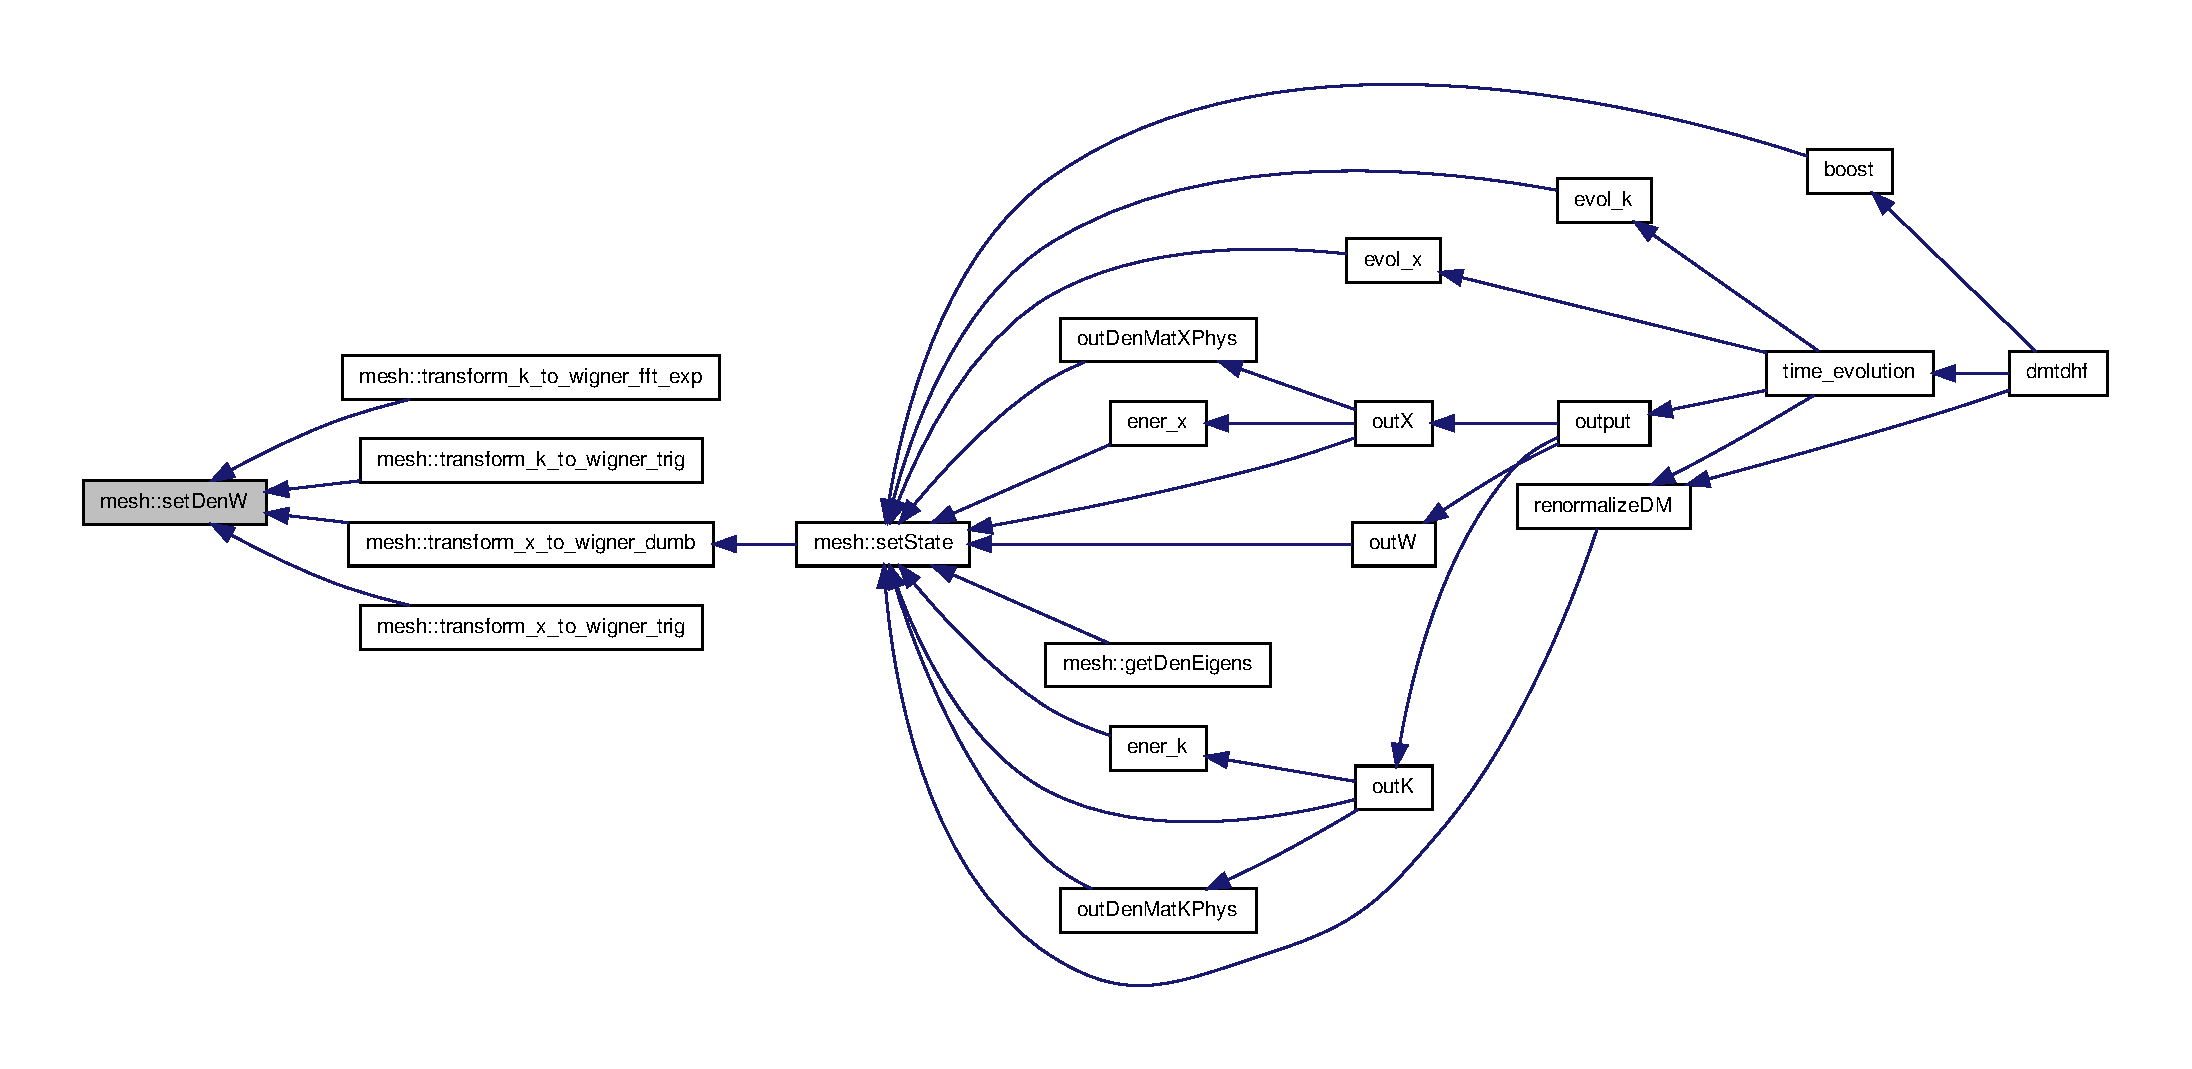
\includegraphics[width=400pt]{namespacemesh_a7e79531a47425f91c6ac0921fc2203ed_icgraph}
\end{center}
\end{figure}


\hypertarget{namespacemesh_a7f55b8b4c3e045f04553b292c323b43a}{
\index{mesh@{mesh}!setDenX@{setDenX}}
\index{setDenX@{setDenX}!mesh@{mesh}}
\subsubsection[{setDenX}]{\setlength{\rightskip}{0pt plus 5cm}subroutine mesh::setDenX (
\begin{DoxyParamCaption}
\item[{integer,intent(in)}]{ixa, }
\item[{integer,intent(in)}]{ixr, }
\item[{complex$\ast$16,intent(in)}]{value}
\end{DoxyParamCaption}
)}}
\label{namespacemesh_a7f55b8b4c3e045f04553b292c323b43a}


Definition at line 277 of file mesh.f90.



Here is the caller graph for this function:
\nopagebreak
\begin{figure}[H]
\begin{center}
\leavevmode
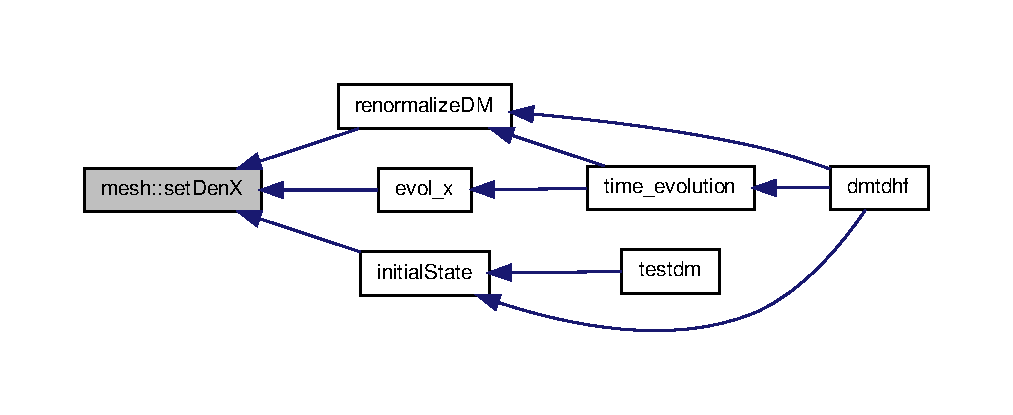
\includegraphics[width=400pt]{namespacemesh_a7f55b8b4c3e045f04553b292c323b43a_icgraph}
\end{center}
\end{figure}


\hypertarget{namespacemesh_aef51df23ee69f610420b25672a2da3ef}{
\index{mesh@{mesh}!setState@{setState}}
\index{setState@{setState}!mesh@{mesh}}
\subsubsection[{setState}]{\setlength{\rightskip}{0pt plus 5cm}subroutine mesh::setState (
\begin{DoxyParamCaption}
\item[{integer,intent(in)}]{state}
\end{DoxyParamCaption}
)}}
\label{namespacemesh_aef51df23ee69f610420b25672a2da3ef}


Definition at line 376 of file mesh.f90.



Here is the call graph for this function:\nopagebreak
\begin{figure}[H]
\begin{center}
\leavevmode
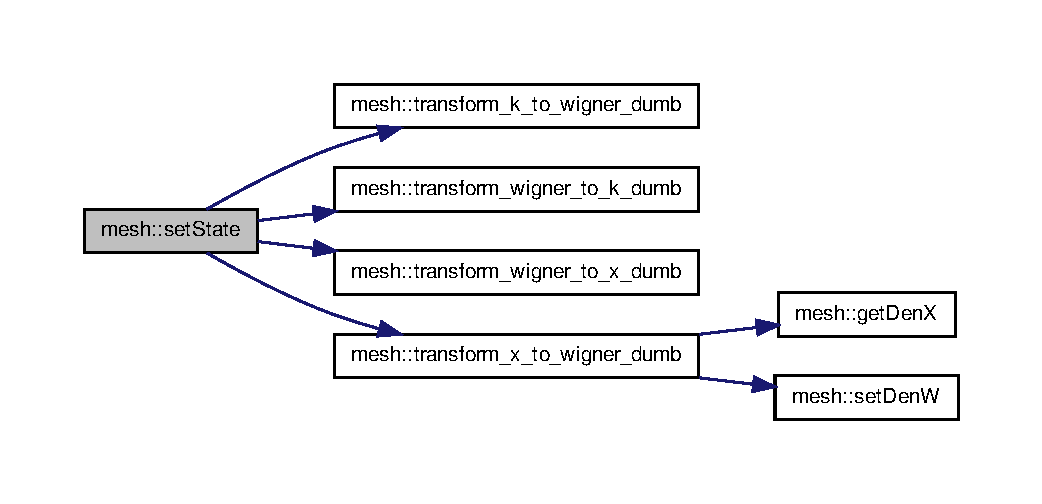
\includegraphics[width=400pt]{namespacemesh_aef51df23ee69f610420b25672a2da3ef_cgraph}
\end{center}
\end{figure}




Here is the caller graph for this function:
\nopagebreak
\begin{figure}[H]
\begin{center}
\leavevmode
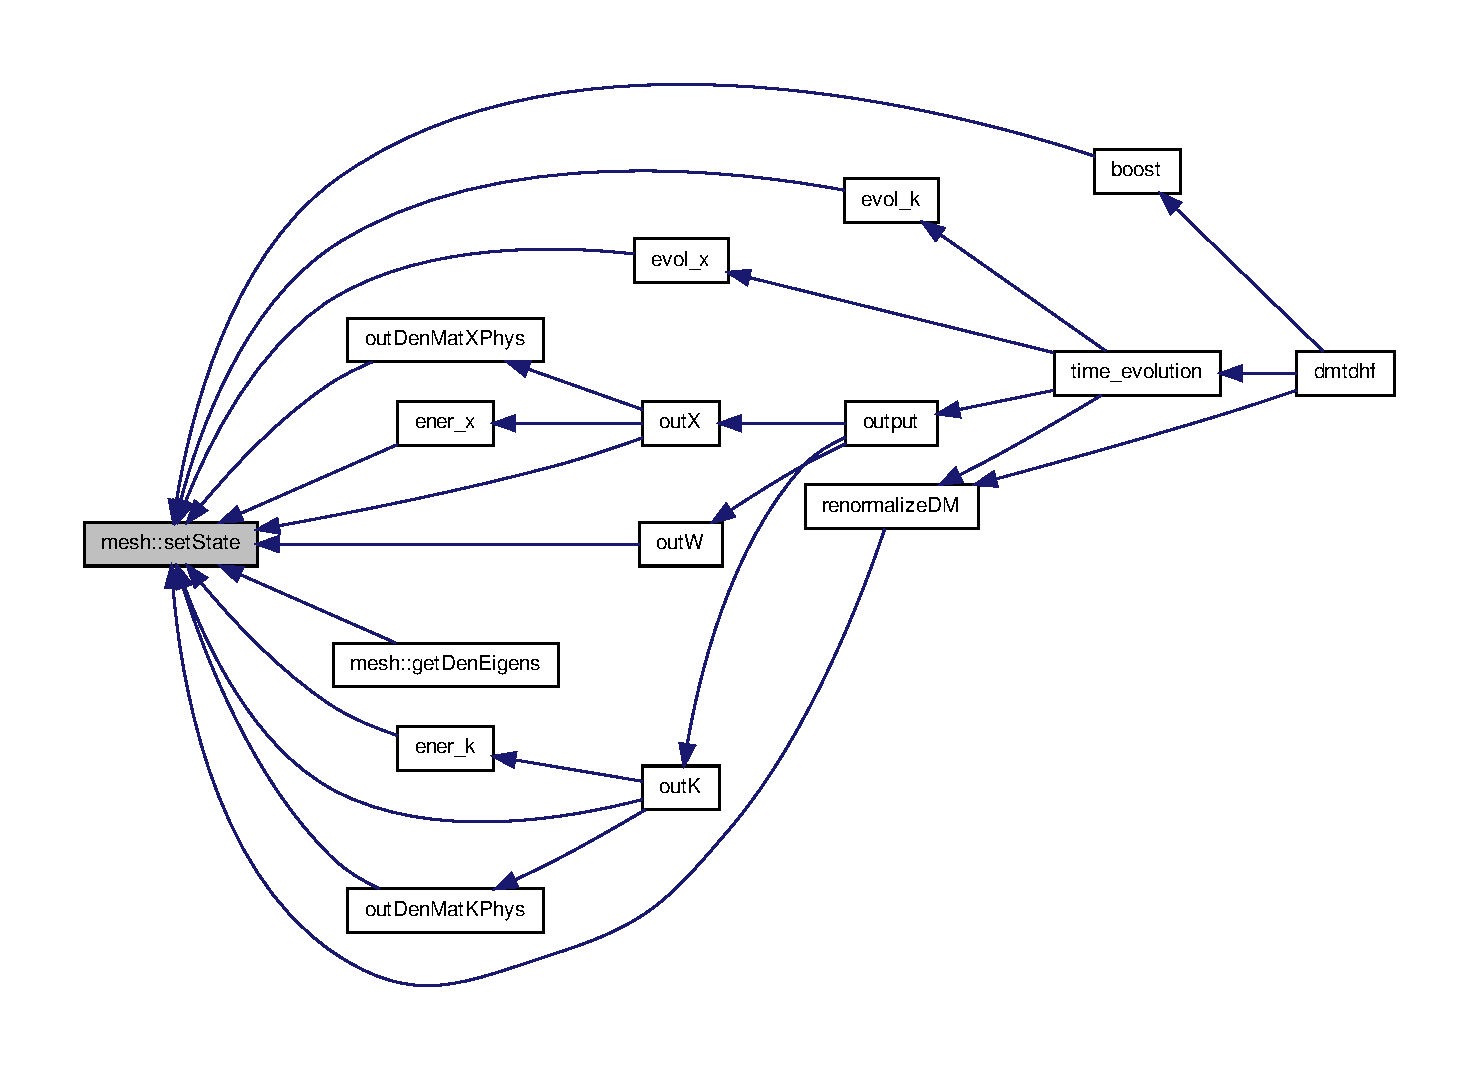
\includegraphics[width=400pt]{namespacemesh_aef51df23ee69f610420b25672a2da3ef_icgraph}
\end{center}
\end{figure}


\hypertarget{namespacemesh_a10655d39a753ec023b2c6b9d36db4663}{
\index{mesh@{mesh}!transform\_\-k\_\-to\_\-wigner\_\-dumb@{transform\_\-k\_\-to\_\-wigner\_\-dumb}}
\index{transform\_\-k\_\-to\_\-wigner\_\-dumb@{transform\_\-k\_\-to\_\-wigner\_\-dumb}!mesh@{mesh}}
\subsubsection[{transform\_\-k\_\-to\_\-wigner\_\-dumb}]{\setlength{\rightskip}{0pt plus 5cm}subroutine mesh::transform\_\-k\_\-to\_\-wigner\_\-dumb (
\begin{DoxyParamCaption}
{}
\end{DoxyParamCaption}
)}}
\label{namespacemesh_a10655d39a753ec023b2c6b9d36db4663}


Definition at line 961 of file mesh.f90.



Here is the caller graph for this function:
\nopagebreak
\begin{figure}[H]
\begin{center}
\leavevmode
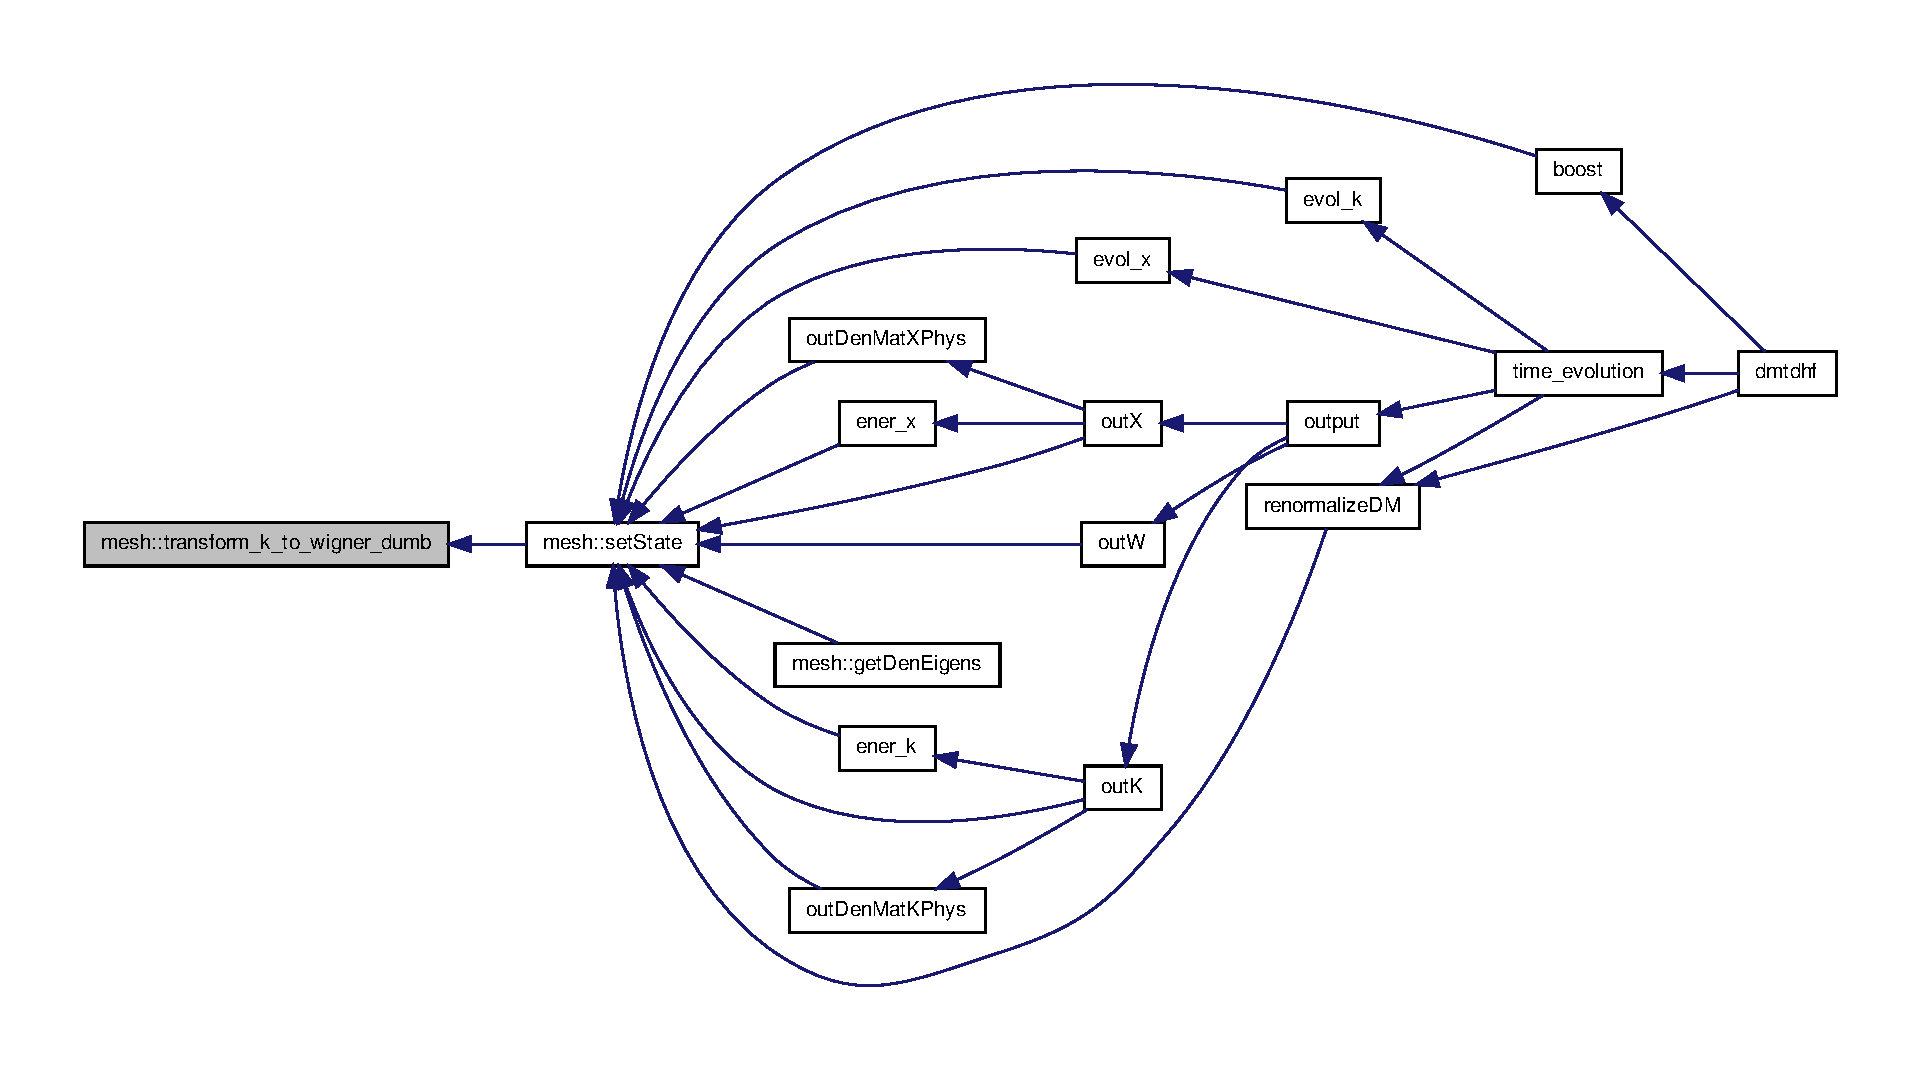
\includegraphics[width=400pt]{namespacemesh_a10655d39a753ec023b2c6b9d36db4663_icgraph}
\end{center}
\end{figure}


\hypertarget{namespacemesh_a6d0133c6c55c6bfd1929d28d4e48e2d6}{
\index{mesh@{mesh}!transform\_\-k\_\-to\_\-wigner\_\-fft\_\-exp@{transform\_\-k\_\-to\_\-wigner\_\-fft\_\-exp}}
\index{transform\_\-k\_\-to\_\-wigner\_\-fft\_\-exp@{transform\_\-k\_\-to\_\-wigner\_\-fft\_\-exp}!mesh@{mesh}}
\subsubsection[{transform\_\-k\_\-to\_\-wigner\_\-fft\_\-exp}]{\setlength{\rightskip}{0pt plus 5cm}subroutine mesh::transform\_\-k\_\-to\_\-wigner\_\-fft\_\-exp (
\begin{DoxyParamCaption}
{}
\end{DoxyParamCaption}
)}}
\label{namespacemesh_a6d0133c6c55c6bfd1929d28d4e48e2d6}


Definition at line 1001 of file mesh.f90.



Here is the call graph for this function:\nopagebreak
\begin{figure}[H]
\begin{center}
\leavevmode
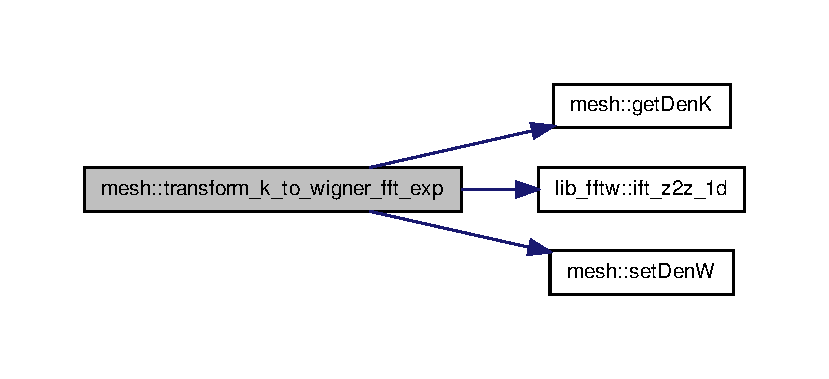
\includegraphics[width=398pt]{namespacemesh_a6d0133c6c55c6bfd1929d28d4e48e2d6_cgraph}
\end{center}
\end{figure}


\hypertarget{namespacemesh_ad6c116013ec5d5d4b1e8298749ffa481}{
\index{mesh@{mesh}!transform\_\-k\_\-to\_\-wigner\_\-trig@{transform\_\-k\_\-to\_\-wigner\_\-trig}}
\index{transform\_\-k\_\-to\_\-wigner\_\-trig@{transform\_\-k\_\-to\_\-wigner\_\-trig}!mesh@{mesh}}
\subsubsection[{transform\_\-k\_\-to\_\-wigner\_\-trig}]{\setlength{\rightskip}{0pt plus 5cm}subroutine mesh::transform\_\-k\_\-to\_\-wigner\_\-trig (
\begin{DoxyParamCaption}
{}
\end{DoxyParamCaption}
)}}
\label{namespacemesh_ad6c116013ec5d5d4b1e8298749ffa481}


Definition at line 800 of file mesh.f90.



Here is the call graph for this function:\nopagebreak
\begin{figure}[H]
\begin{center}
\leavevmode
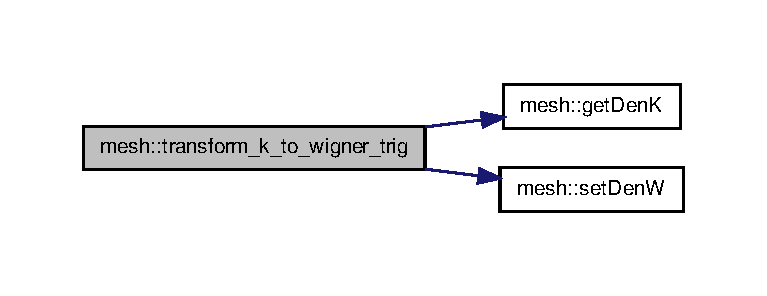
\includegraphics[width=368pt]{namespacemesh_ad6c116013ec5d5d4b1e8298749ffa481_cgraph}
\end{center}
\end{figure}


\hypertarget{namespacemesh_accd03020a8a261cbf51d9642814db3cb}{
\index{mesh@{mesh}!transform\_\-w\_\-to\_\-k\_\-norepeat@{transform\_\-w\_\-to\_\-k\_\-norepeat}}
\index{transform\_\-w\_\-to\_\-k\_\-norepeat@{transform\_\-w\_\-to\_\-k\_\-norepeat}!mesh@{mesh}}
\subsubsection[{transform\_\-w\_\-to\_\-k\_\-norepeat}]{\setlength{\rightskip}{0pt plus 5cm}subroutine mesh::transform\_\-w\_\-to\_\-k\_\-norepeat (
\begin{DoxyParamCaption}
{}
\end{DoxyParamCaption}
)}}
\label{namespacemesh_accd03020a8a261cbf51d9642814db3cb}


Definition at line 1313 of file mesh.f90.

\hypertarget{namespacemesh_af0c42421bd8b5b74a00094f639c4f7c7}{
\index{mesh@{mesh}!transform\_\-w\_\-to\_\-x\_\-norepeat\_\-fft@{transform\_\-w\_\-to\_\-x\_\-norepeat\_\-fft}}
\index{transform\_\-w\_\-to\_\-x\_\-norepeat\_\-fft@{transform\_\-w\_\-to\_\-x\_\-norepeat\_\-fft}!mesh@{mesh}}
\subsubsection[{transform\_\-w\_\-to\_\-x\_\-norepeat\_\-fft}]{\setlength{\rightskip}{0pt plus 5cm}subroutine mesh::transform\_\-w\_\-to\_\-x\_\-norepeat\_\-fft (
\begin{DoxyParamCaption}
{}
\end{DoxyParamCaption}
)}}
\label{namespacemesh_af0c42421bd8b5b74a00094f639c4f7c7}


Definition at line 603 of file mesh.f90.



Here is the call graph for this function:\nopagebreak
\begin{figure}[H]
\begin{center}
\leavevmode
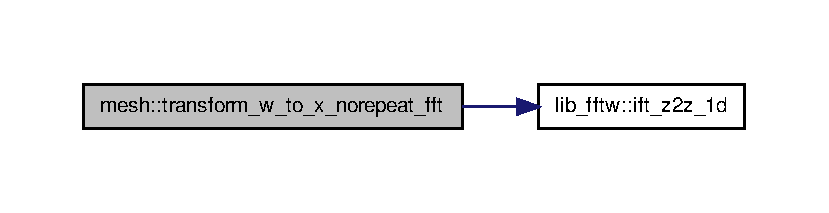
\includegraphics[width=398pt]{namespacemesh_af0c42421bd8b5b74a00094f639c4f7c7_cgraph}
\end{center}
\end{figure}


\hypertarget{namespacemesh_ac641e03ceee3eaba6206a6e3b03db6af}{
\index{mesh@{mesh}!transform\_\-w\_\-to\_\-x\_\-norepeat\_\-fft\_\-bad@{transform\_\-w\_\-to\_\-x\_\-norepeat\_\-fft\_\-bad}}
\index{transform\_\-w\_\-to\_\-x\_\-norepeat\_\-fft\_\-bad@{transform\_\-w\_\-to\_\-x\_\-norepeat\_\-fft\_\-bad}!mesh@{mesh}}
\subsubsection[{transform\_\-w\_\-to\_\-x\_\-norepeat\_\-fft\_\-bad}]{\setlength{\rightskip}{0pt plus 5cm}subroutine mesh::transform\_\-w\_\-to\_\-x\_\-norepeat\_\-fft\_\-bad (
\begin{DoxyParamCaption}
{}
\end{DoxyParamCaption}
)}}
\label{namespacemesh_ac641e03ceee3eaba6206a6e3b03db6af}


Definition at line 648 of file mesh.f90.



Here is the call graph for this function:\nopagebreak
\begin{figure}[H]
\begin{center}
\leavevmode
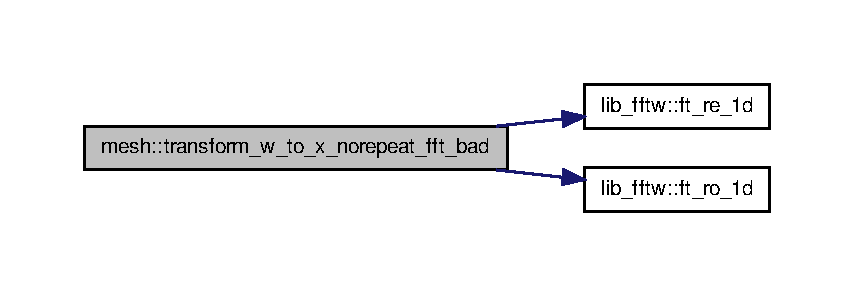
\includegraphics[width=400pt]{namespacemesh_ac641e03ceee3eaba6206a6e3b03db6af_cgraph}
\end{center}
\end{figure}


\hypertarget{namespacemesh_ad10642a5ceb6239ab5dbf2124a221b45}{
\index{mesh@{mesh}!transform\_\-wigner\_\-to\_\-k\_\-dumb@{transform\_\-wigner\_\-to\_\-k\_\-dumb}}
\index{transform\_\-wigner\_\-to\_\-k\_\-dumb@{transform\_\-wigner\_\-to\_\-k\_\-dumb}!mesh@{mesh}}
\subsubsection[{transform\_\-wigner\_\-to\_\-k\_\-dumb}]{\setlength{\rightskip}{0pt plus 5cm}subroutine mesh::transform\_\-wigner\_\-to\_\-k\_\-dumb (
\begin{DoxyParamCaption}
{}
\end{DoxyParamCaption}
)}}
\label{namespacemesh_ad10642a5ceb6239ab5dbf2124a221b45}


Definition at line 874 of file mesh.f90.



Here is the caller graph for this function:
\nopagebreak
\begin{figure}[H]
\begin{center}
\leavevmode
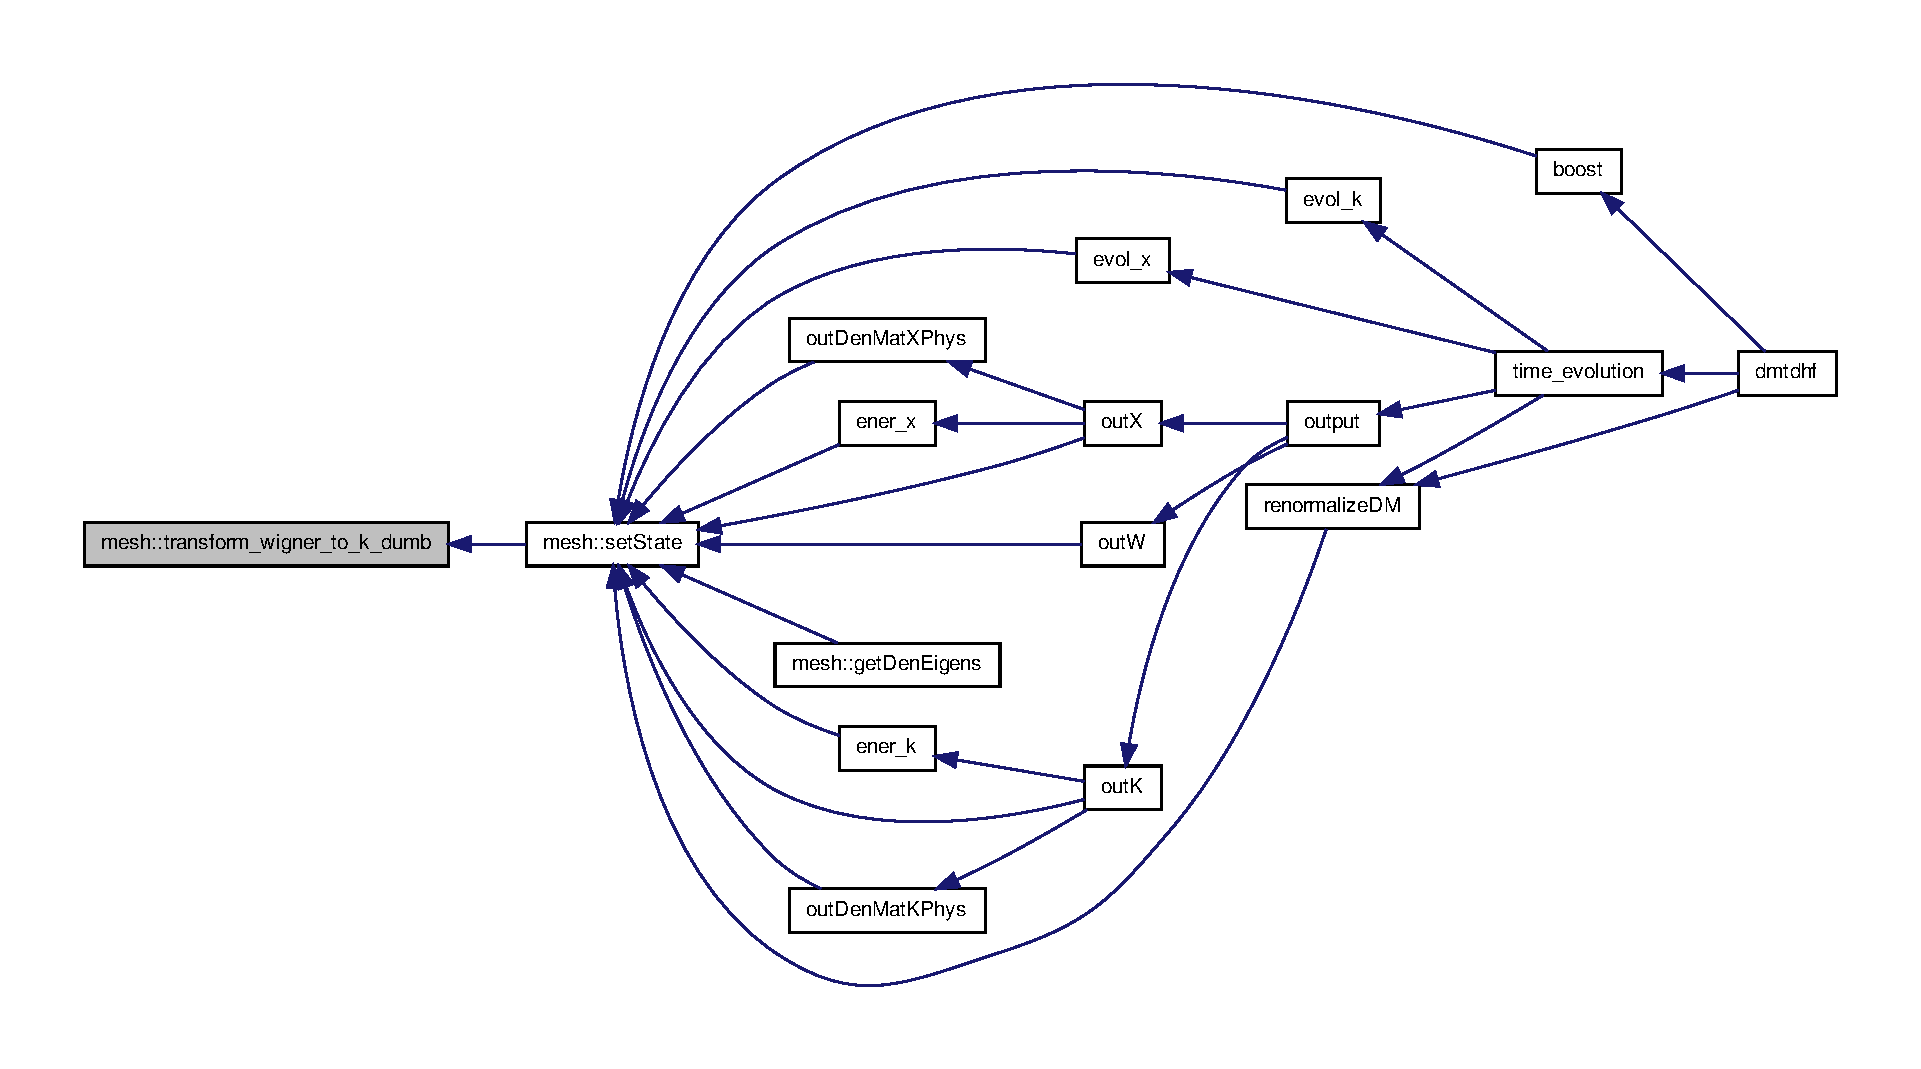
\includegraphics[width=400pt]{namespacemesh_ad10642a5ceb6239ab5dbf2124a221b45_icgraph}
\end{center}
\end{figure}


\hypertarget{namespacemesh_ac76ffd458b6317525fb12c63498439e4}{
\index{mesh@{mesh}!transform\_\-wigner\_\-to\_\-k\_\-fft\_\-exp@{transform\_\-wigner\_\-to\_\-k\_\-fft\_\-exp}}
\index{transform\_\-wigner\_\-to\_\-k\_\-fft\_\-exp@{transform\_\-wigner\_\-to\_\-k\_\-fft\_\-exp}!mesh@{mesh}}
\subsubsection[{transform\_\-wigner\_\-to\_\-k\_\-fft\_\-exp}]{\setlength{\rightskip}{0pt plus 5cm}subroutine mesh::transform\_\-wigner\_\-to\_\-k\_\-fft\_\-exp (
\begin{DoxyParamCaption}
{}
\end{DoxyParamCaption}
)}}
\label{namespacemesh_ac76ffd458b6317525fb12c63498439e4}


Definition at line 919 of file mesh.f90.



Here is the call graph for this function:\nopagebreak
\begin{figure}[H]
\begin{center}
\leavevmode
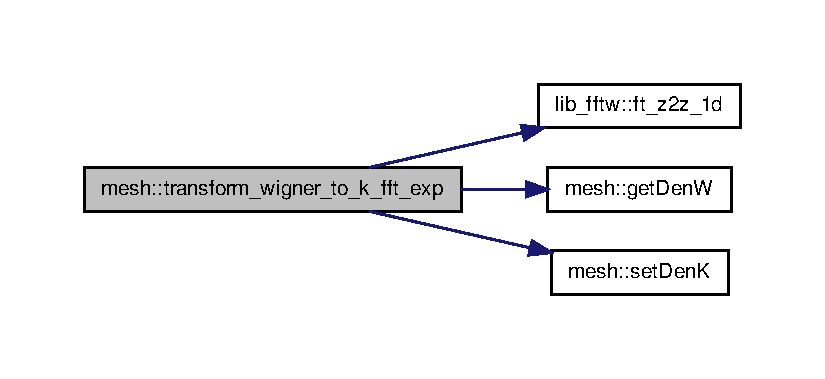
\includegraphics[width=396pt]{namespacemesh_ac76ffd458b6317525fb12c63498439e4_cgraph}
\end{center}
\end{figure}


\hypertarget{namespacemesh_affe8a5fb2705abf8f10cbac993ae66ff}{
\index{mesh@{mesh}!transform\_\-wigner\_\-to\_\-k\_\-trig@{transform\_\-wigner\_\-to\_\-k\_\-trig}}
\index{transform\_\-wigner\_\-to\_\-k\_\-trig@{transform\_\-wigner\_\-to\_\-k\_\-trig}!mesh@{mesh}}
\subsubsection[{transform\_\-wigner\_\-to\_\-k\_\-trig}]{\setlength{\rightskip}{0pt plus 5cm}subroutine mesh::transform\_\-wigner\_\-to\_\-k\_\-trig (
\begin{DoxyParamCaption}
{}
\end{DoxyParamCaption}
)}}
\label{namespacemesh_affe8a5fb2705abf8f10cbac993ae66ff}


Definition at line 850 of file mesh.f90.



Here is the call graph for this function:\nopagebreak
\begin{figure}[H]
\begin{center}
\leavevmode
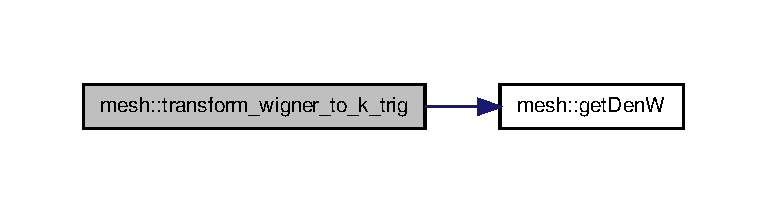
\includegraphics[width=368pt]{namespacemesh_affe8a5fb2705abf8f10cbac993ae66ff_cgraph}
\end{center}
\end{figure}


\hypertarget{namespacemesh_aee41613b43ab6e2f5a715e21c4227f4c}{
\index{mesh@{mesh}!transform\_\-wigner\_\-to\_\-x\_\-dumb@{transform\_\-wigner\_\-to\_\-x\_\-dumb}}
\index{transform\_\-wigner\_\-to\_\-x\_\-dumb@{transform\_\-wigner\_\-to\_\-x\_\-dumb}!mesh@{mesh}}
\subsubsection[{transform\_\-wigner\_\-to\_\-x\_\-dumb}]{\setlength{\rightskip}{0pt plus 5cm}subroutine mesh::transform\_\-wigner\_\-to\_\-x\_\-dumb (
\begin{DoxyParamCaption}
{}
\end{DoxyParamCaption}
)}}
\label{namespacemesh_aee41613b43ab6e2f5a715e21c4227f4c}


Definition at line 762 of file mesh.f90.



Here is the caller graph for this function:
\nopagebreak
\begin{figure}[H]
\begin{center}
\leavevmode
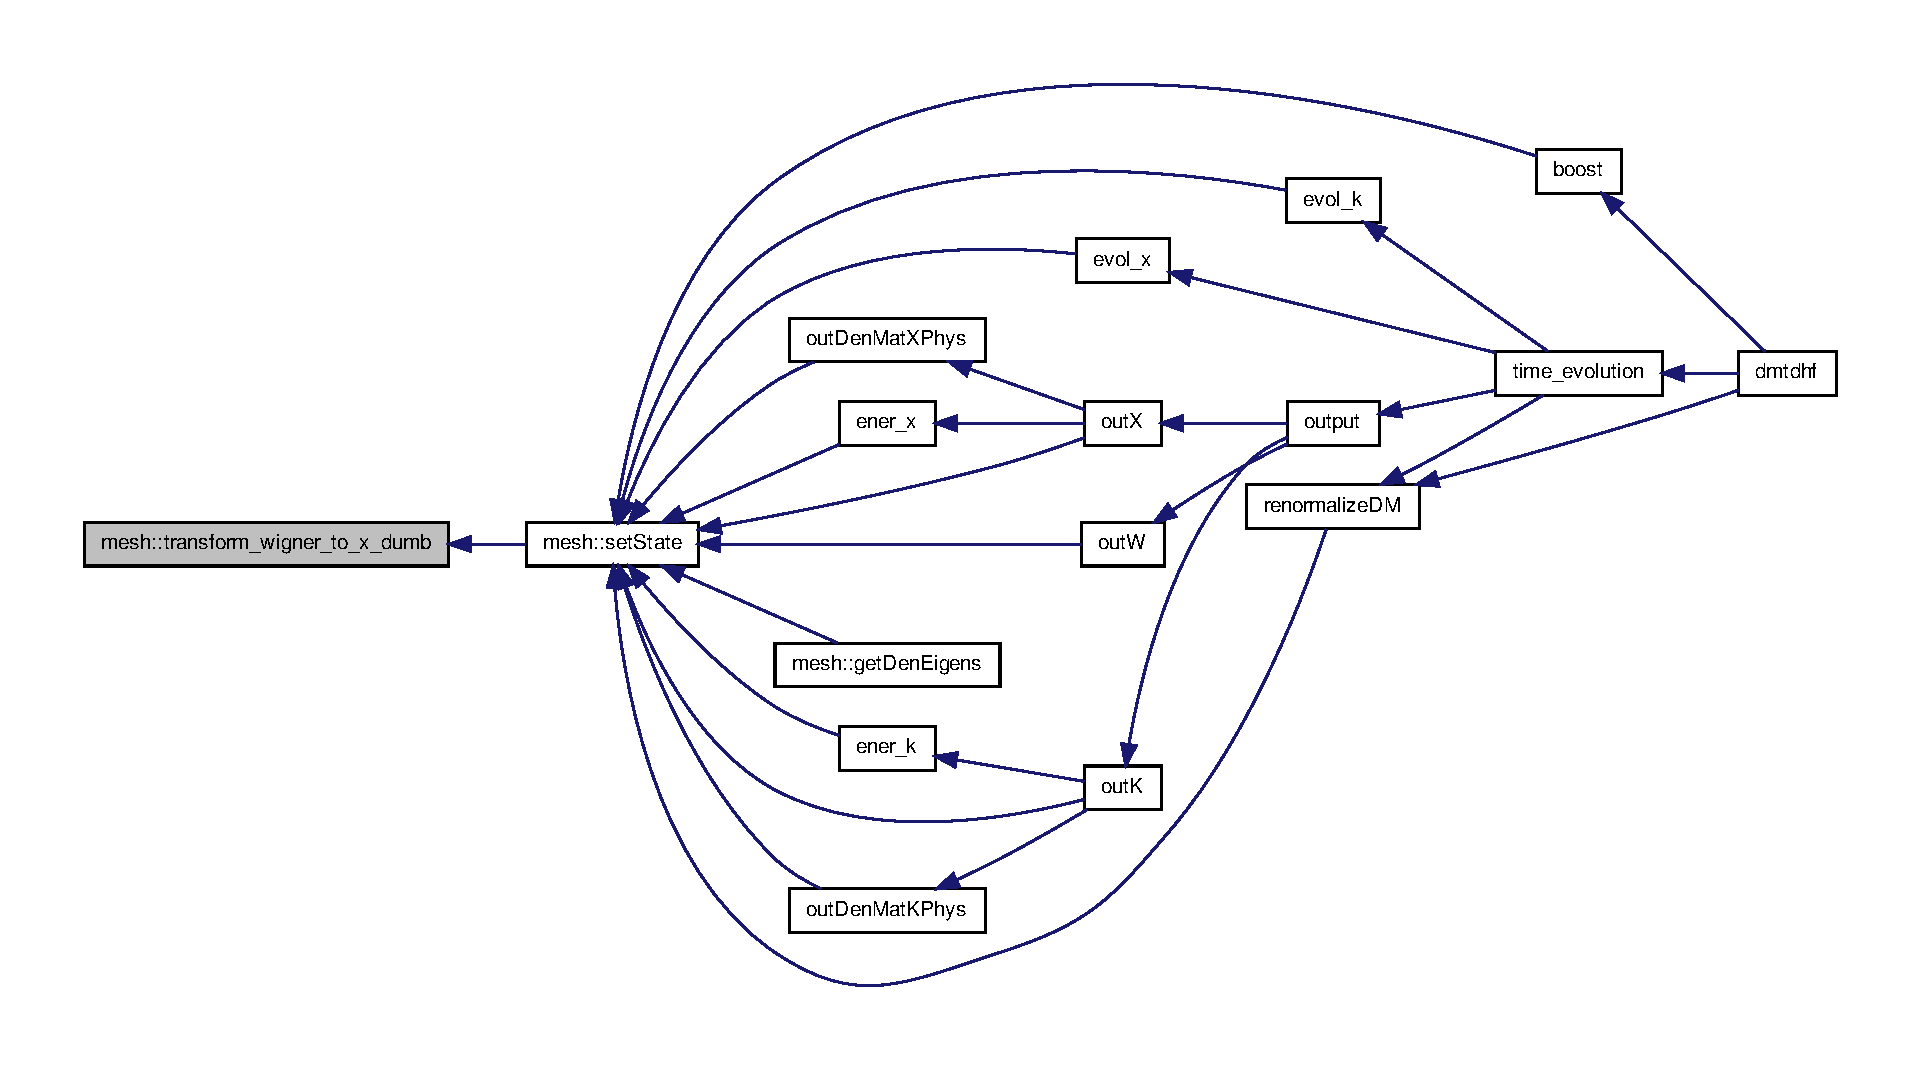
\includegraphics[width=400pt]{namespacemesh_aee41613b43ab6e2f5a715e21c4227f4c_icgraph}
\end{center}
\end{figure}


\hypertarget{namespacemesh_a59d4c181b47238269732a26ba618696e}{
\index{mesh@{mesh}!transform\_\-wigner\_\-to\_\-x\_\-trig@{transform\_\-wigner\_\-to\_\-x\_\-trig}}
\index{transform\_\-wigner\_\-to\_\-x\_\-trig@{transform\_\-wigner\_\-to\_\-x\_\-trig}!mesh@{mesh}}
\subsubsection[{transform\_\-wigner\_\-to\_\-x\_\-trig}]{\setlength{\rightskip}{0pt plus 5cm}subroutine mesh::transform\_\-wigner\_\-to\_\-x\_\-trig (
\begin{DoxyParamCaption}
{}
\end{DoxyParamCaption}
)}}
\label{namespacemesh_a59d4c181b47238269732a26ba618696e}


Definition at line 736 of file mesh.f90.



Here is the call graph for this function:\nopagebreak
\begin{figure}[H]
\begin{center}
\leavevmode
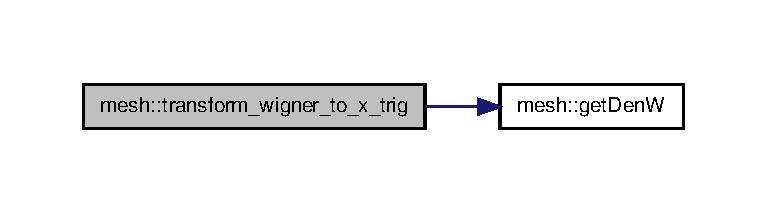
\includegraphics[width=368pt]{namespacemesh_a59d4c181b47238269732a26ba618696e_cgraph}
\end{center}
\end{figure}


\hypertarget{namespacemesh_a4f07e4d7944353c1362be2da4e27b16e}{
\index{mesh@{mesh}!transform\_\-x\_\-to\_\-k\_\-norepeat@{transform\_\-x\_\-to\_\-k\_\-norepeat}}
\index{transform\_\-x\_\-to\_\-k\_\-norepeat@{transform\_\-x\_\-to\_\-k\_\-norepeat}!mesh@{mesh}}
\subsubsection[{transform\_\-x\_\-to\_\-k\_\-norepeat}]{\setlength{\rightskip}{0pt plus 5cm}subroutine mesh::transform\_\-x\_\-to\_\-k\_\-norepeat (
\begin{DoxyParamCaption}
{}
\end{DoxyParamCaption}
)}}
\label{namespacemesh_a4f07e4d7944353c1362be2da4e27b16e}


Definition at line 1042 of file mesh.f90.



Here is the call graph for this function:\nopagebreak
\begin{figure}[H]
\begin{center}
\leavevmode
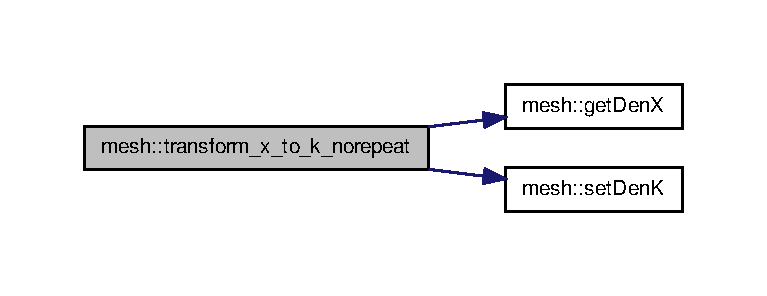
\includegraphics[width=368pt]{namespacemesh_a4f07e4d7944353c1362be2da4e27b16e_cgraph}
\end{center}
\end{figure}


\hypertarget{namespacemesh_aedb02cc0a4ac5c08aef3398b9bca30be}{
\index{mesh@{mesh}!transform\_\-x\_\-to\_\-w\_\-dumb\_\-kshift@{transform\_\-x\_\-to\_\-w\_\-dumb\_\-kshift}}
\index{transform\_\-x\_\-to\_\-w\_\-dumb\_\-kshift@{transform\_\-x\_\-to\_\-w\_\-dumb\_\-kshift}!mesh@{mesh}}
\subsubsection[{transform\_\-x\_\-to\_\-w\_\-dumb\_\-kshift}]{\setlength{\rightskip}{0pt plus 5cm}subroutine mesh::transform\_\-x\_\-to\_\-w\_\-dumb\_\-kshift (
\begin{DoxyParamCaption}
{}
\end{DoxyParamCaption}
)}}
\label{namespacemesh_aedb02cc0a4ac5c08aef3398b9bca30be}


Definition at line 567 of file mesh.f90.



Here is the call graph for this function:\nopagebreak
\begin{figure}[H]
\begin{center}
\leavevmode
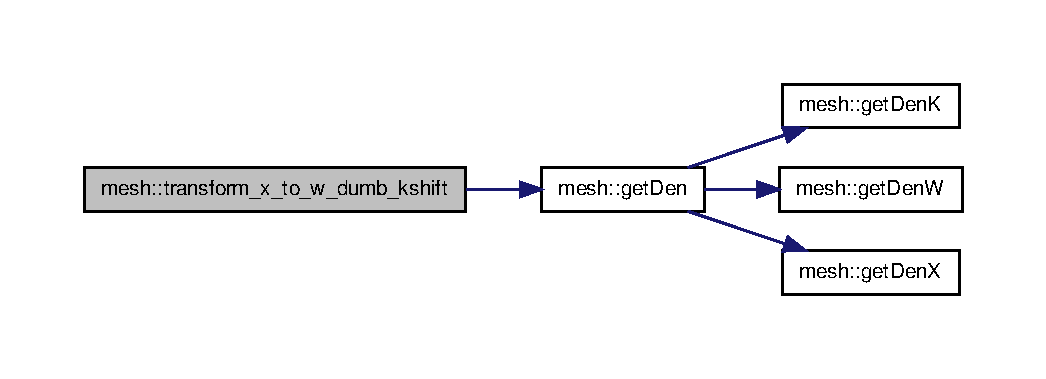
\includegraphics[width=400pt]{namespacemesh_aedb02cc0a4ac5c08aef3398b9bca30be_cgraph}
\end{center}
\end{figure}


\hypertarget{namespacemesh_a1f4e0012bc7646af71d9f56ff2abc54d}{
\index{mesh@{mesh}!transform\_\-x\_\-to\_\-w\_\-norepeat@{transform\_\-x\_\-to\_\-w\_\-norepeat}}
\index{transform\_\-x\_\-to\_\-w\_\-norepeat@{transform\_\-x\_\-to\_\-w\_\-norepeat}!mesh@{mesh}}
\subsubsection[{transform\_\-x\_\-to\_\-w\_\-norepeat}]{\setlength{\rightskip}{0pt plus 5cm}subroutine mesh::transform\_\-x\_\-to\_\-w\_\-norepeat (
\begin{DoxyParamCaption}
{}
\end{DoxyParamCaption}
)}}
\label{namespacemesh_a1f4e0012bc7646af71d9f56ff2abc54d}


Definition at line 1131 of file mesh.f90.

\hypertarget{namespacemesh_adde9e08568da14a3b33bfb7372563330}{
\index{mesh@{mesh}!transform\_\-x\_\-to\_\-w\_\-norepeat\_\-fft@{transform\_\-x\_\-to\_\-w\_\-norepeat\_\-fft}}
\index{transform\_\-x\_\-to\_\-w\_\-norepeat\_\-fft@{transform\_\-x\_\-to\_\-w\_\-norepeat\_\-fft}!mesh@{mesh}}
\subsubsection[{transform\_\-x\_\-to\_\-w\_\-norepeat\_\-fft}]{\setlength{\rightskip}{0pt plus 5cm}subroutine mesh::transform\_\-x\_\-to\_\-w\_\-norepeat\_\-fft (
\begin{DoxyParamCaption}
{}
\end{DoxyParamCaption}
)}}
\label{namespacemesh_adde9e08568da14a3b33bfb7372563330}


Definition at line 1210 of file mesh.f90.



Here is the call graph for this function:\nopagebreak
\begin{figure}[H]
\begin{center}
\leavevmode
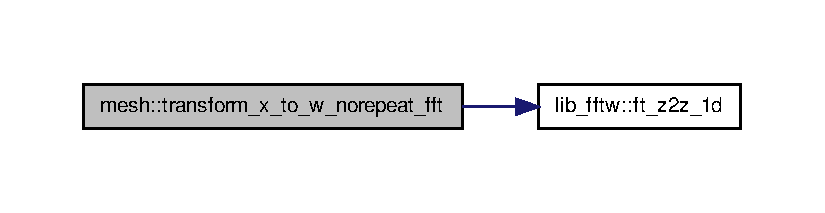
\includegraphics[width=396pt]{namespacemesh_adde9e08568da14a3b33bfb7372563330_cgraph}
\end{center}
\end{figure}


\hypertarget{namespacemesh_ab0c4d2eefb660f80c8bd5a26cfea90bb}{
\index{mesh@{mesh}!transform\_\-x\_\-to\_\-wigner\_\-dumb@{transform\_\-x\_\-to\_\-wigner\_\-dumb}}
\index{transform\_\-x\_\-to\_\-wigner\_\-dumb@{transform\_\-x\_\-to\_\-wigner\_\-dumb}!mesh@{mesh}}
\subsubsection[{transform\_\-x\_\-to\_\-wigner\_\-dumb}]{\setlength{\rightskip}{0pt plus 5cm}subroutine mesh::transform\_\-x\_\-to\_\-wigner\_\-dumb (
\begin{DoxyParamCaption}
{}
\end{DoxyParamCaption}
)}}
\label{namespacemesh_ab0c4d2eefb660f80c8bd5a26cfea90bb}


Definition at line 503 of file mesh.f90.



Here is the call graph for this function:\nopagebreak
\begin{figure}[H]
\begin{center}
\leavevmode
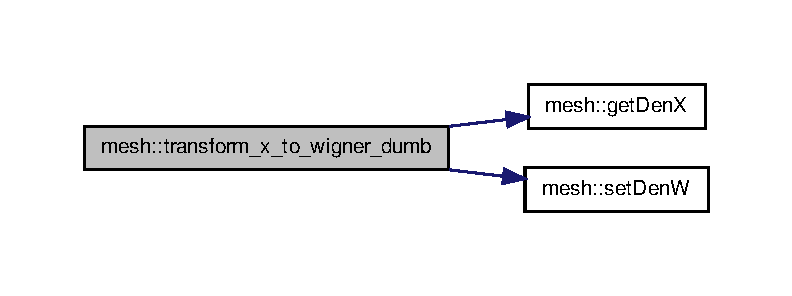
\includegraphics[width=380pt]{namespacemesh_ab0c4d2eefb660f80c8bd5a26cfea90bb_cgraph}
\end{center}
\end{figure}




Here is the caller graph for this function:
\nopagebreak
\begin{figure}[H]
\begin{center}
\leavevmode
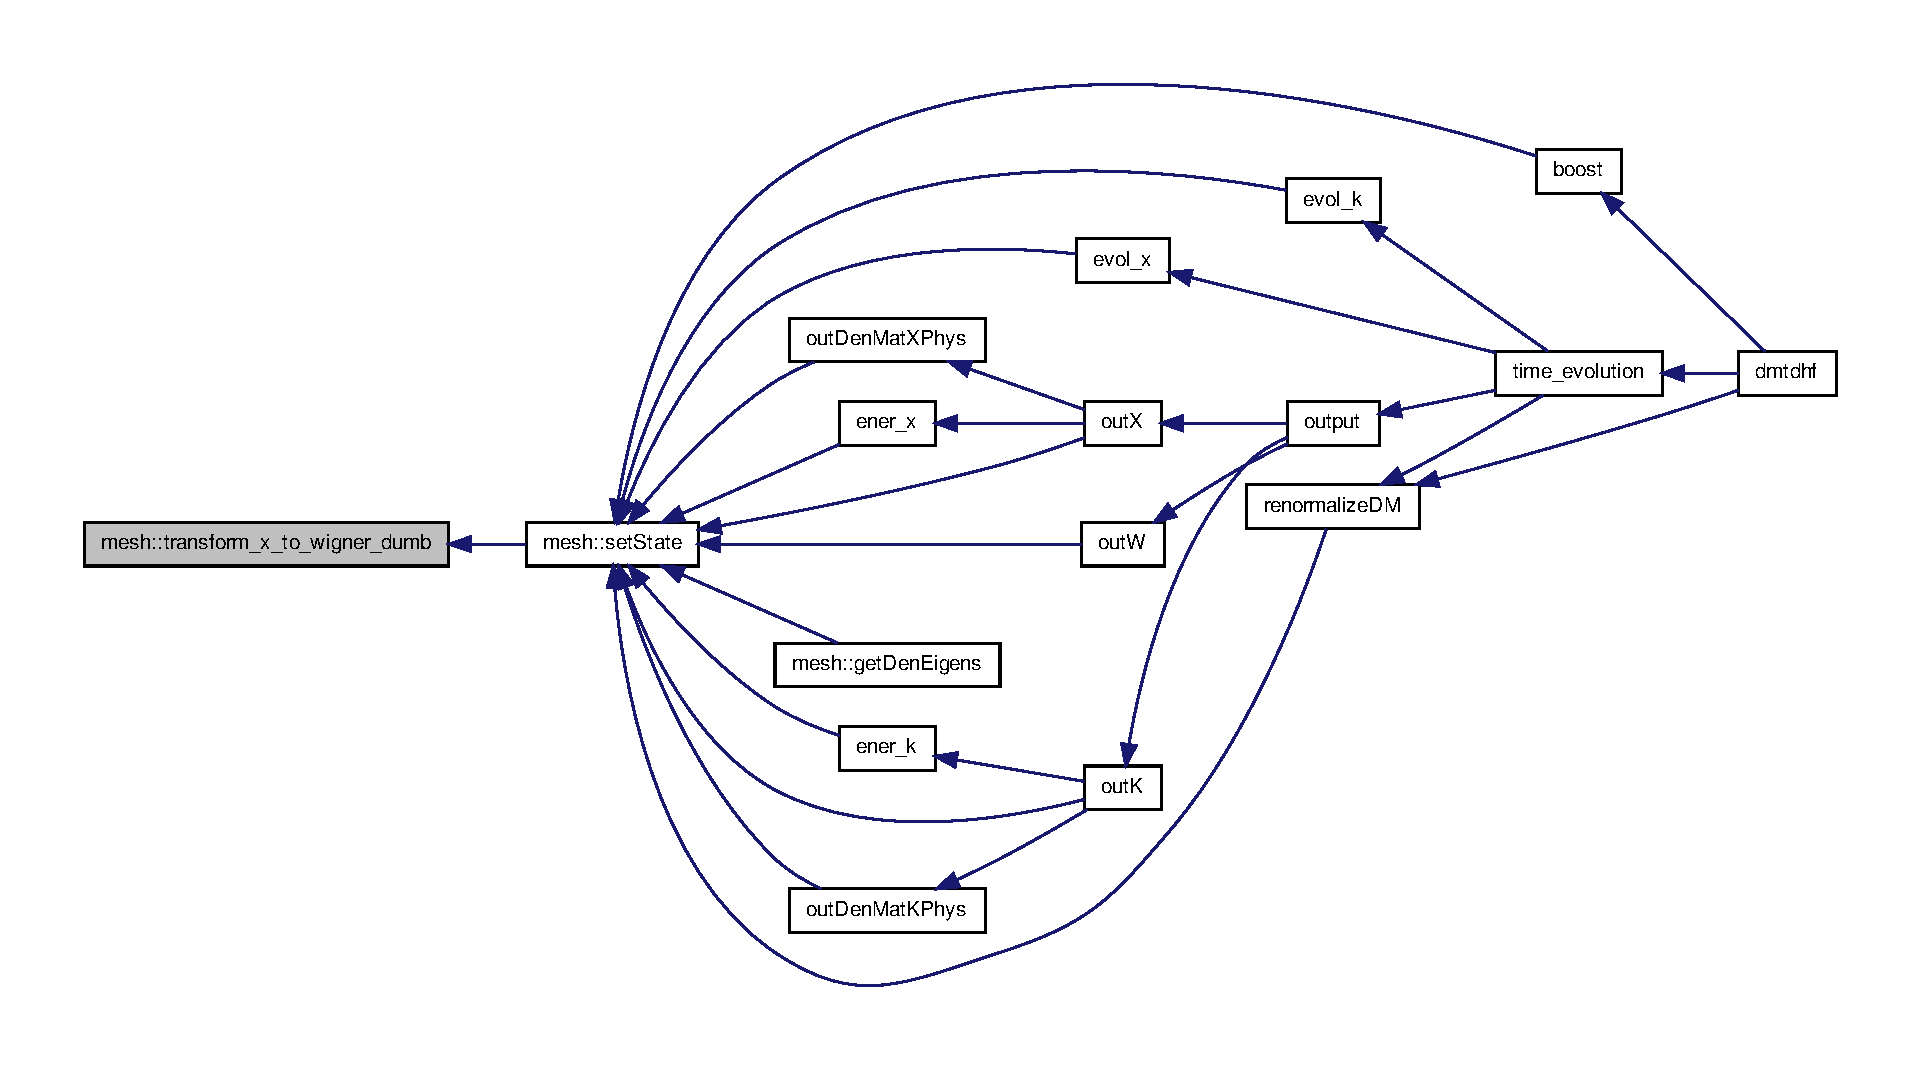
\includegraphics[width=400pt]{namespacemesh_ab0c4d2eefb660f80c8bd5a26cfea90bb_icgraph}
\end{center}
\end{figure}


\hypertarget{namespacemesh_a0469cb1ff672271ea58fa1cca5daec7a}{
\index{mesh@{mesh}!transform\_\-x\_\-to\_\-wigner\_\-trig@{transform\_\-x\_\-to\_\-wigner\_\-trig}}
\index{transform\_\-x\_\-to\_\-wigner\_\-trig@{transform\_\-x\_\-to\_\-wigner\_\-trig}!mesh@{mesh}}
\subsubsection[{transform\_\-x\_\-to\_\-wigner\_\-trig}]{\setlength{\rightskip}{0pt plus 5cm}subroutine mesh::transform\_\-x\_\-to\_\-wigner\_\-trig (
\begin{DoxyParamCaption}
{}
\end{DoxyParamCaption}
)}}
\label{namespacemesh_a0469cb1ff672271ea58fa1cca5daec7a}


Definition at line 453 of file mesh.f90.



Here is the call graph for this function:\nopagebreak
\begin{figure}[H]
\begin{center}
\leavevmode
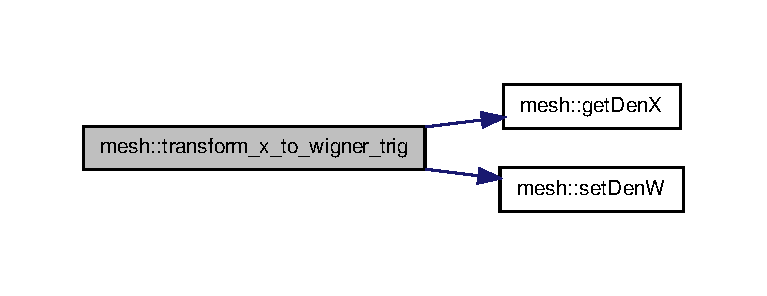
\includegraphics[width=368pt]{namespacemesh_a0469cb1ff672271ea58fa1cca5daec7a_cgraph}
\end{center}
\end{figure}




\subsection{Variable Documentation}
\hypertarget{namespacemesh_a93c5cfe69a9cda5c977adaf99030481d}{
\index{mesh@{mesh}!delka@{delka}}
\index{delka@{delka}!mesh@{mesh}}
\subsubsection[{delka}]{\setlength{\rightskip}{0pt plus 5cm}REAL$\ast$8 {\bf mesh::delka}}}
\label{namespacemesh_a93c5cfe69a9cda5c977adaf99030481d}


Definition at line 50 of file mesh.f90.

\hypertarget{namespacemesh_a30ce8cdfbc09510b555134e5ee1c2472}{
\index{mesh@{mesh}!delkr@{delkr}}
\index{delkr@{delkr}!mesh@{mesh}}
\subsubsection[{delkr}]{\setlength{\rightskip}{0pt plus 5cm}REAL$\ast$8 {\bf mesh::delkr}}}
\label{namespacemesh_a30ce8cdfbc09510b555134e5ee1c2472}


Definition at line 51 of file mesh.f90.

\hypertarget{namespacemesh_a4bbd964b605a9fedc6fd4b5feaf2d226}{
\index{mesh@{mesh}!delxa@{delxa}}
\index{delxa@{delxa}!mesh@{mesh}}
\subsubsection[{delxa}]{\setlength{\rightskip}{0pt plus 5cm}REAL$\ast$8 {\bf mesh::delxa}}}
\label{namespacemesh_a4bbd964b605a9fedc6fd4b5feaf2d226}


Definition at line 48 of file mesh.f90.

\hypertarget{namespacemesh_a8517784a828d82832ad38e911e58cdf1}{
\index{mesh@{mesh}!delxr@{delxr}}
\index{delxr@{delxr}!mesh@{mesh}}
\subsubsection[{delxr}]{\setlength{\rightskip}{0pt plus 5cm}REAL$\ast$8 {\bf mesh::delxr}}}
\label{namespacemesh_a8517784a828d82832ad38e911e58cdf1}


Definition at line 49 of file mesh.f90.

\hypertarget{namespacemesh_a88e07a02f831434825843fa4d74b7bc0}{
\index{mesh@{mesh}!den\_\-im@{den\_\-im}}
\index{den\_\-im@{den\_\-im}!mesh@{mesh}}
\subsubsection[{den\_\-im}]{\setlength{\rightskip}{0pt plus 5cm}REAL$\ast$8,dimension(:,:),allocatable {\bf mesh::den\_\-im}}}
\label{namespacemesh_a88e07a02f831434825843fa4d74b7bc0}


Definition at line 60 of file mesh.f90.

\hypertarget{namespacemesh_af15f870e8317605924334a07ecfe3b28}{
\index{mesh@{mesh}!den\_\-re@{den\_\-re}}
\index{den\_\-re@{den\_\-re}!mesh@{mesh}}
\subsubsection[{den\_\-re}]{\setlength{\rightskip}{0pt plus 5cm}REAL$\ast$8,dimension(:,:),allocatable {\bf mesh::den\_\-re}}}
\label{namespacemesh_af15f870e8317605924334a07ecfe3b28}


Definition at line 60 of file mesh.f90.

\hypertarget{namespacemesh_ad78af6f9bdcc56004176e07e81d419f8}{
\index{mesh@{mesh}!denmat@{denmat}}
\index{denmat@{denmat}!mesh@{mesh}}
\subsubsection[{denmat}]{\setlength{\rightskip}{0pt plus 5cm}complex$\ast$16,dimension(:,:),allocatable {\bf mesh::denmat}}}
\label{namespacemesh_ad78af6f9bdcc56004176e07e81d419f8}


Definition at line 61 of file mesh.f90.

\hypertarget{namespacemesh_ac1de4684ee911518c05caaa4c6dcf484}{
\index{mesh@{mesh}!denmat2@{denmat2}}
\index{denmat2@{denmat2}!mesh@{mesh}}
\subsubsection[{denmat2}]{\setlength{\rightskip}{0pt plus 5cm}complex$\ast$16,dimension(:,:),allocatable {\bf mesh::denmat2}}}
\label{namespacemesh_ac1de4684ee911518c05caaa4c6dcf484}


Definition at line 62 of file mesh.f90.

\hypertarget{namespacemesh_a451ed2546542175ea54b5c9a780b5462}{
\index{mesh@{mesh}!denState@{denState}}
\index{denState@{denState}!mesh@{mesh}}
\subsubsection[{denState}]{\setlength{\rightskip}{0pt plus 5cm}integer {\bf mesh::denState}}}
\label{namespacemesh_a451ed2546542175ea54b5c9a780b5462}


Definition at line 63 of file mesh.f90.

\hypertarget{namespacemesh_a43130e9d2b4c80b7862ea7d6226a7a4d}{
\index{mesh@{mesh}!facd@{facd}}
\index{facd@{facd}!mesh@{mesh}}
\subsubsection[{facd}]{\setlength{\rightskip}{0pt plus 5cm}REAL$\ast$8 {\bf mesh::facd}}}
\label{namespacemesh_a43130e9d2b4c80b7862ea7d6226a7a4d}


Definition at line 56 of file mesh.f90.

\hypertarget{namespacemesh_a6103232aa20c5d4619b9016bda1e0cbe}{
\index{mesh@{mesh}!iNka2@{iNka2}}
\index{iNka2@{iNka2}!mesh@{mesh}}
\subsubsection[{iNka2}]{\setlength{\rightskip}{0pt plus 5cm}INTEGER,allocatable {\bf mesh::iNka2}}}
\label{namespacemesh_a6103232aa20c5d4619b9016bda1e0cbe}


Definition at line 72 of file mesh.f90.

\hypertarget{namespacemesh_a4a147979d603b0d2f61b08be8bd3e40e}{
\index{mesh@{mesh}!iNkr2@{iNkr2}}
\index{iNkr2@{iNkr2}!mesh@{mesh}}
\subsubsection[{iNkr2}]{\setlength{\rightskip}{0pt plus 5cm}INTEGER,allocatable {\bf mesh::iNkr2}}}
\label{namespacemesh_a4a147979d603b0d2f61b08be8bd3e40e}


Definition at line 72 of file mesh.f90.

\hypertarget{namespacemesh_ac40d4b15a769844035c498c2ed396e4c}{
\index{mesh@{mesh}!isReflectedLR@{isReflectedLR}}
\index{isReflectedLR@{isReflectedLR}!mesh@{mesh}}
\subsubsection[{isReflectedLR}]{\setlength{\rightskip}{0pt plus 5cm}logical {\bf mesh::isReflectedLR}}}
\label{namespacemesh_ac40d4b15a769844035c498c2ed396e4c}


Definition at line 69 of file mesh.f90.

\hypertarget{namespacemesh_acdc9121ee94e3c62c59255106d13fddd}{
\index{mesh@{mesh}!ka@{ka}}
\index{ka@{ka}!mesh@{mesh}}
\subsubsection[{ka}]{\setlength{\rightskip}{0pt plus 5cm}REAL$\ast$8,dimension(:),allocatable {\bf mesh::ka}}}
\label{namespacemesh_acdc9121ee94e3c62c59255106d13fddd}


Definition at line 57 of file mesh.f90.

\hypertarget{namespacemesh_a9b60e77e26ab439594233774c928b35c}{
\index{mesh@{mesh}!kLa@{kLa}}
\index{kLa@{kLa}!mesh@{mesh}}
\subsubsection[{kLa}]{\setlength{\rightskip}{0pt plus 5cm}real$\ast$8 {\bf mesh::kLa}}}
\label{namespacemesh_a9b60e77e26ab439594233774c928b35c}


Definition at line 29 of file mesh.f90.

\hypertarget{namespacemesh_a0eb10f03f0d716aafcb803855dff1b80}{
\index{mesh@{mesh}!kr@{kr}}
\index{kr@{kr}!mesh@{mesh}}
\subsubsection[{kr}]{\setlength{\rightskip}{0pt plus 5cm}REAL$\ast$8,dimension(:),allocatable {\bf mesh::kr}}}
\label{namespacemesh_a0eb10f03f0d716aafcb803855dff1b80}


Definition at line 57 of file mesh.f90.

\hypertarget{namespacemesh_aa7d7e6a7c12152ba29110facf1d664ce}{
\index{mesh@{mesh}!maxxim@{maxxim}}
\index{maxxim@{maxxim}!mesh@{mesh}}
\subsubsection[{maxxim}]{\setlength{\rightskip}{0pt plus 5cm}real$\ast$8 {\bf mesh::maxxim}}}
\label{namespacemesh_aa7d7e6a7c12152ba29110facf1d664ce}


Definition at line 76 of file mesh.f90.

\hypertarget{namespacemesh_a58029be857a15564e9ebaee23b4d887a}{
\index{mesh@{mesh}!MOMENTUM@{MOMENTUM}}
\index{MOMENTUM@{MOMENTUM}!mesh@{mesh}}
\subsubsection[{MOMENTUM}]{\setlength{\rightskip}{0pt plus 5cm}integer,parameter {\bf mesh::MOMENTUM} = 2}}
\label{namespacemesh_a58029be857a15564e9ebaee23b4d887a}


Definition at line 67 of file mesh.f90.

\hypertarget{namespacemesh_ab0bd6c4de110f0158d8a3aedd0be3907}{
\index{mesh@{mesh}!Nka@{Nka}}
\index{Nka@{Nka}!mesh@{mesh}}
\subsubsection[{Nka}]{\setlength{\rightskip}{0pt plus 5cm}INTEGER {\bf mesh::Nka}}}
\label{namespacemesh_ab0bd6c4de110f0158d8a3aedd0be3907}


Definition at line 34 of file mesh.f90.

\hypertarget{namespacemesh_abad69d3716a915fa710b7ba198f90f1b}{
\index{mesh@{mesh}!Nka2@{Nka2}}
\index{Nka2@{Nka2}!mesh@{mesh}}
\subsubsection[{Nka2}]{\setlength{\rightskip}{0pt plus 5cm}INTEGER {\bf mesh::Nka2}}}
\label{namespacemesh_abad69d3716a915fa710b7ba198f90f1b}


Definition at line 37 of file mesh.f90.

\hypertarget{namespacemesh_a910970a3de4d93dbe22c5990a246c360}{
\index{mesh@{mesh}!Nkam@{Nkam}}
\index{Nkam@{Nkam}!mesh@{mesh}}
\subsubsection[{Nkam}]{\setlength{\rightskip}{0pt plus 5cm}integer {\bf mesh::Nkam}}}
\label{namespacemesh_a910970a3de4d93dbe22c5990a246c360}


Definition at line 43 of file mesh.f90.

\hypertarget{namespacemesh_a29b4b004a2f1961e2ad6ea8faf2bc447}{
\index{mesh@{mesh}!Nkax@{Nkax}}
\index{Nkax@{Nkax}!mesh@{mesh}}
\subsubsection[{Nkax}]{\setlength{\rightskip}{0pt plus 5cm}integer {\bf mesh::Nkax}}}
\label{namespacemesh_a29b4b004a2f1961e2ad6ea8faf2bc447}


Definition at line 44 of file mesh.f90.

\hypertarget{namespacemesh_a1d27552200f5f3bf302bcbd55bb2ccf5}{
\index{mesh@{mesh}!Nkr@{Nkr}}
\index{Nkr@{Nkr}!mesh@{mesh}}
\subsubsection[{Nkr}]{\setlength{\rightskip}{0pt plus 5cm}integer {\bf mesh::Nkr}}}
\label{namespacemesh_a1d27552200f5f3bf302bcbd55bb2ccf5}


Definition at line 35 of file mesh.f90.

\hypertarget{namespacemesh_a55a4e9bc46503b5f1fddde6e621a0b86}{
\index{mesh@{mesh}!Nkr2@{Nkr2}}
\index{Nkr2@{Nkr2}!mesh@{mesh}}
\subsubsection[{Nkr2}]{\setlength{\rightskip}{0pt plus 5cm}INTEGER {\bf mesh::Nkr2}}}
\label{namespacemesh_a55a4e9bc46503b5f1fddde6e621a0b86}


Definition at line 36 of file mesh.f90.

\hypertarget{namespacemesh_ac39a727e6167a944fb3c7997bfd11de4}{
\index{mesh@{mesh}!Nkrm@{Nkrm}}
\index{Nkrm@{Nkrm}!mesh@{mesh}}
\subsubsection[{Nkrm}]{\setlength{\rightskip}{0pt plus 5cm}integer {\bf mesh::Nkrm}}}
\label{namespacemesh_ac39a727e6167a944fb3c7997bfd11de4}


Definition at line 45 of file mesh.f90.

\hypertarget{namespacemesh_a1750b1e7febac49c12606a9cbf2c4ac2}{
\index{mesh@{mesh}!Nkrx@{Nkrx}}
\index{Nkrx@{Nkrx}!mesh@{mesh}}
\subsubsection[{Nkrx}]{\setlength{\rightskip}{0pt plus 5cm}integer {\bf mesh::Nkrx}}}
\label{namespacemesh_a1750b1e7febac49c12606a9cbf2c4ac2}


Definition at line 46 of file mesh.f90.

\hypertarget{namespacemesh_a753aba092294fa8bffbee1fc1b099584}{
\index{mesh@{mesh}!norm\_\-thy@{norm\_\-thy}}
\index{norm\_\-thy@{norm\_\-thy}!mesh@{mesh}}
\subsubsection[{norm\_\-thy}]{\setlength{\rightskip}{0pt plus 5cm}real (Long) {\bf mesh::norm\_\-thy}}}
\label{namespacemesh_a753aba092294fa8bffbee1fc1b099584}


Definition at line 53 of file mesh.f90.

\hypertarget{namespacemesh_ae1fae2c81e5dc8a2e00f92d4ccb24444}{
\index{mesh@{mesh}!Nxa@{Nxa}}
\index{Nxa@{Nxa}!mesh@{mesh}}
\subsubsection[{Nxa}]{\setlength{\rightskip}{0pt plus 5cm}INTEGER {\bf mesh::Nxa}}}
\label{namespacemesh_ae1fae2c81e5dc8a2e00f92d4ccb24444}


Definition at line 30 of file mesh.f90.

\hypertarget{namespacemesh_a632597390bacfaae4c10d8cb907b2aec}{
\index{mesh@{mesh}!Nxa2@{Nxa2}}
\index{Nxa2@{Nxa2}!mesh@{mesh}}
\subsubsection[{Nxa2}]{\setlength{\rightskip}{0pt plus 5cm}INTEGER {\bf mesh::Nxa2}}}
\label{namespacemesh_a632597390bacfaae4c10d8cb907b2aec}


Definition at line 32 of file mesh.f90.

\hypertarget{namespacemesh_abe9e186636ba22271b7b4550522dceaf}{
\index{mesh@{mesh}!Nxam@{Nxam}}
\index{Nxam@{Nxam}!mesh@{mesh}}
\subsubsection[{Nxam}]{\setlength{\rightskip}{0pt plus 5cm}integer {\bf mesh::Nxam}}}
\label{namespacemesh_abe9e186636ba22271b7b4550522dceaf}


Definition at line 39 of file mesh.f90.

\hypertarget{namespacemesh_a258a6753e659f5aad4d77626f82c674c}{
\index{mesh@{mesh}!Nxax@{Nxax}}
\index{Nxax@{Nxax}!mesh@{mesh}}
\subsubsection[{Nxax}]{\setlength{\rightskip}{0pt plus 5cm}integer {\bf mesh::Nxax}}}
\label{namespacemesh_a258a6753e659f5aad4d77626f82c674c}


Definition at line 40 of file mesh.f90.

\hypertarget{namespacemesh_a4fae0f9e86bfdcb8fec5dc0aefd8fe71}{
\index{mesh@{mesh}!Nxr@{Nxr}}
\index{Nxr@{Nxr}!mesh@{mesh}}
\subsubsection[{Nxr}]{\setlength{\rightskip}{0pt plus 5cm}INTEGER {\bf mesh::Nxr}}}
\label{namespacemesh_a4fae0f9e86bfdcb8fec5dc0aefd8fe71}


Definition at line 31 of file mesh.f90.

\hypertarget{namespacemesh_a7838433bd66eb8c9d5155928904d9a5a}{
\index{mesh@{mesh}!Nxr2@{Nxr2}}
\index{Nxr2@{Nxr2}!mesh@{mesh}}
\subsubsection[{Nxr2}]{\setlength{\rightskip}{0pt plus 5cm}INTEGER {\bf mesh::Nxr2}}}
\label{namespacemesh_a7838433bd66eb8c9d5155928904d9a5a}


Definition at line 33 of file mesh.f90.

\hypertarget{namespacemesh_a3dc98a3a965cb38fc45c4b7801f0f3d2}{
\index{mesh@{mesh}!Nxrm@{Nxrm}}
\index{Nxrm@{Nxrm}!mesh@{mesh}}
\subsubsection[{Nxrm}]{\setlength{\rightskip}{0pt plus 5cm}integer {\bf mesh::Nxrm}}}
\label{namespacemesh_a3dc98a3a965cb38fc45c4b7801f0f3d2}


Definition at line 41 of file mesh.f90.

\hypertarget{namespacemesh_a3836bb9dd0f99e784aecf5ffac36418a}{
\index{mesh@{mesh}!Nxrx@{Nxrx}}
\index{Nxrx@{Nxrx}!mesh@{mesh}}
\subsubsection[{Nxrx}]{\setlength{\rightskip}{0pt plus 5cm}integer {\bf mesh::Nxrx}}}
\label{namespacemesh_a3836bb9dd0f99e784aecf5ffac36418a}


Definition at line 42 of file mesh.f90.

\hypertarget{namespacemesh_a6e7109b1ed1096ce6c3dbacaa4920158}{
\index{mesh@{mesh}!potDiag@{potDiag}}
\index{potDiag@{potDiag}!mesh@{mesh}}
\subsubsection[{potDiag}]{\setlength{\rightskip}{0pt plus 5cm}real$\ast$8,allocatable {\bf mesh::potDiag}}}
\label{namespacemesh_a6e7109b1ed1096ce6c3dbacaa4920158}


Definition at line 74 of file mesh.f90.

\hypertarget{namespacemesh_a0c6bae5d6531a6b0f0428c0c056f759d}{
\index{mesh@{mesh}!SPACE@{SPACE}}
\index{SPACE@{SPACE}!mesh@{mesh}}
\subsubsection[{SPACE}]{\setlength{\rightskip}{0pt plus 5cm}integer,parameter {\bf mesh::SPACE} = 0}}
\label{namespacemesh_a0c6bae5d6531a6b0f0428c0c056f759d}


Definition at line 65 of file mesh.f90.

\hypertarget{namespacemesh_a4e989d120872f8573cf4454bfc6a0d31}{
\index{mesh@{mesh}!WIGNER@{WIGNER}}
\index{WIGNER@{WIGNER}!mesh@{mesh}}
\subsubsection[{WIGNER}]{\setlength{\rightskip}{0pt plus 5cm}integer,parameter {\bf mesh::WIGNER} = 1}}
\label{namespacemesh_a4e989d120872f8573cf4454bfc6a0d31}


Definition at line 66 of file mesh.f90.

\hypertarget{namespacemesh_af9469b274e48a8fcc34f1c8df7976271}{
\index{mesh@{mesh}!xa@{xa}}
\index{xa@{xa}!mesh@{mesh}}
\subsubsection[{xa}]{\setlength{\rightskip}{0pt plus 5cm}REAL$\ast$8,dimension(:),allocatable {\bf mesh::xa}}}
\label{namespacemesh_af9469b274e48a8fcc34f1c8df7976271}


Definition at line 57 of file mesh.f90.

\hypertarget{namespacemesh_a7b0412308700e4488efc480ace9412b8}{
\index{mesh@{mesh}!xLa@{xLa}}
\index{xLa@{xLa}!mesh@{mesh}}
\subsubsection[{xLa}]{\setlength{\rightskip}{0pt plus 5cm}REAL$\ast$8 {\bf mesh::xLa}}}
\label{namespacemesh_a7b0412308700e4488efc480ace9412b8}


Definition at line 27 of file mesh.f90.

\hypertarget{namespacemesh_a4ad69b5cc7ea5c0bd0f1f8d39fc3f604}{
\index{mesh@{mesh}!xLr@{xLr}}
\index{xLr@{xLr}!mesh@{mesh}}
\subsubsection[{xLr}]{\setlength{\rightskip}{0pt plus 5cm}REAL$\ast$8 {\bf mesh::xLr}}}
\label{namespacemesh_a4ad69b5cc7ea5c0bd0f1f8d39fc3f604}


Definition at line 28 of file mesh.f90.

\hypertarget{namespacemesh_a0351493d48c86a4a92f34aa94f8cc099}{
\index{mesh@{mesh}!xr@{xr}}
\index{xr@{xr}!mesh@{mesh}}
\subsubsection[{xr}]{\setlength{\rightskip}{0pt plus 5cm}REAL$\ast$8,dimension(:),allocatable {\bf mesh::xr}}}
\label{namespacemesh_a0351493d48c86a4a92f34aa94f8cc099}


Definition at line 57 of file mesh.f90.


\hypertarget{namespacephys__cons}{
\section{phys\_\-cons Module Reference}
\label{namespacephys__cons}\index{phys\_\-cons@{phys\_\-cons}}
}


Stores mathematical and physical constants, both in SI units and user-\/defined units.  


\subsection*{Functions/Subroutines}
\begin{DoxyCompactItemize}
\item 
subroutine \hyperlink{namespacephys__cons_a2197fe7eff35572113dcf41a6493794c}{phys\_\-cons\_\-initialize} ()
\begin{DoxyCompactList}\small\item\em Initializes module, assumes current system of units is SI. \item\end{DoxyCompactList}\item 
subroutine \hyperlink{namespacephys__cons_abfc9a7567c3e76fdbbad91b88b46426e}{phys\_\-cons\_\-initialize\_\-SI}
\item 
subroutine \hyperlink{namespacephys__cons_ab13f84d8b6f574eb73870a2964a82b8b}{phys\_\-cons\_\-initializeNuclear}
\begin{DoxyCompactList}\small\item\em Initializes physical constants, using nuclear system: \item\end{DoxyCompactList}\end{DoxyCompactItemize}
\subsection*{Variables}
\begin{DoxyCompactItemize}
\item 
complex $\ast$16, parameter \hyperlink{namespacephys__cons_af15f96806bfb6b9c6b1a279971d5d34b}{imagi} = cmplx(0.d0, 1.d0, 8)
\item 
REAL(long), parameter \hyperlink{namespacephys__cons_aae3c6cb8ae765b0262bb110ff739ba9d}{pi} = 4d0$\ast$atan(1d0)
\item 
real(long), parameter \hyperlink{namespacephys__cons_aa8683f00f4216acc1822dfcb85b1ee00}{invpi} = 1d0/pi
\item 
real(long), parameter \hyperlink{namespacephys__cons_a369d33713444a99a71f80a74c0652d4e}{invsqrt2pi} = 1d0/sqrt(2d0$\ast$pi)
\item 
real(Long), parameter \hyperlink{namespacephys__cons_ae265fad966cfc841f9a073a52955d742}{SI\_\-SPEED\_\-OF\_\-LIGHT} = 299792458d0
\begin{DoxyCompactList}\small\item\em speed of light in vacuum, c, in m s$^{\mbox{-\/1}}$ , from 2010 CODATA recommended values \item\end{DoxyCompactList}\item 
real(Long), parameter \hyperlink{namespacephys__cons_a5547546b06eb8853e52e304b25cc7596}{SI\_\-SPEED\_\-OF\_\-LIGHT\_\-D} = 0d0
\begin{DoxyCompactList}\small\item\em uncertainty \item\end{DoxyCompactList}\item 
real(Long) \hyperlink{namespacephys__cons_ac31faa4bb5e82aecbdffa3b3d43a1736}{SPEED\_\-OF\_\-LIGHT}
\begin{DoxyCompactList}\small\item\em in current units \item\end{DoxyCompactList}\item 
real(Long), parameter \hyperlink{namespacephys__cons_ab49e79c21c913c5857dedf2c555d2c21}{SI\_\-PLANCKS\_\-CONSTANT\_\-HBAR} = 1.054571726e-\/34\_\-Long
\begin{DoxyCompactList}\small\item\em Planck's constant divided by 2π, ℏ, in J s, from 2010 CODATA. \item\end{DoxyCompactList}\item 
real(Long), parameter \hyperlink{namespacephys__cons_af8ab82739d58ac3a1e1d9c97d3cfb4da}{SI\_\-PLANCKS\_\-CONSTANT\_\-HBAR\_\-D} = 0.000000047e-\/34\_\-Long
\begin{DoxyCompactList}\small\item\em uncertainty \item\end{DoxyCompactList}\item 
real(Long) \hyperlink{namespacephys__cons_af0b754235993060b14fc81b7d1f702a5}{PLANCKS\_\-CONSTANT\_\-HBAR}
\begin{DoxyCompactList}\small\item\em in current units \item\end{DoxyCompactList}\item 
real(Long), parameter \hyperlink{namespacephys__cons_ab117ad83bb79e4ed199d17f3c63ec4b3}{SI\_\-MASS\_\-NEUTRON} = 1.674927351e-\/27\_\-Long
\begin{DoxyCompactList}\small\item\em mass of the neutron, m$_{\mbox{n}}$ , in kg, from 2010 CODATA \item\end{DoxyCompactList}\item 
real(Long), parameter \hyperlink{namespacephys__cons_af635c94d544c5bc6dcb05186a9f81d84}{SI\_\-MASS\_\-NEUTRON\_\-D} = 0.000000074e-\/27\_\-Long
\begin{DoxyCompactList}\small\item\em uncertainty \item\end{DoxyCompactList}\item 
real(Long) \hyperlink{namespacephys__cons_abeff422917cc48601644e90ab12fb7c0}{MASS\_\-NEUTRON}
\begin{DoxyCompactList}\small\item\em in current units \item\end{DoxyCompactList}\item 
real(Long), parameter \hyperlink{namespacephys__cons_a6a740864089f117512dc89ea53f3dc5f}{SI\_\-MASS\_\-PROTON} = 1.672621777e-\/27\_\-Long
\begin{DoxyCompactList}\small\item\em mass of the proton, m$_{\mbox{p}}$ , in kg. \item\end{DoxyCompactList}\item 
real(Long), parameter \hyperlink{namespacephys__cons_a3c37a18a918519962cfc26597082d53d}{SI\_\-MASS\_\-PROTON\_\-D} = 0.000000074e-\/27\_\-Long
\begin{DoxyCompactList}\small\item\em uncertainty \item\end{DoxyCompactList}\item 
real(Long) \hyperlink{namespacephys__cons_a20e8ed3d7ff389588ce024048c5ccf85}{MASS\_\-PROTON}
\begin{DoxyCompactList}\small\item\em in current units \item\end{DoxyCompactList}\item 
REAL(long), parameter \hyperlink{namespacephys__cons_a4b10513970a98ad78b85723c60d9a8b6}{rho0} = 0.16d0
\item 
REAL(long), parameter \hyperlink{namespacephys__cons_a2d3539e3579b581a4e69eff7347b4fa2}{hbc} = 197.326963d0
\item 
REAL(long), parameter \hyperlink{namespacephys__cons_a030a10874bc73b7d042adb32fad75614}{hbc2} = \hyperlink{namespacephys__cons_a2d3539e3579b581a4e69eff7347b4fa2}{hbc}$\ast$\hyperlink{namespacephys__cons_a2d3539e3579b581a4e69eff7347b4fa2}{hbc}
\item 
REAL(long), parameter \hyperlink{namespacephys__cons_ae2a4cb4e421fe399f19d0729b5617fed}{mp} = 938.272013d0
\item 
REAL(long), parameter \hyperlink{namespacephys__cons_ad68aaba74b75e1e13f1367c1eb0904c1}{mn} = 939.565560d0
\item 
REAL(long), parameter \hyperlink{namespacephys__cons_afa35c20a6e2a70b58142d10071eeef10}{m0} = (\hyperlink{namespacephys__cons_ae2a4cb4e421fe399f19d0729b5617fed}{mp}+\hyperlink{namespacephys__cons_ad68aaba74b75e1e13f1367c1eb0904c1}{mn})$\ast$0.5d0
\begin{DoxyCompactList}\small\item\em mass of particle being evolved in time \item\end{DoxyCompactList}\item 
REAL(Long), parameter \hyperlink{namespacephys__cons_a02e8bb2c808e0085a317bf36ff79ae2a}{a0} = 931.494028d0
\item 
REAL(long), parameter \hyperlink{namespacephys__cons_ad97ad749ef4f8f66c56a0facb7394cb5}{hm} = \hyperlink{namespacephys__cons_a2d3539e3579b581a4e69eff7347b4fa2}{hbc}$\ast$\hyperlink{namespacephys__cons_a2d3539e3579b581a4e69eff7347b4fa2}{hbc}/(2.d0$\ast$\hyperlink{namespacephys__cons_afa35c20a6e2a70b58142d10071eeef10}{m0})
\item 
REAL(long), parameter \hyperlink{namespacephys__cons_a553e3e17652770308e6bffcb8fcb5a95}{deg} = 4.d0
\item 
real(Long), parameter \hyperlink{namespacephys__cons_a9e80f5448f5f42cf9983890809e55d88}{MASS\_\-NEUTRON\_\-MEV\_\-C2} = 939.565379\_\-Long
\begin{DoxyCompactList}\small\item\em Mass of the neutron, in MeV/c$^{\mbox{$^\wedge$2}}$ , from 2010 CODATA. \item\end{DoxyCompactList}\item 
real(Long), parameter \hyperlink{namespacephys__cons_ab5fb46dc243eb307a344a134a593edd0}{MASS\_\-NEUTRON\_\-MEV\_\-C2\_\-D} = 0.000021\_\-Long
\begin{DoxyCompactList}\small\item\em uncertainty \item\end{DoxyCompactList}\item 
real(Long), parameter \hyperlink{namespacephys__cons_a3460d18828c87b266ab35b1cdeb4a0a5}{MASS\_\-PROTON\_\-MEV\_\-C2} = 938.272046\_\-Long
\begin{DoxyCompactList}\small\item\em Mass of the proton, in MeV/c$^{\mbox{$^\wedge$2}}$ , from 2010 CODATA. \item\end{DoxyCompactList}\item 
real(Long), parameter \hyperlink{namespacephys__cons_a3299e2ce8c6c720ed740eff7968b27a8}{MASS\_\-PROTON\_\-MEV\_\-C2\_\-D} = 0.000021\_\-Long
\begin{DoxyCompactList}\small\item\em uncertainty \item\end{DoxyCompactList}\item 
real(Long), parameter \hyperlink{namespacephys__cons_a7efa4134b36e258435906be7fd9ca165}{PLANCKS\_\-CONSTANT\_\-HBAR\_\-C\_\-MEV\_\-FM} = 197.3269718\_\-Long
\begin{DoxyCompactList}\small\item\em Planck's constant divided by 2π times speed of light, in MeV fm, from 2010 CODATA. \item\end{DoxyCompactList}\item 
real(Long), parameter \hyperlink{namespacephys__cons_a86cb86e86548ce7318d0143b2f4b2f88}{PLANCKS\_\-CONSTANT\_\-HBAR\_\-C\_\-MEV\_\-FM\_\-D} = 0.0000044\_\-Long
\end{DoxyCompactItemize}


\subsection{Detailed Description}
Stores mathematical and physical constants, both in SI units and user-\/defined units. \begin{Desc}
\item[\hyperlink{todo__todo000001}{Todo}]give citations for all units 

code them in SI, provide conversion routines \end{Desc}


\begin{Desc}
\item[\hyperlink{todo__todo000002}{Todo}]give citations for all units 

code them in SI, provide conversion routines, see class\_\-PhysicalConstants for current work \end{Desc}


\subsection{Function/Subroutine Documentation}
\hypertarget{namespacephys__cons_a2197fe7eff35572113dcf41a6493794c}{
\index{phys\_\-cons@{phys\_\-cons}!phys\_\-cons\_\-initialize@{phys\_\-cons\_\-initialize}}
\index{phys\_\-cons\_\-initialize@{phys\_\-cons\_\-initialize}!phys_cons@{phys\_\-cons}}
\subsubsection[{phys\_\-cons\_\-initialize}]{\setlength{\rightskip}{0pt plus 5cm}subroutine phys\_\-cons::phys\_\-cons\_\-initialize (
\begin{DoxyParamCaption}
{}
\end{DoxyParamCaption}
)}}
\label{namespacephys__cons_a2197fe7eff35572113dcf41a6493794c}


Initializes module, assumes current system of units is SI. 



Definition at line 60 of file class\_\-PhysicalConstants.f90.

\hypertarget{namespacephys__cons_abfc9a7567c3e76fdbbad91b88b46426e}{
\index{phys\_\-cons@{phys\_\-cons}!phys\_\-cons\_\-initialize\_\-SI@{phys\_\-cons\_\-initialize\_\-SI}}
\index{phys\_\-cons\_\-initialize\_\-SI@{phys\_\-cons\_\-initialize\_\-SI}!phys_cons@{phys\_\-cons}}
\subsubsection[{phys\_\-cons\_\-initialize\_\-SI}]{\setlength{\rightskip}{0pt plus 5cm}subroutine phys\_\-cons::phys\_\-cons\_\-initialize\_\-SI (
\begin{DoxyParamCaption}
{}
\end{DoxyParamCaption}
)}}
\label{namespacephys__cons_abfc9a7567c3e76fdbbad91b88b46426e}


Definition at line 65 of file class\_\-PhysicalConstants.f90.

\hypertarget{namespacephys__cons_ab13f84d8b6f574eb73870a2964a82b8b}{
\index{phys\_\-cons@{phys\_\-cons}!phys\_\-cons\_\-initializeNuclear@{phys\_\-cons\_\-initializeNuclear}}
\index{phys\_\-cons\_\-initializeNuclear@{phys\_\-cons\_\-initializeNuclear}!phys_cons@{phys\_\-cons}}
\subsubsection[{phys\_\-cons\_\-initializeNuclear}]{\setlength{\rightskip}{0pt plus 5cm}subroutine phys\_\-cons::phys\_\-cons\_\-initializeNuclear (
\begin{DoxyParamCaption}
{}
\end{DoxyParamCaption}
)}}
\label{namespacephys__cons_ab13f84d8b6f574eb73870a2964a82b8b}


Initializes physical constants, using nuclear system: 


\begin{DoxyEnumerate}
\item length -\/ femtometer -\/ fm
\item mass -\/ mega-\/electron volt per speed of light squared -\/ MeV/c$^\wedge$2
\item time -\/ femtometer / speed of light -\/ fm/c 
\end{DoxyEnumerate}

Definition at line 75 of file phys\_\-cons.f90.



\subsection{Variable Documentation}
\hypertarget{namespacephys__cons_a02e8bb2c808e0085a317bf36ff79ae2a}{
\index{phys\_\-cons@{phys\_\-cons}!a0@{a0}}
\index{a0@{a0}!phys_cons@{phys\_\-cons}}
\subsubsection[{a0}]{\setlength{\rightskip}{0pt plus 5cm}REAL (Long),parameter {\bf phys\_\-cons::a0} = 931.494028d0}}
\label{namespacephys__cons_a02e8bb2c808e0085a317bf36ff79ae2a}


Definition at line 52 of file class\_\-PhysicalConstants.f90.

\hypertarget{namespacephys__cons_a553e3e17652770308e6bffcb8fcb5a95}{
\index{phys\_\-cons@{phys\_\-cons}!deg@{deg}}
\index{deg@{deg}!phys_cons@{phys\_\-cons}}
\subsubsection[{deg}]{\setlength{\rightskip}{0pt plus 5cm}REAL (long),parameter {\bf phys\_\-cons::deg} = 4.d0}}
\label{namespacephys__cons_a553e3e17652770308e6bffcb8fcb5a95}


Definition at line 55 of file class\_\-PhysicalConstants.f90.

\hypertarget{namespacephys__cons_a2d3539e3579b581a4e69eff7347b4fa2}{
\index{phys\_\-cons@{phys\_\-cons}!hbc@{hbc}}
\index{hbc@{hbc}!phys_cons@{phys\_\-cons}}
\subsubsection[{hbc}]{\setlength{\rightskip}{0pt plus 5cm}REAL (long) {\bf phys\_\-cons::hbc} = 197.326963d0}}
\label{namespacephys__cons_a2d3539e3579b581a4e69eff7347b4fa2}


Definition at line 47 of file class\_\-PhysicalConstants.f90.

\hypertarget{namespacephys__cons_a030a10874bc73b7d042adb32fad75614}{
\index{phys\_\-cons@{phys\_\-cons}!hbc2@{hbc2}}
\index{hbc2@{hbc2}!phys_cons@{phys\_\-cons}}
\subsubsection[{hbc2}]{\setlength{\rightskip}{0pt plus 5cm}REAL (long) {\bf phys\_\-cons::hbc2} = {\bf hbc}$\ast${\bf hbc}}}
\label{namespacephys__cons_a030a10874bc73b7d042adb32fad75614}


Definition at line 48 of file class\_\-PhysicalConstants.f90.

\hypertarget{namespacephys__cons_ad97ad749ef4f8f66c56a0facb7394cb5}{
\index{phys\_\-cons@{phys\_\-cons}!hm@{hm}}
\index{hm@{hm}!phys_cons@{phys\_\-cons}}
\subsubsection[{hm}]{\setlength{\rightskip}{0pt plus 5cm}REAL (long),parameter {\bf phys\_\-cons::hm} = {\bf hbc}$\ast${\bf hbc}/(2.d0$\ast${\bf m0})}}
\label{namespacephys__cons_ad97ad749ef4f8f66c56a0facb7394cb5}


Definition at line 53 of file class\_\-PhysicalConstants.f90.

\hypertarget{namespacephys__cons_af15f96806bfb6b9c6b1a279971d5d34b}{
\index{phys\_\-cons@{phys\_\-cons}!imagi@{imagi}}
\index{imagi@{imagi}!phys_cons@{phys\_\-cons}}
\subsubsection[{imagi}]{\setlength{\rightskip}{0pt plus 5cm}complex $\ast$parameter {\bf phys\_\-cons::imagi} = cmplx(0.d0, 1.d0, 8)}}
\label{namespacephys__cons_af15f96806bfb6b9c6b1a279971d5d34b}


Definition at line 11 of file class\_\-PhysicalConstants.f90.

\hypertarget{namespacephys__cons_aa8683f00f4216acc1822dfcb85b1ee00}{
\index{phys\_\-cons@{phys\_\-cons}!invpi@{invpi}}
\index{invpi@{invpi}!phys_cons@{phys\_\-cons}}
\subsubsection[{invpi}]{\setlength{\rightskip}{0pt plus 5cm}real (long),parameter {\bf phys\_\-cons::invpi} = 1d0/pi}}
\label{namespacephys__cons_aa8683f00f4216acc1822dfcb85b1ee00}


Definition at line 13 of file class\_\-PhysicalConstants.f90.

\hypertarget{namespacephys__cons_a369d33713444a99a71f80a74c0652d4e}{
\index{phys\_\-cons@{phys\_\-cons}!invsqrt2pi@{invsqrt2pi}}
\index{invsqrt2pi@{invsqrt2pi}!phys_cons@{phys\_\-cons}}
\subsubsection[{invsqrt2pi}]{\setlength{\rightskip}{0pt plus 5cm}real (long),parameter {\bf phys\_\-cons::invsqrt2pi} = 1d0/sqrt(2d0$\ast$pi)}}
\label{namespacephys__cons_a369d33713444a99a71f80a74c0652d4e}


Definition at line 14 of file class\_\-PhysicalConstants.f90.

\hypertarget{namespacephys__cons_afa35c20a6e2a70b58142d10071eeef10}{
\index{phys\_\-cons@{phys\_\-cons}!m0@{m0}}
\index{m0@{m0}!phys_cons@{phys\_\-cons}}
\subsubsection[{m0}]{\setlength{\rightskip}{0pt plus 5cm}REAL (long) {\bf phys\_\-cons::m0} = ({\bf mp}+{\bf mn})$\ast$0.5d0}}
\label{namespacephys__cons_afa35c20a6e2a70b58142d10071eeef10}


mass of particle being evolved in time 



Definition at line 51 of file class\_\-PhysicalConstants.f90.

\hypertarget{namespacephys__cons_abeff422917cc48601644e90ab12fb7c0}{
\index{phys\_\-cons@{phys\_\-cons}!MASS\_\-NEUTRON@{MASS\_\-NEUTRON}}
\index{MASS\_\-NEUTRON@{MASS\_\-NEUTRON}!phys_cons@{phys\_\-cons}}
\subsubsection[{MASS\_\-NEUTRON}]{\setlength{\rightskip}{0pt plus 5cm}real (Long) {\bf phys\_\-cons::MASS\_\-NEUTRON}}}
\label{namespacephys__cons_abeff422917cc48601644e90ab12fb7c0}


in current units 



Definition at line 37 of file class\_\-PhysicalConstants.f90.

\hypertarget{namespacephys__cons_a9e80f5448f5f42cf9983890809e55d88}{
\index{phys\_\-cons@{phys\_\-cons}!MASS\_\-NEUTRON\_\-MEV\_\-C2@{MASS\_\-NEUTRON\_\-MEV\_\-C2}}
\index{MASS\_\-NEUTRON\_\-MEV\_\-C2@{MASS\_\-NEUTRON\_\-MEV\_\-C2}!phys_cons@{phys\_\-cons}}
\subsubsection[{MASS\_\-NEUTRON\_\-MEV\_\-C2}]{\setlength{\rightskip}{0pt plus 5cm}real (Long),parameter {\bf phys\_\-cons::MASS\_\-NEUTRON\_\-MEV\_\-C2} = 939.565379\_\-Long}}
\label{namespacephys__cons_a9e80f5448f5f42cf9983890809e55d88}


Mass of the neutron, in MeV/c$^{\mbox{$^\wedge$2}}$ , from 2010 CODATA. 



Definition at line 19 of file phys\_\-cons.f90.

\hypertarget{namespacephys__cons_ab5fb46dc243eb307a344a134a593edd0}{
\index{phys\_\-cons@{phys\_\-cons}!MASS\_\-NEUTRON\_\-MEV\_\-C2\_\-D@{MASS\_\-NEUTRON\_\-MEV\_\-C2\_\-D}}
\index{MASS\_\-NEUTRON\_\-MEV\_\-C2\_\-D@{MASS\_\-NEUTRON\_\-MEV\_\-C2\_\-D}!phys_cons@{phys\_\-cons}}
\subsubsection[{MASS\_\-NEUTRON\_\-MEV\_\-C2\_\-D}]{\setlength{\rightskip}{0pt plus 5cm}real (Long),parameter {\bf phys\_\-cons::MASS\_\-NEUTRON\_\-MEV\_\-C2\_\-D} = 0.000021\_\-Long}}
\label{namespacephys__cons_ab5fb46dc243eb307a344a134a593edd0}


uncertainty 



Definition at line 21 of file phys\_\-cons.f90.

\hypertarget{namespacephys__cons_a20e8ed3d7ff389588ce024048c5ccf85}{
\index{phys\_\-cons@{phys\_\-cons}!MASS\_\-PROTON@{MASS\_\-PROTON}}
\index{MASS\_\-PROTON@{MASS\_\-PROTON}!phys_cons@{phys\_\-cons}}
\subsubsection[{MASS\_\-PROTON}]{\setlength{\rightskip}{0pt plus 5cm}real (Long) {\bf phys\_\-cons::MASS\_\-PROTON}}}
\label{namespacephys__cons_a20e8ed3d7ff389588ce024048c5ccf85}


in current units 



Definition at line 44 of file class\_\-PhysicalConstants.f90.

\hypertarget{namespacephys__cons_a3460d18828c87b266ab35b1cdeb4a0a5}{
\index{phys\_\-cons@{phys\_\-cons}!MASS\_\-PROTON\_\-MEV\_\-C2@{MASS\_\-PROTON\_\-MEV\_\-C2}}
\index{MASS\_\-PROTON\_\-MEV\_\-C2@{MASS\_\-PROTON\_\-MEV\_\-C2}!phys_cons@{phys\_\-cons}}
\subsubsection[{MASS\_\-PROTON\_\-MEV\_\-C2}]{\setlength{\rightskip}{0pt plus 5cm}real (Long),parameter {\bf phys\_\-cons::MASS\_\-PROTON\_\-MEV\_\-C2} = 938.272046\_\-Long}}
\label{namespacephys__cons_a3460d18828c87b266ab35b1cdeb4a0a5}


Mass of the proton, in MeV/c$^{\mbox{$^\wedge$2}}$ , from 2010 CODATA. 



Definition at line 24 of file phys\_\-cons.f90.

\hypertarget{namespacephys__cons_a3299e2ce8c6c720ed740eff7968b27a8}{
\index{phys\_\-cons@{phys\_\-cons}!MASS\_\-PROTON\_\-MEV\_\-C2\_\-D@{MASS\_\-PROTON\_\-MEV\_\-C2\_\-D}}
\index{MASS\_\-PROTON\_\-MEV\_\-C2\_\-D@{MASS\_\-PROTON\_\-MEV\_\-C2\_\-D}!phys_cons@{phys\_\-cons}}
\subsubsection[{MASS\_\-PROTON\_\-MEV\_\-C2\_\-D}]{\setlength{\rightskip}{0pt plus 5cm}real (Long),parameter {\bf phys\_\-cons::MASS\_\-PROTON\_\-MEV\_\-C2\_\-D} = 0.000021\_\-Long}}
\label{namespacephys__cons_a3299e2ce8c6c720ed740eff7968b27a8}


uncertainty 



Definition at line 26 of file phys\_\-cons.f90.

\hypertarget{namespacephys__cons_ad68aaba74b75e1e13f1367c1eb0904c1}{
\index{phys\_\-cons@{phys\_\-cons}!mn@{mn}}
\index{mn@{mn}!phys_cons@{phys\_\-cons}}
\subsubsection[{mn}]{\setlength{\rightskip}{0pt plus 5cm}REAL (long),parameter {\bf phys\_\-cons::mn} = 939.565560d0}}
\label{namespacephys__cons_ad68aaba74b75e1e13f1367c1eb0904c1}


Definition at line 50 of file class\_\-PhysicalConstants.f90.

\hypertarget{namespacephys__cons_ae2a4cb4e421fe399f19d0729b5617fed}{
\index{phys\_\-cons@{phys\_\-cons}!mp@{mp}}
\index{mp@{mp}!phys_cons@{phys\_\-cons}}
\subsubsection[{mp}]{\setlength{\rightskip}{0pt plus 5cm}REAL (long),parameter {\bf phys\_\-cons::mp} = 938.272013d0}}
\label{namespacephys__cons_ae2a4cb4e421fe399f19d0729b5617fed}


Definition at line 49 of file class\_\-PhysicalConstants.f90.

\hypertarget{namespacephys__cons_aae3c6cb8ae765b0262bb110ff739ba9d}{
\index{phys\_\-cons@{phys\_\-cons}!pi@{pi}}
\index{pi@{pi}!phys_cons@{phys\_\-cons}}
\subsubsection[{pi}]{\setlength{\rightskip}{0pt plus 5cm}REAL (long),parameter {\bf phys\_\-cons::pi} = 4d0$\ast$atan(1d0)}}
\label{namespacephys__cons_aae3c6cb8ae765b0262bb110ff739ba9d}


Definition at line 12 of file class\_\-PhysicalConstants.f90.

\hypertarget{namespacephys__cons_af0b754235993060b14fc81b7d1f702a5}{
\index{phys\_\-cons@{phys\_\-cons}!PLANCKS\_\-CONSTANT\_\-HBAR@{PLANCKS\_\-CONSTANT\_\-HBAR}}
\index{PLANCKS\_\-CONSTANT\_\-HBAR@{PLANCKS\_\-CONSTANT\_\-HBAR}!phys_cons@{phys\_\-cons}}
\subsubsection[{PLANCKS\_\-CONSTANT\_\-HBAR}]{\setlength{\rightskip}{0pt plus 5cm}real (Long) {\bf phys\_\-cons::PLANCKS\_\-CONSTANT\_\-HBAR}}}
\label{namespacephys__cons_af0b754235993060b14fc81b7d1f702a5}


in current units 



Definition at line 30 of file class\_\-PhysicalConstants.f90.

\hypertarget{namespacephys__cons_a7efa4134b36e258435906be7fd9ca165}{
\index{phys\_\-cons@{phys\_\-cons}!PLANCKS\_\-CONSTANT\_\-HBAR\_\-C\_\-MEV\_\-FM@{PLANCKS\_\-CONSTANT\_\-HBAR\_\-C\_\-MEV\_\-FM}}
\index{PLANCKS\_\-CONSTANT\_\-HBAR\_\-C\_\-MEV\_\-FM@{PLANCKS\_\-CONSTANT\_\-HBAR\_\-C\_\-MEV\_\-FM}!phys_cons@{phys\_\-cons}}
\subsubsection[{PLANCKS\_\-CONSTANT\_\-HBAR\_\-C\_\-MEV\_\-FM}]{\setlength{\rightskip}{0pt plus 5cm}real (Long),parameter {\bf phys\_\-cons::PLANCKS\_\-CONSTANT\_\-HBAR\_\-C\_\-MEV\_\-FM} = 197.3269718\_\-Long}}
\label{namespacephys__cons_a7efa4134b36e258435906be7fd9ca165}


Planck's constant divided by 2π times speed of light, in MeV fm, from 2010 CODATA. 



Definition at line 30 of file phys\_\-cons.f90.

\hypertarget{namespacephys__cons_a86cb86e86548ce7318d0143b2f4b2f88}{
\index{phys\_\-cons@{phys\_\-cons}!PLANCKS\_\-CONSTANT\_\-HBAR\_\-C\_\-MEV\_\-FM\_\-D@{PLANCKS\_\-CONSTANT\_\-HBAR\_\-C\_\-MEV\_\-FM\_\-D}}
\index{PLANCKS\_\-CONSTANT\_\-HBAR\_\-C\_\-MEV\_\-FM\_\-D@{PLANCKS\_\-CONSTANT\_\-HBAR\_\-C\_\-MEV\_\-FM\_\-D}!phys_cons@{phys\_\-cons}}
\subsubsection[{PLANCKS\_\-CONSTANT\_\-HBAR\_\-C\_\-MEV\_\-FM\_\-D}]{\setlength{\rightskip}{0pt plus 5cm}real (Long),parameter {\bf phys\_\-cons::PLANCKS\_\-CONSTANT\_\-HBAR\_\-C\_\-MEV\_\-FM\_\-D} = 0.0000044\_\-Long}}
\label{namespacephys__cons_a86cb86e86548ce7318d0143b2f4b2f88}


Definition at line 30 of file phys\_\-cons.f90.

\hypertarget{namespacephys__cons_a4b10513970a98ad78b85723c60d9a8b6}{
\index{phys\_\-cons@{phys\_\-cons}!rho0@{rho0}}
\index{rho0@{rho0}!phys_cons@{phys\_\-cons}}
\subsubsection[{rho0}]{\setlength{\rightskip}{0pt plus 5cm}REAL (long),parameter {\bf phys\_\-cons::rho0} = 0.16d0}}
\label{namespacephys__cons_a4b10513970a98ad78b85723c60d9a8b6}


Definition at line 46 of file class\_\-PhysicalConstants.f90.

\hypertarget{namespacephys__cons_ab117ad83bb79e4ed199d17f3c63ec4b3}{
\index{phys\_\-cons@{phys\_\-cons}!SI\_\-MASS\_\-NEUTRON@{SI\_\-MASS\_\-NEUTRON}}
\index{SI\_\-MASS\_\-NEUTRON@{SI\_\-MASS\_\-NEUTRON}!phys_cons@{phys\_\-cons}}
\subsubsection[{SI\_\-MASS\_\-NEUTRON}]{\setlength{\rightskip}{0pt plus 5cm}real (Long),parameter {\bf phys\_\-cons::SI\_\-MASS\_\-NEUTRON} = 1.674927351e-\/27\_\-Long}}
\label{namespacephys__cons_ab117ad83bb79e4ed199d17f3c63ec4b3}


mass of the neutron, m$_{\mbox{n}}$ , in kg, from 2010 CODATA 



Definition at line 33 of file class\_\-PhysicalConstants.f90.

\hypertarget{namespacephys__cons_af635c94d544c5bc6dcb05186a9f81d84}{
\index{phys\_\-cons@{phys\_\-cons}!SI\_\-MASS\_\-NEUTRON\_\-D@{SI\_\-MASS\_\-NEUTRON\_\-D}}
\index{SI\_\-MASS\_\-NEUTRON\_\-D@{SI\_\-MASS\_\-NEUTRON\_\-D}!phys_cons@{phys\_\-cons}}
\subsubsection[{SI\_\-MASS\_\-NEUTRON\_\-D}]{\setlength{\rightskip}{0pt plus 5cm}real (Long),parameter {\bf phys\_\-cons::SI\_\-MASS\_\-NEUTRON\_\-D} = 0.000000074e-\/27\_\-Long}}
\label{namespacephys__cons_af635c94d544c5bc6dcb05186a9f81d84}


uncertainty 



Definition at line 35 of file class\_\-PhysicalConstants.f90.

\hypertarget{namespacephys__cons_a6a740864089f117512dc89ea53f3dc5f}{
\index{phys\_\-cons@{phys\_\-cons}!SI\_\-MASS\_\-PROTON@{SI\_\-MASS\_\-PROTON}}
\index{SI\_\-MASS\_\-PROTON@{SI\_\-MASS\_\-PROTON}!phys_cons@{phys\_\-cons}}
\subsubsection[{SI\_\-MASS\_\-PROTON}]{\setlength{\rightskip}{0pt plus 5cm}real (Long),parameter {\bf phys\_\-cons::SI\_\-MASS\_\-PROTON} = 1.672621777e-\/27\_\-Long}}
\label{namespacephys__cons_a6a740864089f117512dc89ea53f3dc5f}


mass of the proton, m$_{\mbox{p}}$ , in kg. 



Definition at line 40 of file class\_\-PhysicalConstants.f90.

\hypertarget{namespacephys__cons_a3c37a18a918519962cfc26597082d53d}{
\index{phys\_\-cons@{phys\_\-cons}!SI\_\-MASS\_\-PROTON\_\-D@{SI\_\-MASS\_\-PROTON\_\-D}}
\index{SI\_\-MASS\_\-PROTON\_\-D@{SI\_\-MASS\_\-PROTON\_\-D}!phys_cons@{phys\_\-cons}}
\subsubsection[{SI\_\-MASS\_\-PROTON\_\-D}]{\setlength{\rightskip}{0pt plus 5cm}real (Long),parameter {\bf phys\_\-cons::SI\_\-MASS\_\-PROTON\_\-D} = 0.000000074e-\/27\_\-Long}}
\label{namespacephys__cons_a3c37a18a918519962cfc26597082d53d}


uncertainty 



Definition at line 42 of file class\_\-PhysicalConstants.f90.

\hypertarget{namespacephys__cons_ab49e79c21c913c5857dedf2c555d2c21}{
\index{phys\_\-cons@{phys\_\-cons}!SI\_\-PLANCKS\_\-CONSTANT\_\-HBAR@{SI\_\-PLANCKS\_\-CONSTANT\_\-HBAR}}
\index{SI\_\-PLANCKS\_\-CONSTANT\_\-HBAR@{SI\_\-PLANCKS\_\-CONSTANT\_\-HBAR}!phys_cons@{phys\_\-cons}}
\subsubsection[{SI\_\-PLANCKS\_\-CONSTANT\_\-HBAR}]{\setlength{\rightskip}{0pt plus 5cm}real (Long),parameter {\bf phys\_\-cons::SI\_\-PLANCKS\_\-CONSTANT\_\-HBAR} = 1.054571726e-\/34\_\-Long}}
\label{namespacephys__cons_ab49e79c21c913c5857dedf2c555d2c21}


Planck's constant divided by 2π, ℏ, in J s, from 2010 CODATA. 



Definition at line 26 of file class\_\-PhysicalConstants.f90.

\hypertarget{namespacephys__cons_af8ab82739d58ac3a1e1d9c97d3cfb4da}{
\index{phys\_\-cons@{phys\_\-cons}!SI\_\-PLANCKS\_\-CONSTANT\_\-HBAR\_\-D@{SI\_\-PLANCKS\_\-CONSTANT\_\-HBAR\_\-D}}
\index{SI\_\-PLANCKS\_\-CONSTANT\_\-HBAR\_\-D@{SI\_\-PLANCKS\_\-CONSTANT\_\-HBAR\_\-D}!phys_cons@{phys\_\-cons}}
\subsubsection[{SI\_\-PLANCKS\_\-CONSTANT\_\-HBAR\_\-D}]{\setlength{\rightskip}{0pt plus 5cm}real (Long),parameter {\bf phys\_\-cons::SI\_\-PLANCKS\_\-CONSTANT\_\-HBAR\_\-D} = 0.000000047e-\/34\_\-Long}}
\label{namespacephys__cons_af8ab82739d58ac3a1e1d9c97d3cfb4da}


uncertainty 



Definition at line 28 of file class\_\-PhysicalConstants.f90.

\hypertarget{namespacephys__cons_ae265fad966cfc841f9a073a52955d742}{
\index{phys\_\-cons@{phys\_\-cons}!SI\_\-SPEED\_\-OF\_\-LIGHT@{SI\_\-SPEED\_\-OF\_\-LIGHT}}
\index{SI\_\-SPEED\_\-OF\_\-LIGHT@{SI\_\-SPEED\_\-OF\_\-LIGHT}!phys_cons@{phys\_\-cons}}
\subsubsection[{SI\_\-SPEED\_\-OF\_\-LIGHT}]{\setlength{\rightskip}{0pt plus 5cm}real (Long),parameter {\bf phys\_\-cons::SI\_\-SPEED\_\-OF\_\-LIGHT} = 299792458d0}}
\label{namespacephys__cons_ae265fad966cfc841f9a073a52955d742}


speed of light in vacuum, c, in m s$^{\mbox{-\/1}}$ , from 2010 CODATA recommended values 



Definition at line 21 of file class\_\-PhysicalConstants.f90.

\hypertarget{namespacephys__cons_a5547546b06eb8853e52e304b25cc7596}{
\index{phys\_\-cons@{phys\_\-cons}!SI\_\-SPEED\_\-OF\_\-LIGHT\_\-D@{SI\_\-SPEED\_\-OF\_\-LIGHT\_\-D}}
\index{SI\_\-SPEED\_\-OF\_\-LIGHT\_\-D@{SI\_\-SPEED\_\-OF\_\-LIGHT\_\-D}!phys_cons@{phys\_\-cons}}
\subsubsection[{SI\_\-SPEED\_\-OF\_\-LIGHT\_\-D}]{\setlength{\rightskip}{0pt plus 5cm}real (Long),parameter {\bf phys\_\-cons::SI\_\-SPEED\_\-OF\_\-LIGHT\_\-D} = 0d0}}
\label{namespacephys__cons_a5547546b06eb8853e52e304b25cc7596}


uncertainty 



Definition at line 22 of file class\_\-PhysicalConstants.f90.

\hypertarget{namespacephys__cons_ac31faa4bb5e82aecbdffa3b3d43a1736}{
\index{phys\_\-cons@{phys\_\-cons}!SPEED\_\-OF\_\-LIGHT@{SPEED\_\-OF\_\-LIGHT}}
\index{SPEED\_\-OF\_\-LIGHT@{SPEED\_\-OF\_\-LIGHT}!phys_cons@{phys\_\-cons}}
\subsubsection[{SPEED\_\-OF\_\-LIGHT}]{\setlength{\rightskip}{0pt plus 5cm}real (Long) {\bf phys\_\-cons::SPEED\_\-OF\_\-LIGHT}}}
\label{namespacephys__cons_ac31faa4bb5e82aecbdffa3b3d43a1736}


in current units 



Definition at line 23 of file class\_\-PhysicalConstants.f90.


\hypertarget{namespaceprec__def}{
\section{prec\_\-def Module Reference}
\label{namespaceprec__def}\index{prec\_\-def@{prec\_\-def}}
}
\subsection*{Variables}
\begin{DoxyCompactItemize}
\item 
INTEGER, parameter \hyperlink{namespaceprec__def_a1ad8f831ebb7cc8acabdbab351da0cb4}{long} = 8
\item 
integer, parameter \hyperlink{namespaceprec__def_aedf88710c9c5e9e8fd7397771275f711}{stderr} = 102
\end{DoxyCompactItemize}


\subsection{Variable Documentation}
\hypertarget{namespaceprec__def_a1ad8f831ebb7cc8acabdbab351da0cb4}{
\index{prec\_\-def@{prec\_\-def}!long@{long}}
\index{long@{long}!prec_def@{prec\_\-def}}
\subsubsection[{long}]{\setlength{\rightskip}{0pt plus 5cm}INTEGER,parameter {\bf prec\_\-def::long} = 8}}
\label{namespaceprec__def_a1ad8f831ebb7cc8acabdbab351da0cb4}


Definition at line 5 of file prec\_\-def.f90.

\hypertarget{namespaceprec__def_aedf88710c9c5e9e8fd7397771275f711}{
\index{prec\_\-def@{prec\_\-def}!stderr@{stderr}}
\index{stderr@{stderr}!prec_def@{prec\_\-def}}
\subsubsection[{stderr}]{\setlength{\rightskip}{0pt plus 5cm}integer,parameter {\bf prec\_\-def::stderr} = 102}}
\label{namespaceprec__def_aedf88710c9c5e9e8fd7397771275f711}


Definition at line 8 of file prec\_\-def.f90.


\hypertarget{namespaceskyrme__params}{
\section{skyrme\_\-params Module Reference}
\label{namespaceskyrme__params}\index{skyrme\_\-params@{skyrme\_\-params}}
}
\subsection*{Variables}
\begin{DoxyCompactItemize}
\item 
real $\ast$8, parameter \hyperlink{namespaceskyrme__params_a762b9bc56e40177d39d6c7eaccbbd7c7}{t0} = -\/2150.1d0
\item 
real $\ast$8, parameter \hyperlink{namespaceskyrme__params_af9d6dccd73b59afa0400c04cccfd3ed9}{t3} = 14562d0
\item 
real $\ast$8, parameter \hyperlink{namespaceskyrme__params_af2468404197070ae2e6169ff25106d0a}{sig} = 0.257d0
\end{DoxyCompactItemize}


\subsection{Variable Documentation}
\hypertarget{namespaceskyrme__params_af2468404197070ae2e6169ff25106d0a}{
\index{skyrme\_\-params@{skyrme\_\-params}!sig@{sig}}
\index{sig@{sig}!skyrme_params@{skyrme\_\-params}}
\subsubsection[{sig}]{\setlength{\rightskip}{0pt plus 5cm}real$\ast$8,parameter {\bf skyrme\_\-params::sig} = 0.257d0}}
\label{namespaceskyrme__params_af2468404197070ae2e6169ff25106d0a}


Definition at line 13 of file skyrme\_\-params.f90.

\hypertarget{namespaceskyrme__params_a762b9bc56e40177d39d6c7eaccbbd7c7}{
\index{skyrme\_\-params@{skyrme\_\-params}!t0@{t0}}
\index{t0@{t0}!skyrme_params@{skyrme\_\-params}}
\subsubsection[{t0}]{\setlength{\rightskip}{0pt plus 5cm}real$\ast$8,parameter {\bf skyrme\_\-params::t0} = -\/2150.1d0}}
\label{namespaceskyrme__params_a762b9bc56e40177d39d6c7eaccbbd7c7}


Definition at line 11 of file skyrme\_\-params.f90.

\hypertarget{namespaceskyrme__params_af9d6dccd73b59afa0400c04cccfd3ed9}{
\index{skyrme\_\-params@{skyrme\_\-params}!t3@{t3}}
\index{t3@{t3}!skyrme_params@{skyrme\_\-params}}
\subsubsection[{t3}]{\setlength{\rightskip}{0pt plus 5cm}real$\ast$8,parameter {\bf skyrme\_\-params::t3} = 14562d0}}
\label{namespaceskyrme__params_af9d6dccd73b59afa0400c04cccfd3ed9}


Definition at line 12 of file skyrme\_\-params.f90.


\hypertarget{namespacetime}{
\section{time Module Reference}
\label{namespacetime}\index{time@{time}}
}
\subsection*{Variables}
\begin{DoxyCompactItemize}
\item 
INTEGER \hyperlink{namespacetime_a1c2033688a38409cbcaad410e84a8112}{it}
\item 
REAL $\ast$8 \hyperlink{namespacetime_aa46f2c3f534f88596e49840033d82a8a}{t}
\item 
INTEGER \hyperlink{namespacetime_a4c36d14fae709416558ca0d915019452}{Nt}
\item 
logical \hyperlink{namespacetime_a85d38f2317f7267d268d28eabe5c1e06}{firstOutput}
\end{DoxyCompactItemize}


\subsection{Variable Documentation}
\hypertarget{namespacetime_a85d38f2317f7267d268d28eabe5c1e06}{
\index{time@{time}!firstOutput@{firstOutput}}
\index{firstOutput@{firstOutput}!time@{time}}
\subsubsection[{firstOutput}]{\setlength{\rightskip}{0pt plus 5cm}logical {\bf time::firstOutput}}}
\label{namespacetime_a85d38f2317f7267d268d28eabe5c1e06}


Definition at line 32 of file time.f90.

\hypertarget{namespacetime_a1c2033688a38409cbcaad410e84a8112}{
\index{time@{time}!it@{it}}
\index{it@{it}!time@{time}}
\subsubsection[{it}]{\setlength{\rightskip}{0pt plus 5cm}INTEGER {\bf time::it}}}
\label{namespacetime_a1c2033688a38409cbcaad410e84a8112}


Definition at line 27 of file time.f90.

\hypertarget{namespacetime_a4c36d14fae709416558ca0d915019452}{
\index{time@{time}!Nt@{Nt}}
\index{Nt@{Nt}!time@{time}}
\subsubsection[{Nt}]{\setlength{\rightskip}{0pt plus 5cm}INTEGER {\bf time::Nt}}}
\label{namespacetime_a4c36d14fae709416558ca0d915019452}


Definition at line 29 of file time.f90.

\hypertarget{namespacetime_aa46f2c3f534f88596e49840033d82a8a}{
\index{time@{time}!t@{t}}
\index{t@{t}!time@{time}}
\subsubsection[{t}]{\setlength{\rightskip}{0pt plus 5cm}REAL$\ast$8 {\bf time::t}}}
\label{namespacetime_aa46f2c3f534f88596e49840033d82a8a}


Definition at line 28 of file time.f90.


\chapter{Data Type Documentation}
\hypertarget{typeclass__ArrayList_1_1dArrayList}{
\section{class\_\-ArrayList::dArrayList Type Reference}
\label{typeclass__ArrayList_1_1dArrayList}\index{class\_\-ArrayList::dArrayList@{class\_\-ArrayList::dArrayList}}
}
\subsection*{Public Attributes}
\begin{DoxyCompactItemize}
\item 
integer \hyperlink{typeclass__ArrayList_1_1dArrayList_a4b761209808b8e9f68cf258f4b524586}{capacity}
\item 
integer \hyperlink{typeclass__ArrayList_1_1dArrayList_ab1239e5761e95fbfdf1963268268fec2}{size}
\item 
real $\ast$8, dimension(:), allocatable \hyperlink{typeclass__ArrayList_1_1dArrayList_a7972abce1835eeb0be28d57f59de952e}{values}
\end{DoxyCompactItemize}


\subsection{Detailed Description}


Definition at line 29 of file class\_\-ArrayList.f90.



\subsection{Member Data Documentation}
\hypertarget{typeclass__ArrayList_1_1dArrayList_a4b761209808b8e9f68cf258f4b524586}{
\index{class\_\-ArrayList::dArrayList@{class\_\-ArrayList::dArrayList}!capacity@{capacity}}
\index{capacity@{capacity}!class_ArrayList::dArrayList@{class\_\-ArrayList::dArrayList}}
\subsubsection[{capacity}]{\setlength{\rightskip}{0pt plus 5cm}integer {\bf class\_\-ArrayList::dArrayList::capacity}}}
\label{typeclass__ArrayList_1_1dArrayList_a4b761209808b8e9f68cf258f4b524586}


Definition at line 31 of file class\_\-ArrayList.f90.

\hypertarget{typeclass__ArrayList_1_1dArrayList_ab1239e5761e95fbfdf1963268268fec2}{
\index{class\_\-ArrayList::dArrayList@{class\_\-ArrayList::dArrayList}!size@{size}}
\index{size@{size}!class_ArrayList::dArrayList@{class\_\-ArrayList::dArrayList}}
\subsubsection[{size}]{\setlength{\rightskip}{0pt plus 5cm}integer {\bf class\_\-ArrayList::dArrayList::size}}}
\label{typeclass__ArrayList_1_1dArrayList_ab1239e5761e95fbfdf1963268268fec2}


Definition at line 32 of file class\_\-ArrayList.f90.

\hypertarget{typeclass__ArrayList_1_1dArrayList_a7972abce1835eeb0be28d57f59de952e}{
\index{class\_\-ArrayList::dArrayList@{class\_\-ArrayList::dArrayList}!values@{values}}
\index{values@{values}!class_ArrayList::dArrayList@{class\_\-ArrayList::dArrayList}}
\subsubsection[{values}]{\setlength{\rightskip}{0pt plus 5cm}real$\ast$8,dimension(:),allocatable {\bf class\_\-ArrayList::dArrayList::values}}}
\label{typeclass__ArrayList_1_1dArrayList_a7972abce1835eeb0be28d57f59de952e}


Definition at line 33 of file class\_\-ArrayList.f90.



The documentation for this type was generated from the following file:\begin{DoxyCompactItemize}
\item 
/home/bob/proj/DEMAGOQUE/work2/trunk/src/\hyperlink{class__ArrayList_8f90}{class\_\-ArrayList.f90}\end{DoxyCompactItemize}

\hypertarget{typeclass__PhysicalQuantity_1_1PhysicalQuantity}{
\section{class\_\-PhysicalQuantity::PhysicalQuantity Type Reference}
\label{typeclass__PhysicalQuantity_1_1PhysicalQuantity}\index{class\_\-PhysicalQuantity::PhysicalQuantity@{class\_\-PhysicalQuantity::PhysicalQuantity}}
}


Stores a quantity with a value, uncertainty, and units.  


\subsection*{Public Attributes}
\begin{DoxyCompactItemize}
\item 
character(\hyperlink{namespaceclass__PhysicalQuantity_a2870256032bca15f690a32ce1d1b6c52}{MAX\_\-SYMBOL\_\-SIZE}) \hyperlink{typeclass__PhysicalQuantity_1_1PhysicalQuantity_aeff76900f557015cca225673641d17e8}{symbol}
\item 
real(Long), dimension(unit\_\-system\_\-num\_\-base\_\-units) \hyperlink{typeclass__PhysicalQuantity_1_1PhysicalQuantity_a00edddafb9d19f2dfa9308fd03a4f46a}{dimensions}
\begin{DoxyCompactList}\small\item\em Includes units of quantity in terms of base SI units in order of UNIT\_\-SYSTEM\_\-DIMENSION\_\-NAMES, currently given here: \item\end{DoxyCompactList}\item 
real(Long) \hyperlink{typeclass__PhysicalQuantity_1_1PhysicalQuantity_ae362510ba84f98322e31cd40193a4d26}{val}
\begin{DoxyCompactList}\small\item\em value of quantity \item\end{DoxyCompactList}\item 
real(Long) \hyperlink{typeclass__PhysicalQuantity_1_1PhysicalQuantity_abb0c17659fe335d551d4e715b84e9743}{unc}
\end{DoxyCompactItemize}


\subsection{Detailed Description}
Stores a quantity with a value, uncertainty, and units. 

Definition at line 16 of file class\_\-PhysicalQuantity.f90.



\subsection{Member Data Documentation}
\hypertarget{typeclass__PhysicalQuantity_1_1PhysicalQuantity_a00edddafb9d19f2dfa9308fd03a4f46a}{
\index{class\_\-PhysicalQuantity::PhysicalQuantity@{class\_\-PhysicalQuantity::PhysicalQuantity}!dimensions@{dimensions}}
\index{dimensions@{dimensions}!class_PhysicalQuantity::PhysicalQuantity@{class\_\-PhysicalQuantity::PhysicalQuantity}}
\subsubsection[{dimensions}]{\setlength{\rightskip}{0pt plus 5cm}real (Long),dimension(unit\_\-system\_\-num\_\-base\_\-units) {\bf class\_\-PhysicalQuantity::PhysicalQuantity::dimensions}}}
\label{typeclass__PhysicalQuantity_1_1PhysicalQuantity_a00edddafb9d19f2dfa9308fd03a4f46a}


Includes units of quantity in terms of base SI units in order of UNIT\_\-SYSTEM\_\-DIMENSION\_\-NAMES, currently given here: 


\begin{DoxyEnumerate}
\item length
\item mass
\item time
\item electric current
\item thermodynamic temperature
\item amount of substance
\item luminous intensity
\end{DoxyEnumerate}

For example, \char`\"{}centimeter\char`\"{} would have dimensions = (/1,0,0,0,0,0,0/) 

Definition at line 32 of file class\_\-PhysicalQuantity.f90.

\hypertarget{typeclass__PhysicalQuantity_1_1PhysicalQuantity_aeff76900f557015cca225673641d17e8}{
\index{class\_\-PhysicalQuantity::PhysicalQuantity@{class\_\-PhysicalQuantity::PhysicalQuantity}!symbol@{symbol}}
\index{symbol@{symbol}!class_PhysicalQuantity::PhysicalQuantity@{class\_\-PhysicalQuantity::PhysicalQuantity}}
\subsubsection[{symbol}]{\setlength{\rightskip}{0pt plus 5cm}character({\bf MAX\_\-SYMBOL\_\-SIZE}) {\bf class\_\-PhysicalQuantity::PhysicalQuantity::symbol}}}
\label{typeclass__PhysicalQuantity_1_1PhysicalQuantity_aeff76900f557015cca225673641d17e8}


Definition at line 18 of file class\_\-PhysicalQuantity.f90.

\hypertarget{typeclass__PhysicalQuantity_1_1PhysicalQuantity_abb0c17659fe335d551d4e715b84e9743}{
\index{class\_\-PhysicalQuantity::PhysicalQuantity@{class\_\-PhysicalQuantity::PhysicalQuantity}!unc@{unc}}
\index{unc@{unc}!class_PhysicalQuantity::PhysicalQuantity@{class\_\-PhysicalQuantity::PhysicalQuantity}}
\subsubsection[{unc}]{\setlength{\rightskip}{0pt plus 5cm}real (Long) {\bf class\_\-PhysicalQuantity::PhysicalQuantity::unc}}}
\label{typeclass__PhysicalQuantity_1_1PhysicalQuantity_abb0c17659fe335d551d4e715b84e9743}


Definition at line 40 of file class\_\-PhysicalQuantity.f90.

\hypertarget{typeclass__PhysicalQuantity_1_1PhysicalQuantity_ae362510ba84f98322e31cd40193a4d26}{
\index{class\_\-PhysicalQuantity::PhysicalQuantity@{class\_\-PhysicalQuantity::PhysicalQuantity}!val@{val}}
\index{val@{val}!class_PhysicalQuantity::PhysicalQuantity@{class\_\-PhysicalQuantity::PhysicalQuantity}}
\subsubsection[{val}]{\setlength{\rightskip}{0pt plus 5cm}real (Long) {\bf class\_\-PhysicalQuantity::PhysicalQuantity::val}}}
\label{typeclass__PhysicalQuantity_1_1PhysicalQuantity_ae362510ba84f98322e31cd40193a4d26}


value of quantity 



Definition at line 35 of file class\_\-PhysicalQuantity.f90.



The documentation for this type was generated from the following file:\begin{DoxyCompactItemize}
\item 
/home/bob/proj/DEMAGOQUE/work2/trunk/src/\hyperlink{class__PhysicalQuantity_8f90}{class\_\-PhysicalQuantity.f90}\end{DoxyCompactItemize}

\chapter{File Documentation}
\hypertarget{bmath_8f90}{
\section{/home/bob/proj/DEMAGOQUE/work2/trunk/src/bmath.f90 File Reference}
\label{bmath_8f90}\index{/home/bob/proj/DEMAGOQUE/work2/trunk/src/bmath.f90@{/home/bob/proj/DEMAGOQUE/work2/trunk/src/bmath.f90}}
}
\subsection*{Modules}
\begin{DoxyCompactItemize}
\item 
module \hyperlink{namespacebmath}{bmath}
\end{DoxyCompactItemize}
\subsection*{Functions/Subroutines}
\begin{DoxyCompactItemize}
\item 
complex $\ast$16 \hyperlink{namespacebmath_a94ae3022a9719013e6bf0d5e5230c81c}{bmath::zdet2d} (cmat, n)
\item 
logical \hyperlink{namespacebmath_ae3461b33a83e4fe3bd49f01b9345c3c5}{bmath::isOdd} (num)
\item 
subroutine \hyperlink{namespacebmath_ac569fe0169cdaadfacf9236f3d1b4410}{bmath::zGauss} (n, a, l)
\item 
subroutine \hyperlink{namespacebmath_a75f76714b32b64ea7e2f8d78fac52f52}{bmath::zlin\_\-int} (xa, ya, n, x, y, ki)
\end{DoxyCompactItemize}

\hypertarget{bstring_8f90}{
\section{/home/bob/proj/DEMAGOQUE/work2/trunk/src/bstring.f90 File Reference}
\label{bstring_8f90}\index{/home/bob/proj/DEMAGOQUE/work2/trunk/src/bstring.f90@{/home/bob/proj/DEMAGOQUE/work2/trunk/src/bstring.f90}}
}
\subsection*{Modules}
\begin{DoxyCompactItemize}
\item 
module \hyperlink{namespacebstring}{bstring}
\end{DoxyCompactItemize}
\subsection*{Functions/Subroutines}
\begin{DoxyCompactItemize}
\item 
subroutine \hyperlink{namespacebstring_ae0c89d93b4c1e880651406a18b1feca5}{bstring::findFirstWord} (line, delimiters, istart, iend)
\item 
character \hyperlink{namespacebstring_a7a483e4b0c8d5c0a589a2c0980e6b961}{bstring::getFirstNonBlankChar} (chararr)
\item 
logical \hyperlink{namespacebstring_a0c60c1f333eef065d2b996aa4df5227e}{bstring::isComment} (line)
\item 
subroutine \hyperlink{bstring_8f90_add6a609edcc15de796d777755c79654b}{test\_\-bstring}
\item 
subroutine \hyperlink{bstring_8f90_ab24d8bc7373b0431185c9c2980035fbb}{test\_\-findFirstWord}
\end{DoxyCompactItemize}


\subsection{Function Documentation}
\hypertarget{bstring_8f90_add6a609edcc15de796d777755c79654b}{
\index{bstring.f90@{bstring.f90}!test\_\-bstring@{test\_\-bstring}}
\index{test\_\-bstring@{test\_\-bstring}!bstring.f90@{bstring.f90}}
\subsubsection[{test\_\-bstring}]{\setlength{\rightskip}{0pt plus 5cm}subroutine test\_\-bstring (
\begin{DoxyParamCaption}
{}
\end{DoxyParamCaption}
)}}
\label{bstring_8f90_add6a609edcc15de796d777755c79654b}


Definition at line 112 of file bstring.f90.



Here is the call graph for this function:\nopagebreak
\begin{figure}[H]
\begin{center}
\leavevmode
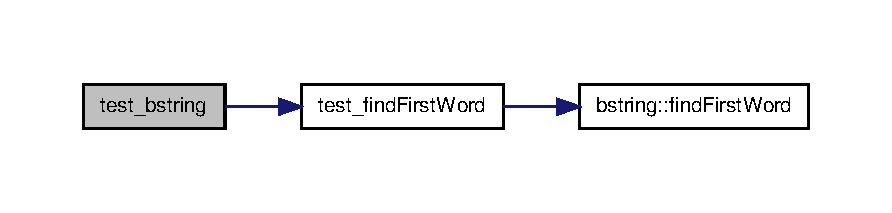
\includegraphics[width=400pt]{bstring_8f90_add6a609edcc15de796d777755c79654b_cgraph}
\end{center}
\end{figure}




Here is the caller graph for this function:
\nopagebreak
\begin{figure}[H]
\begin{center}
\leavevmode
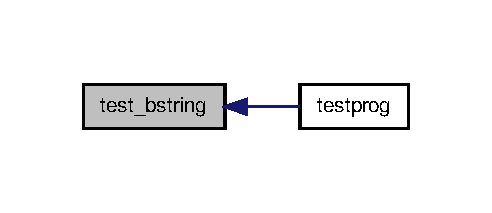
\includegraphics[width=236pt]{bstring_8f90_add6a609edcc15de796d777755c79654b_icgraph}
\end{center}
\end{figure}


\hypertarget{bstring_8f90_ab24d8bc7373b0431185c9c2980035fbb}{
\index{bstring.f90@{bstring.f90}!test\_\-findFirstWord@{test\_\-findFirstWord}}
\index{test\_\-findFirstWord@{test\_\-findFirstWord}!bstring.f90@{bstring.f90}}
\subsubsection[{test\_\-findFirstWord}]{\setlength{\rightskip}{0pt plus 5cm}subroutine test\_\-findFirstWord (
\begin{DoxyParamCaption}
{}
\end{DoxyParamCaption}
)}}
\label{bstring_8f90_ab24d8bc7373b0431185c9c2980035fbb}


Definition at line 122 of file bstring.f90.



Here is the call graph for this function:\nopagebreak
\begin{figure}[H]
\begin{center}
\leavevmode
\includegraphics[width=324pt]{bstring_8f90_ab24d8bc7373b0431185c9c2980035fbb_cgraph}
\end{center}
\end{figure}




Here is the caller graph for this function:
\nopagebreak
\begin{figure}[H]
\begin{center}
\leavevmode
\includegraphics[width=370pt]{bstring_8f90_ab24d8bc7373b0431185c9c2980035fbb_icgraph}
\end{center}
\end{figure}



\hypertarget{class__ArrayList_8f90}{
\section{/home/bob/proj/DEMAGOQUE/work2/trunk/src/class\_\-ArrayList.f90 File Reference}
\label{class__ArrayList_8f90}\index{/home/bob/proj/DEMAGOQUE/work2/trunk/src/class\_\-ArrayList.f90@{/home/bob/proj/DEMAGOQUE/work2/trunk/src/class\_\-ArrayList.f90}}
}
\subsection*{Data Types}
\begin{DoxyCompactItemize}
\item 
type \hyperlink{typeclass__ArrayList_1_1dArrayList}{class\_\-ArrayList::dArrayList}
\end{DoxyCompactItemize}
\subsection*{Modules}
\begin{DoxyCompactItemize}
\item 
module \hyperlink{namespaceclass__ArrayList}{class\_\-ArrayList}
\end{DoxyCompactItemize}
\subsection*{Functions/Subroutines}
\begin{DoxyCompactItemize}
\item 
type(dArrayList) \hyperlink{namespaceclass__ArrayList_a5363f41df7698922433c25c73d02173d}{class\_\-ArrayList::make\_\-dArrayList} (initLength)
\item 
subroutine \hyperlink{namespaceclass__ArrayList_a87eba505c7caff1cf303b9f92182aab2}{class\_\-ArrayList::dArrayList\_\-add} (list, newValue)
\item 
subroutine \hyperlink{namespaceclass__ArrayList_a772b1369610a1b6481ef81093a7ecadf}{class\_\-ArrayList::dArrayList\_\-ensureCapacity} (list, newCapacity)
\item 
real $\ast$8 \hyperlink{namespaceclass__ArrayList_a956a11e0e4778170667c2e90c9097766}{class\_\-ArrayList::dArrayList\_\-get} (list, indix)
\item 
subroutine \hyperlink{namespaceclass__ArrayList_ad92f2ac90292027093572f20b4be9dc6}{class\_\-ArrayList::dArrayList\_\-set} (list, indix, val)
\item 
integer \hyperlink{namespaceclass__ArrayList_a723eb1c041604ffeb1a0434c521de640}{class\_\-ArrayList::dArrayList\_\-size} (list)
\end{DoxyCompactItemize}
\subsection*{Variables}
\begin{DoxyCompactItemize}
\item 
integer, parameter, private \hyperlink{namespaceclass__ArrayList_a710a353a125e9fcbc6bbb0fc3a468afb}{class\_\-ArrayList::INITIAL\_\-LENGTH} = 10
\end{DoxyCompactItemize}

\hypertarget{class__PhysicalQuantity_8f90}{
\section{/home/bob/proj/DEMAGOQUE/work2/trunk/src/class\_\-PhysicalQuantity.f90 File Reference}
\label{class__PhysicalQuantity_8f90}\index{/home/bob/proj/DEMAGOQUE/work2/trunk/src/class\_\-PhysicalQuantity.f90@{/home/bob/proj/DEMAGOQUE/work2/trunk/src/class\_\-PhysicalQuantity.f90}}
}
\subsection*{Data Types}
\begin{DoxyCompactItemize}
\item 
type \hyperlink{typeclass__PhysicalQuantity_1_1PhysicalQuantity}{class\_\-PhysicalQuantity::PhysicalQuantity}
\begin{DoxyCompactList}\small\item\em Stores a quantity with a value, uncertainty, and units. \item\end{DoxyCompactList}\end{DoxyCompactItemize}
\subsection*{Modules}
\begin{DoxyCompactItemize}
\item 
module \hyperlink{namespaceclass__PhysicalQuantity}{class\_\-PhysicalQuantity}
\end{DoxyCompactItemize}
\subsection*{Functions/Subroutines}
\begin{DoxyCompactItemize}
\item 
type(physicalQuantity) \hyperlink{namespaceclass__PhysicalQuantity_a31d0e7291e89fca5b49f9484556cf0cb}{class\_\-PhysicalQuantity::new\_\-PhysicalQuantity} (newSymbol, newDimensions, newVal, newUnc)
\begin{DoxyCompactList}\small\item\em Constructs new \hyperlink{typeclass__PhysicalQuantity_1_1PhysicalQuantity}{PhysicalQuantity}. Assumes the value and uncertainty are given in the current unit system. \item\end{DoxyCompactList}\end{DoxyCompactItemize}
\subsection*{Variables}
\begin{DoxyCompactItemize}
\item 
integer, parameter, private \hyperlink{namespaceclass__PhysicalQuantity_a2870256032bca15f690a32ce1d1b6c52}{class\_\-PhysicalQuantity::MAX\_\-SYMBOL\_\-SIZE} = 5
\item 
type(UnitSystem) \hyperlink{namespaceclass__PhysicalQuantity_a61173098b2362361938556f5fb35431e}{class\_\-PhysicalQuantity::theUnitSystem} = UNIT\_\-SYSTEM\_\-SI
\begin{DoxyCompactList}\small\item\em This is the unit system that all quantities are defined in. By default, we use SI units. \item\end{DoxyCompactList}\item 
type(PhysicalQuantity), parameter \hyperlink{namespaceclass__PhysicalQuantity_a0633cd9b4645d04d7d47dbd151837757}{class\_\-PhysicalQuantity::METER} = PhysicalQuantity(\char`\"{}m\char`\"{}, (/1,0,0,0,0,0,0/), 1, 0)
\item 
type(PhysicalQuantity), parameter \hyperlink{namespaceclass__PhysicalQuantity_a902db03da895ab4c528d71d99e8549b0}{class\_\-PhysicalQuantity::KILOGRAM} = PhysicalQuantity(\char`\"{}kg\char`\"{}, (/0,1,0,0,0,0,0/), 1, 0)
\item 
type(PhysicalQuantity), parameter \hyperlink{namespaceclass__PhysicalQuantity_a7fdf486aace5a1e99af5a634719bb9ce}{class\_\-PhysicalQuantity::SECOND} = PhysicalQuantity(\char`\"{}s\char`\"{}, (/0,0,1,0,0,0,0/), 1, 0)
\item 
type(PhysicalQuantity), parameter \hyperlink{namespaceclass__PhysicalQuantity_a9672ba1ed56d49205a831ba235421de8}{class\_\-PhysicalQuantity::AMPERE} = PhysicalQuantity(\char`\"{}A\char`\"{}, (/0,0,0,1,0,0,0/), 1, 0)
\item 
type(PhysicalQuantity), parameter \hyperlink{namespaceclass__PhysicalQuantity_a2fd77862111da187e89aaf75383baa00}{class\_\-PhysicalQuantity::KELVIN} = PhysicalQuantity(\char`\"{}K\char`\"{}, (/0,0,0,0,1,0,0/), 1, 0)
\item 
type(PhysicalQuantity), parameter \hyperlink{namespaceclass__PhysicalQuantity_a22a20ab491923015030051550a34c977}{class\_\-PhysicalQuantity::MOLE} = PhysicalQuantity(\char`\"{}mol\char`\"{}, (/0,0,0,0,0,1,0/), 1, 0)
\item 
type(PhysicalQuantity), parameter \hyperlink{namespaceclass__PhysicalQuantity_ad332548c0150950850a5fece3ef0e8d2}{class\_\-PhysicalQuantity::CANDELA} = PhysicalQuantity(\char`\"{}cd\char`\"{}, (/0,0,0,0,0,0,1/), 1, 0)
\end{DoxyCompactItemize}

\hypertarget{compareAB_8f90}{
\section{/home/bob/proj/DEMAGOQUE/work2/trunk/src/compareAB.f90 File Reference}
\label{compareAB_8f90}\index{/home/bob/proj/DEMAGOQUE/work2/trunk/src/compareAB.f90@{/home/bob/proj/DEMAGOQUE/work2/trunk/src/compareAB.f90}}
}
\subsection*{Functions/Subroutines}
\begin{DoxyCompactItemize}
\item 
program \hyperlink{compareAB_8f90_a0a7a1ff7db84f05ed049e56a691079dc}{compareAB}
\end{DoxyCompactItemize}


\subsection{Function Documentation}
\hypertarget{compareAB_8f90_a0a7a1ff7db84f05ed049e56a691079dc}{
\index{compareAB.f90@{compareAB.f90}!compareAB@{compareAB}}
\index{compareAB@{compareAB}!compareAB.f90@{compareAB.f90}}
\subsubsection[{compareAB}]{\setlength{\rightskip}{0pt plus 5cm}program compareAB (
\begin{DoxyParamCaption}
{}
\end{DoxyParamCaption}
)}}
\label{compareAB_8f90_a0a7a1ff7db84f05ed049e56a691079dc}


Definition at line 23 of file compareAB.f90.


\hypertarget{cons__laws_8f90}{
\section{/home/bob/proj/DEMAGOQUE/work2/trunk/src/cons\_\-laws.f90 File Reference}
\label{cons__laws_8f90}\index{/home/bob/proj/DEMAGOQUE/work2/trunk/src/cons\_\-laws.f90@{/home/bob/proj/DEMAGOQUE/work2/trunk/src/cons\_\-laws.f90}}
}
\subsection*{Modules}
\begin{DoxyCompactItemize}
\item 
module \hyperlink{namespacecons__laws}{cons\_\-laws}
\end{DoxyCompactItemize}
\subsection*{Variables}
\begin{DoxyCompactItemize}
\item 
real(Long) \hyperlink{namespacecons__laws_a8d6ef7d1726b52d17e21c62607c22c3b}{cons\_\-laws::ekin}
\item 
real(Long) \hyperlink{namespacecons__laws_aaaca27b785c52ee051b7f12c73182924}{cons\_\-laws::ekerr}
\item 
real(Long) \hyperlink{namespacecons__laws_a1a3384f3d97911851a7c728ae1cd8af7}{cons\_\-laws::ek0}
\item 
real(Long) \hyperlink{namespacecons__laws_a2d6e39be272e86946cd52d0596c6bc3a}{cons\_\-laws::ek0err}
\item 
real(Long), dimension(:), allocatable \hyperlink{namespacecons__laws_a5e16e552d92dd5dd52c3cdc8600e62fe}{cons\_\-laws::potx}
\item 
real(Long) \hyperlink{namespacecons__laws_a63e2f83fe00d6af9a68267f70281beac}{cons\_\-laws::epot}
\item 
real(Long) \hyperlink{namespacecons__laws_a1fa58c36c9b57ed4261fddafdadfb924}{cons\_\-laws::eperr}
\item 
real(Long) \hyperlink{namespacecons__laws_a1241ed7a0d2ec35982d18efa725fd588}{cons\_\-laws::ep0}
\item 
real(Long) \hyperlink{namespacecons__laws_a9552ba8aaa6ba5048797e3dcabad3eb4}{cons\_\-laws::ep0err}
\item 
real(Long) \hyperlink{namespacecons__laws_ac8202a23f94b9d534dfc7d5169d2e4bf}{cons\_\-laws::nnum}
\end{DoxyCompactItemize}

\hypertarget{dmtdhf_8f90}{
\section{/home/bob/proj/DEMAGOQUE/work2/trunk/src/dmtdhf.f90 File Reference}
\label{dmtdhf_8f90}\index{/home/bob/proj/DEMAGOQUE/work2/trunk/src/dmtdhf.f90@{/home/bob/proj/DEMAGOQUE/work2/trunk/src/dmtdhf.f90}}
}
\subsection*{Functions/Subroutines}
\begin{DoxyCompactItemize}
\item 
program \hyperlink{dmtdhf_8f90_a4c78fab1fadc6556ab23455891514cc9}{dmtdhf}
\item 
subroutine \hyperlink{dmtdhf_8f90_a4fb412c5e8965afa5aade50b0a65d9ec}{getStdIn}
\end{DoxyCompactItemize}


\subsection{Function Documentation}
\hypertarget{dmtdhf_8f90_a4c78fab1fadc6556ab23455891514cc9}{
\index{dmtdhf.f90@{dmtdhf.f90}!dmtdhf@{dmtdhf}}
\index{dmtdhf@{dmtdhf}!dmtdhf.f90@{dmtdhf.f90}}
\subsubsection[{dmtdhf}]{\setlength{\rightskip}{0pt plus 5cm}program dmtdhf (
\begin{DoxyParamCaption}
{}
\end{DoxyParamCaption}
)}}
\label{dmtdhf_8f90_a4c78fab1fadc6556ab23455891514cc9}


Definition at line 90 of file dmtdhf.f90.



Here is the call graph for this function:\nopagebreak
\begin{figure}[H]
\begin{center}
\leavevmode
\includegraphics[width=400pt]{dmtdhf_8f90_a4c78fab1fadc6556ab23455891514cc9_cgraph}
\end{center}
\end{figure}


\hypertarget{dmtdhf_8f90_a4fb412c5e8965afa5aade50b0a65d9ec}{
\index{dmtdhf.f90@{dmtdhf.f90}!getStdIn@{getStdIn}}
\index{getStdIn@{getStdIn}!dmtdhf.f90@{dmtdhf.f90}}
\subsubsection[{getStdIn}]{\setlength{\rightskip}{0pt plus 5cm}subroutine getStdIn (
\begin{DoxyParamCaption}
{}
\end{DoxyParamCaption}
)}}
\label{dmtdhf_8f90_a4fb412c5e8965afa5aade50b0a65d9ec}


Definition at line 318 of file dmtdhf.f90.



Here is the call graph for this function:\nopagebreak
\begin{figure}[H]
\begin{center}
\leavevmode
\includegraphics[width=400pt]{dmtdhf_8f90_a4fb412c5e8965afa5aade50b0a65d9ec_cgraph}
\end{center}
\end{figure}




Here is the caller graph for this function:
\nopagebreak
\begin{figure}[H]
\begin{center}
\leavevmode
\includegraphics[width=218pt]{dmtdhf_8f90_a4fb412c5e8965afa5aade50b0a65d9ec_icgraph}
\end{center}
\end{figure}



\hypertarget{ener_8f90}{
\section{/home/bob/proj/DEMAGOQUE/work2/trunk/src/ener.f90 File Reference}
\label{ener_8f90}\index{/home/bob/proj/DEMAGOQUE/work2/trunk/src/ener.f90@{/home/bob/proj/DEMAGOQUE/work2/trunk/src/ener.f90}}
}
\subsection*{Functions/Subroutines}
\begin{DoxyCompactItemize}
\item 
subroutine \hyperlink{ener_8f90_af156f82211a41e497139422d1a7c2807}{ener\_\-k}
\item 
subroutine \hyperlink{ener_8f90_a498d75d5ca779f099334f41509d7592a}{ener\_\-x}
\end{DoxyCompactItemize}


\subsection{Function Documentation}
\hypertarget{ener_8f90_af156f82211a41e497139422d1a7c2807}{
\index{ener.f90@{ener.f90}!ener\_\-k@{ener\_\-k}}
\index{ener\_\-k@{ener\_\-k}!ener.f90@{ener.f90}}
\subsubsection[{ener\_\-k}]{\setlength{\rightskip}{0pt plus 5cm}subroutine ener\_\-k (
\begin{DoxyParamCaption}
{}
\end{DoxyParamCaption}
)}}
\label{ener_8f90_af156f82211a41e497139422d1a7c2807}


Definition at line 23 of file ener.f90.



Here is the call graph for this function:\nopagebreak
\begin{figure}[H]
\begin{center}
\leavevmode
\includegraphics[width=400pt]{ener_8f90_af156f82211a41e497139422d1a7c2807_cgraph}
\end{center}
\end{figure}




Here is the caller graph for this function:
\nopagebreak
\begin{figure}[H]
\begin{center}
\leavevmode
\includegraphics[width=400pt]{ener_8f90_af156f82211a41e497139422d1a7c2807_icgraph}
\end{center}
\end{figure}


\hypertarget{ener_8f90_a498d75d5ca779f099334f41509d7592a}{
\index{ener.f90@{ener.f90}!ener\_\-x@{ener\_\-x}}
\index{ener\_\-x@{ener\_\-x}!ener.f90@{ener.f90}}
\subsubsection[{ener\_\-x}]{\setlength{\rightskip}{0pt plus 5cm}subroutine ener\_\-x (
\begin{DoxyParamCaption}
{}
\end{DoxyParamCaption}
)}}
\label{ener_8f90_a498d75d5ca779f099334f41509d7592a}


Definition at line 68 of file ener.f90.



Here is the call graph for this function:\nopagebreak
\begin{figure}[H]
\begin{center}
\leavevmode
\includegraphics[width=400pt]{ener_8f90_a498d75d5ca779f099334f41509d7592a_cgraph}
\end{center}
\end{figure}




Here is the caller graph for this function:
\nopagebreak
\begin{figure}[H]
\begin{center}
\leavevmode
\includegraphics[width=400pt]{ener_8f90_a498d75d5ca779f099334f41509d7592a_icgraph}
\end{center}
\end{figure}



\hypertarget{fft__nag_8f90}{
\section{/home/bob/proj/DEMAGOQUE/work2/trunk/src/fft\_\-nag.f90 File Reference}
\label{fft__nag_8f90}\index{/home/bob/proj/DEMAGOQUE/work2/trunk/src/fft\_\-nag.f90@{/home/bob/proj/DEMAGOQUE/work2/trunk/src/fft\_\-nag.f90}}
}
\subsection*{Functions/Subroutines}
\begin{DoxyCompactItemize}
\item 
subroutine \hyperlink{fft__nag_8f90_a89e00c863f191d838efd7dda883a632a}{FT} (Nx, Ny, xre, xim)
\item 
subroutine \hyperlink{fft__nag_8f90_a4843ff1b354998a8e8fea9af783a4f59}{IFT} (Nx, Ny, xre, xim)
\end{DoxyCompactItemize}


\subsection{Function Documentation}
\hypertarget{fft__nag_8f90_a89e00c863f191d838efd7dda883a632a}{
\index{fft\_\-nag.f90@{fft\_\-nag.f90}!FT@{FT}}
\index{FT@{FT}!fft_nag.f90@{fft\_\-nag.f90}}
\subsubsection[{FT}]{\setlength{\rightskip}{0pt plus 5cm}subroutine FT (
\begin{DoxyParamCaption}
\item[{integer}]{Nx, }
\item[{integer}]{Ny, }
\item[{real (Long),dimension(nx,ny)}]{xre, }
\item[{real (Long),dimension(nx,ny)}]{xim}
\end{DoxyParamCaption}
)}}
\label{fft__nag_8f90_a89e00c863f191d838efd7dda883a632a}


Definition at line 8 of file fft\_\-nag.f90.



Here is the caller graph for this function:
\nopagebreak
\begin{figure}[H]
\begin{center}
\leavevmode
\includegraphics[width=188pt]{fft__nag_8f90_a89e00c863f191d838efd7dda883a632a_icgraph}
\end{center}
\end{figure}


\hypertarget{fft__nag_8f90_a4843ff1b354998a8e8fea9af783a4f59}{
\index{fft\_\-nag.f90@{fft\_\-nag.f90}!IFT@{IFT}}
\index{IFT@{IFT}!fft_nag.f90@{fft\_\-nag.f90}}
\subsubsection[{IFT}]{\setlength{\rightskip}{0pt plus 5cm}subroutine IFT (
\begin{DoxyParamCaption}
\item[{integer}]{Nx, }
\item[{integer}]{Ny, }
\item[{real (Long),dimension(nx,ny)}]{xre, }
\item[{real (Long),dimension(nx,ny)}]{xim}
\end{DoxyParamCaption}
)}}
\label{fft__nag_8f90_a4843ff1b354998a8e8fea9af783a4f59}


Definition at line 62 of file fft\_\-nag.f90.


\hypertarget{format_8f90}{
\section{/home/bob/proj/DEMAGOQUE/work2/trunk/src/format.f90 File Reference}
\label{format_8f90}\index{/home/bob/proj/DEMAGOQUE/work2/trunk/src/format.f90@{/home/bob/proj/DEMAGOQUE/work2/trunk/src/format.f90}}
}
\subsection*{Modules}
\begin{DoxyCompactItemize}
\item 
module \hyperlink{namespaceformat}{format}
\end{DoxyCompactItemize}
\subsection*{Variables}
\begin{DoxyCompactItemize}
\item 
integer \hyperlink{namespaceformat_a35a6cb9f260951fd6bd7ba9144cfaf5e}{format::dummy}
\end{DoxyCompactItemize}

\hypertarget{formatting_8f90}{
\section{/home/bob/proj/DEMAGOQUE/work2/trunk/src/formatting.f90 File Reference}
\label{formatting_8f90}\index{/home/bob/proj/DEMAGOQUE/work2/trunk/src/formatting.f90@{/home/bob/proj/DEMAGOQUE/work2/trunk/src/formatting.f90}}
}
\subsection*{Modules}
\begin{DoxyCompactItemize}
\item 
module \hyperlink{namespaceformatting}{formatting}
\end{DoxyCompactItemize}
\subsection*{Variables}
\begin{DoxyCompactItemize}
\item 
character(len=20), parameter \hyperlink{namespaceformatting_a552aa51d2fb15a338e371114fd02c6e1}{formatting::fr5} = \char`\"{}(5E17.9)\char`\"{}
\end{DoxyCompactItemize}

\hypertarget{initial_8f90}{
\section{/home/bob/proj/DEMAGOQUE/work2/trunk/src/initial.f90 File Reference}
\label{initial_8f90}\index{/home/bob/proj/DEMAGOQUE/work2/trunk/src/initial.f90@{/home/bob/proj/DEMAGOQUE/work2/trunk/src/initial.f90}}
}
\subsection*{Functions/Subroutines}
\begin{DoxyCompactItemize}
\item 
subroutine \hyperlink{initial_8f90_aa52194698c8a672712fb4bf627fdf0e2}{calcInitial}
\item 
subroutine \hyperlink{initial_8f90_ae3fd441fd7d3cf3f49c5745a9f496b1a}{initialState}
\item 
subroutine \hyperlink{initial_8f90_aa3d543e8caceb0c26b94720e00c38e61}{copyExtra}
\item 
subroutine \hyperlink{initial_8f90_af10aed743d4a9864da67c314b2ccd0f6}{boost}
\item 
subroutine \hyperlink{initial_8f90_a8febc15c68033c55e7f246e07e193ed3}{displaceLeft} (nx)
\item 
subroutine \hyperlink{initial_8f90_af0a399573512e92199bb43c56efa632b}{displaceRight} (nx)
\item 
subroutine \hyperlink{initial_8f90_a2efc6884e391e25a879a5231eeda9956}{flipclone}
\item 
subroutine \hyperlink{initial_8f90_a00ff7d260d65e323892041631c2343bc}{getX12} (ixa, ixr, x1, x2)
\item 
subroutine \hyperlink{initial_8f90_aa274d8457716dc63d8ed63a03a880a19}{getrX12} (xa1, xr1, x1, x2)
\item 
subroutine \hyperlink{initial_8f90_a95f93172bd89ed6a8d446e339f217cef}{getK12} (ika, ikr, k1, k2)
\end{DoxyCompactItemize}


\subsection{Function Documentation}
\hypertarget{initial_8f90_af10aed743d4a9864da67c314b2ccd0f6}{
\index{initial.f90@{initial.f90}!boost@{boost}}
\index{boost@{boost}!initial.f90@{initial.f90}}
\subsubsection[{boost}]{\setlength{\rightskip}{0pt plus 5cm}subroutine boost (
\begin{DoxyParamCaption}
{}
\end{DoxyParamCaption}
)}}
\label{initial_8f90_af10aed743d4a9864da67c314b2ccd0f6}


Definition at line 186 of file initial.f90.



Here is the call graph for this function:\nopagebreak
\begin{figure}[H]
\begin{center}
\leavevmode
\includegraphics[width=400pt]{initial_8f90_af10aed743d4a9864da67c314b2ccd0f6_cgraph}
\end{center}
\end{figure}




Here is the caller graph for this function:
\nopagebreak
\begin{figure}[H]
\begin{center}
\leavevmode
\includegraphics[width=206pt]{initial_8f90_af10aed743d4a9864da67c314b2ccd0f6_icgraph}
\end{center}
\end{figure}


\hypertarget{initial_8f90_aa52194698c8a672712fb4bf627fdf0e2}{
\index{initial.f90@{initial.f90}!calcInitial@{calcInitial}}
\index{calcInitial@{calcInitial}!initial.f90@{initial.f90}}
\subsubsection[{calcInitial}]{\setlength{\rightskip}{0pt plus 5cm}subroutine calcInitial (
\begin{DoxyParamCaption}
{}
\end{DoxyParamCaption}
)}}
\label{initial_8f90_aa52194698c8a672712fb4bf627fdf0e2}


Definition at line 25 of file initial.f90.



Here is the call graph for this function:\nopagebreak
\begin{figure}[H]
\begin{center}
\leavevmode
\includegraphics[width=280pt]{initial_8f90_aa52194698c8a672712fb4bf627fdf0e2_cgraph}
\end{center}
\end{figure}




Here is the caller graph for this function:
\nopagebreak
\begin{figure}[H]
\begin{center}
\leavevmode
\includegraphics[width=222pt]{initial_8f90_aa52194698c8a672712fb4bf627fdf0e2_icgraph}
\end{center}
\end{figure}


\hypertarget{initial_8f90_aa3d543e8caceb0c26b94720e00c38e61}{
\index{initial.f90@{initial.f90}!copyExtra@{copyExtra}}
\index{copyExtra@{copyExtra}!initial.f90@{initial.f90}}
\subsubsection[{copyExtra}]{\setlength{\rightskip}{0pt plus 5cm}subroutine copyExtra (
\begin{DoxyParamCaption}
{}
\end{DoxyParamCaption}
)}}
\label{initial_8f90_aa3d543e8caceb0c26b94720e00c38e61}


Definition at line 141 of file initial.f90.



Here is the caller graph for this function:
\nopagebreak
\begin{figure}[H]
\begin{center}
\leavevmode
\includegraphics[width=400pt]{initial_8f90_aa3d543e8caceb0c26b94720e00c38e61_icgraph}
\end{center}
\end{figure}


\hypertarget{initial_8f90_a8febc15c68033c55e7f246e07e193ed3}{
\index{initial.f90@{initial.f90}!displaceLeft@{displaceLeft}}
\index{displaceLeft@{displaceLeft}!initial.f90@{initial.f90}}
\subsubsection[{displaceLeft}]{\setlength{\rightskip}{0pt plus 5cm}subroutine displaceLeft (
\begin{DoxyParamCaption}
\item[{integer,intent(in)}]{nx}
\end{DoxyParamCaption}
)}}
\label{initial_8f90_a8febc15c68033c55e7f246e07e193ed3}


Definition at line 254 of file initial.f90.



Here is the caller graph for this function:
\nopagebreak
\begin{figure}[H]
\begin{center}
\leavevmode
\includegraphics[width=234pt]{initial_8f90_a8febc15c68033c55e7f246e07e193ed3_icgraph}
\end{center}
\end{figure}


\hypertarget{initial_8f90_af0a399573512e92199bb43c56efa632b}{
\index{initial.f90@{initial.f90}!displaceRight@{displaceRight}}
\index{displaceRight@{displaceRight}!initial.f90@{initial.f90}}
\subsubsection[{displaceRight}]{\setlength{\rightskip}{0pt plus 5cm}subroutine displaceRight (
\begin{DoxyParamCaption}
\item[{integer,intent(in)}]{nx}
\end{DoxyParamCaption}
)}}
\label{initial_8f90_af0a399573512e92199bb43c56efa632b}


Definition at line 284 of file initial.f90.



Here is the caller graph for this function:
\nopagebreak
\begin{figure}[H]
\begin{center}
\leavevmode
\includegraphics[width=240pt]{initial_8f90_af0a399573512e92199bb43c56efa632b_icgraph}
\end{center}
\end{figure}


\hypertarget{initial_8f90_a2efc6884e391e25a879a5231eeda9956}{
\index{initial.f90@{initial.f90}!flipclone@{flipclone}}
\index{flipclone@{flipclone}!initial.f90@{initial.f90}}
\subsubsection[{flipclone}]{\setlength{\rightskip}{0pt plus 5cm}subroutine flipclone (
\begin{DoxyParamCaption}
{}
\end{DoxyParamCaption}
)}}
\label{initial_8f90_a2efc6884e391e25a879a5231eeda9956}


Definition at line 316 of file initial.f90.



Here is the call graph for this function:\nopagebreak
\begin{figure}[H]
\begin{center}
\leavevmode
\includegraphics[width=232pt]{initial_8f90_a2efc6884e391e25a879a5231eeda9956_cgraph}
\end{center}
\end{figure}




Here is the caller graph for this function:
\nopagebreak
\begin{figure}[H]
\begin{center}
\leavevmode
\includegraphics[width=218pt]{initial_8f90_a2efc6884e391e25a879a5231eeda9956_icgraph}
\end{center}
\end{figure}


\hypertarget{initial_8f90_a95f93172bd89ed6a8d446e339f217cef}{
\index{initial.f90@{initial.f90}!getK12@{getK12}}
\index{getK12@{getK12}!initial.f90@{initial.f90}}
\subsubsection[{getK12}]{\setlength{\rightskip}{0pt plus 5cm}subroutine getK12 (
\begin{DoxyParamCaption}
\item[{integer,intent(in)}]{ika, }
\item[{integer,intent(in)}]{ikr, }
\item[{real$\ast$8,intent(out)}]{k1, }
\item[{real$\ast$8,intent(out)}]{k2}
\end{DoxyParamCaption}
)}}
\label{initial_8f90_a95f93172bd89ed6a8d446e339f217cef}


Definition at line 443 of file initial.f90.



Here is the caller graph for this function:
\nopagebreak
\begin{figure}[H]
\begin{center}
\leavevmode
\includegraphics[width=400pt]{initial_8f90_a95f93172bd89ed6a8d446e339f217cef_icgraph}
\end{center}
\end{figure}


\hypertarget{initial_8f90_aa274d8457716dc63d8ed63a03a880a19}{
\index{initial.f90@{initial.f90}!getrX12@{getrX12}}
\index{getrX12@{getrX12}!initial.f90@{initial.f90}}
\subsubsection[{getrX12}]{\setlength{\rightskip}{0pt plus 5cm}subroutine getrX12 (
\begin{DoxyParamCaption}
\item[{real$\ast$8,intent(in)}]{xa1, }
\item[{real$\ast$8,intent(in)}]{xr1, }
\item[{real$\ast$8,intent(out)}]{x1, }
\item[{real$\ast$8,intent(out)}]{x2}
\end{DoxyParamCaption}
)}}
\label{initial_8f90_aa274d8457716dc63d8ed63a03a880a19}


Definition at line 422 of file initial.f90.



Here is the caller graph for this function:
\nopagebreak
\begin{figure}[H]
\begin{center}
\leavevmode
\includegraphics[width=400pt]{initial_8f90_aa274d8457716dc63d8ed63a03a880a19_icgraph}
\end{center}
\end{figure}


\hypertarget{initial_8f90_a00ff7d260d65e323892041631c2343bc}{
\index{initial.f90@{initial.f90}!getX12@{getX12}}
\index{getX12@{getX12}!initial.f90@{initial.f90}}
\subsubsection[{getX12}]{\setlength{\rightskip}{0pt plus 5cm}subroutine getX12 (
\begin{DoxyParamCaption}
\item[{integer,intent(in)}]{ixa, }
\item[{integer,intent(in)}]{ixr, }
\item[{real (Long),intent(out)}]{x1, }
\item[{real (Long),intent(out)}]{x2}
\end{DoxyParamCaption}
)}}
\label{initial_8f90_a00ff7d260d65e323892041631c2343bc}


Definition at line 392 of file initial.f90.



Here is the call graph for this function:\nopagebreak
\begin{figure}[H]
\begin{center}
\leavevmode
\includegraphics[width=214pt]{initial_8f90_a00ff7d260d65e323892041631c2343bc_cgraph}
\end{center}
\end{figure}




Here is the caller graph for this function:
\nopagebreak
\begin{figure}[H]
\begin{center}
\leavevmode
\includegraphics[width=400pt]{initial_8f90_a00ff7d260d65e323892041631c2343bc_icgraph}
\end{center}
\end{figure}


\hypertarget{initial_8f90_ae3fd441fd7d3cf3f49c5745a9f496b1a}{
\index{initial.f90@{initial.f90}!initialState@{initialState}}
\index{initialState@{initialState}!initial.f90@{initial.f90}}
\subsubsection[{initialState}]{\setlength{\rightskip}{0pt plus 5cm}subroutine initialState (
\begin{DoxyParamCaption}
{}
\end{DoxyParamCaption}
)}}
\label{initial_8f90_ae3fd441fd7d3cf3f49c5745a9f496b1a}


Definition at line 50 of file initial.f90.



Here is the call graph for this function:\nopagebreak
\begin{figure}[H]
\begin{center}
\leavevmode
\includegraphics[width=390pt]{initial_8f90_ae3fd441fd7d3cf3f49c5745a9f496b1a_cgraph}
\end{center}
\end{figure}




Here is the caller graph for this function:
\nopagebreak
\begin{figure}[H]
\begin{center}
\leavevmode
\includegraphics[width=226pt]{initial_8f90_ae3fd441fd7d3cf3f49c5745a9f496b1a_icgraph}
\end{center}
\end{figure}



\hypertarget{input__parameters_8f90}{
\section{/home/bob/proj/DEMAGOQUE/work2/trunk/src/input\_\-parameters.f90 File Reference}
\label{input__parameters_8f90}\index{/home/bob/proj/DEMAGOQUE/work2/trunk/src/input\_\-parameters.f90@{/home/bob/proj/DEMAGOQUE/work2/trunk/src/input\_\-parameters.f90}}
}
\subsection*{Modules}
\begin{DoxyCompactItemize}
\item 
module \hyperlink{namespaceinput__parameters}{input\_\-parameters}
\end{DoxyCompactItemize}
\subsection*{Variables}
\begin{DoxyCompactItemize}
\item 
integer \hyperlink{namespaceinput__parameters_a27dbda031851f558814121445cf46ed9}{input\_\-parameters::potInitial}
\item 
integer \hyperlink{namespaceinput__parameters_a2ccc9d711d290b3e33fbc675ed390af2}{input\_\-parameters::potFinal}
\item 
real(Long) \hyperlink{namespaceinput__parameters_ac937498371c0568d2d4ed1e1ef034e1d}{input\_\-parameters::ea}
\item 
integer \hyperlink{namespaceinput__parameters_a0c5bab2cbe910c8543c442cb9be582d0}{input\_\-parameters::ntime}
\item 
REAL(Long) \hyperlink{namespaceinput__parameters_a42efff37bd453975f48e8485e5757acd}{input\_\-parameters::delt}
\item 
integer \hyperlink{namespaceinput__parameters_a3db2ebb8fcd24f403d0c3bd05a38e4c2}{input\_\-parameters::Nevt}
\item 
logical \hyperlink{namespaceinput__parameters_aa73f50863135132e72d9a9c93d2cadef}{input\_\-parameters::useImCutoff}
\item 
real(Long) \hyperlink{namespaceinput__parameters_a3987174aef89a10227220b4e5bdecde6}{input\_\-parameters::cutoff\_\-w0}
\item 
real(Long) \hyperlink{namespaceinput__parameters_a87f2d307b48a20f985ea0692b9dfebf6}{input\_\-parameters::cutoff\_\-x0}
\item 
real(Long) \hyperlink{namespaceinput__parameters_a8e63bceb853ebd1124eda12568a0e57f}{input\_\-parameters::cutoff\_\-d0}
\item 
real(Long) \hyperlink{namespaceinput__parameters_a1d8bbaa8b473b798cb43170831cc57ac}{input\_\-parameters::initialSeparation}
\item 
logical \hyperlink{namespaceinput__parameters_add8bfc502078fcdca67fff41e00114f7}{input\_\-parameters::initState\_\-gaussianNuclear}
\item 
REAL(long) \hyperlink{namespaceinput__parameters_a745c6398e72faacdaacba0cf01027565}{input\_\-parameters::w}
\item 
REAL(long) \hyperlink{namespaceinput__parameters_ae3a25357531dd0d2b8c5c4cc2de073d9}{input\_\-parameters::whm}
\item 
INTEGER \hyperlink{namespaceinput__parameters_a29545f09a06c5a3def5df7fdb5f966ab}{input\_\-parameters::Nmax}
\item 
logical \hyperlink{namespaceinput__parameters_a794b8486b7ecd6258448887bce533681}{input\_\-parameters::initState\_\-cosine}
\item 
integer \hyperlink{namespaceinput__parameters_ad5ff3d9c110be99ed08bbe970f1630c8}{input\_\-parameters::initState\_\-cosine\_\-number}
\item 
real(Long) \hyperlink{namespaceinput__parameters_a51d2cc916f531fadef1a6f0729644174}{input\_\-parameters::initState\_\-cosine\_\-norm}
\item 
real(Long) \hyperlink{namespaceinput__parameters_ac3a5530df841dc82b4819f34f1e44980}{input\_\-parameters::initState\_\-cosine\_\-shift}
\item 
logical \hyperlink{namespaceinput__parameters_a727a13be305b5dde7955fd2d02f955e4}{input\_\-parameters::initState\_\-plane}
\item 
integer \hyperlink{namespaceinput__parameters_a876ac6edc93b733aeb66f54aca167741}{input\_\-parameters::initState\_\-plane\_\-number}
\item 
real(Long) \hyperlink{namespaceinput__parameters_a22ba3f1343580a0db34433e32279e365}{input\_\-parameters::initState\_\-plane\_\-norm}
\item 
real(Long) \hyperlink{namespaceinput__parameters_a97253a3c66d919b8a99dd33c633d3bd8}{input\_\-parameters::initState\_\-plane\_\-shift}
\item 
logical \hyperlink{namespaceinput__parameters_aae45dd03716b9ad9a0600a9d9a798935}{input\_\-parameters::initState\_\-kdelta}
\item 
real(Long) \hyperlink{namespaceinput__parameters_a1b2e5c088ab1d39d896586d7fb18b142}{input\_\-parameters::initState\_\-kdelta\_\-norm}
\item 
real(Long) \hyperlink{namespaceinput__parameters_a65eb9165c6a1fd054daefc2a96e7ae2a}{input\_\-parameters::initState\_\-kdelta\_\-x0}
\item 
integer \hyperlink{namespaceinput__parameters_a127f71f45eade1f05ced1535e88c771d}{input\_\-parameters::splitOperatorMethod}
\item 
logical \hyperlink{namespaceinput__parameters_a716cb07ce1fca722dacc327ddc4011fd}{input\_\-parameters::unitSystem\_\-bec}
\begin{DoxyCompactList}\small\item\em Use unit system for Bose-\/Einstein Condensate. \item\end{DoxyCompactList}\item 
logical \hyperlink{namespaceinput__parameters_a65ef9c71ef768c5f3b871cae9143108e}{input\_\-parameters::unitSystem\_\-nuclear}
\begin{DoxyCompactList}\small\item\em Use unit system for nuclear collision \mbox{[}default\mbox{]}. \item\end{DoxyCompactList}\item 
logical \hyperlink{namespaceinput__parameters_a9672a1c90e65a2ecee350dd2dae64e03}{input\_\-parameters::useImEvol}
\item 
integer \hyperlink{namespaceinput__parameters_ac0212885e38ab22a77411b20bec16420}{input\_\-parameters::Nimev}
\item 
logical \hyperlink{namespaceinput__parameters_a504b6e2c93e4a4af47125d83d6e5d75d}{input\_\-parameters::useFlipClone}
\item 
logical \hyperlink{namespaceinput__parameters_ac1165234d614ad278effaf2a7910888b}{input\_\-parameters::useAdiabatic}
\item 
integer \hyperlink{namespaceinput__parameters_a2b1e4d8baaa62168d989002cf747b30b}{input\_\-parameters::iadib}
\item 
integer \hyperlink{namespaceinput__parameters_a6e8306262594749651ff9230cb525363}{input\_\-parameters::Nad}
\item 
real(Long) \hyperlink{namespaceinput__parameters_ab3ac3c45168fc6aafd02e70822154417}{input\_\-parameters::tad}
\item 
real(Long) \hyperlink{namespaceinput__parameters_a8d452c8a3d45ee77279fc26867c74ed6}{input\_\-parameters::wtad}
\end{DoxyCompactItemize}

\hypertarget{integra_8f90}{
\section{/home/bob/proj/DEMAGOQUE/work2/trunk/src/integra.f90 File Reference}
\label{integra_8f90}\index{/home/bob/proj/DEMAGOQUE/work2/trunk/src/integra.f90@{/home/bob/proj/DEMAGOQUE/work2/trunk/src/integra.f90}}
}
\subsection*{Functions/Subroutines}
\begin{DoxyCompactItemize}
\item 
subroutine \hyperlink{integra_8f90_a910e7bf7506381bc04bc6ce606870d79}{dint\_\-simp1} (n, f, h, sum, err)
\end{DoxyCompactItemize}


\subsection{Function Documentation}
\hypertarget{integra_8f90_a910e7bf7506381bc04bc6ce606870d79}{
\index{integra.f90@{integra.f90}!dint\_\-simp1@{dint\_\-simp1}}
\index{dint\_\-simp1@{dint\_\-simp1}!integra.f90@{integra.f90}}
\subsubsection[{dint\_\-simp1}]{\setlength{\rightskip}{0pt plus 5cm}subroutine dint\_\-simp1 (
\begin{DoxyParamCaption}
\item[{INTEGER,intent(in)}]{n, }
\item[{REAL (Long),dimension(n),intent(in)}]{f, }
\item[{REAL (Long),intent(in)}]{h, }
\item[{REAL (Long),intent(out)}]{sum, }
\item[{REAL (Long),intent(out)}]{err}
\end{DoxyParamCaption}
)}}
\label{integra_8f90_a910e7bf7506381bc04bc6ce606870d79}


Definition at line 1 of file integra.f90.



Here is the caller graph for this function:\nopagebreak
\begin{figure}[H]
\begin{center}
\leavevmode
\includegraphics[width=224pt]{integra_8f90_a910e7bf7506381bc04bc6ce606870d79_icgraph}
\end{center}
\end{figure}



\hypertarget{interp_8f}{
\section{/home/bob/proj/DEMAGOQUE/work2/trunk/src/interp.f File Reference}
\label{interp_8f}\index{/home/bob/proj/DEMAGOQUE/work2/trunk/src/interp.f@{/home/bob/proj/DEMAGOQUE/work2/trunk/src/interp.f}}
}
\subsection*{Functions/Subroutines}
\begin{DoxyCompactItemize}
\item 
subroutine \hyperlink{interp_8f_abdd2871e2a0a60f37b574156132f426e}{SPLINE} (x, y, n, yp1, ypn, y2)
\item 
subroutine \hyperlink{interp_8f_ac695724b79eba38b0ed89b0268254382}{SPLINT} (xa, ya, y2a, n, x, y)
\item 
subroutine \hyperlink{interp_8f_a6d2236727e8370221917db234bdb42d7}{SPLIN2} (xa, ya, y2a, n, x, y, ki)
\item 
subroutine \hyperlink{interp_8f_aab8bc44fbf2bc0a54fe1bede6c67e78c}{SPINT} (xa, ya, na, xb, yb, nb)
\item 
subroutine \hyperlink{interp_8f_a19542a5a1d6e24681eecb910e9fb52c4}{LIN\_\-INT} (xa, ya, n, x, y, ki)
\item 
subroutine \hyperlink{interp_8f_a96fbad33968d82463f23d2c190c88f11}{LININT} (xa, ya, na, xb, yb, nb)
\item 
subroutine \hyperlink{interp_8f_aa99dd4561dd3b8f55a705bd59376667b}{LIN\_\-INT2D} (xa, nx, ya, ny, za, x, y, z, kx, ky)
\item 
subroutine \hyperlink{interp_8f_ae9e51899edbd82115b64a0df7c7fa0ae}{SPLINE2D} (nx, ya, ny, za, z2a)
\item 
subroutine \hyperlink{interp_8f_ab74c654ddadc3450859b976c50103b84}{SPLINT2D} (xa, nx, ya, ny, za, z2a, xf, yf, zf)
\item 
subroutine \hyperlink{interp_8f_a03815de6282880a4a0126771609fe1e6}{POL\_\-INT} (xa, ya, n, Npol, x, y, dy, nchng, ki)
\item 
subroutine \hyperlink{interp_8f_ad96c0747e78d542397c8834eab85465d}{POLINT} (xa, ya, n, x, y, dy)
\end{DoxyCompactItemize}


\subsection{Function Documentation}
\hypertarget{interp_8f_a19542a5a1d6e24681eecb910e9fb52c4}{
\index{interp.f@{interp.f}!LIN\_\-INT@{LIN\_\-INT}}
\index{LIN\_\-INT@{LIN\_\-INT}!interp.f@{interp.f}}
\subsubsection[{LIN\_\-INT}]{\setlength{\rightskip}{0pt plus 5cm}subroutine LIN\_\-INT (
\begin{DoxyParamCaption}
\item[{DOUBLE PRECISION,dimension(n)}]{xa, }
\item[{DOUBLE PRECISION,dimension(n)}]{ya, }
\item[{INTEGER}]{n, }
\item[{DOUBLE PRECISION}]{x, }
\item[{DOUBLE PRECISION}]{y, }
\item[{INTEGER}]{ki}
\end{DoxyParamCaption}
)}}
\label{interp_8f_a19542a5a1d6e24681eecb910e9fb52c4}


Definition at line 161 of file interp.f.



Here is the caller graph for this function:\nopagebreak
\begin{figure}[H]
\begin{center}
\leavevmode
\includegraphics[width=400pt]{interp_8f_a19542a5a1d6e24681eecb910e9fb52c4_icgraph}
\end{center}
\end{figure}


\hypertarget{interp_8f_aa99dd4561dd3b8f55a705bd59376667b}{
\index{interp.f@{interp.f}!LIN\_\-INT2D@{LIN\_\-INT2D}}
\index{LIN\_\-INT2D@{LIN\_\-INT2D}!interp.f@{interp.f}}
\subsubsection[{LIN\_\-INT2D}]{\setlength{\rightskip}{0pt plus 5cm}subroutine LIN\_\-INT2D (
\begin{DoxyParamCaption}
\item[{DOUBLE PRECISION,dimension(nx)}]{xa, }
\item[{INTEGER}]{nx, }
\item[{DOUBLE PRECISION,dimension(ny)}]{ya, }
\item[{INTEGER}]{ny, }
\item[{DOUBLE PRECISION,dimension(nx,ny)}]{za, }
\item[{DOUBLE PRECISION}]{x, }
\item[{DOUBLE PRECISION}]{y, }
\item[{DOUBLE PRECISION}]{z, }
\item[{INTEGER}]{kx, }
\item[{INTEGER}]{ky}
\end{DoxyParamCaption}
)}}
\label{interp_8f_aa99dd4561dd3b8f55a705bd59376667b}


Definition at line 231 of file interp.f.

\hypertarget{interp_8f_a96fbad33968d82463f23d2c190c88f11}{
\index{interp.f@{interp.f}!LININT@{LININT}}
\index{LININT@{LININT}!interp.f@{interp.f}}
\subsubsection[{LININT}]{\setlength{\rightskip}{0pt plus 5cm}subroutine LININT (
\begin{DoxyParamCaption}
\item[{DOUBLE PRECISION,dimension(na)}]{xa, }
\item[{DOUBLE PRECISION,dimension(na)}]{ya, }
\item[{INTEGER}]{na, }
\item[{DOUBLE PRECISION,dimension(nb)}]{xb, }
\item[{DOUBLE PRECISION,dimension(nb)}]{yb, }
\item[{INTEGER}]{nb}
\end{DoxyParamCaption}
)}}
\label{interp_8f_a96fbad33968d82463f23d2c190c88f11}


Definition at line 214 of file interp.f.

\hypertarget{interp_8f_a03815de6282880a4a0126771609fe1e6}{
\index{interp.f@{interp.f}!POL\_\-INT@{POL\_\-INT}}
\index{POL\_\-INT@{POL\_\-INT}!interp.f@{interp.f}}
\subsubsection[{POL\_\-INT}]{\setlength{\rightskip}{0pt plus 5cm}subroutine POL\_\-INT (
\begin{DoxyParamCaption}
\item[{DOUBLE PRECISION,dimension(n)}]{xa, }
\item[{DOUBLE PRECISION,dimension(n)}]{ya, }
\item[{INTEGER}]{n, }
\item[{INTEGER}]{Npol, }
\item[{DOUBLE PRECISION}]{x, }
\item[{DOUBLE PRECISION}]{y, }
\item[{DOUBLE PRECISION}]{dy, }
\item[{INTEGER}]{nchng, }
\item[{INTEGER}]{ki}
\end{DoxyParamCaption}
)}}
\label{interp_8f_a03815de6282880a4a0126771609fe1e6}


Definition at line 388 of file interp.f.

\hypertarget{interp_8f_ad96c0747e78d542397c8834eab85465d}{
\index{interp.f@{interp.f}!POLINT@{POLINT}}
\index{POLINT@{POLINT}!interp.f@{interp.f}}
\subsubsection[{POLINT}]{\setlength{\rightskip}{0pt plus 5cm}subroutine POLINT (
\begin{DoxyParamCaption}
\item[{DOUBLE PRECISION,dimension(n)}]{xa, }
\item[{DOUBLE PRECISION,dimension(n)}]{ya, }
\item[{INTEGER}]{n, }
\item[{DOUBLE PRECISION}]{x, }
\item[{DOUBLE PRECISION}]{y, }
\item[{DOUBLE PRECISION}]{dy}
\end{DoxyParamCaption}
)}}
\label{interp_8f_ad96c0747e78d542397c8834eab85465d}


Definition at line 456 of file interp.f.

\hypertarget{interp_8f_aab8bc44fbf2bc0a54fe1bede6c67e78c}{
\index{interp.f@{interp.f}!SPINT@{SPINT}}
\index{SPINT@{SPINT}!interp.f@{interp.f}}
\subsubsection[{SPINT}]{\setlength{\rightskip}{0pt plus 5cm}subroutine SPINT (
\begin{DoxyParamCaption}
\item[{DOUBLE PRECISION,dimension(na)}]{xa, }
\item[{DOUBLE PRECISION,dimension(na)}]{ya, }
\item[{INTEGER}]{na, }
\item[{DOUBLE PRECISION,dimension(nb)}]{xb, }
\item[{DOUBLE PRECISION,dimension(nb)}]{yb, }
\item[{INTEGER}]{nb}
\end{DoxyParamCaption}
)}}
\label{interp_8f_aab8bc44fbf2bc0a54fe1bede6c67e78c}


Definition at line 143 of file interp.f.

\hypertarget{interp_8f_a6d2236727e8370221917db234bdb42d7}{
\index{interp.f@{interp.f}!SPLIN2@{SPLIN2}}
\index{SPLIN2@{SPLIN2}!interp.f@{interp.f}}
\subsubsection[{SPLIN2}]{\setlength{\rightskip}{0pt plus 5cm}subroutine SPLIN2 (
\begin{DoxyParamCaption}
\item[{DOUBLE PRECISION,dimension(n)}]{xa, }
\item[{DOUBLE PRECISION,dimension(n)}]{ya, }
\item[{DOUBLE PRECISION,dimension(n)}]{y2a, }
\item[{INTEGER}]{n, }
\item[{DOUBLE PRECISION}]{x, }
\item[{DOUBLE PRECISION}]{y, }
\item[{INTEGER}]{ki}
\end{DoxyParamCaption}
)}}
\label{interp_8f_a6d2236727e8370221917db234bdb42d7}


Definition at line 97 of file interp.f.

\hypertarget{interp_8f_abdd2871e2a0a60f37b574156132f426e}{
\index{interp.f@{interp.f}!SPLINE@{SPLINE}}
\index{SPLINE@{SPLINE}!interp.f@{interp.f}}
\subsubsection[{SPLINE}]{\setlength{\rightskip}{0pt plus 5cm}subroutine SPLINE (
\begin{DoxyParamCaption}
\item[{DOUBLE PRECISION,dimension(n)}]{x, }
\item[{DOUBLE PRECISION,dimension(n)}]{y, }
\item[{INTEGER}]{n, }
\item[{DOUBLE PRECISION}]{yp1, }
\item[{DOUBLE PRECISION}]{ypn, }
\item[{DOUBLE PRECISION,dimension(n)}]{y2}
\end{DoxyParamCaption}
)}}
\label{interp_8f_abdd2871e2a0a60f37b574156132f426e}


Definition at line 12 of file interp.f.

\hypertarget{interp_8f_ae9e51899edbd82115b64a0df7c7fa0ae}{
\index{interp.f@{interp.f}!SPLINE2D@{SPLINE2D}}
\index{SPLINE2D@{SPLINE2D}!interp.f@{interp.f}}
\subsubsection[{SPLINE2D}]{\setlength{\rightskip}{0pt plus 5cm}subroutine SPLINE2D (
\begin{DoxyParamCaption}
\item[{INTEGER}]{nx, }
\item[{DOUBLE PRECISION,dimension(ny)}]{ya, }
\item[{INTEGER}]{ny, }
\item[{DOUBLE PRECISION,dimension(nx,ny)}]{za, }
\item[{DOUBLE PRECISION,dimension(nx,ny)}]{z2a}
\end{DoxyParamCaption}
)}}
\label{interp_8f_ae9e51899edbd82115b64a0df7c7fa0ae}


Definition at line 317 of file interp.f.

\hypertarget{interp_8f_ac695724b79eba38b0ed89b0268254382}{
\index{interp.f@{interp.f}!SPLINT@{SPLINT}}
\index{SPLINT@{SPLINT}!interp.f@{interp.f}}
\subsubsection[{SPLINT}]{\setlength{\rightskip}{0pt plus 5cm}subroutine SPLINT (
\begin{DoxyParamCaption}
\item[{DOUBLE PRECISION,dimension(n)}]{xa, }
\item[{DOUBLE PRECISION,dimension(n)}]{ya, }
\item[{DOUBLE PRECISION,dimension(n)}]{y2a, }
\item[{INTEGER}]{n, }
\item[{DOUBLE PRECISION}]{x, }
\item[{DOUBLE PRECISION}]{y}
\end{DoxyParamCaption}
)}}
\label{interp_8f_ac695724b79eba38b0ed89b0268254382}


Definition at line 58 of file interp.f.

\hypertarget{interp_8f_ab74c654ddadc3450859b976c50103b84}{
\index{interp.f@{interp.f}!SPLINT2D@{SPLINT2D}}
\index{SPLINT2D@{SPLINT2D}!interp.f@{interp.f}}
\subsubsection[{SPLINT2D}]{\setlength{\rightskip}{0pt plus 5cm}subroutine SPLINT2D (
\begin{DoxyParamCaption}
\item[{DOUBLE PRECISION,dimension(nx)}]{xa, }
\item[{INTEGER}]{nx, }
\item[{DOUBLE PRECISION,dimension(ny)}]{ya, }
\item[{INTEGER}]{ny, }
\item[{DOUBLE PRECISION,dimension(nx,ny)}]{za, }
\item[{DOUBLE PRECISION,dimension(nx,ny)}]{z2a, }
\item[{DOUBLE PRECISION}]{xf, }
\item[{DOUBLE PRECISION}]{yf, }
\item[{DOUBLE PRECISION}]{zf}
\end{DoxyParamCaption}
)}}
\label{interp_8f_ab74c654ddadc3450859b976c50103b84}


Definition at line 346 of file interp.f.


\hypertarget{interp_8f90}{
\section{/home/bob/proj/DEMAGOQUE/work2/trunk/src/interp.f90 File Reference}
\label{interp_8f90}\index{/home/bob/proj/DEMAGOQUE/work2/trunk/src/interp.f90@{/home/bob/proj/DEMAGOQUE/work2/trunk/src/interp.f90}}
}
\subsection*{Functions/Subroutines}
\begin{DoxyCompactItemize}
\item 
subroutine \hyperlink{interp_8f90_ac0659b7d7d826a6ac9d26f89bc0d691d}{LIN\_\-INT\_\-1D} (xx, zz, nx, x, z)
\item 
subroutine \hyperlink{interp_8f90_ada45f6dffaa8740793c8f086f833cdd6}{LIN\_\-INT\_\-2D} (xx, yy, zz, nx, ny, x, y, z)
\item 
subroutine \hyperlink{interp_8f90_aeabe7311e1d424d5b38d29a5af675343}{find\_\-points} (xx, n, x, x1, x2)
\end{DoxyCompactItemize}


\subsection{Function Documentation}
\hypertarget{interp_8f90_aeabe7311e1d424d5b38d29a5af675343}{
\index{interp.f90@{interp.f90}!find\_\-points@{find\_\-points}}
\index{find\_\-points@{find\_\-points}!interp.f90@{interp.f90}}
\subsubsection[{find\_\-points}]{\setlength{\rightskip}{0pt plus 5cm}subroutine find\_\-points (
\begin{DoxyParamCaption}
\item[{real(Long),dimension(n),intent(in)}]{xx, }
\item[{integer,intent(in)}]{n, }
\item[{real(Long),intent(in)}]{x, }
\item[{integer,intent(out)}]{x1, }
\item[{integer,intent(out)}]{x2}
\end{DoxyParamCaption}
)}}
\label{interp_8f90_aeabe7311e1d424d5b38d29a5af675343}


Definition at line 94 of file interp.f90.



Here is the caller graph for this function:\nopagebreak
\begin{figure}[H]
\begin{center}
\leavevmode
\includegraphics[width=350pt]{interp_8f90_aeabe7311e1d424d5b38d29a5af675343_icgraph}
\end{center}
\end{figure}


\hypertarget{interp_8f90_ac0659b7d7d826a6ac9d26f89bc0d691d}{
\index{interp.f90@{interp.f90}!LIN\_\-INT\_\-1D@{LIN\_\-INT\_\-1D}}
\index{LIN\_\-INT\_\-1D@{LIN\_\-INT\_\-1D}!interp.f90@{interp.f90}}
\subsubsection[{LIN\_\-INT\_\-1D}]{\setlength{\rightskip}{0pt plus 5cm}subroutine LIN\_\-INT\_\-1D (
\begin{DoxyParamCaption}
\item[{real (Long),dimension(nx),intent(in)}]{xx, }
\item[{real (Long),dimension(nx),intent(in)}]{zz, }
\item[{integer,intent(in)}]{nx, }
\item[{real (Long),intent(in)}]{x, }
\item[{real (Long),intent(out)}]{z}
\end{DoxyParamCaption}
)}}
\label{interp_8f90_ac0659b7d7d826a6ac9d26f89bc0d691d}


Definition at line 23 of file interp.f90.



Here is the call graph for this function:\nopagebreak
\begin{figure}[H]
\begin{center}
\leavevmode
\includegraphics[width=252pt]{interp_8f90_ac0659b7d7d826a6ac9d26f89bc0d691d_cgraph}
\end{center}
\end{figure}




Here is the caller graph for this function:\nopagebreak
\begin{figure}[H]
\begin{center}
\leavevmode
\includegraphics[width=250pt]{interp_8f90_ac0659b7d7d826a6ac9d26f89bc0d691d_icgraph}
\end{center}
\end{figure}


\hypertarget{interp_8f90_ada45f6dffaa8740793c8f086f833cdd6}{
\index{interp.f90@{interp.f90}!LIN\_\-INT\_\-2D@{LIN\_\-INT\_\-2D}}
\index{LIN\_\-INT\_\-2D@{LIN\_\-INT\_\-2D}!interp.f90@{interp.f90}}
\subsubsection[{LIN\_\-INT\_\-2D}]{\setlength{\rightskip}{0pt plus 5cm}subroutine LIN\_\-INT\_\-2D (
\begin{DoxyParamCaption}
\item[{real (Long),dimension(nx),intent(in)}]{xx, }
\item[{real (Long),dimension(ny),intent(in)}]{yy, }
\item[{real (Long),dimension(nx,ny),intent(in)}]{zz, }
\item[{integer,intent(in)}]{nx, }
\item[{integer,intent(in)}]{ny, }
\item[{real (Long),intent(in)}]{x, }
\item[{real (Long),intent(in)}]{y, }
\item[{real (Long),intent(out)}]{z}
\end{DoxyParamCaption}
)}}
\label{interp_8f90_ada45f6dffaa8740793c8f086f833cdd6}


Definition at line 48 of file interp.f90.



Here is the call graph for this function:\nopagebreak
\begin{figure}[H]
\begin{center}
\leavevmode
\includegraphics[width=252pt]{interp_8f90_ada45f6dffaa8740793c8f086f833cdd6_cgraph}
\end{center}
\end{figure}



\hypertarget{interp__test_8f90}{
\section{/home/bob/proj/DEMAGOQUE/work2/trunk/src/interp\_\-test.f90 File Reference}
\label{interp__test_8f90}\index{/home/bob/proj/DEMAGOQUE/work2/trunk/src/interp\_\-test.f90@{/home/bob/proj/DEMAGOQUE/work2/trunk/src/interp\_\-test.f90}}
}
\subsection*{Functions/Subroutines}
\begin{DoxyCompactItemize}
\item 
program \hyperlink{interp__test_8f90_acb688dbfa6b4eceab8979ba69576086e}{interp\_\-test}
\end{DoxyCompactItemize}


\subsection{Function Documentation}
\hypertarget{interp__test_8f90_acb688dbfa6b4eceab8979ba69576086e}{
\index{interp\_\-test.f90@{interp\_\-test.f90}!interp\_\-test@{interp\_\-test}}
\index{interp\_\-test@{interp\_\-test}!interp_test.f90@{interp\_\-test.f90}}
\subsubsection[{interp\_\-test}]{\setlength{\rightskip}{0pt plus 5cm}program interp\_\-test (
\begin{DoxyParamCaption}
{}
\end{DoxyParamCaption}
)}}
\label{interp__test_8f90_acb688dbfa6b4eceab8979ba69576086e}


Definition at line 1 of file interp\_\-test.f90.



Here is the call graph for this function:\nopagebreak
\begin{figure}[H]
\begin{center}
\leavevmode
\includegraphics[width=350pt]{interp__test_8f90_acb688dbfa6b4eceab8979ba69576086e_cgraph}
\end{center}
\end{figure}



\hypertarget{lib__fftpack_8f90}{
\section{/home/bob/proj/DEMAGOQUE/work2/trunk/src/lib\_\-fftpack.f90 File Reference}
\label{lib__fftpack_8f90}\index{/home/bob/proj/DEMAGOQUE/work2/trunk/src/lib\_\-fftpack.f90@{/home/bob/proj/DEMAGOQUE/work2/trunk/src/lib\_\-fftpack.f90}}
}
\subsection*{Modules}
\begin{DoxyCompactItemize}
\item 
module \hyperlink{namespacelib__fftpack}{lib\_\-fftpack}
\end{DoxyCompactItemize}
\subsection*{Functions/Subroutines}
\begin{DoxyCompactItemize}
\item 
subroutine \hyperlink{namespacelib__fftpack_af2aa9b83c8db599ebc1c6067577196c0}{lib\_\-fftpack::FT} (L, M, xre, xim)
\item 
subroutine \hyperlink{namespacelib__fftpack_af56d1d1be2bb706b859f005211a0c456}{lib\_\-fftpack::IFT} (L, M, xre, xim)
\item 
subroutine \hyperlink{namespacelib__fftpack_a5c1e7931d9bdbe2b1ea0a987081b0515}{lib\_\-fftpack::FFT2C} (L, M, xre, xim, fb)
\item 
subroutine \hyperlink{namespacelib__fftpack_a7f10fb88597cc6a353d06d4695e8087a}{lib\_\-fftpack::FFT1} (L, M, xre, xim, fb)
\item 
subroutine \hyperlink{namespacelib__fftpack_aa19152959277a8d6578da7c1a6fc0230}{lib\_\-fftpack::fft\_\-initial} (N)
\end{DoxyCompactItemize}
\subsection*{Variables}
\begin{DoxyCompactItemize}
\item 
INTEGER, dimension(2) \hyperlink{namespacelib__fftpack_ad1ac8096e29c8f4d4eccbbcd5ff74bf1}{lib\_\-fftpack::lensav}
\item 
INTEGER, dimension(2) \hyperlink{namespacelib__fftpack_af22a24940af26c19850b9add69cc2adf}{lib\_\-fftpack::lenwrk}
\item 
REAL(Long), dimension(:,:), allocatable \hyperlink{namespacelib__fftpack_ac4c893477b0614d957edb4530d018191}{lib\_\-fftpack::work}
\item 
REAL(Long), dimension(:,:), allocatable \hyperlink{namespacelib__fftpack_a45c5d0eb1be9cdebf49b3c56e861d0d6}{lib\_\-fftpack::wsavec}
\item 
REAL(Long), dimension(:,:), allocatable \hyperlink{namespacelib__fftpack_a6ab9f0bc33149a5032987f2f843f883e}{lib\_\-fftpack::wsaves}
\end{DoxyCompactItemize}

\hypertarget{lib__fftw_8f90}{
\section{/home/bob/proj/DEMAGOQUE/work2/trunk/src/lib\_\-fftw.f90 File Reference}
\label{lib__fftw_8f90}\index{/home/bob/proj/DEMAGOQUE/work2/trunk/src/lib\_\-fftw.f90@{/home/bob/proj/DEMAGOQUE/work2/trunk/src/lib\_\-fftw.f90}}
}
\subsection*{Modules}
\begin{DoxyCompactItemize}
\item 
module \hyperlink{namespacelib__fftw}{lib\_\-fftw}
\end{DoxyCompactItemize}
\subsection*{Functions/Subroutines}
\begin{DoxyCompactItemize}
\item 
subroutine \hyperlink{namespacelib__fftw_aa8927337a6ab7389c514e6460179570c}{lib\_\-fftw::ft\_\-z2z\_\-1d} (arrayin, arrayout, num)
\item 
subroutine \hyperlink{namespacelib__fftw_a29b8b749b6fc05610271170ebcce73b0}{lib\_\-fftw::ift\_\-z2z\_\-1d} (arrayin, arrayout, num)
\item 
subroutine \hyperlink{namespacelib__fftw_a2149f71532d3cff627c4683eb96553dc}{lib\_\-fftw::ft\_\-re\_\-1d} (arrayin, arrayout, num)
\item 
subroutine \hyperlink{namespacelib__fftw_a65faa306b75bb0444df109807bad2046}{lib\_\-fftw::ft\_\-ro\_\-1d} (arrayin, arrayout, num)
\end{DoxyCompactItemize}
\subsection*{Variables}
\begin{DoxyCompactItemize}
\item 
logical \hyperlink{namespacelib__fftw_a0c5a949d6fae23ba1b961780d217469e}{lib\_\-fftw::ft\_\-re\_\-1d\_\-init}
\end{DoxyCompactItemize}

\hypertarget{lib__lapack_8f90}{
\section{/home/bob/proj/DEMAGOQUE/work2/trunk/src/lib\_\-lapack.f90 File Reference}
\label{lib__lapack_8f90}\index{/home/bob/proj/DEMAGOQUE/work2/trunk/src/lib\_\-lapack.f90@{/home/bob/proj/DEMAGOQUE/work2/trunk/src/lib\_\-lapack.f90}}
}
\subsection*{Modules}
\begin{DoxyCompactItemize}
\item 
module \hyperlink{namespacelib__lapack}{lib\_\-lapack}
\end{DoxyCompactItemize}
\subsection*{Functions/Subroutines}
\begin{DoxyCompactItemize}
\item 
subroutine \hyperlink{namespacelib__lapack_a68a92047afc9e2ab7248d36406c53a0b}{lib\_\-lapack::getEigenSq} (mat, num, evals, evecs)
\item 
subroutine \hyperlink{namespacelib__lapack_a807f49d6f736971f5ee0eadce0af94eb}{lib\_\-lapack::getInvMat} (mat, num, matinv)
\end{DoxyCompactItemize}

\hypertarget{mesh_8f90}{
\section{/home/bob/proj/DEMAGOQUE/work2/trunk/src/mesh.f90 File Reference}
\label{mesh_8f90}\index{/home/bob/proj/DEMAGOQUE/work2/trunk/src/mesh.f90@{/home/bob/proj/DEMAGOQUE/work2/trunk/src/mesh.f90}}
}
\subsection*{Modules}
\begin{DoxyCompactItemize}
\item 
module \hyperlink{namespacemesh}{mesh}
\end{DoxyCompactItemize}
\subsection*{Functions/Subroutines}
\begin{DoxyCompactItemize}
\item 
integer \hyperlink{namespacemesh_ad1beeceb5580c23eb4fd6530573c395c}{mesh::getNearestIndexX} (xx)
\item 
subroutine \hyperlink{namespacemesh_a742012f09e48891eb9dd2a85601674a8}{mesh::initializeMesh}
\item 
complex $\ast$16 \hyperlink{namespacemesh_a30c07812e0215d470457c9be91bb6b65}{mesh::getDen} (i1, i2)
\item 
complex $\ast$16 \hyperlink{namespacemesh_af6c300cbff24f4eb25b428d822208430}{mesh::getDenDiagK} (ika)
\item 
complex $\ast$16 \hyperlink{namespacemesh_a87ae177a6a4383943393f8efa7da0018}{mesh::getDenX} (ixa, ixr)
\item 
subroutine \hyperlink{namespacemesh_abf02ca88d15c266099562e937ee507e4}{mesh::mesh\_\-reflectLR} ()
\item 
subroutine \hyperlink{namespacemesh_ac5a0f33502939ba9fae215e203d895f0}{mesh::mesh\_\-setReflectedLR} (reflect)
\item 
subroutine \hyperlink{namespacemesh_a7f55b8b4c3e045f04553b292c323b43a}{mesh::setDenX} (ixa, ixr, value)
\item 
complex $\ast$16 \hyperlink{namespacemesh_a54f9135de9933edd2a34168c4e5ebfca}{mesh::getDenW} (ixa, ika)
\item 
subroutine \hyperlink{namespacemesh_a7e79531a47425f91c6ac0921fc2203ed}{mesh::setDenW} (ixa, ika, this\_\-value)
\item 
complex $\ast$16 \hyperlink{namespacemesh_ab4cd19eafd4df4568c11c147b12f952d}{mesh::getDenK} (ikr, ika)
\item 
subroutine \hyperlink{namespacemesh_a16330a30f3f56c2944ef63240c049ee7}{mesh::setDenK} (ikr, ika, val)
\item 
subroutine \hyperlink{namespacemesh_ab3a026a1c77fc428f9a77f0ee37b0616}{mesh::getDenEigens} (evals, evecs)
\item 
subroutine \hyperlink{namespacemesh_aef51df23ee69f610420b25672a2da3ef}{mesh::setState} (state)
\item 
subroutine \hyperlink{namespacemesh_a0469cb1ff672271ea58fa1cca5daec7a}{mesh::transform\_\-x\_\-to\_\-wigner\_\-trig}
\item 
subroutine \hyperlink{namespacemesh_ab0c4d2eefb660f80c8bd5a26cfea90bb}{mesh::transform\_\-x\_\-to\_\-wigner\_\-dumb}
\item 
subroutine \hyperlink{namespacemesh_aedb02cc0a4ac5c08aef3398b9bca30be}{mesh::transform\_\-x\_\-to\_\-w\_\-dumb\_\-kshift}
\item 
subroutine \hyperlink{namespacemesh_af0c42421bd8b5b74a00094f639c4f7c7}{mesh::transform\_\-w\_\-to\_\-x\_\-norepeat\_\-fft}
\item 
subroutine \hyperlink{namespacemesh_ac641e03ceee3eaba6206a6e3b03db6af}{mesh::transform\_\-w\_\-to\_\-x\_\-norepeat\_\-fft\_\-bad}
\item 
subroutine \hyperlink{namespacemesh_a59d4c181b47238269732a26ba618696e}{mesh::transform\_\-wigner\_\-to\_\-x\_\-trig}
\item 
subroutine \hyperlink{namespacemesh_aee41613b43ab6e2f5a715e21c4227f4c}{mesh::transform\_\-wigner\_\-to\_\-x\_\-dumb}
\item 
subroutine \hyperlink{namespacemesh_ad6c116013ec5d5d4b1e8298749ffa481}{mesh::transform\_\-k\_\-to\_\-wigner\_\-trig}
\item 
subroutine \hyperlink{namespacemesh_affe8a5fb2705abf8f10cbac993ae66ff}{mesh::transform\_\-wigner\_\-to\_\-k\_\-trig}
\item 
subroutine \hyperlink{namespacemesh_ad10642a5ceb6239ab5dbf2124a221b45}{mesh::transform\_\-wigner\_\-to\_\-k\_\-dumb}
\item 
subroutine \hyperlink{namespacemesh_ac76ffd458b6317525fb12c63498439e4}{mesh::transform\_\-wigner\_\-to\_\-k\_\-fft\_\-exp}
\item 
subroutine \hyperlink{namespacemesh_a10655d39a753ec023b2c6b9d36db4663}{mesh::transform\_\-k\_\-to\_\-wigner\_\-dumb}
\item 
subroutine \hyperlink{namespacemesh_a6d0133c6c55c6bfd1929d28d4e48e2d6}{mesh::transform\_\-k\_\-to\_\-wigner\_\-fft\_\-exp}
\item 
subroutine \hyperlink{namespacemesh_a4f07e4d7944353c1362be2da4e27b16e}{mesh::transform\_\-x\_\-to\_\-k\_\-norepeat}
\item 
subroutine \hyperlink{namespacemesh_a1f4e0012bc7646af71d9f56ff2abc54d}{mesh::transform\_\-x\_\-to\_\-w\_\-norepeat}
\item 
subroutine \hyperlink{namespacemesh_adde9e08568da14a3b33bfb7372563330}{mesh::transform\_\-x\_\-to\_\-w\_\-norepeat\_\-fft}
\item 
subroutine \hyperlink{namespacemesh_accd03020a8a261cbf51d9642814db3cb}{mesh::transform\_\-w\_\-to\_\-k\_\-norepeat}
\end{DoxyCompactItemize}
\subsection*{Variables}
\begin{DoxyCompactItemize}
\item 
REAL $\ast$8 \hyperlink{namespacemesh_a7b0412308700e4488efc480ace9412b8}{mesh::xLa}
\item 
REAL $\ast$8 \hyperlink{namespacemesh_a4ad69b5cc7ea5c0bd0f1f8d39fc3f604}{mesh::xLr}
\item 
real $\ast$8 \hyperlink{namespacemesh_a9b60e77e26ab439594233774c928b35c}{mesh::kLa}
\item 
INTEGER \hyperlink{namespacemesh_ae1fae2c81e5dc8a2e00f92d4ccb24444}{mesh::Nxa}
\item 
INTEGER \hyperlink{namespacemesh_a4fae0f9e86bfdcb8fec5dc0aefd8fe71}{mesh::Nxr}
\item 
INTEGER \hyperlink{namespacemesh_a632597390bacfaae4c10d8cb907b2aec}{mesh::Nxa2}
\item 
INTEGER \hyperlink{namespacemesh_a7838433bd66eb8c9d5155928904d9a5a}{mesh::Nxr2}
\item 
INTEGER \hyperlink{namespacemesh_ab0bd6c4de110f0158d8a3aedd0be3907}{mesh::Nka}
\item 
integer \hyperlink{namespacemesh_a1d27552200f5f3bf302bcbd55bb2ccf5}{mesh::Nkr}
\item 
INTEGER \hyperlink{namespacemesh_a55a4e9bc46503b5f1fddde6e621a0b86}{mesh::Nkr2}
\item 
INTEGER \hyperlink{namespacemesh_abad69d3716a915fa710b7ba198f90f1b}{mesh::Nka2}
\item 
integer \hyperlink{namespacemesh_abe9e186636ba22271b7b4550522dceaf}{mesh::Nxam}
\item 
integer \hyperlink{namespacemesh_a258a6753e659f5aad4d77626f82c674c}{mesh::Nxax}
\item 
integer \hyperlink{namespacemesh_a3dc98a3a965cb38fc45c4b7801f0f3d2}{mesh::Nxrm}
\item 
integer \hyperlink{namespacemesh_a3836bb9dd0f99e784aecf5ffac36418a}{mesh::Nxrx}
\item 
integer \hyperlink{namespacemesh_a910970a3de4d93dbe22c5990a246c360}{mesh::Nkam}
\item 
integer \hyperlink{namespacemesh_a29b4b004a2f1961e2ad6ea8faf2bc447}{mesh::Nkax}
\item 
integer \hyperlink{namespacemesh_ac39a727e6167a944fb3c7997bfd11de4}{mesh::Nkrm}
\item 
integer \hyperlink{namespacemesh_a1750b1e7febac49c12606a9cbf2c4ac2}{mesh::Nkrx}
\item 
REAL $\ast$8 \hyperlink{namespacemesh_a4bbd964b605a9fedc6fd4b5feaf2d226}{mesh::delxa}
\item 
REAL $\ast$8 \hyperlink{namespacemesh_a8517784a828d82832ad38e911e58cdf1}{mesh::delxr}
\item 
REAL $\ast$8 \hyperlink{namespacemesh_a93c5cfe69a9cda5c977adaf99030481d}{mesh::delka}
\item 
REAL $\ast$8 \hyperlink{namespacemesh_a30ce8cdfbc09510b555134e5ee1c2472}{mesh::delkr}
\item 
real(Long) \hyperlink{namespacemesh_a753aba092294fa8bffbee1fc1b099584}{mesh::norm\_\-thy}
\item 
REAL $\ast$8 \hyperlink{namespacemesh_a43130e9d2b4c80b7862ea7d6226a7a4d}{mesh::facd}
\item 
REAL $\ast$8, dimension(:), allocatable \hyperlink{namespacemesh_af9469b274e48a8fcc34f1c8df7976271}{mesh::xa}
\item 
REAL $\ast$8, dimension(:), allocatable \hyperlink{namespacemesh_acdc9121ee94e3c62c59255106d13fddd}{mesh::ka}
\item 
REAL $\ast$8, dimension(:), allocatable \hyperlink{namespacemesh_a0351493d48c86a4a92f34aa94f8cc099}{mesh::xr}
\item 
REAL $\ast$8, dimension(:), allocatable \hyperlink{namespacemesh_a0eb10f03f0d716aafcb803855dff1b80}{mesh::kr}
\item 
REAL $\ast$8, dimension(:,:), allocatable \hyperlink{namespacemesh_af15f870e8317605924334a07ecfe3b28}{mesh::den\_\-re}
\item 
REAL $\ast$8, dimension(:,:), allocatable \hyperlink{namespacemesh_a88e07a02f831434825843fa4d74b7bc0}{mesh::den\_\-im}
\item 
complex $\ast$16, dimension(:,:), allocatable \hyperlink{namespacemesh_ad78af6f9bdcc56004176e07e81d419f8}{mesh::denmat}
\item 
complex $\ast$16, dimension(:,:), allocatable \hyperlink{namespacemesh_ac1de4684ee911518c05caaa4c6dcf484}{mesh::denmat2}
\item 
integer \hyperlink{namespacemesh_a451ed2546542175ea54b5c9a780b5462}{mesh::denState}
\item 
integer, parameter \hyperlink{namespacemesh_a0c6bae5d6531a6b0f0428c0c056f759d}{mesh::SPACE} = 0
\item 
integer, parameter \hyperlink{namespacemesh_a4e989d120872f8573cf4454bfc6a0d31}{mesh::WIGNER} = 1
\item 
integer, parameter \hyperlink{namespacemesh_a58029be857a15564e9ebaee23b4d887a}{mesh::MOMENTUM} = 2
\item 
logical \hyperlink{namespacemesh_ac40d4b15a769844035c498c2ed396e4c}{mesh::isReflectedLR}
\item 
INTEGER, allocatable \hyperlink{namespacemesh_a4a147979d603b0d2f61b08be8bd3e40e}{mesh::iNkr2}
\item 
INTEGER, allocatable \hyperlink{namespacemesh_a6103232aa20c5d4619b9016bda1e0cbe}{mesh::iNka2}
\item 
real $\ast$8, allocatable \hyperlink{namespacemesh_a6e7109b1ed1096ce6c3dbacaa4920158}{mesh::potDiag}
\item 
real $\ast$8 \hyperlink{namespacemesh_aa7d7e6a7c12152ba29110facf1d664ce}{mesh::maxxim}
\end{DoxyCompactItemize}

\hypertarget{outAnalHarmonic_8f90}{
\section{/home/bob/proj/DEMAGOQUE/work2/trunk/src/outAnalHarmonic.f90 File Reference}
\label{outAnalHarmonic_8f90}\index{/home/bob/proj/DEMAGOQUE/work2/trunk/src/outAnalHarmonic.f90@{/home/bob/proj/DEMAGOQUE/work2/trunk/src/outAnalHarmonic.f90}}
}
\subsection*{Functions/Subroutines}
\begin{DoxyCompactItemize}
\item 
subroutine \hyperlink{outAnalHarmonic_8f90_a6ad8cc5bceb92698df395cf09bb9b321}{outAnalHarmonic}
\item 
real $\ast$8 \hyperlink{outAnalHarmonic_8f90_a282ca53ed570336e40d68e2099eda284}{calcHarmonicEv} (xx, tt)
\end{DoxyCompactItemize}


\subsection{Function Documentation}
\hypertarget{outAnalHarmonic_8f90_a282ca53ed570336e40d68e2099eda284}{
\index{outAnalHarmonic.f90@{outAnalHarmonic.f90}!calcHarmonicEv@{calcHarmonicEv}}
\index{calcHarmonicEv@{calcHarmonicEv}!outAnalHarmonic.f90@{outAnalHarmonic.f90}}
\subsubsection[{calcHarmonicEv}]{\setlength{\rightskip}{0pt plus 5cm}real$\ast$8 calcHarmonicEv (
\begin{DoxyParamCaption}
\item[{real$\ast$8,intent(in)}]{xx, }
\item[{real$\ast$8,intent(in)}]{tt}
\end{DoxyParamCaption}
)}}
\label{outAnalHarmonic_8f90_a282ca53ed570336e40d68e2099eda284}


Definition at line 36 of file outAnalHarmonic.f90.

\hypertarget{outAnalHarmonic_8f90_a6ad8cc5bceb92698df395cf09bb9b321}{
\index{outAnalHarmonic.f90@{outAnalHarmonic.f90}!outAnalHarmonic@{outAnalHarmonic}}
\index{outAnalHarmonic@{outAnalHarmonic}!outAnalHarmonic.f90@{outAnalHarmonic.f90}}
\subsubsection[{outAnalHarmonic}]{\setlength{\rightskip}{0pt plus 5cm}subroutine outAnalHarmonic (
\begin{DoxyParamCaption}
{}
\end{DoxyParamCaption}
)}}
\label{outAnalHarmonic_8f90_a6ad8cc5bceb92698df395cf09bb9b321}


Definition at line 1 of file outAnalHarmonic.f90.



Here is the caller graph for this function:\nopagebreak
\begin{figure}[H]
\begin{center}
\leavevmode
\includegraphics[width=400pt]{outAnalHarmonic_8f90_a6ad8cc5bceb92698df395cf09bb9b321_icgraph}
\end{center}
\end{figure}



\hypertarget{output_8f90}{
\section{/home/bob/proj/DEMAGOQUE/work2/trunk/src/output.f90 File Reference}
\label{output_8f90}\index{/home/bob/proj/DEMAGOQUE/work2/trunk/src/output.f90@{/home/bob/proj/DEMAGOQUE/work2/trunk/src/output.f90}}
}
\subsection*{Functions/Subroutines}
\begin{DoxyCompactItemize}
\item 
subroutine \hyperlink{output_8f90_a835e9acbf69220c0738d95a470c55623}{output}
\item 
subroutine \hyperlink{output_8f90_afbe571a49a83d34766c6aedc124a36a8}{outX}
\item 
subroutine \hyperlink{output_8f90_a3caa2070fd6c3c5edbba0b63f1449afc}{outW}
\item 
subroutine \hyperlink{output_8f90_a80fd537ba7a02f6f00899b0f63812058}{outK}
\item 
subroutine \hyperlink{output_8f90_a60802fc2c211ee1941513f21a545efd3}{outDenMat} (fileim\_\-u, filere\_\-u)
\item 
subroutine \hyperlink{output_8f90_a7d41ea9acdac44faa023844983ec677f}{outDenMatKPhys} ()
\item 
subroutine \hyperlink{output_8f90_ad7e187e10308200a7a12eb8c7d6fb263}{outDenMatXPhys} ()
\item 
subroutine \hyperlink{output_8f90_aba62c25a25d1b01e2871af6b47531950}{outDiagK}
\item 
subroutine \hyperlink{output_8f90_a082d97f842566f70bbbae33c726c78a5}{outDiagX}
\item 
subroutine \hyperlink{output_8f90_ae3ca48855a8f51d744793b79515d77e2}{outEner}
\item 
subroutine \hyperlink{output_8f90_afa5c3f9cd8b95808057355e81713eb07}{outDenUnf}
\item 
subroutine \hyperlink{output_8f90_a6f721b85c27f2b9285f36e0dd8de7c78}{inDenUnf}
\end{DoxyCompactItemize}


\subsection{Function Documentation}
\hypertarget{output_8f90_a6f721b85c27f2b9285f36e0dd8de7c78}{
\index{output.f90@{output.f90}!inDenUnf@{inDenUnf}}
\index{inDenUnf@{inDenUnf}!output.f90@{output.f90}}
\subsubsection[{inDenUnf}]{\setlength{\rightskip}{0pt plus 5cm}subroutine inDenUnf (
\begin{DoxyParamCaption}
{}
\end{DoxyParamCaption}
)}}
\label{output_8f90_a6f721b85c27f2b9285f36e0dd8de7c78}


Definition at line 318 of file output.f90.



Here is the caller graph for this function:\nopagebreak
\begin{figure}[H]
\begin{center}
\leavevmode
\includegraphics[width=222pt]{output_8f90_a6f721b85c27f2b9285f36e0dd8de7c78_icgraph}
\end{center}
\end{figure}


\hypertarget{output_8f90_a60802fc2c211ee1941513f21a545efd3}{
\index{output.f90@{output.f90}!outDenMat@{outDenMat}}
\index{outDenMat@{outDenMat}!output.f90@{output.f90}}
\subsubsection[{outDenMat}]{\setlength{\rightskip}{0pt plus 5cm}subroutine outDenMat (
\begin{DoxyParamCaption}
\item[{INTEGER,intent(in)}]{fileim\_\-u, }
\item[{INTEGER,intent(in)}]{filere\_\-u}
\end{DoxyParamCaption}
)}}
\label{output_8f90_a60802fc2c211ee1941513f21a545efd3}


Definition at line 118 of file output.f90.



Here is the call graph for this function:\nopagebreak
\begin{figure}[H]
\begin{center}
\leavevmode
\includegraphics[width=384pt]{output_8f90_a60802fc2c211ee1941513f21a545efd3_cgraph}
\end{center}
\end{figure}




Here is the caller graph for this function:\nopagebreak
\begin{figure}[H]
\begin{center}
\leavevmode
\includegraphics[width=302pt]{output_8f90_a60802fc2c211ee1941513f21a545efd3_icgraph}
\end{center}
\end{figure}


\hypertarget{output_8f90_a7d41ea9acdac44faa023844983ec677f}{
\index{output.f90@{output.f90}!outDenMatKPhys@{outDenMatKPhys}}
\index{outDenMatKPhys@{outDenMatKPhys}!output.f90@{output.f90}}
\subsubsection[{outDenMatKPhys}]{\setlength{\rightskip}{0pt plus 5cm}subroutine outDenMatKPhys (
\begin{DoxyParamCaption}
{}
\end{DoxyParamCaption}
)}}
\label{output_8f90_a7d41ea9acdac44faa023844983ec677f}


Definition at line 148 of file output.f90.



Here is the call graph for this function:\nopagebreak
\begin{figure}[H]
\begin{center}
\leavevmode
\includegraphics[width=400pt]{output_8f90_a7d41ea9acdac44faa023844983ec677f_cgraph}
\end{center}
\end{figure}




Here is the caller graph for this function:\nopagebreak
\begin{figure}[H]
\begin{center}
\leavevmode
\includegraphics[width=328pt]{output_8f90_a7d41ea9acdac44faa023844983ec677f_icgraph}
\end{center}
\end{figure}


\hypertarget{output_8f90_ad7e187e10308200a7a12eb8c7d6fb263}{
\index{output.f90@{output.f90}!outDenMatXPhys@{outDenMatXPhys}}
\index{outDenMatXPhys@{outDenMatXPhys}!output.f90@{output.f90}}
\subsubsection[{outDenMatXPhys}]{\setlength{\rightskip}{0pt plus 5cm}subroutine outDenMatXPhys (
\begin{DoxyParamCaption}
{}
\end{DoxyParamCaption}
)}}
\label{output_8f90_ad7e187e10308200a7a12eb8c7d6fb263}


Definition at line 177 of file output.f90.



Here is the call graph for this function:\nopagebreak
\begin{figure}[H]
\begin{center}
\leavevmode
\includegraphics[width=400pt]{output_8f90_ad7e187e10308200a7a12eb8c7d6fb263_cgraph}
\end{center}
\end{figure}




Here is the caller graph for this function:\nopagebreak
\begin{figure}[H]
\begin{center}
\leavevmode
\includegraphics[width=328pt]{output_8f90_ad7e187e10308200a7a12eb8c7d6fb263_icgraph}
\end{center}
\end{figure}


\hypertarget{output_8f90_afa5c3f9cd8b95808057355e81713eb07}{
\index{output.f90@{output.f90}!outDenUnf@{outDenUnf}}
\index{outDenUnf@{outDenUnf}!output.f90@{output.f90}}
\subsubsection[{outDenUnf}]{\setlength{\rightskip}{0pt plus 5cm}subroutine outDenUnf (
\begin{DoxyParamCaption}
{}
\end{DoxyParamCaption}
)}}
\label{output_8f90_afa5c3f9cd8b95808057355e81713eb07}


Definition at line 298 of file output.f90.



Here is the caller graph for this function:\nopagebreak
\begin{figure}[H]
\begin{center}
\leavevmode
\includegraphics[width=228pt]{output_8f90_afa5c3f9cd8b95808057355e81713eb07_icgraph}
\end{center}
\end{figure}


\hypertarget{output_8f90_aba62c25a25d1b01e2871af6b47531950}{
\index{output.f90@{output.f90}!outDiagK@{outDiagK}}
\index{outDiagK@{outDiagK}!output.f90@{output.f90}}
\subsubsection[{outDiagK}]{\setlength{\rightskip}{0pt plus 5cm}subroutine outDiagK (
\begin{DoxyParamCaption}
{}
\end{DoxyParamCaption}
)}}
\label{output_8f90_aba62c25a25d1b01e2871af6b47531950}


Definition at line 204 of file output.f90.



Here is the call graph for this function:\nopagebreak
\begin{figure}[H]
\begin{center}
\leavevmode
\includegraphics[width=260pt]{output_8f90_aba62c25a25d1b01e2871af6b47531950_cgraph}
\end{center}
\end{figure}




Here is the caller graph for this function:\nopagebreak
\begin{figure}[H]
\begin{center}
\leavevmode
\includegraphics[width=292pt]{output_8f90_aba62c25a25d1b01e2871af6b47531950_icgraph}
\end{center}
\end{figure}


\hypertarget{output_8f90_a082d97f842566f70bbbae33c726c78a5}{
\index{output.f90@{output.f90}!outDiagX@{outDiagX}}
\index{outDiagX@{outDiagX}!output.f90@{output.f90}}
\subsubsection[{outDiagX}]{\setlength{\rightskip}{0pt plus 5cm}subroutine outDiagX (
\begin{DoxyParamCaption}
{}
\end{DoxyParamCaption}
)}}
\label{output_8f90_a082d97f842566f70bbbae33c726c78a5}


Definition at line 231 of file output.f90.



Here is the call graph for this function:\nopagebreak
\begin{figure}[H]
\begin{center}
\leavevmode
\includegraphics[width=376pt]{output_8f90_a082d97f842566f70bbbae33c726c78a5_cgraph}
\end{center}
\end{figure}




Here is the caller graph for this function:\nopagebreak
\begin{figure}[H]
\begin{center}
\leavevmode
\includegraphics[width=292pt]{output_8f90_a082d97f842566f70bbbae33c726c78a5_icgraph}
\end{center}
\end{figure}


\hypertarget{output_8f90_ae3ca48855a8f51d744793b79515d77e2}{
\index{output.f90@{output.f90}!outEner@{outEner}}
\index{outEner@{outEner}!output.f90@{output.f90}}
\subsubsection[{outEner}]{\setlength{\rightskip}{0pt plus 5cm}subroutine outEner (
\begin{DoxyParamCaption}
{}
\end{DoxyParamCaption}
)}}
\label{output_8f90_ae3ca48855a8f51d744793b79515d77e2}


Definition at line 256 of file output.f90.



Here is the caller graph for this function:\nopagebreak
\begin{figure}[H]
\begin{center}
\leavevmode
\includegraphics[width=284pt]{output_8f90_ae3ca48855a8f51d744793b79515d77e2_icgraph}
\end{center}
\end{figure}


\hypertarget{output_8f90_a80fd537ba7a02f6f00899b0f63812058}{
\index{output.f90@{output.f90}!outK@{outK}}
\index{outK@{outK}!output.f90@{output.f90}}
\subsubsection[{outK}]{\setlength{\rightskip}{0pt plus 5cm}subroutine outK (
\begin{DoxyParamCaption}
{}
\end{DoxyParamCaption}
)}}
\label{output_8f90_a80fd537ba7a02f6f00899b0f63812058}


Definition at line 103 of file output.f90.



Here is the call graph for this function:\nopagebreak
\begin{figure}[H]
\begin{center}
\leavevmode
\includegraphics[width=400pt]{output_8f90_a80fd537ba7a02f6f00899b0f63812058_cgraph}
\end{center}
\end{figure}




Here is the caller graph for this function:\nopagebreak
\begin{figure}[H]
\begin{center}
\leavevmode
\includegraphics[width=198pt]{output_8f90_a80fd537ba7a02f6f00899b0f63812058_icgraph}
\end{center}
\end{figure}


\hypertarget{output_8f90_a835e9acbf69220c0738d95a470c55623}{
\index{output.f90@{output.f90}!output@{output}}
\index{output@{output}!output.f90@{output.f90}}
\subsubsection[{output}]{\setlength{\rightskip}{0pt plus 5cm}subroutine output (
\begin{DoxyParamCaption}
{}
\end{DoxyParamCaption}
)}}
\label{output_8f90_a835e9acbf69220c0738d95a470c55623}


Definition at line 23 of file output.f90.



Here is the call graph for this function:\nopagebreak
\begin{figure}[H]
\begin{center}
\leavevmode
\includegraphics[width=400pt]{output_8f90_a835e9acbf69220c0738d95a470c55623_cgraph}
\end{center}
\end{figure}


\hypertarget{output_8f90_a3caa2070fd6c3c5edbba0b63f1449afc}{
\index{output.f90@{output.f90}!outW@{outW}}
\index{outW@{outW}!output.f90@{output.f90}}
\subsubsection[{outW}]{\setlength{\rightskip}{0pt plus 5cm}subroutine outW (
\begin{DoxyParamCaption}
{}
\end{DoxyParamCaption}
)}}
\label{output_8f90_a3caa2070fd6c3c5edbba0b63f1449afc}


Definition at line 91 of file output.f90.



Here is the call graph for this function:\nopagebreak
\begin{figure}[H]
\begin{center}
\leavevmode
\includegraphics[width=400pt]{output_8f90_a3caa2070fd6c3c5edbba0b63f1449afc_cgraph}
\end{center}
\end{figure}




Here is the caller graph for this function:\nopagebreak
\begin{figure}[H]
\begin{center}
\leavevmode
\includegraphics[width=200pt]{output_8f90_a3caa2070fd6c3c5edbba0b63f1449afc_icgraph}
\end{center}
\end{figure}


\hypertarget{output_8f90_afbe571a49a83d34766c6aedc124a36a8}{
\index{output.f90@{output.f90}!outX@{outX}}
\index{outX@{outX}!output.f90@{output.f90}}
\subsubsection[{outX}]{\setlength{\rightskip}{0pt plus 5cm}subroutine outX (
\begin{DoxyParamCaption}
{}
\end{DoxyParamCaption}
)}}
\label{output_8f90_afbe571a49a83d34766c6aedc124a36a8}


Definition at line 71 of file output.f90.



Here is the call graph for this function:\nopagebreak
\begin{figure}[H]
\begin{center}
\leavevmode
\includegraphics[width=400pt]{output_8f90_afbe571a49a83d34766c6aedc124a36a8_cgraph}
\end{center}
\end{figure}




Here is the caller graph for this function:\nopagebreak
\begin{figure}[H]
\begin{center}
\leavevmode
\includegraphics[width=198pt]{output_8f90_afbe571a49a83d34766c6aedc124a36a8_icgraph}
\end{center}
\end{figure}



\hypertarget{phys__cons_8f90}{
\section{/home/bob/proj/DEMAGOQUE/work2/trunk/src/phys\_\-cons.f90 File Reference}
\label{phys__cons_8f90}\index{/home/bob/proj/DEMAGOQUE/work2/trunk/src/phys\_\-cons.f90@{/home/bob/proj/DEMAGOQUE/work2/trunk/src/phys\_\-cons.f90}}
}
\subsection*{Modules}
\begin{DoxyCompactItemize}
\item 
module \hyperlink{namespacephys__cons}{phys\_\-cons}


\begin{DoxyCompactList}\small\item\em Stores mathematical and physical constants, both in SI units and user-\/defined units. \item\end{DoxyCompactList}

\end{DoxyCompactItemize}
\subsection*{Functions/Subroutines}
\begin{DoxyCompactItemize}
\item 
subroutine \hyperlink{namespacephys__cons_ab13f84d8b6f574eb73870a2964a82b8b}{phys\_\-cons::phys\_\-cons\_\-initializeNuclear}
\begin{DoxyCompactList}\small\item\em Initializes physical constants, using nuclear system: \item\end{DoxyCompactList}\end{DoxyCompactItemize}
\subsection*{Variables}
\begin{DoxyCompactItemize}
\item 
real(Long), parameter \hyperlink{namespacephys__cons_a9e80f5448f5f42cf9983890809e55d88}{phys\_\-cons::MASS\_\-NEUTRON\_\-MEV\_\-C2} = 939.565379\_\-Long
\begin{DoxyCompactList}\small\item\em Mass of the neutron, in MeV/c$^{\mbox{$^\wedge$2}}$ , from 2010 CODATA. \item\end{DoxyCompactList}\item 
real(Long), parameter \hyperlink{namespacephys__cons_ab5fb46dc243eb307a344a134a593edd0}{phys\_\-cons::MASS\_\-NEUTRON\_\-MEV\_\-C2\_\-D} = 0.000021\_\-Long
\begin{DoxyCompactList}\small\item\em uncertainty \item\end{DoxyCompactList}\item 
real(Long), parameter \hyperlink{namespacephys__cons_a3460d18828c87b266ab35b1cdeb4a0a5}{phys\_\-cons::MASS\_\-PROTON\_\-MEV\_\-C2} = 938.272046\_\-Long
\begin{DoxyCompactList}\small\item\em Mass of the proton, in MeV/c$^{\mbox{$^\wedge$2}}$ , from 2010 CODATA. \item\end{DoxyCompactList}\item 
real(Long), parameter \hyperlink{namespacephys__cons_a3299e2ce8c6c720ed740eff7968b27a8}{phys\_\-cons::MASS\_\-PROTON\_\-MEV\_\-C2\_\-D} = 0.000021\_\-Long
\begin{DoxyCompactList}\small\item\em uncertainty \item\end{DoxyCompactList}\item 
real(Long), parameter \hyperlink{namespacephys__cons_a7efa4134b36e258435906be7fd9ca165}{phys\_\-cons::PLANCKS\_\-CONSTANT\_\-HBAR\_\-C\_\-MEV\_\-FM} = 197.3269718\_\-Long
\begin{DoxyCompactList}\small\item\em Planck's constant divided by 2π times speed of light, in MeV fm, from 2010 CODATA. \item\end{DoxyCompactList}\item 
real(Long), parameter \hyperlink{namespacephys__cons_a86cb86e86548ce7318d0143b2f4b2f88}{phys\_\-cons::PLANCKS\_\-CONSTANT\_\-HBAR\_\-C\_\-MEV\_\-FM\_\-D} = 0.0000044\_\-Long
\end{DoxyCompactItemize}

\hypertarget{prec__def_8f90}{
\section{/home/bob/proj/DEMAGOQUE/work2/trunk/src/prec\_\-def.f90 File Reference}
\label{prec__def_8f90}\index{/home/bob/proj/DEMAGOQUE/work2/trunk/src/prec\_\-def.f90@{/home/bob/proj/DEMAGOQUE/work2/trunk/src/prec\_\-def.f90}}
}
\subsection*{Modules}
\begin{DoxyCompactItemize}
\item 
module \hyperlink{namespaceprec__def}{prec\_\-def}
\end{DoxyCompactItemize}
\subsection*{Variables}
\begin{DoxyCompactItemize}
\item 
INTEGER, parameter \hyperlink{namespaceprec__def_a1ad8f831ebb7cc8acabdbab351da0cb4}{prec\_\-def::long} = 8
\item 
integer, parameter \hyperlink{namespaceprec__def_aedf88710c9c5e9e8fd7397771275f711}{prec\_\-def::stderr} = 102
\end{DoxyCompactItemize}

\hypertarget{procden_8f90}{
\section{/home/bob/proj/DEMAGOQUE/work2/trunk/src/procden.f90 File Reference}
\label{procden_8f90}\index{/home/bob/proj/DEMAGOQUE/work2/trunk/src/procden.f90@{/home/bob/proj/DEMAGOQUE/work2/trunk/src/procden.f90}}
}
\subsection*{Functions/Subroutines}
\begin{DoxyCompactItemize}
\item 
program \hyperlink{procden_8f90_ad09782dc338cfcd3b7ed83ccf30f43cd}{procden}
\end{DoxyCompactItemize}


\subsection{Function Documentation}
\hypertarget{procden_8f90_ad09782dc338cfcd3b7ed83ccf30f43cd}{
\index{procden.f90@{procden.f90}!procden@{procden}}
\index{procden@{procden}!procden.f90@{procden.f90}}
\subsubsection[{procden}]{\setlength{\rightskip}{0pt plus 5cm}program procden (
\begin{DoxyParamCaption}
{}
\end{DoxyParamCaption}
)}}
\label{procden_8f90_ad09782dc338cfcd3b7ed83ccf30f43cd}


Definition at line 1 of file procden.f90.



Here is the call graph for this function:\nopagebreak
\begin{figure}[H]
\begin{center}
\leavevmode
\includegraphics[width=274pt]{procden_8f90_ad09782dc338cfcd3b7ed83ccf30f43cd_cgraph}
\end{center}
\end{figure}



\hypertarget{procdenextra_8f90}{
\section{/home/bob/proj/DEMAGOQUE/work2/trunk/src/procdenextra.f90 File Reference}
\label{procdenextra_8f90}\index{/home/bob/proj/DEMAGOQUE/work2/trunk/src/procdenextra.f90@{/home/bob/proj/DEMAGOQUE/work2/trunk/src/procdenextra.f90}}
}
\subsection*{Functions/Subroutines}
\begin{DoxyCompactItemize}
\item 
program \hyperlink{procdenextra_8f90_a8d08377be80c8767dcfcfe119ed62666}{procdenextra}
\end{DoxyCompactItemize}


\subsection{Function Documentation}
\hypertarget{procdenextra_8f90_a8d08377be80c8767dcfcfe119ed62666}{
\index{procdenextra.f90@{procdenextra.f90}!procdenextra@{procdenextra}}
\index{procdenextra@{procdenextra}!procdenextra.f90@{procdenextra.f90}}
\subsubsection[{procdenextra}]{\setlength{\rightskip}{0pt plus 5cm}program procdenextra (
\begin{DoxyParamCaption}
{}
\end{DoxyParamCaption}
)}}
\label{procdenextra_8f90_a8d08377be80c8767dcfcfe119ed62666}


Definition at line 1 of file procdenextra.f90.



Here is the call graph for this function:\nopagebreak
\begin{figure}[H]
\begin{center}
\leavevmode
\includegraphics[width=296pt]{procdenextra_8f90_a8d08377be80c8767dcfcfe119ed62666_cgraph}
\end{center}
\end{figure}



\hypertarget{renormalizeDM_8f90}{
\section{/home/bob/proj/DEMAGOQUE/work2/trunk/src/renormalizeDM.f90 File Reference}
\label{renormalizeDM_8f90}\index{/home/bob/proj/DEMAGOQUE/work2/trunk/src/renormalizeDM.f90@{/home/bob/proj/DEMAGOQUE/work2/trunk/src/renormalizeDM.f90}}
}
\subsection*{Functions/Subroutines}
\begin{DoxyCompactItemize}
\item 
subroutine \hyperlink{renormalizeDM_8f90_afbc9b01e5913f25f225a2b211f051ee6}{renormalizeDM}
\end{DoxyCompactItemize}


\subsection{Function Documentation}
\hypertarget{renormalizeDM_8f90_afbc9b01e5913f25f225a2b211f051ee6}{
\index{renormalizeDM.f90@{renormalizeDM.f90}!renormalizeDM@{renormalizeDM}}
\index{renormalizeDM@{renormalizeDM}!renormalizeDM.f90@{renormalizeDM.f90}}
\subsubsection[{renormalizeDM}]{\setlength{\rightskip}{0pt plus 5cm}subroutine renormalizeDM (
\begin{DoxyParamCaption}
{}
\end{DoxyParamCaption}
)}}
\label{renormalizeDM_8f90_afbc9b01e5913f25f225a2b211f051ee6}


Definition at line 1 of file renormalizeDM.f90.



Here is the call graph for this function:\nopagebreak
\begin{figure}[H]
\begin{center}
\leavevmode
\includegraphics[width=400pt]{renormalizeDM_8f90_afbc9b01e5913f25f225a2b211f051ee6_cgraph}
\end{center}
\end{figure}




Here is the caller graph for this function:\nopagebreak
\begin{figure}[H]
\begin{center}
\leavevmode
\includegraphics[width=248pt]{renormalizeDM_8f90_afbc9b01e5913f25f225a2b211f051ee6_icgraph}
\end{center}
\end{figure}



\hypertarget{skyrme__params_8f90}{
\section{/home/bob/proj/DEMAGOQUE/work2/trunk/src/skyrme\_\-params.f90 File Reference}
\label{skyrme__params_8f90}\index{/home/bob/proj/DEMAGOQUE/work2/trunk/src/skyrme\_\-params.f90@{/home/bob/proj/DEMAGOQUE/work2/trunk/src/skyrme\_\-params.f90}}
}
\subsection*{Modules}
\begin{DoxyCompactItemize}
\item 
module \hyperlink{namespaceskyrme__params}{skyrme\_\-params}
\end{DoxyCompactItemize}
\subsection*{Variables}
\begin{DoxyCompactItemize}
\item 
real $\ast$8, parameter \hyperlink{namespaceskyrme__params_a762b9bc56e40177d39d6c7eaccbbd7c7}{skyrme\_\-params::t0} = -\/2150.1d0
\item 
real $\ast$8, parameter \hyperlink{namespaceskyrme__params_af9d6dccd73b59afa0400c04cccfd3ed9}{skyrme\_\-params::t3} = 14562d0
\item 
real $\ast$8, parameter \hyperlink{namespaceskyrme__params_af2468404197070ae2e6169ff25106d0a}{skyrme\_\-params::sig} = 0.257d0
\end{DoxyCompactItemize}

\hypertarget{test-dm_8f90}{
\section{/home/bob/proj/DEMAGOQUE/work2/trunk/src/test-\/dm.f90 File Reference}
\label{test-dm_8f90}\index{/home/bob/proj/DEMAGOQUE/work2/trunk/src/test-\/dm.f90@{/home/bob/proj/DEMAGOQUE/work2/trunk/src/test-\/dm.f90}}
}
\subsection*{Functions/Subroutines}
\begin{DoxyCompactItemize}
\item 
program \hyperlink{test-dm_8f90_a7fa09daa743c12178e1d6bf5df9950bf}{testdm}
\item 
subroutine \hyperlink{test-dm_8f90_a4fb412c5e8965afa5aade50b0a65d9ec}{getStdIn}
\end{DoxyCompactItemize}


\subsection{Function Documentation}
\hypertarget{test-dm_8f90_a4fb412c5e8965afa5aade50b0a65d9ec}{
\index{test-\/dm.f90@{test-\/dm.f90}!getStdIn@{getStdIn}}
\index{getStdIn@{getStdIn}!test-dm.f90@{test-\/dm.f90}}
\subsubsection[{getStdIn}]{\setlength{\rightskip}{0pt plus 5cm}subroutine getStdIn (
\begin{DoxyParamCaption}
{}
\end{DoxyParamCaption}
)}}
\label{test-dm_8f90_a4fb412c5e8965afa5aade50b0a65d9ec}


Definition at line 139 of file test-\/dm.f90.

\hypertarget{test-dm_8f90_a7fa09daa743c12178e1d6bf5df9950bf}{
\index{test-\/dm.f90@{test-\/dm.f90}!testdm@{testdm}}
\index{testdm@{testdm}!test-dm.f90@{test-\/dm.f90}}
\subsubsection[{testdm}]{\setlength{\rightskip}{0pt plus 5cm}program testdm (
\begin{DoxyParamCaption}
{}
\end{DoxyParamCaption}
)}}
\label{test-dm_8f90_a7fa09daa743c12178e1d6bf5df9950bf}


Definition at line 1 of file test-\/dm.f90.



Here is the call graph for this function:\nopagebreak
\begin{figure}[H]
\begin{center}
\leavevmode
\includegraphics[width=400pt]{test-dm_8f90_a7fa09daa743c12178e1d6bf5df9950bf_cgraph}
\end{center}
\end{figure}



\hypertarget{testbmath_8f90}{
\section{/home/bob/proj/DEMAGOQUE/work2/trunk/src/testbmath.f90 File Reference}
\label{testbmath_8f90}\index{/home/bob/proj/DEMAGOQUE/work2/trunk/src/testbmath.f90@{/home/bob/proj/DEMAGOQUE/work2/trunk/src/testbmath.f90}}
}
\subsection*{Functions/Subroutines}
\begin{DoxyCompactItemize}
\item 
program \hyperlink{testbmath_8f90_a4e15cf39d67de09ca83453782399a8bb}{testbmath}
\end{DoxyCompactItemize}


\subsection{Function Documentation}
\hypertarget{testbmath_8f90_a4e15cf39d67de09ca83453782399a8bb}{
\index{testbmath.f90@{testbmath.f90}!testbmath@{testbmath}}
\index{testbmath@{testbmath}!testbmath.f90@{testbmath.f90}}
\subsubsection[{testbmath}]{\setlength{\rightskip}{0pt plus 5cm}program testbmath (
\begin{DoxyParamCaption}
{}
\end{DoxyParamCaption}
)}}
\label{testbmath_8f90_a4e15cf39d67de09ca83453782399a8bb}


Definition at line 1 of file testbmath.f90.


\hypertarget{testfft_8f90}{
\section{/home/bob/proj/DEMAGOQUE/work2/trunk/src/testfft.f90 File Reference}
\label{testfft_8f90}\index{/home/bob/proj/DEMAGOQUE/work2/trunk/src/testfft.f90@{/home/bob/proj/DEMAGOQUE/work2/trunk/src/testfft.f90}}
}
\subsection*{Functions/Subroutines}
\begin{DoxyCompactItemize}
\item 
program \hyperlink{testfft_8f90_aa735bac7bd0d6f21f9a4b45f84f988af}{testfft}
\end{DoxyCompactItemize}


\subsection{Function Documentation}
\hypertarget{testfft_8f90_aa735bac7bd0d6f21f9a4b45f84f988af}{
\index{testfft.f90@{testfft.f90}!testfft@{testfft}}
\index{testfft@{testfft}!testfft.f90@{testfft.f90}}
\subsubsection[{testfft}]{\setlength{\rightskip}{0pt plus 5cm}program testfft (
\begin{DoxyParamCaption}
{}
\end{DoxyParamCaption}
)}}
\label{testfft_8f90_aa735bac7bd0d6f21f9a4b45f84f988af}


Definition at line 1 of file testfft.f90.



Here is the call graph for this function:\nopagebreak
\begin{figure}[H]
\begin{center}
\leavevmode
\includegraphics[width=188pt]{testfft_8f90_aa735bac7bd0d6f21f9a4b45f84f988af_cgraph}
\end{center}
\end{figure}



\hypertarget{testfft1d_8f90}{
\section{/home/bob/proj/DEMAGOQUE/work2/trunk/src/testfft1d.f90 File Reference}
\label{testfft1d_8f90}\index{/home/bob/proj/DEMAGOQUE/work2/trunk/src/testfft1d.f90@{/home/bob/proj/DEMAGOQUE/work2/trunk/src/testfft1d.f90}}
}
\subsection*{Functions/Subroutines}
\begin{DoxyCompactItemize}
\item 
program \hyperlink{testfft1d_8f90_ae1696697fd0ba9f611b9bc82716b7251}{testfft1d}
\item 
subroutine \hyperlink{testfft1d_8f90_a2b8a32ff832111e65a2b89e4f1d2116e}{ft\_\-z2z\_\-1d\_\-naive} (arrayin, arrayout, num)
\end{DoxyCompactItemize}


\subsection{Function Documentation}
\hypertarget{testfft1d_8f90_a2b8a32ff832111e65a2b89e4f1d2116e}{
\index{testfft1d.f90@{testfft1d.f90}!ft\_\-z2z\_\-1d\_\-naive@{ft\_\-z2z\_\-1d\_\-naive}}
\index{ft\_\-z2z\_\-1d\_\-naive@{ft\_\-z2z\_\-1d\_\-naive}!testfft1d.f90@{testfft1d.f90}}
\subsubsection[{ft\_\-z2z\_\-1d\_\-naive}]{\setlength{\rightskip}{0pt plus 5cm}subroutine ft\_\-z2z\_\-1d\_\-naive (
\begin{DoxyParamCaption}
\item[{complex$\ast$16,dimension(0:num-\/1),intent(in)}]{arrayin, }
\item[{complex$\ast$16,dimension(0:num-\/1),intent(out)}]{arrayout, }
\item[{integer,intent(in)}]{num}
\end{DoxyParamCaption}
)}}
\label{testfft1d_8f90_a2b8a32ff832111e65a2b89e4f1d2116e}


Definition at line 47 of file testfft1d.f90.



Here is the caller graph for this function:\nopagebreak
\begin{figure}[H]
\begin{center}
\leavevmode
\includegraphics[width=258pt]{testfft1d_8f90_a2b8a32ff832111e65a2b89e4f1d2116e_icgraph}
\end{center}
\end{figure}


\hypertarget{testfft1d_8f90_ae1696697fd0ba9f611b9bc82716b7251}{
\index{testfft1d.f90@{testfft1d.f90}!testfft1d@{testfft1d}}
\index{testfft1d@{testfft1d}!testfft1d.f90@{testfft1d.f90}}
\subsubsection[{testfft1d}]{\setlength{\rightskip}{0pt plus 5cm}program testfft1d (
\begin{DoxyParamCaption}
{}
\end{DoxyParamCaption}
)}}
\label{testfft1d_8f90_ae1696697fd0ba9f611b9bc82716b7251}


Definition at line 1 of file testfft1d.f90.



Here is the call graph for this function:\nopagebreak
\begin{figure}[H]
\begin{center}
\leavevmode
\includegraphics[width=258pt]{testfft1d_8f90_ae1696697fd0ba9f611b9bc82716b7251_cgraph}
\end{center}
\end{figure}



\hypertarget{testint_8f90}{
\section{/home/bob/proj/DEMAGOQUE/work2/trunk/src/testint.f90 File Reference}
\label{testint_8f90}\index{/home/bob/proj/DEMAGOQUE/work2/trunk/src/testint.f90@{/home/bob/proj/DEMAGOQUE/work2/trunk/src/testint.f90}}
}
\subsection*{Functions/Subroutines}
\begin{DoxyCompactItemize}
\item 
program \hyperlink{testint_8f90_af92a60855daf58a71703e7d476cc8d64}{testint}
\end{DoxyCompactItemize}


\subsection{Function Documentation}
\hypertarget{testint_8f90_af92a60855daf58a71703e7d476cc8d64}{
\index{testint.f90@{testint.f90}!testint@{testint}}
\index{testint@{testint}!testint.f90@{testint.f90}}
\subsubsection[{testint}]{\setlength{\rightskip}{0pt plus 5cm}program testint (
\begin{DoxyParamCaption}
{}
\end{DoxyParamCaption}
)}}
\label{testint_8f90_af92a60855daf58a71703e7d476cc8d64}


Definition at line 1 of file testint.f90.



Here is the call graph for this function:\nopagebreak
\begin{figure}[H]
\begin{center}
\leavevmode
\includegraphics[width=224pt]{testint_8f90_af92a60855daf58a71703e7d476cc8d64_cgraph}
\end{center}
\end{figure}



\hypertarget{testprog_8f90}{
\section{/home/bob/proj/DEMAGOQUE/work2/trunk/src/testprog.f90 File Reference}
\label{testprog_8f90}\index{/home/bob/proj/DEMAGOQUE/work2/trunk/src/testprog.f90@{/home/bob/proj/DEMAGOQUE/work2/trunk/src/testprog.f90}}
}
\subsection*{Functions/Subroutines}
\begin{DoxyCompactItemize}
\item 
program \hyperlink{testprog_8f90_a7d0641da3ab438c9c93bef66438b8b29}{testprog}
\end{DoxyCompactItemize}


\subsection{Function Documentation}
\hypertarget{testprog_8f90_a7d0641da3ab438c9c93bef66438b8b29}{
\index{testprog.f90@{testprog.f90}!testprog@{testprog}}
\index{testprog@{testprog}!testprog.f90@{testprog.f90}}
\subsubsection[{testprog}]{\setlength{\rightskip}{0pt plus 5cm}program testprog (
\begin{DoxyParamCaption}
{}
\end{DoxyParamCaption}
)}}
\label{testprog_8f90_a7d0641da3ab438c9c93bef66438b8b29}


Definition at line 1 of file testprog.f90.



Here is the call graph for this function:\nopagebreak
\begin{figure}[H]
\begin{center}
\leavevmode
\includegraphics[width=400pt]{testprog_8f90_a7d0641da3ab438c9c93bef66438b8b29_cgraph}
\end{center}
\end{figure}



\hypertarget{time_8f90}{
\section{/home/bob/proj/DEMAGOQUE/work2/trunk/src/time.f90 File Reference}
\label{time_8f90}\index{/home/bob/proj/DEMAGOQUE/work2/trunk/src/time.f90@{/home/bob/proj/DEMAGOQUE/work2/trunk/src/time.f90}}
}
\subsection*{Modules}
\begin{DoxyCompactItemize}
\item 
module \hyperlink{namespacetime}{time}
\end{DoxyCompactItemize}
\subsection*{Variables}
\begin{DoxyCompactItemize}
\item 
INTEGER \hyperlink{namespacetime_a1c2033688a38409cbcaad410e84a8112}{time::it}
\item 
REAL $\ast$8 \hyperlink{namespacetime_aa46f2c3f534f88596e49840033d82a8a}{time::t}
\item 
INTEGER \hyperlink{namespacetime_a4c36d14fae709416558ca0d915019452}{time::Nt}
\item 
logical \hyperlink{namespacetime_a85d38f2317f7267d268d28eabe5c1e06}{time::firstOutput}
\end{DoxyCompactItemize}

\hypertarget{time__evol_8f90}{
\section{/home/bob/proj/DEMAGOQUE/work2/trunk/src/time\_\-evol.f90 File Reference}
\label{time__evol_8f90}\index{/home/bob/proj/DEMAGOQUE/work2/trunk/src/time\_\-evol.f90@{/home/bob/proj/DEMAGOQUE/work2/trunk/src/time\_\-evol.f90}}
}
\subsection*{Functions/Subroutines}
\begin{DoxyCompactItemize}
\item 
subroutine \hyperlink{time__evol_8f90_a10534c39878a0b190f230860a356df23}{time\_\-evolution}
\begin{DoxyCompactList}\small\item\em Evolves the density matrix forward in time. \item\end{DoxyCompactList}\item 
subroutine \hyperlink{time__evol_8f90_af0e783dddfdffb3dd9ed939b2e22cfeb}{evol\_\-k} (dtim)
\begin{DoxyCompactList}\small\item\em evolves density matrix according to the semiclassical kinetic energy \item\end{DoxyCompactList}\item 
subroutine \hyperlink{time__evol_8f90_aae7967c421ef278652e75095f5c0473d}{makeMomentumHermitian} ()
\begin{DoxyCompactList}\small\item\em Enforces Hermiticity by setting cells equal to the average of left and right. \item\end{DoxyCompactList}\item 
subroutine \hyperlink{time__evol_8f90_a3b0f1dd129befe0c02108523072801e3}{evol\_\-x} (dtim)
\begin{DoxyCompactList}\small\item\em Evolves density matrix in position space. \item\end{DoxyCompactList}\item 
subroutine \hyperlink{time__evol_8f90_a514c7ebdcf00ccbc5b02c9de9c20968c}{makeSpaceHermitian} ()
\begin{DoxyCompactList}\small\item\em Enforces Hermiticity by setting cells equal to the average of top and bottom. \item\end{DoxyCompactList}\item 
subroutine \hyperlink{time__evol_8f90_acb2e7591d9be67610ed55e3780e90d3b}{calcPotDiag} ()
\begin{DoxyCompactList}\small\item\em Calculates and stores the potential at each grid point in x. \item\end{DoxyCompactList}\item 
subroutine \hyperlink{time__evol_8f90_ad5323ad74cf4d93ae58208945db02445}{getImCutoff} (cutfac, ixr, dtim)
\item 
real $\ast$8 \hyperlink{time__evol_8f90_a51a8e57d35c50a639ad09fdbf9704e4e}{getWeight} ()
\item 
subroutine \hyperlink{time__evol_8f90_abe9f8f18341ac3f9035e10d5ac5bb719}{getPotX} (potX, potType, ix)
\item 
subroutine \hyperlink{time__evol_8f90_a1dfdd71630e46cd5d6e47b628c62b617}{potHO} (potX, ix)
\item 
subroutine \hyperlink{time__evol_8f90_a813b9b02c79ff5d8dfcb2fe410996aa7}{potHOexact} (potX, ix)
\item 
subroutine \hyperlink{time__evol_8f90_ae2541c404b9b3d3d1b86dd39d5695ff9}{potHOmf} (potX, ixa1)
\item 
subroutine \hyperlink{time__evol_8f90_a499a2756da445d863a4efaa25213ac95}{potSkyrme} (potX, ix)
\item 
real $\ast$8 \hyperlink{time__evol_8f90_a373d9e9d641a81c9bdfdbd47f636b6b5}{skyContact} (rho)
\end{DoxyCompactItemize}


\subsection{Function Documentation}
\hypertarget{time__evol_8f90_acb2e7591d9be67610ed55e3780e90d3b}{
\index{time\_\-evol.f90@{time\_\-evol.f90}!calcPotDiag@{calcPotDiag}}
\index{calcPotDiag@{calcPotDiag}!time_evol.f90@{time\_\-evol.f90}}
\subsubsection[{calcPotDiag}]{\setlength{\rightskip}{0pt plus 5cm}subroutine calcPotDiag (
\begin{DoxyParamCaption}
{}
\end{DoxyParamCaption}
)}}
\label{time__evol_8f90_acb2e7591d9be67610ed55e3780e90d3b}


Calculates and stores the potential at each grid point in x. 



Definition at line 412 of file time\_\-evol.f90.



Here is the call graph for this function:\nopagebreak
\begin{figure}[H]
\begin{center}
\leavevmode
\includegraphics[width=400pt]{time__evol_8f90_acb2e7591d9be67610ed55e3780e90d3b_cgraph}
\end{center}
\end{figure}




Here is the caller graph for this function:\nopagebreak
\begin{figure}[H]
\begin{center}
\leavevmode
\includegraphics[width=400pt]{time__evol_8f90_acb2e7591d9be67610ed55e3780e90d3b_icgraph}
\end{center}
\end{figure}


\hypertarget{time__evol_8f90_af0e783dddfdffb3dd9ed939b2e22cfeb}{
\index{time\_\-evol.f90@{time\_\-evol.f90}!evol\_\-k@{evol\_\-k}}
\index{evol\_\-k@{evol\_\-k}!time_evol.f90@{time\_\-evol.f90}}
\subsubsection[{evol\_\-k}]{\setlength{\rightskip}{0pt plus 5cm}subroutine evol\_\-k (
\begin{DoxyParamCaption}
\item[{real (Long),intent(in)}]{dtim}
\end{DoxyParamCaption}
)}}
\label{time__evol_8f90_af0e783dddfdffb3dd9ed939b2e22cfeb}


evolves density matrix according to the semiclassical kinetic energy 


\begin{DoxyParams}{Parameters}
{\em dtim} & timestep to use \\
\hline
\end{DoxyParams}


Definition at line 114 of file time\_\-evol.f90.



Here is the call graph for this function:\nopagebreak
\begin{figure}[H]
\begin{center}
\leavevmode
\includegraphics[width=400pt]{time__evol_8f90_af0e783dddfdffb3dd9ed939b2e22cfeb_cgraph}
\end{center}
\end{figure}




Here is the caller graph for this function:\nopagebreak
\begin{figure}[H]
\begin{center}
\leavevmode
\includegraphics[width=326pt]{time__evol_8f90_af0e783dddfdffb3dd9ed939b2e22cfeb_icgraph}
\end{center}
\end{figure}


\hypertarget{time__evol_8f90_a3b0f1dd129befe0c02108523072801e3}{
\index{time\_\-evol.f90@{time\_\-evol.f90}!evol\_\-x@{evol\_\-x}}
\index{evol\_\-x@{evol\_\-x}!time_evol.f90@{time\_\-evol.f90}}
\subsubsection[{evol\_\-x}]{\setlength{\rightskip}{0pt plus 5cm}subroutine evol\_\-x (
\begin{DoxyParamCaption}
\item[{real$\ast$8,intent(in)}]{dtim}
\end{DoxyParamCaption}
)}}
\label{time__evol_8f90_a3b0f1dd129befe0c02108523072801e3}


Evolves density matrix in position space. 


\begin{DoxyParams}{Parameters}
{\em dtim} & timestep \\
\hline
\end{DoxyParams}


Definition at line 227 of file time\_\-evol.f90.



Here is the call graph for this function:\nopagebreak
\begin{figure}[H]
\begin{center}
\leavevmode
\includegraphics[width=400pt]{time__evol_8f90_a3b0f1dd129befe0c02108523072801e3_cgraph}
\end{center}
\end{figure}




Here is the caller graph for this function:\nopagebreak
\begin{figure}[H]
\begin{center}
\leavevmode
\includegraphics[width=326pt]{time__evol_8f90_a3b0f1dd129befe0c02108523072801e3_icgraph}
\end{center}
\end{figure}


\hypertarget{time__evol_8f90_ad5323ad74cf4d93ae58208945db02445}{
\index{time\_\-evol.f90@{time\_\-evol.f90}!getImCutoff@{getImCutoff}}
\index{getImCutoff@{getImCutoff}!time_evol.f90@{time\_\-evol.f90}}
\subsubsection[{getImCutoff}]{\setlength{\rightskip}{0pt plus 5cm}subroutine getImCutoff (
\begin{DoxyParamCaption}
\item[{real$\ast$8,intent(out)}]{cutfac, }
\item[{integer,intent(in)}]{ixr, }
\item[{real$\ast$8,intent(in)}]{dtim}
\end{DoxyParamCaption}
)}}
\label{time__evol_8f90_ad5323ad74cf4d93ae58208945db02445}


Definition at line 459 of file time\_\-evol.f90.



Here is the caller graph for this function:\nopagebreak
\begin{figure}[H]
\begin{center}
\leavevmode
\includegraphics[width=400pt]{time__evol_8f90_ad5323ad74cf4d93ae58208945db02445_icgraph}
\end{center}
\end{figure}


\hypertarget{time__evol_8f90_abe9f8f18341ac3f9035e10d5ac5bb719}{
\index{time\_\-evol.f90@{time\_\-evol.f90}!getPotX@{getPotX}}
\index{getPotX@{getPotX}!time_evol.f90@{time\_\-evol.f90}}
\subsubsection[{getPotX}]{\setlength{\rightskip}{0pt plus 5cm}subroutine getPotX (
\begin{DoxyParamCaption}
\item[{real (Long),intent(out)}]{potX, }
\item[{integer,intent(in)}]{potType, }
\item[{integer,intent(in)}]{ix}
\end{DoxyParamCaption}
)}}
\label{time__evol_8f90_abe9f8f18341ac3f9035e10d5ac5bb719}


Definition at line 504 of file time\_\-evol.f90.



Here is the call graph for this function:\nopagebreak
\begin{figure}[H]
\begin{center}
\leavevmode
\includegraphics[width=400pt]{time__evol_8f90_abe9f8f18341ac3f9035e10d5ac5bb719_cgraph}
\end{center}
\end{figure}




Here is the caller graph for this function:\nopagebreak
\begin{figure}[H]
\begin{center}
\leavevmode
\includegraphics[width=400pt]{time__evol_8f90_abe9f8f18341ac3f9035e10d5ac5bb719_icgraph}
\end{center}
\end{figure}


\hypertarget{time__evol_8f90_a51a8e57d35c50a639ad09fdbf9704e4e}{
\index{time\_\-evol.f90@{time\_\-evol.f90}!getWeight@{getWeight}}
\index{getWeight@{getWeight}!time_evol.f90@{time\_\-evol.f90}}
\subsubsection[{getWeight}]{\setlength{\rightskip}{0pt plus 5cm}real$\ast$8 getWeight (
\begin{DoxyParamCaption}
{}
\end{DoxyParamCaption}
)}}
\label{time__evol_8f90_a51a8e57d35c50a639ad09fdbf9704e4e}


Definition at line 491 of file time\_\-evol.f90.

\hypertarget{time__evol_8f90_aae7967c421ef278652e75095f5c0473d}{
\index{time\_\-evol.f90@{time\_\-evol.f90}!makeMomentumHermitian@{makeMomentumHermitian}}
\index{makeMomentumHermitian@{makeMomentumHermitian}!time_evol.f90@{time\_\-evol.f90}}
\subsubsection[{makeMomentumHermitian}]{\setlength{\rightskip}{0pt plus 5cm}subroutine makeMomentumHermitian (
\begin{DoxyParamCaption}
{}
\end{DoxyParamCaption}
)}}
\label{time__evol_8f90_aae7967c421ef278652e75095f5c0473d}


Enforces Hermiticity by setting cells equal to the average of left and right. 



Definition at line 206 of file time\_\-evol.f90.

\hypertarget{time__evol_8f90_a514c7ebdcf00ccbc5b02c9de9c20968c}{
\index{time\_\-evol.f90@{time\_\-evol.f90}!makeSpaceHermitian@{makeSpaceHermitian}}
\index{makeSpaceHermitian@{makeSpaceHermitian}!time_evol.f90@{time\_\-evol.f90}}
\subsubsection[{makeSpaceHermitian}]{\setlength{\rightskip}{0pt plus 5cm}subroutine makeSpaceHermitian (
\begin{DoxyParamCaption}
{}
\end{DoxyParamCaption}
)}}
\label{time__evol_8f90_a514c7ebdcf00ccbc5b02c9de9c20968c}


Enforces Hermiticity by setting cells equal to the average of top and bottom. 



Definition at line 390 of file time\_\-evol.f90.



Here is the call graph for this function:\nopagebreak
\begin{figure}[H]
\begin{center}
\leavevmode
\includegraphics[width=288pt]{time__evol_8f90_a514c7ebdcf00ccbc5b02c9de9c20968c_cgraph}
\end{center}
\end{figure}


\hypertarget{time__evol_8f90_a1dfdd71630e46cd5d6e47b628c62b617}{
\index{time\_\-evol.f90@{time\_\-evol.f90}!potHO@{potHO}}
\index{potHO@{potHO}!time_evol.f90@{time\_\-evol.f90}}
\subsubsection[{potHO}]{\setlength{\rightskip}{0pt plus 5cm}subroutine potHO (
\begin{DoxyParamCaption}
\item[{real$\ast$8,intent(out)}]{potX, }
\item[{integer,intent(in)}]{ix}
\end{DoxyParamCaption}
)}}
\label{time__evol_8f90_a1dfdd71630e46cd5d6e47b628c62b617}


Definition at line 534 of file time\_\-evol.f90.



Here is the caller graph for this function:\nopagebreak
\begin{figure}[H]
\begin{center}
\leavevmode
\includegraphics[width=400pt]{time__evol_8f90_a1dfdd71630e46cd5d6e47b628c62b617_icgraph}
\end{center}
\end{figure}


\hypertarget{time__evol_8f90_a813b9b02c79ff5d8dfcb2fe410996aa7}{
\index{time\_\-evol.f90@{time\_\-evol.f90}!potHOexact@{potHOexact}}
\index{potHOexact@{potHOexact}!time_evol.f90@{time\_\-evol.f90}}
\subsubsection[{potHOexact}]{\setlength{\rightskip}{0pt plus 5cm}subroutine potHOexact (
\begin{DoxyParamCaption}
\item[{real$\ast$8,intent(out)}]{potX, }
\item[{integer,intent(in)}]{ix}
\end{DoxyParamCaption}
)}}
\label{time__evol_8f90_a813b9b02c79ff5d8dfcb2fe410996aa7}


Definition at line 554 of file time\_\-evol.f90.



Here is the caller graph for this function:\nopagebreak
\begin{figure}[H]
\begin{center}
\leavevmode
\includegraphics[width=400pt]{time__evol_8f90_a813b9b02c79ff5d8dfcb2fe410996aa7_icgraph}
\end{center}
\end{figure}


\hypertarget{time__evol_8f90_ae2541c404b9b3d3d1b86dd39d5695ff9}{
\index{time\_\-evol.f90@{time\_\-evol.f90}!potHOmf@{potHOmf}}
\index{potHOmf@{potHOmf}!time_evol.f90@{time\_\-evol.f90}}
\subsubsection[{potHOmf}]{\setlength{\rightskip}{0pt plus 5cm}subroutine potHOmf (
\begin{DoxyParamCaption}
\item[{real (Long),intent(out)}]{potX, }
\item[{integer,intent(in)}]{ixa1}
\end{DoxyParamCaption}
)}}
\label{time__evol_8f90_ae2541c404b9b3d3d1b86dd39d5695ff9}


Definition at line 570 of file time\_\-evol.f90.



Here is the call graph for this function:\nopagebreak
\begin{figure}[H]
\begin{center}
\leavevmode
\includegraphics[width=258pt]{time__evol_8f90_ae2541c404b9b3d3d1b86dd39d5695ff9_cgraph}
\end{center}
\end{figure}




Here is the caller graph for this function:\nopagebreak
\begin{figure}[H]
\begin{center}
\leavevmode
\includegraphics[width=400pt]{time__evol_8f90_ae2541c404b9b3d3d1b86dd39d5695ff9_icgraph}
\end{center}
\end{figure}


\hypertarget{time__evol_8f90_a499a2756da445d863a4efaa25213ac95}{
\index{time\_\-evol.f90@{time\_\-evol.f90}!potSkyrme@{potSkyrme}}
\index{potSkyrme@{potSkyrme}!time_evol.f90@{time\_\-evol.f90}}
\subsubsection[{potSkyrme}]{\setlength{\rightskip}{0pt plus 5cm}subroutine potSkyrme (
\begin{DoxyParamCaption}
\item[{real$\ast$8,intent(out)}]{potX, }
\item[{integer,intent(in)}]{ix}
\end{DoxyParamCaption}
)}}
\label{time__evol_8f90_a499a2756da445d863a4efaa25213ac95}


Definition at line 620 of file time\_\-evol.f90.



Here is the call graph for this function:\nopagebreak
\begin{figure}[H]
\begin{center}
\leavevmode
\includegraphics[width=382pt]{time__evol_8f90_a499a2756da445d863a4efaa25213ac95_cgraph}
\end{center}
\end{figure}




Here is the caller graph for this function:\nopagebreak
\begin{figure}[H]
\begin{center}
\leavevmode
\includegraphics[width=400pt]{time__evol_8f90_a499a2756da445d863a4efaa25213ac95_icgraph}
\end{center}
\end{figure}


\hypertarget{time__evol_8f90_a373d9e9d641a81c9bdfdbd47f636b6b5}{
\index{time\_\-evol.f90@{time\_\-evol.f90}!skyContact@{skyContact}}
\index{skyContact@{skyContact}!time_evol.f90@{time\_\-evol.f90}}
\subsubsection[{skyContact}]{\setlength{\rightskip}{0pt plus 5cm}real$\ast$8 skyContact (
\begin{DoxyParamCaption}
\item[{real$\ast$8,intent(in)}]{rho}
\end{DoxyParamCaption}
)}}
\label{time__evol_8f90_a373d9e9d641a81c9bdfdbd47f636b6b5}


Definition at line 666 of file time\_\-evol.f90.

\hypertarget{time__evol_8f90_a10534c39878a0b190f230860a356df23}{
\index{time\_\-evol.f90@{time\_\-evol.f90}!time\_\-evolution@{time\_\-evolution}}
\index{time\_\-evolution@{time\_\-evolution}!time_evol.f90@{time\_\-evol.f90}}
\subsubsection[{time\_\-evolution}]{\setlength{\rightskip}{0pt plus 5cm}subroutine time\_\-evolution (
\begin{DoxyParamCaption}
{}
\end{DoxyParamCaption}
)}}
\label{time__evol_8f90_a10534c39878a0b190f230860a356df23}


Evolves the density matrix forward in time. 



Definition at line 24 of file time\_\-evol.f90.



Here is the call graph for this function:\nopagebreak
\begin{figure}[H]
\begin{center}
\leavevmode
\includegraphics[width=400pt]{time__evol_8f90_a10534c39878a0b190f230860a356df23_cgraph}
\end{center}
\end{figure}




Here is the caller graph for this function:\nopagebreak
\begin{figure}[H]
\begin{center}
\leavevmode
\includegraphics[width=244pt]{time__evol_8f90_a10534c39878a0b190f230860a356df23_icgraph}
\end{center}
\end{figure}



\hypertarget{wfnho_8f90}{
\section{/home/bob/proj/DEMAGOQUE/work2/trunk/src/wfnho.f90 File Reference}
\label{wfnho_8f90}\index{/home/bob/proj/DEMAGOQUE/work2/trunk/src/wfnho.f90@{/home/bob/proj/DEMAGOQUE/work2/trunk/src/wfnho.f90}}
}
\subsection*{Functions/Subroutines}
\begin{DoxyCompactItemize}
\item 
real(Long) \hyperlink{wfnho_8f90_abc6c8fbe32dd5be7308af994d9e25fb2}{wfnho} (x, n, whm)
\begin{DoxyCompactList}\small\item\em Produces amplitudes of harmonic oscillator wave functions. \item\end{DoxyCompactList}\item 
real(Long) \hyperlink{wfnho_8f90_a928cdc35039b493051140f7491e628d5}{Hn} (x, n)
\begin{DoxyCompactList}\small\item\em Computes Hermite polynomial of order n at position x. \item\end{DoxyCompactList}\end{DoxyCompactItemize}


\subsection{Function Documentation}
\hypertarget{wfnho_8f90_a928cdc35039b493051140f7491e628d5}{
\index{wfnho.f90@{wfnho.f90}!Hn@{Hn}}
\index{Hn@{Hn}!wfnho.f90@{wfnho.f90}}
\subsubsection[{Hn}]{\setlength{\rightskip}{0pt plus 5cm}real (Long) Hn (
\begin{DoxyParamCaption}
\item[{real (long),intent(in)}]{x, }
\item[{integer,intent(in)}]{n}
\end{DoxyParamCaption}
)}}
\label{wfnho_8f90_a928cdc35039b493051140f7491e628d5}


Computes Hermite polynomial of order n at position x. 

\begin{DoxyAuthor}{Author}
Arnau Rios 
\end{DoxyAuthor}

\begin{DoxyParams}{Parameters}
{\em x} & position at which to compute polynomial\\
\hline
{\em n} & order of polynomial \\
\hline
\end{DoxyParams}


Definition at line 47 of file wfnho.f90.

\hypertarget{wfnho_8f90_abc6c8fbe32dd5be7308af994d9e25fb2}{
\index{wfnho.f90@{wfnho.f90}!wfnho@{wfnho}}
\index{wfnho@{wfnho}!wfnho.f90@{wfnho.f90}}
\subsubsection[{wfnho}]{\setlength{\rightskip}{0pt plus 5cm}real (Long) wfnho (
\begin{DoxyParamCaption}
\item[{real (Long),intent(in)}]{x, }
\item[{integer,intent(in)}]{n, }
\item[{real (Long),intent(in)}]{whm}
\end{DoxyParamCaption}
)}}
\label{wfnho_8f90_abc6c8fbe32dd5be7308af994d9e25fb2}


Produces amplitudes of harmonic oscillator wave functions. 

Wavefunction is defined as sum of N=0 to N=n hamonic oscillator eigenvectors.

\begin{DoxyAuthor}{Author}
Arnau Rios
\end{DoxyAuthor}
\begin{DoxyReturn}{Returns}
amplitude of sum of harmonic oscillator wavefunctions at position x 
\end{DoxyReturn}

\begin{DoxyParams}{Parameters}
{\em x} & position at which to calculate wavefunction\\
\hline
{\em n} & order of maximum harmonic oscillator used\\
\hline
{\em whm} & angular wavenumber squared \\
\hline
\end{DoxyParams}


Definition at line 9 of file wfnho.f90.


\printindex
\end{document}
